\chapter{Analýza dat} \label{chap:analysis}
V první části druhé kapitoly se zaměříme na popis struktury použitých dat. V druhé části budeme analyzovat autokorelační a prostorovou složku dat, a hledat vhodný model pro vysvětlení rozdílů naměřených teplot.

\section{Využitá data z ČHMÚ}
Využili jsme data z meteorologických stanic Churáňov, Borová Lada, Kvilda, Horská Kvilda a Javoří pila. Nejvíce informací jsme získali ze synoptické stanice Churáňov. Z dostupných dat jsme pro další analýzu stáhli data o aktuální teplotě ve výšce $\SI{2}{m}$, rychlosti větru, výšce sněhové pokrývky, hodinových srážek a oblačnosti. Z ostatních stanic jsme měli k dispozici hodinová data o výšce sněhové pokrývky a pro Borovou Ladu informace ze srážkoměrů každých deset minut.

Budeme pracovat maximálně na časovém intervalu od 12.10.2019 do 21.5.2021, ačkoliv meteorologické stanice mají dostupná data pro celý tento interval tak některá čidla mají data dostupná po kratší dobu (viz kapitola \ref{chap:data_buav}).

Na obrázku \ref{fig:chmuukazka} můžeme vidět ukázku dat z meteorologické stanice Churáňov. Maximální teplota ($\SI{27}{\degree C}$) za období 12.10.2019 až 20.5.2021 byla naměřena 21.8.2020 a minimální ($\SI{-16.1}{\degree C}$) byla naměřena 11.2.2021 a 13.2.2021. Nejsilnější sněhová pokrývka byla $\SI{48}{cm}$.

\begin{figure}
	\centering
	\begin{subfigure}{0.45\textwidth}
  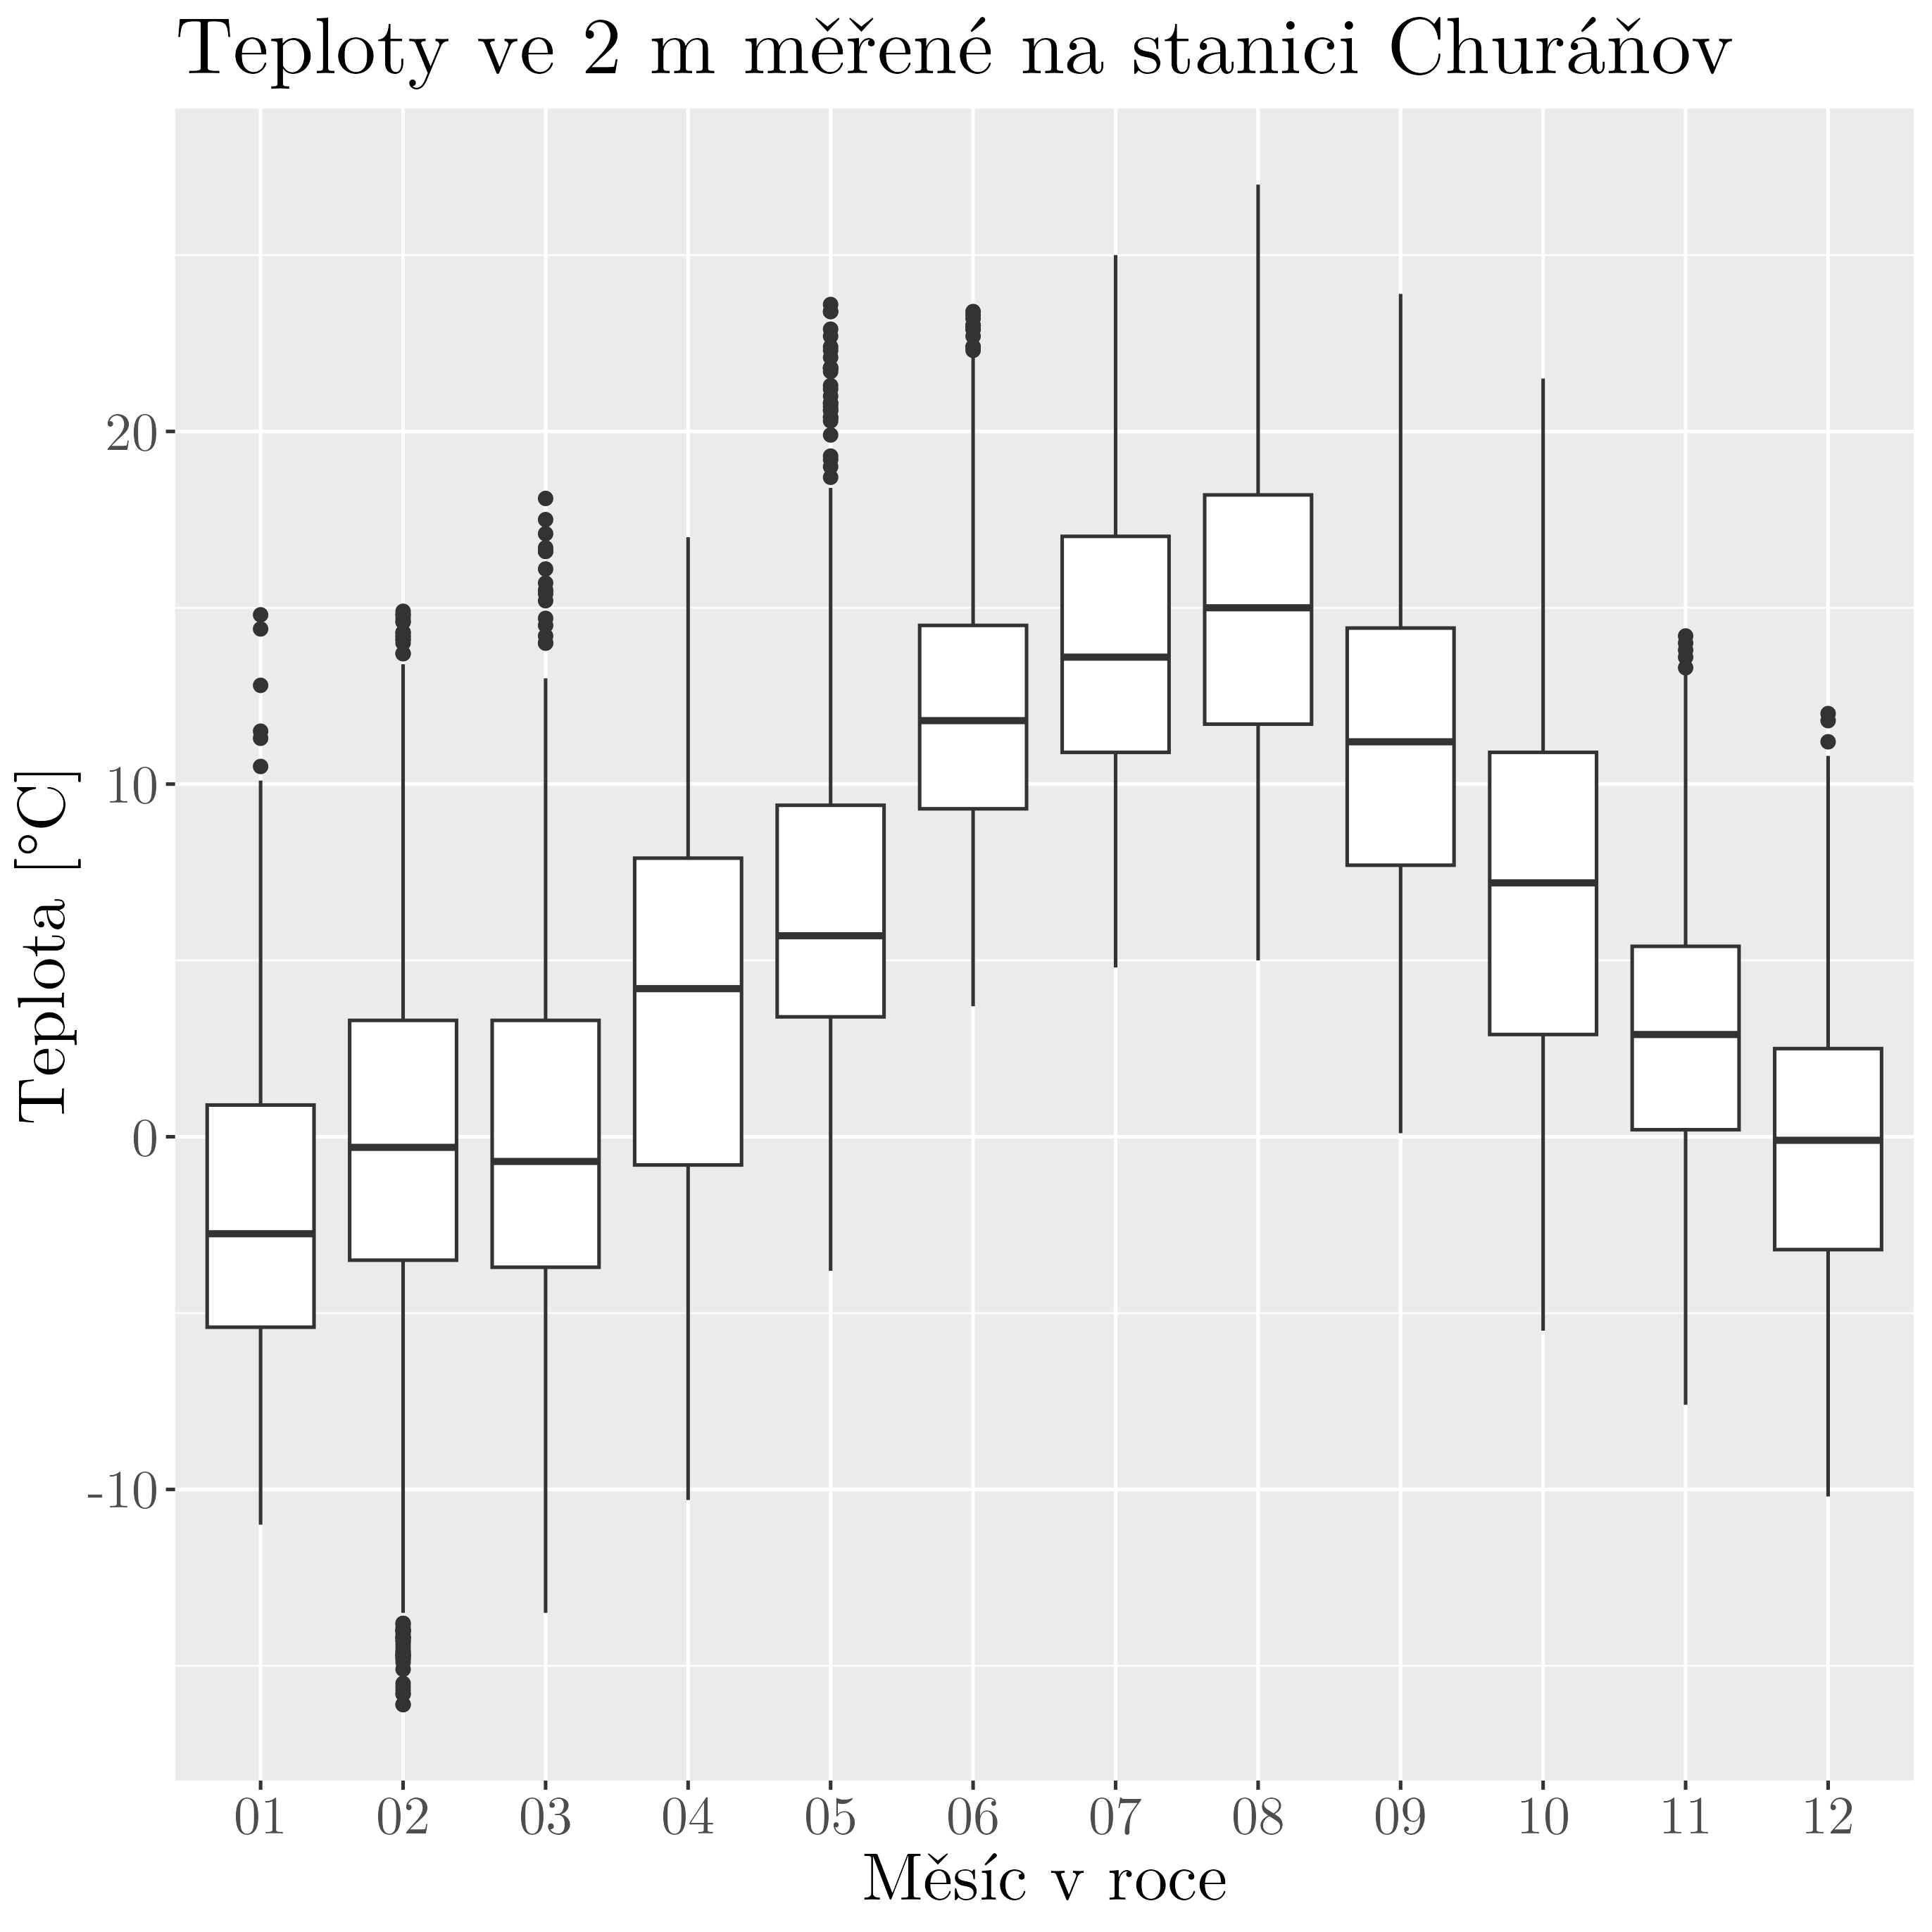
\includegraphics[width=\textwidth]{img/synop_temperature.png}
		\caption{}
		\label{fig:synop_temperature}
	\end{subfigure}
	\hfill
	\begin{subfigure}{0.45\textwidth}
  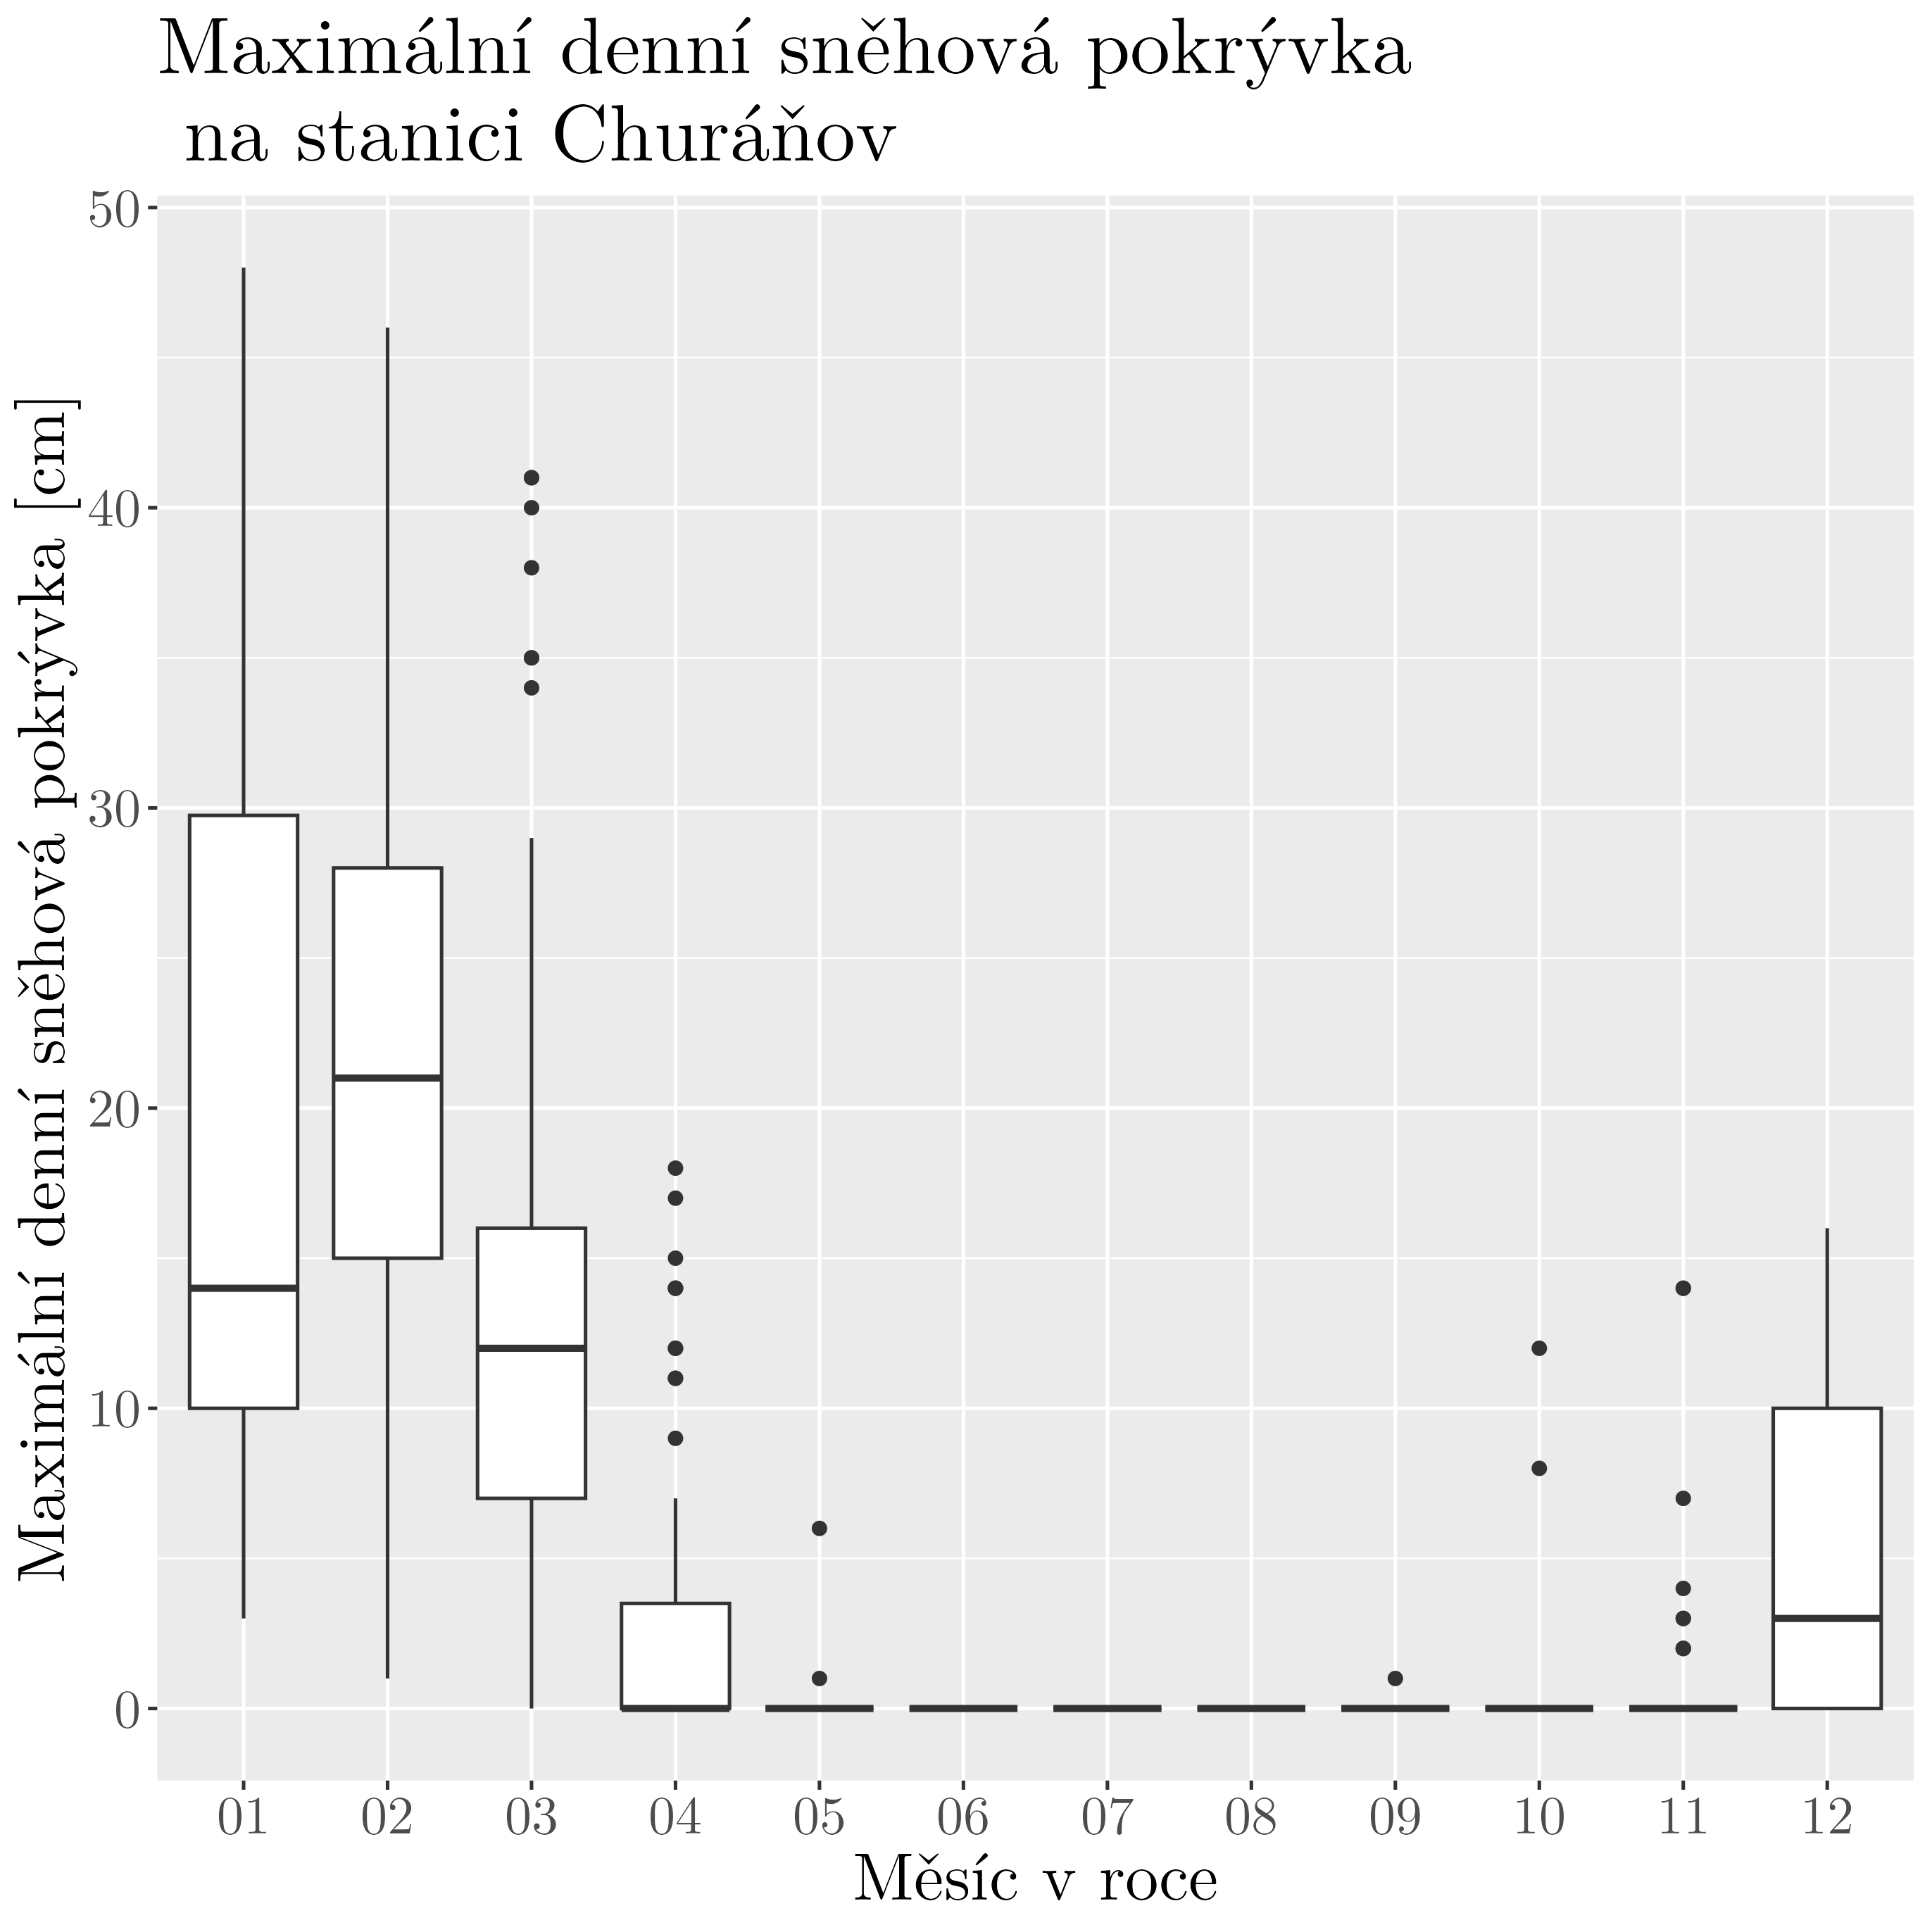
\includegraphics[width=\textwidth]{img/synop_snowcm.png}
		\caption{}
		\label{fig:synop_snowcm}
	\end{subfigure}
	\hfill
	\begin{subfigure}{0.45\textwidth}
  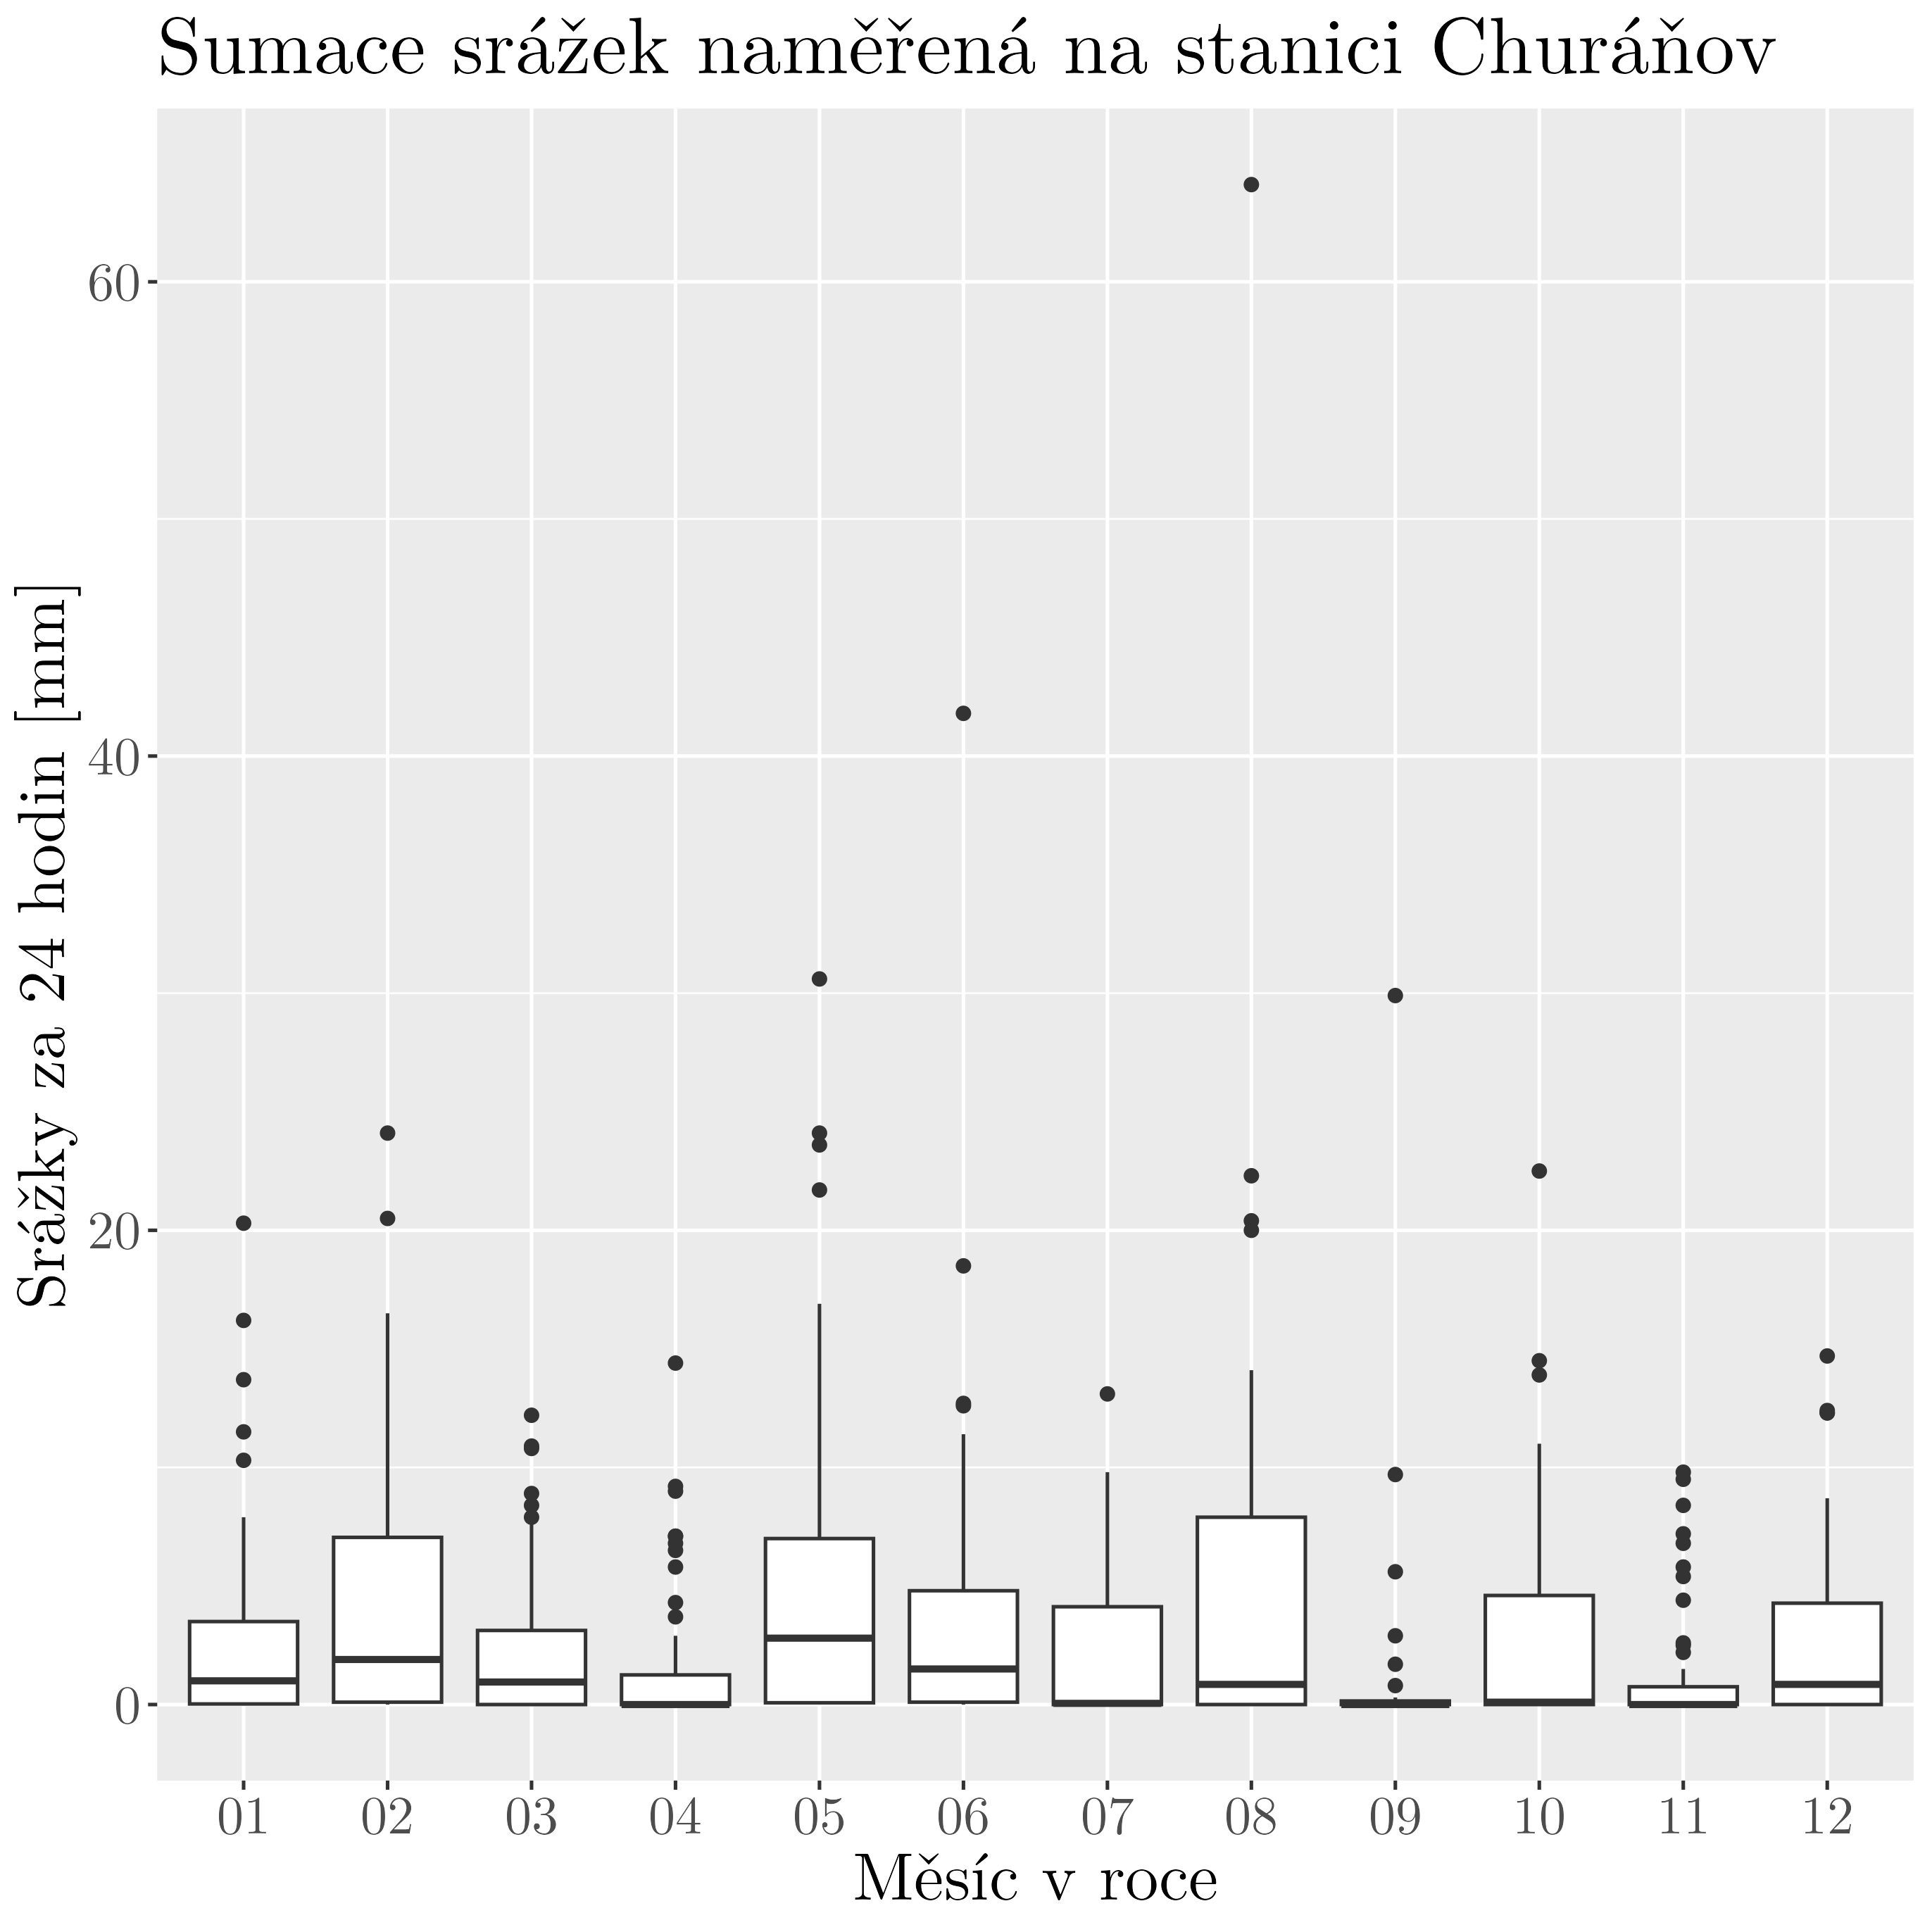
\includegraphics[width=\textwidth]{img/synop_prec.png}
		\caption{}
		\label{fig:synop_prec}
	\end{subfigure}
	\hfill
	\begin{subfigure}{0.45\textwidth}
  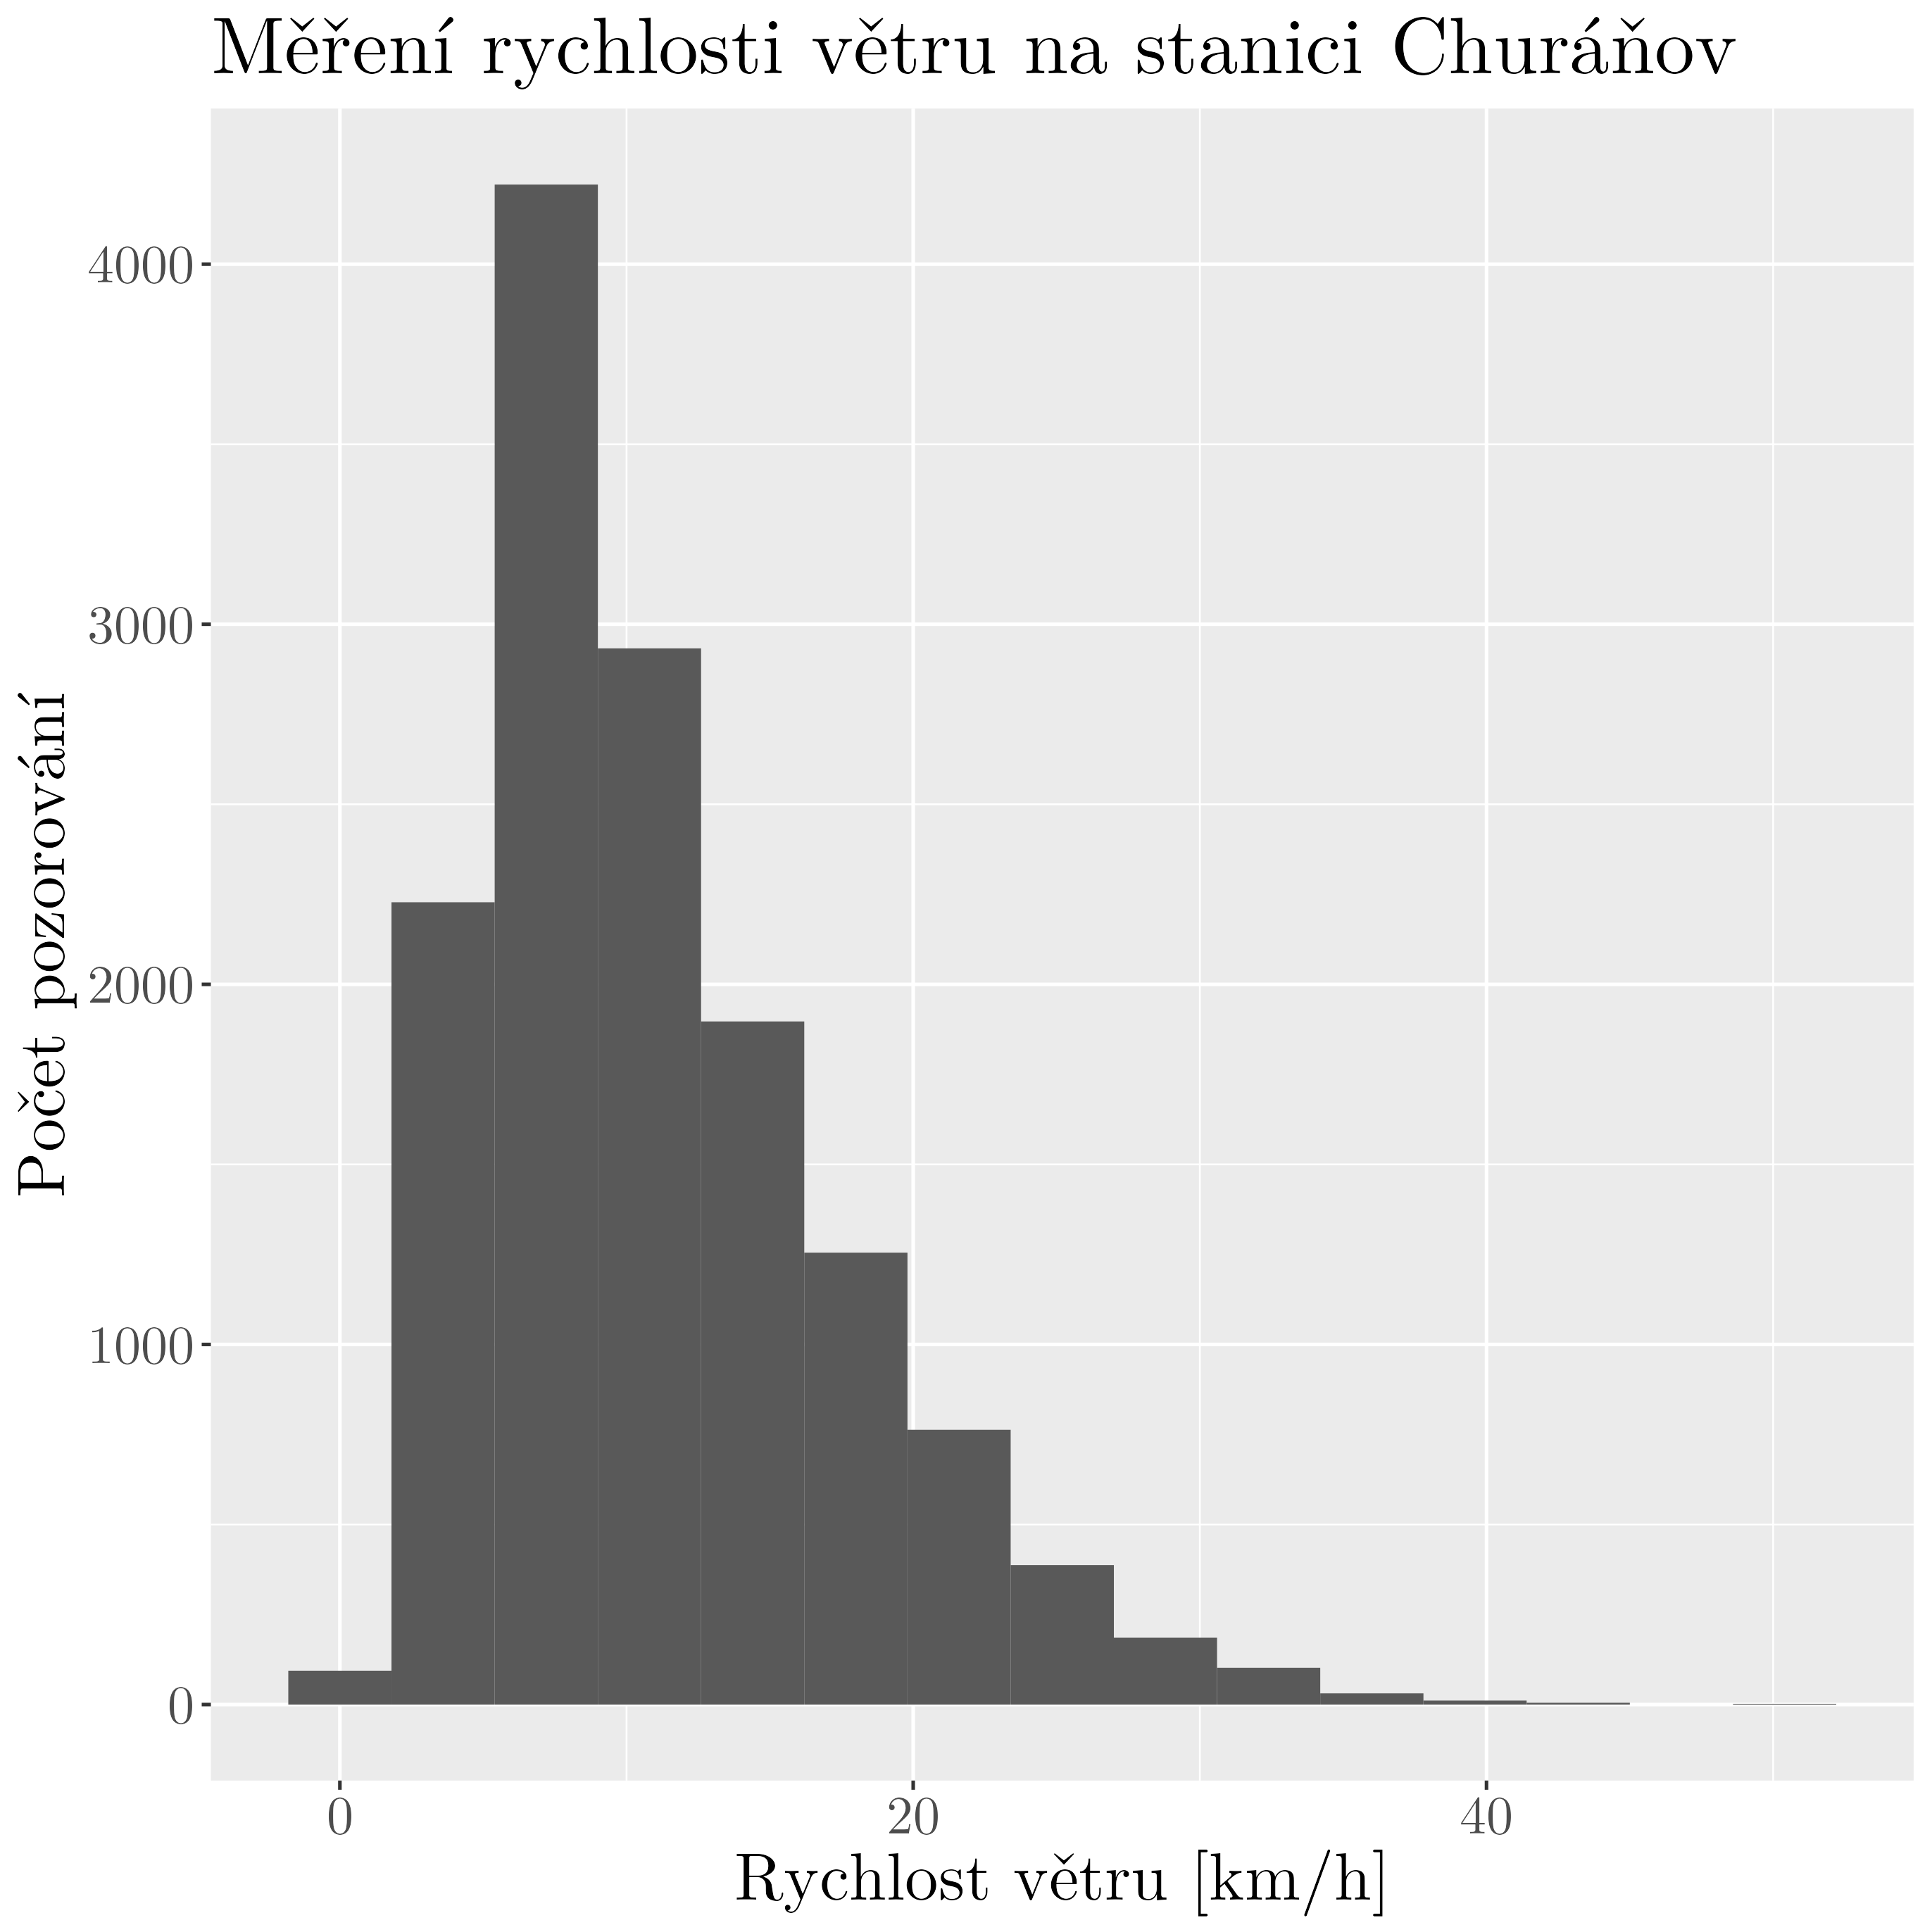
\includegraphics[width=\textwidth]{img/synop_ffkmh.png}
		\caption{}
		\label{fig:synop_ffkmh}
	\end{subfigure}
	\caption{Data ze synoptické stanice Churáňov za období 12.10.2019 až 20.5.2021} 
	\label{fig:chmuukazka}
\end{figure}

Meteorologická stanice Churáňov měřící podle principů popsaných v kapitole \ref{chap:meteostations}. Zaznamenává tedy oblačnost každou hodinu. Data jsou zaznamenávána pouze přes den, v noci máme chybějící hodnoty. Maximální teploty jsou typicky dosažené během dne, kdy většinou oblačnost známe. Například v zimě pod sněhem může maximální denní teplota být dosažena i v noci. Minimální denní teploty na druhou stranu typicky nastávají během ranních hodin, po východu Slunce, ale ojediněle i před ním (viz kapitola \ref{chap:showingoffdata} a obrázek \ref{fig:hours}). Pro minimální teploty nám tedy často chybí odpovídající oblačnost. Vyřazení těchto hodnot by vložilo velké zkreslení do dat, tudíž byla zvolena cesta, kdy využijeme data z projektu ERA5.

Pro každou hodnotu, která chybí ze staničního měření použijeme nejbližší hodnotu z ERA5 a to konkrétně z $\SI{49}{\degree}$ severní šířky a $\SI{13.5}{\degree}$ východní délky. Tato data byla vzdálená od stanice Churáňov $\SI{14.8}{km}$. V kapitole \ref{chap:disc_era5} budeme diskutovat vliv nahrazení dat pomocí ERA5.

\section{Data z BÚ AV}\label{chap:data_buav}
Data poskytnutá Botanickým ústavem Akademie věd České republiky byla naměřená dvěma typy čidel popsanými v kapitole \ref{chap:loggers}. Nadále se budeme zabývat pouze těmi plochami, které jsou opatřeny jak pozemními čidly, tak čidly ve standartní výšce $\SI{2}{m}$. Na obrázku \ref{fig:rozlozenicidel} můžeme vidět jejich prostorové rozložení, celkově jde o 157 čidel. 

Umístění čidel bylo vybíráno tak aby pokryly gradienty nadmořské výšky (5 tříd), potenciální solární radiace, určující množství záření, které dopadá na zem (3 třídy) a topografického vlhkostního indexu, který kombinuje svažitost a akumulaci vody v terénu (3 třídy). Plochy byly dále doplněny tak, aby bylo rovnoměrně pokryto území národních parků, a aby se nevyskytovaly poblíž turistických stezek.

\begin{figure}
	\centering
	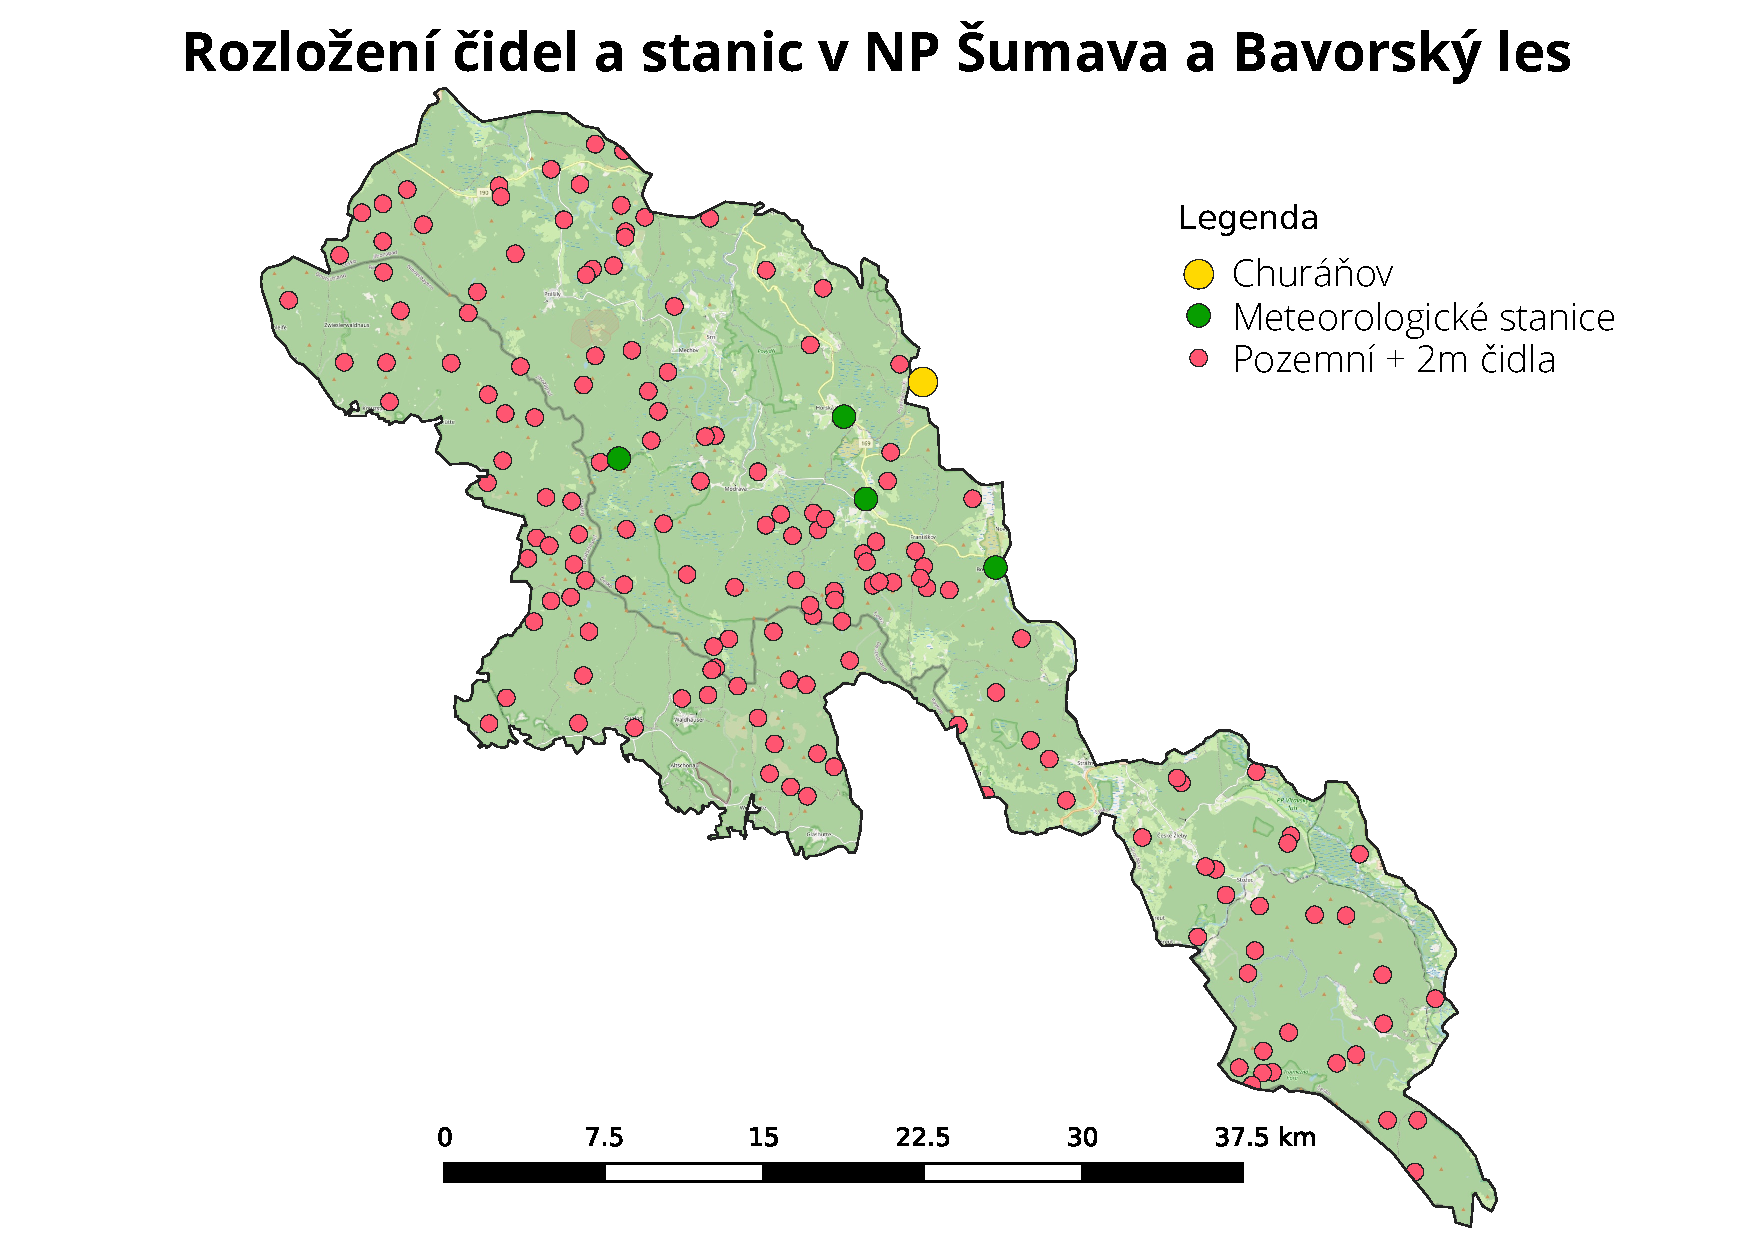
\includegraphics[width=0.95\textwidth]{img/rozlozenicidel.pdf}
	\caption{Rozložení čidel a meteorologický stanic napříč Národním parkem Šumava ($N=112$) a Národním parkem Bavorský les ($N=45$)}
	\label{fig:rozlozenicidel}
\end{figure}

Data vykazují malou chybovost, duplicitní a chybějící záznamy byly vyřazeny. Dále byla data vizuálně překontrolována. Části, kdy byla čidla např. povytažená ze země (pozná se podle hodnot půdní vlhkosti), byly nahrazeny hodnotami NA. Podobně pokud čidlo T1 spadlo ze stromu, tak jsou hodnoty nahrazeny NA. Toto čištění dat provedli RNDr. Josef Brůna, Ph.D., doc. Ing. Jan Wild, Ph.D. a další, s jejichž svolením jsou data využitá v této práci. Ve velmi ojedinělých případech chyběly odpovídající hodnoty teplot ve $\SI{2}{m}$, v době kdy při zemi nastalo denní maximum nebo minimum. Pokud existovaly hodnoty až 30 minut starší tak jsme použily tyto, v opačném případě jsme čidlo pro daný den vyřadili, šlo o jednotky případů.

Dostupnost dat z čidel je vidět na obrázku \ref{fig:dostupnostdat}, vidíme zde dvě skupiny čidel, jedny, nacházející se v Národním parku Bavorský les mají dostupná data pro cca 400 dnů. Čidla z Národního parku Šumava mají dostupná data pro téměř 600 dnů. Na obrázku \ref{fig:dostupnostdnu} vidíme, na kolika čidlech jsou zastoupeny jednotlivé dny.

\begin{figure}
	\centering
	\begin{subfigure}{0.45\textwidth}
  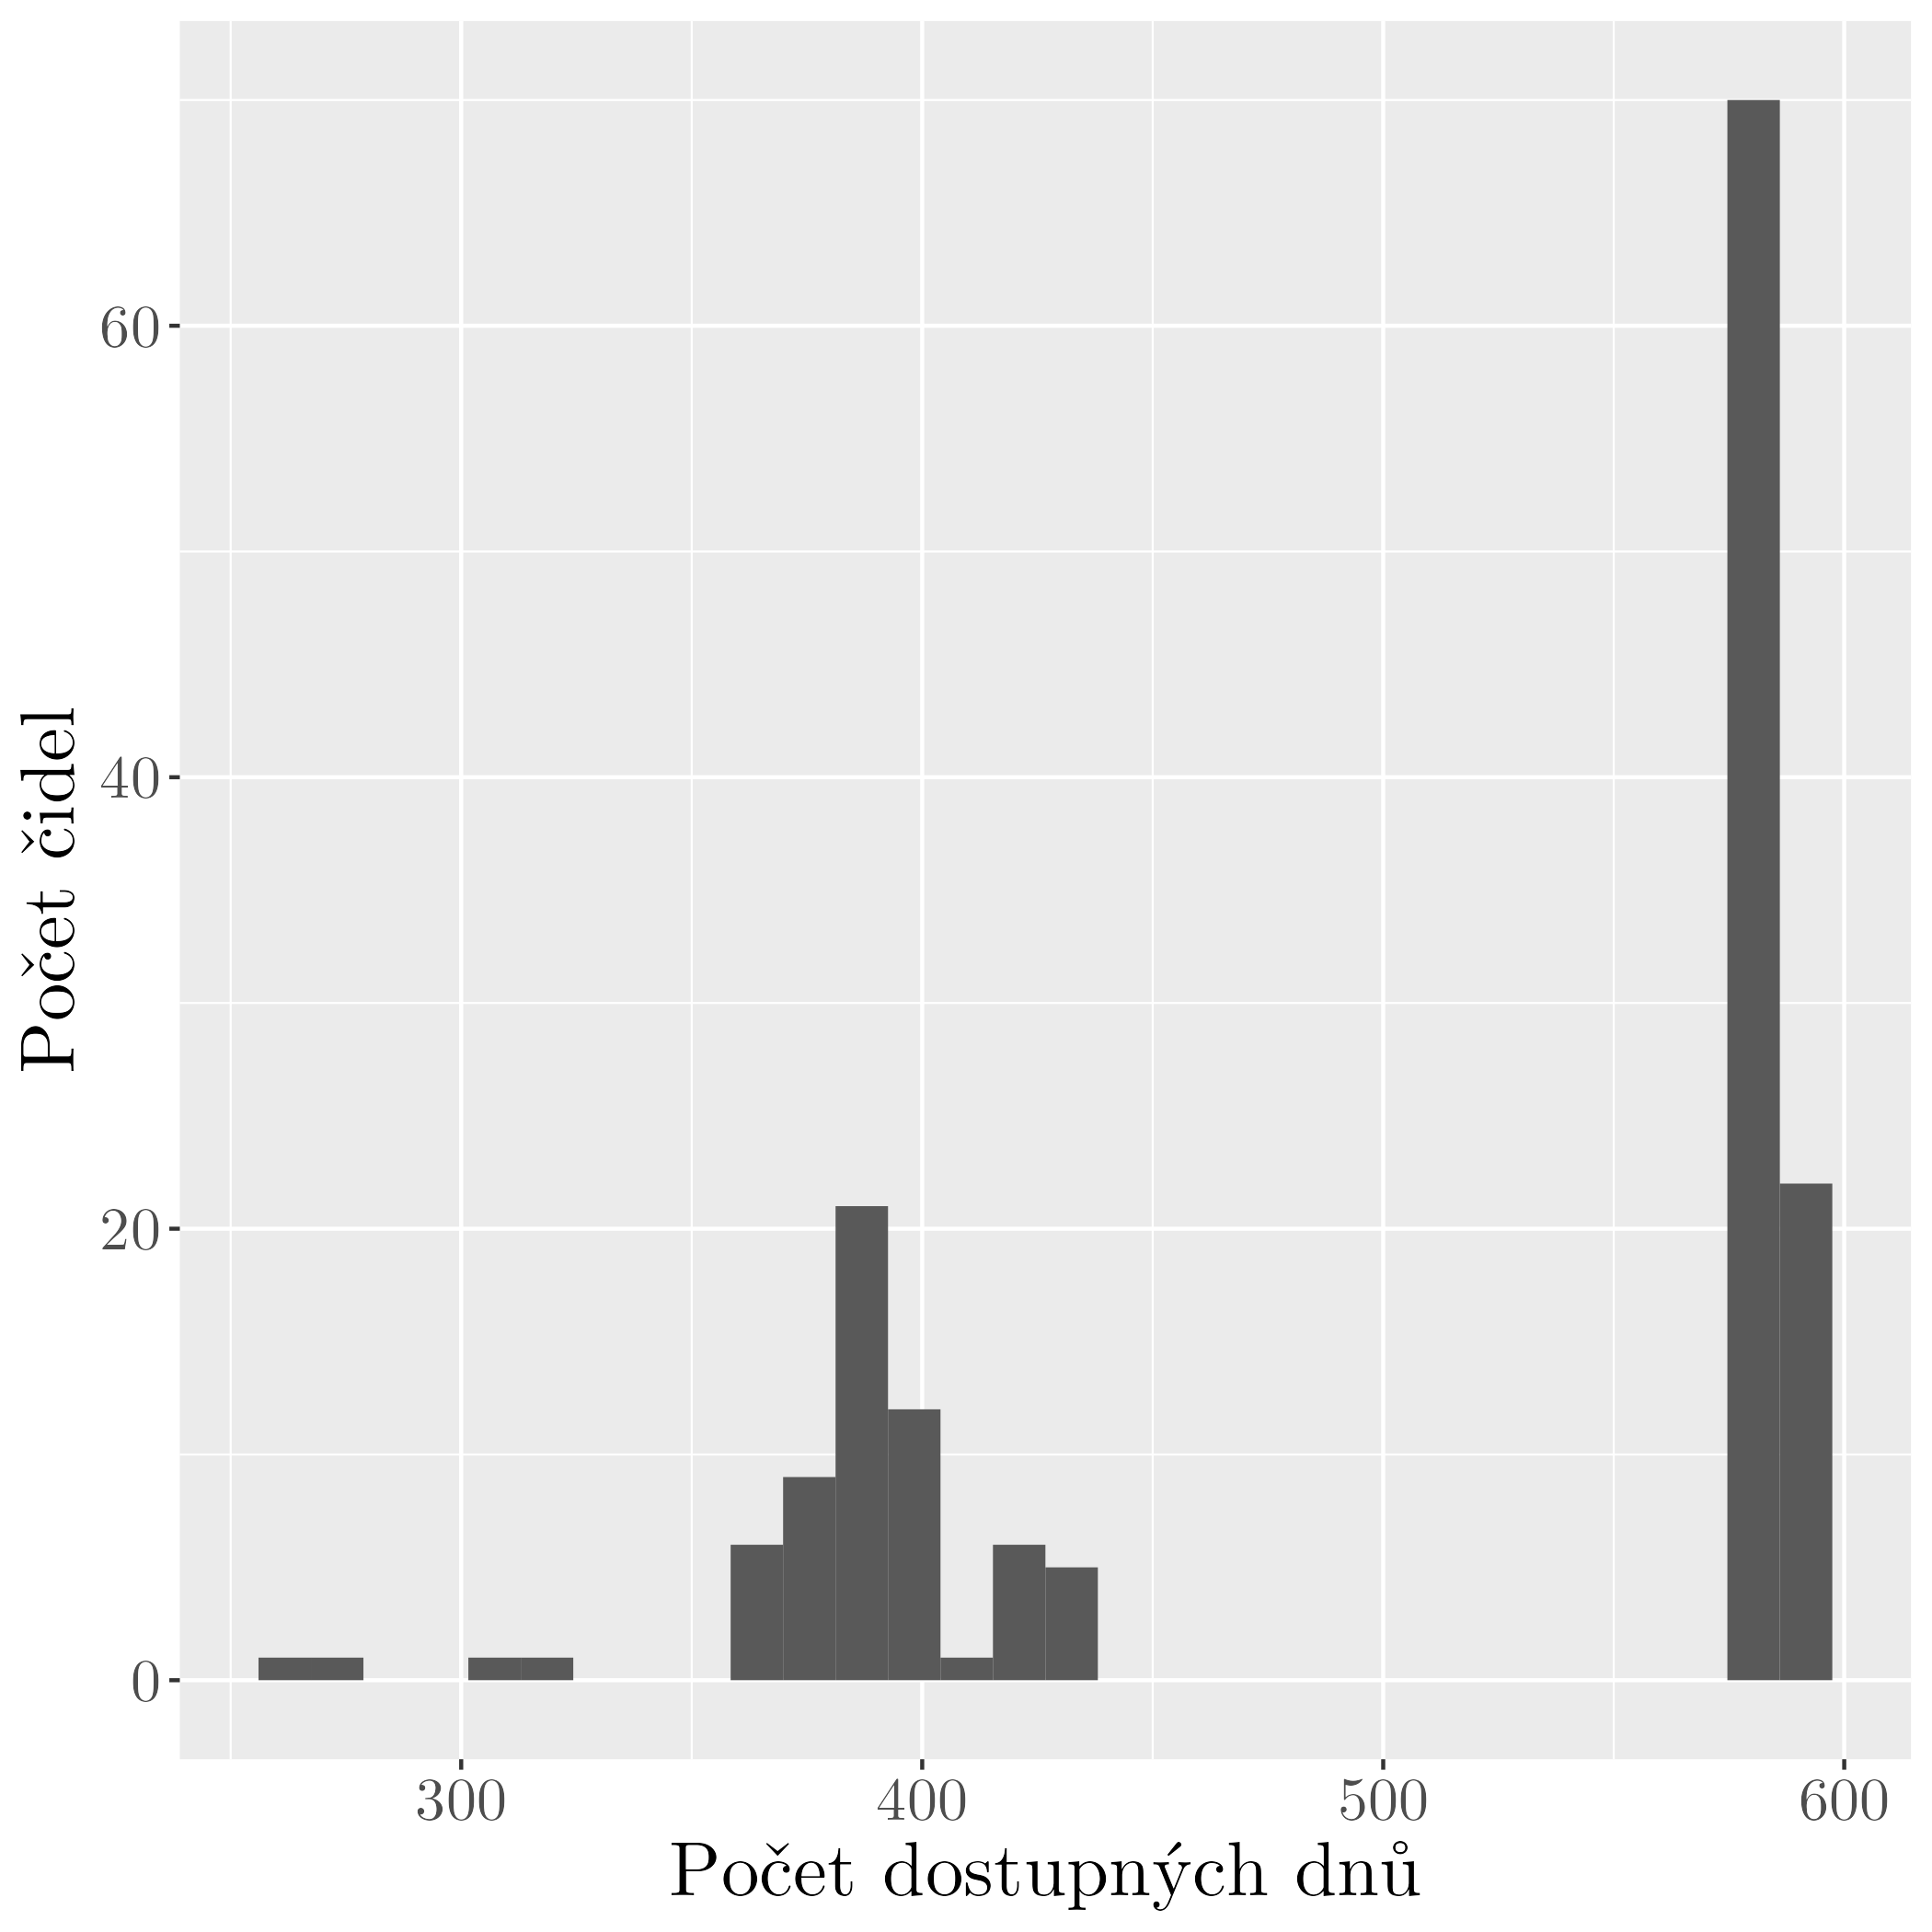
\includegraphics[width=\textwidth]{img/hist_numofdayavailability.png}
	\caption{Histogram ukazující množství dostupných dnů pro jednotlivá čidla}
	\label{fig:dostupnostdat}
	\end{subfigure}
	\hfill
	\begin{subfigure}{0.45\textwidth}
  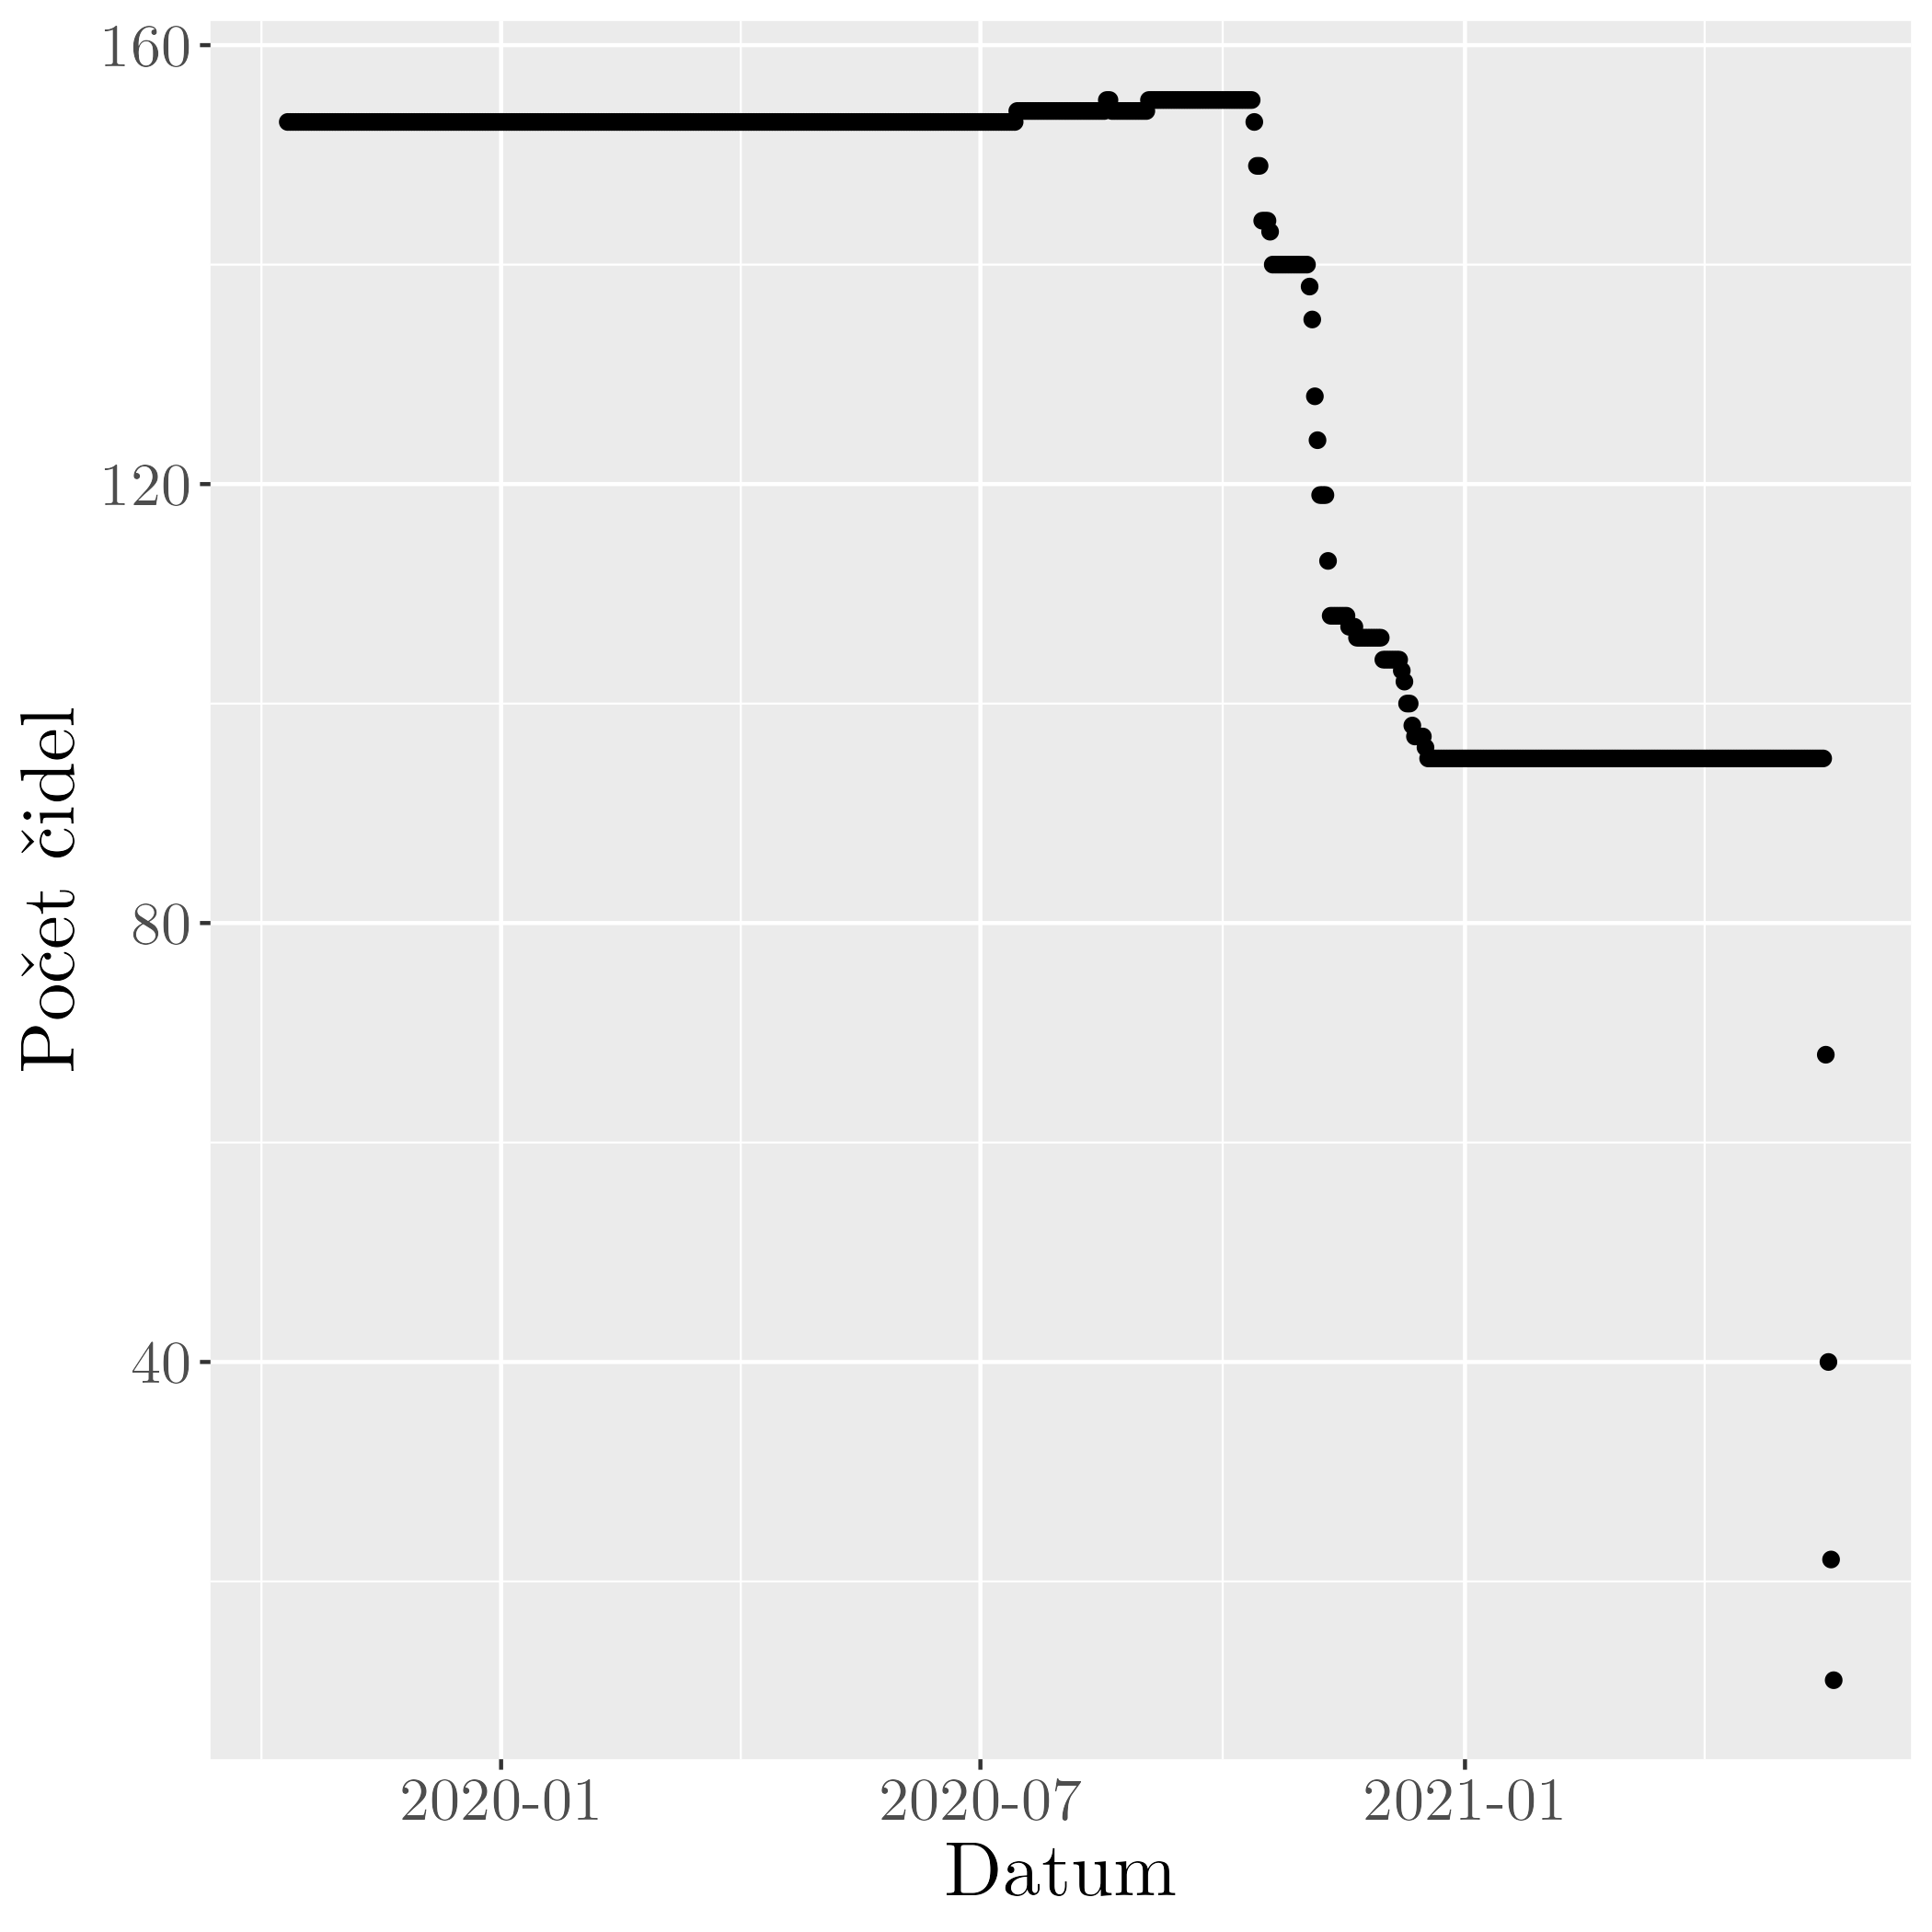
\includegraphics[width=\textwidth]{img/date_availability.png}
	\caption{Graf zastoupení čidel pro jednotlivé dny}
	\label{fig:dostupnostdnu}
	\end{subfigure}
	\caption{Dostupnost dat z čidel}
\end{figure}

Pro samotné zpracování jsme vyřadili poslední 4 dny v květnu, protože mají menší počet čidel z kterých máme v té době měření. Tímto se dostáváme na interval dat od 12.10.2019 do 17.5.2021.

\section{Insolace}
Na obrázku \ref{fig:insolacelogger} můžeme vidět hodnoty insolace spočtené podle odstavce \ref{chap:insolation} pro čidlo, které je nejblíž stanici Churáňov. Sinusoida nám téměř určuje hodnotu maximální denní insolace. Ve většině případů nejde o maximum, protože maximální denní teploty nastávají většinou později než maximum insolace. Také pracujeme na časovém měřítku 15 minut, a tedy je malá pravděpodobnost, že se maximální denní teplota trefí do maxima insolace. Nulové hodnoty odpovídají dennímu maximumu v noci (typicky kvůli přítomnosti sněhu), a tudíž má insolace nulovou hodnotu.

\begin{figure}
	\centering
	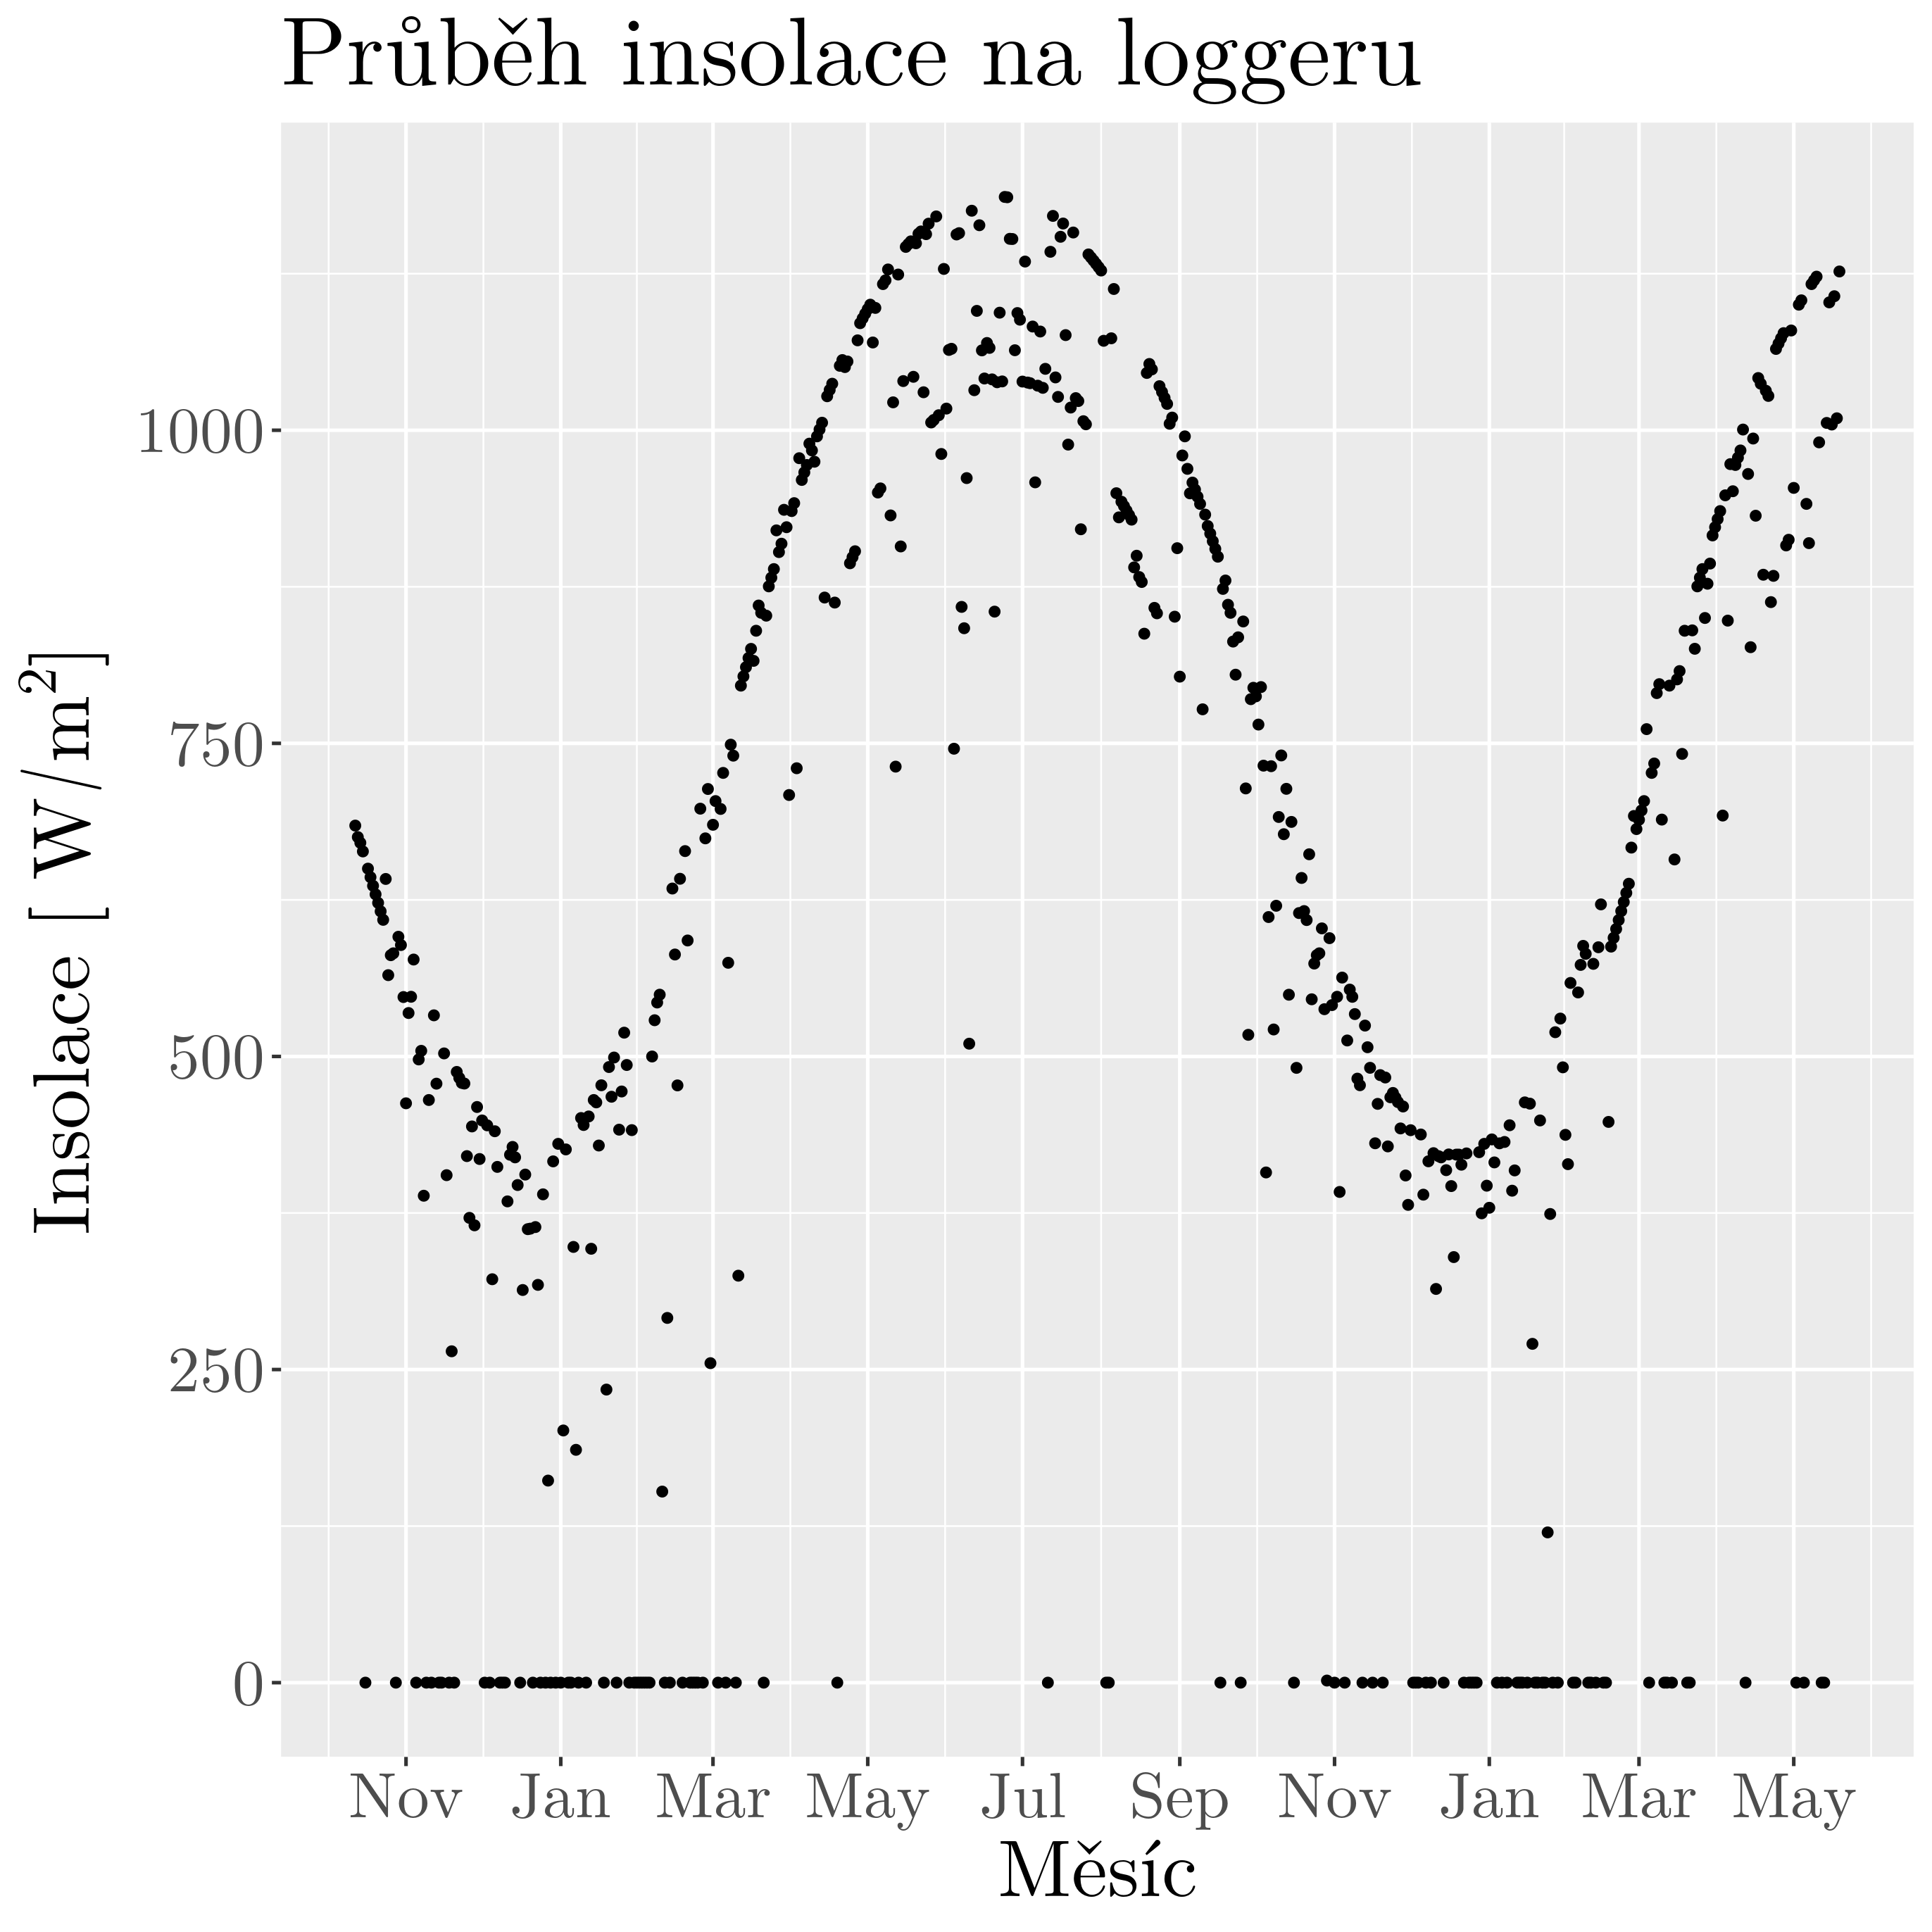
\includegraphics[width=0.65\textwidth]{img/ch2/insolation_max15cmNPS_4311_D_TMS.png}
	\caption{Hodnoty insolace na čidlu nejblíže stanici Churáňov v době dosažení maximální denní teploty ve výšce $\SI{15}{cm}$.}
	\label{fig:insolacelogger}
\end{figure}

\section{Explorace použitých dat}\label{chap:showingoffdata}
Dále se podívejme na ukázku dat naměřených na čidlech. Na obrázcích \ref{fig:hours} můžeme vidět kdy nastávaly maximální a minimální teploty ve výškách $\SI{0}{cm}$ a $\SI{15}{cm}$ nad zemí, denní hodina je uvedená v UTC, nikoliv SEČ nebo SELČ. U maximálních teplot si můžeme všimnout kromě maxima v okolí 10 UTC také menšího maxima a odlehlých hodnot způsobených přítomností sněhu v zimě. Podobně měl sníh vliv i na dobu minimálních teplot v zimě.

\begin{figure}
	\centering
	\begin{subfigure}{0.45\textwidth}
  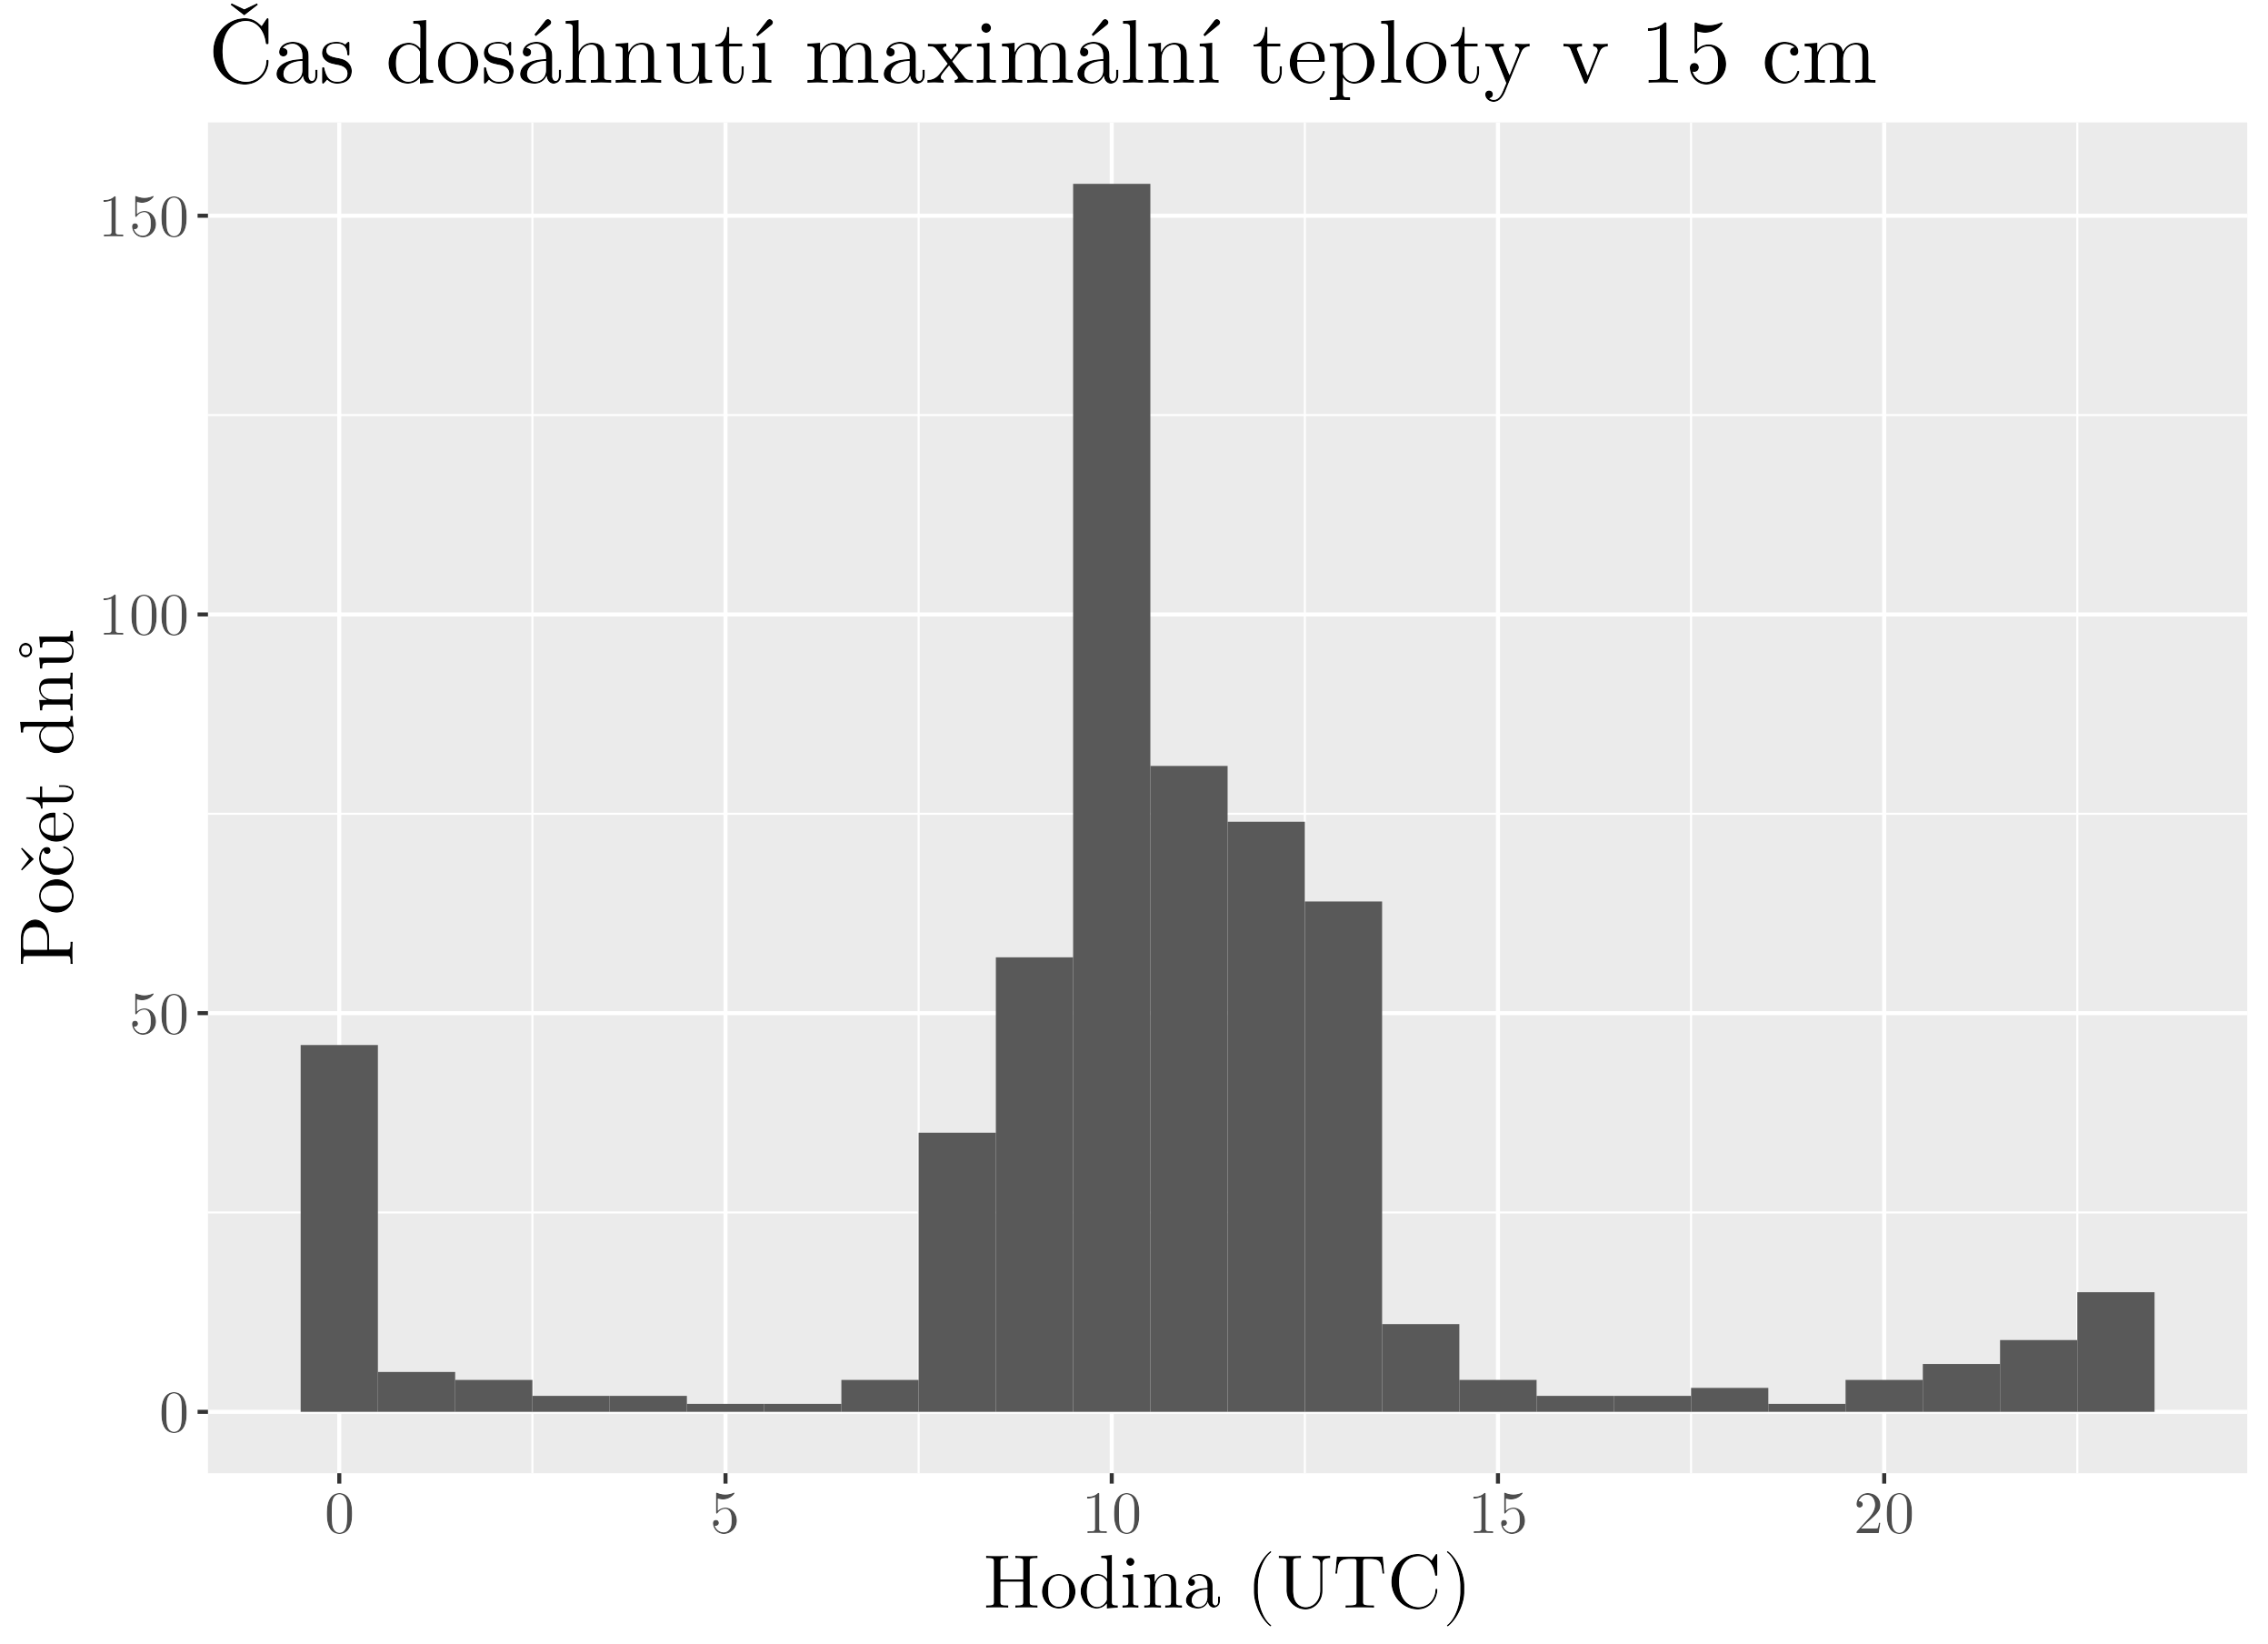
\includegraphics[width=\textwidth]{img/hist_hourmax15cm.png}
		\caption{}
		\label{fig:hourmax15cm}
	\end{subfigure}
	\hfill
	\begin{subfigure}{0.45\textwidth}
  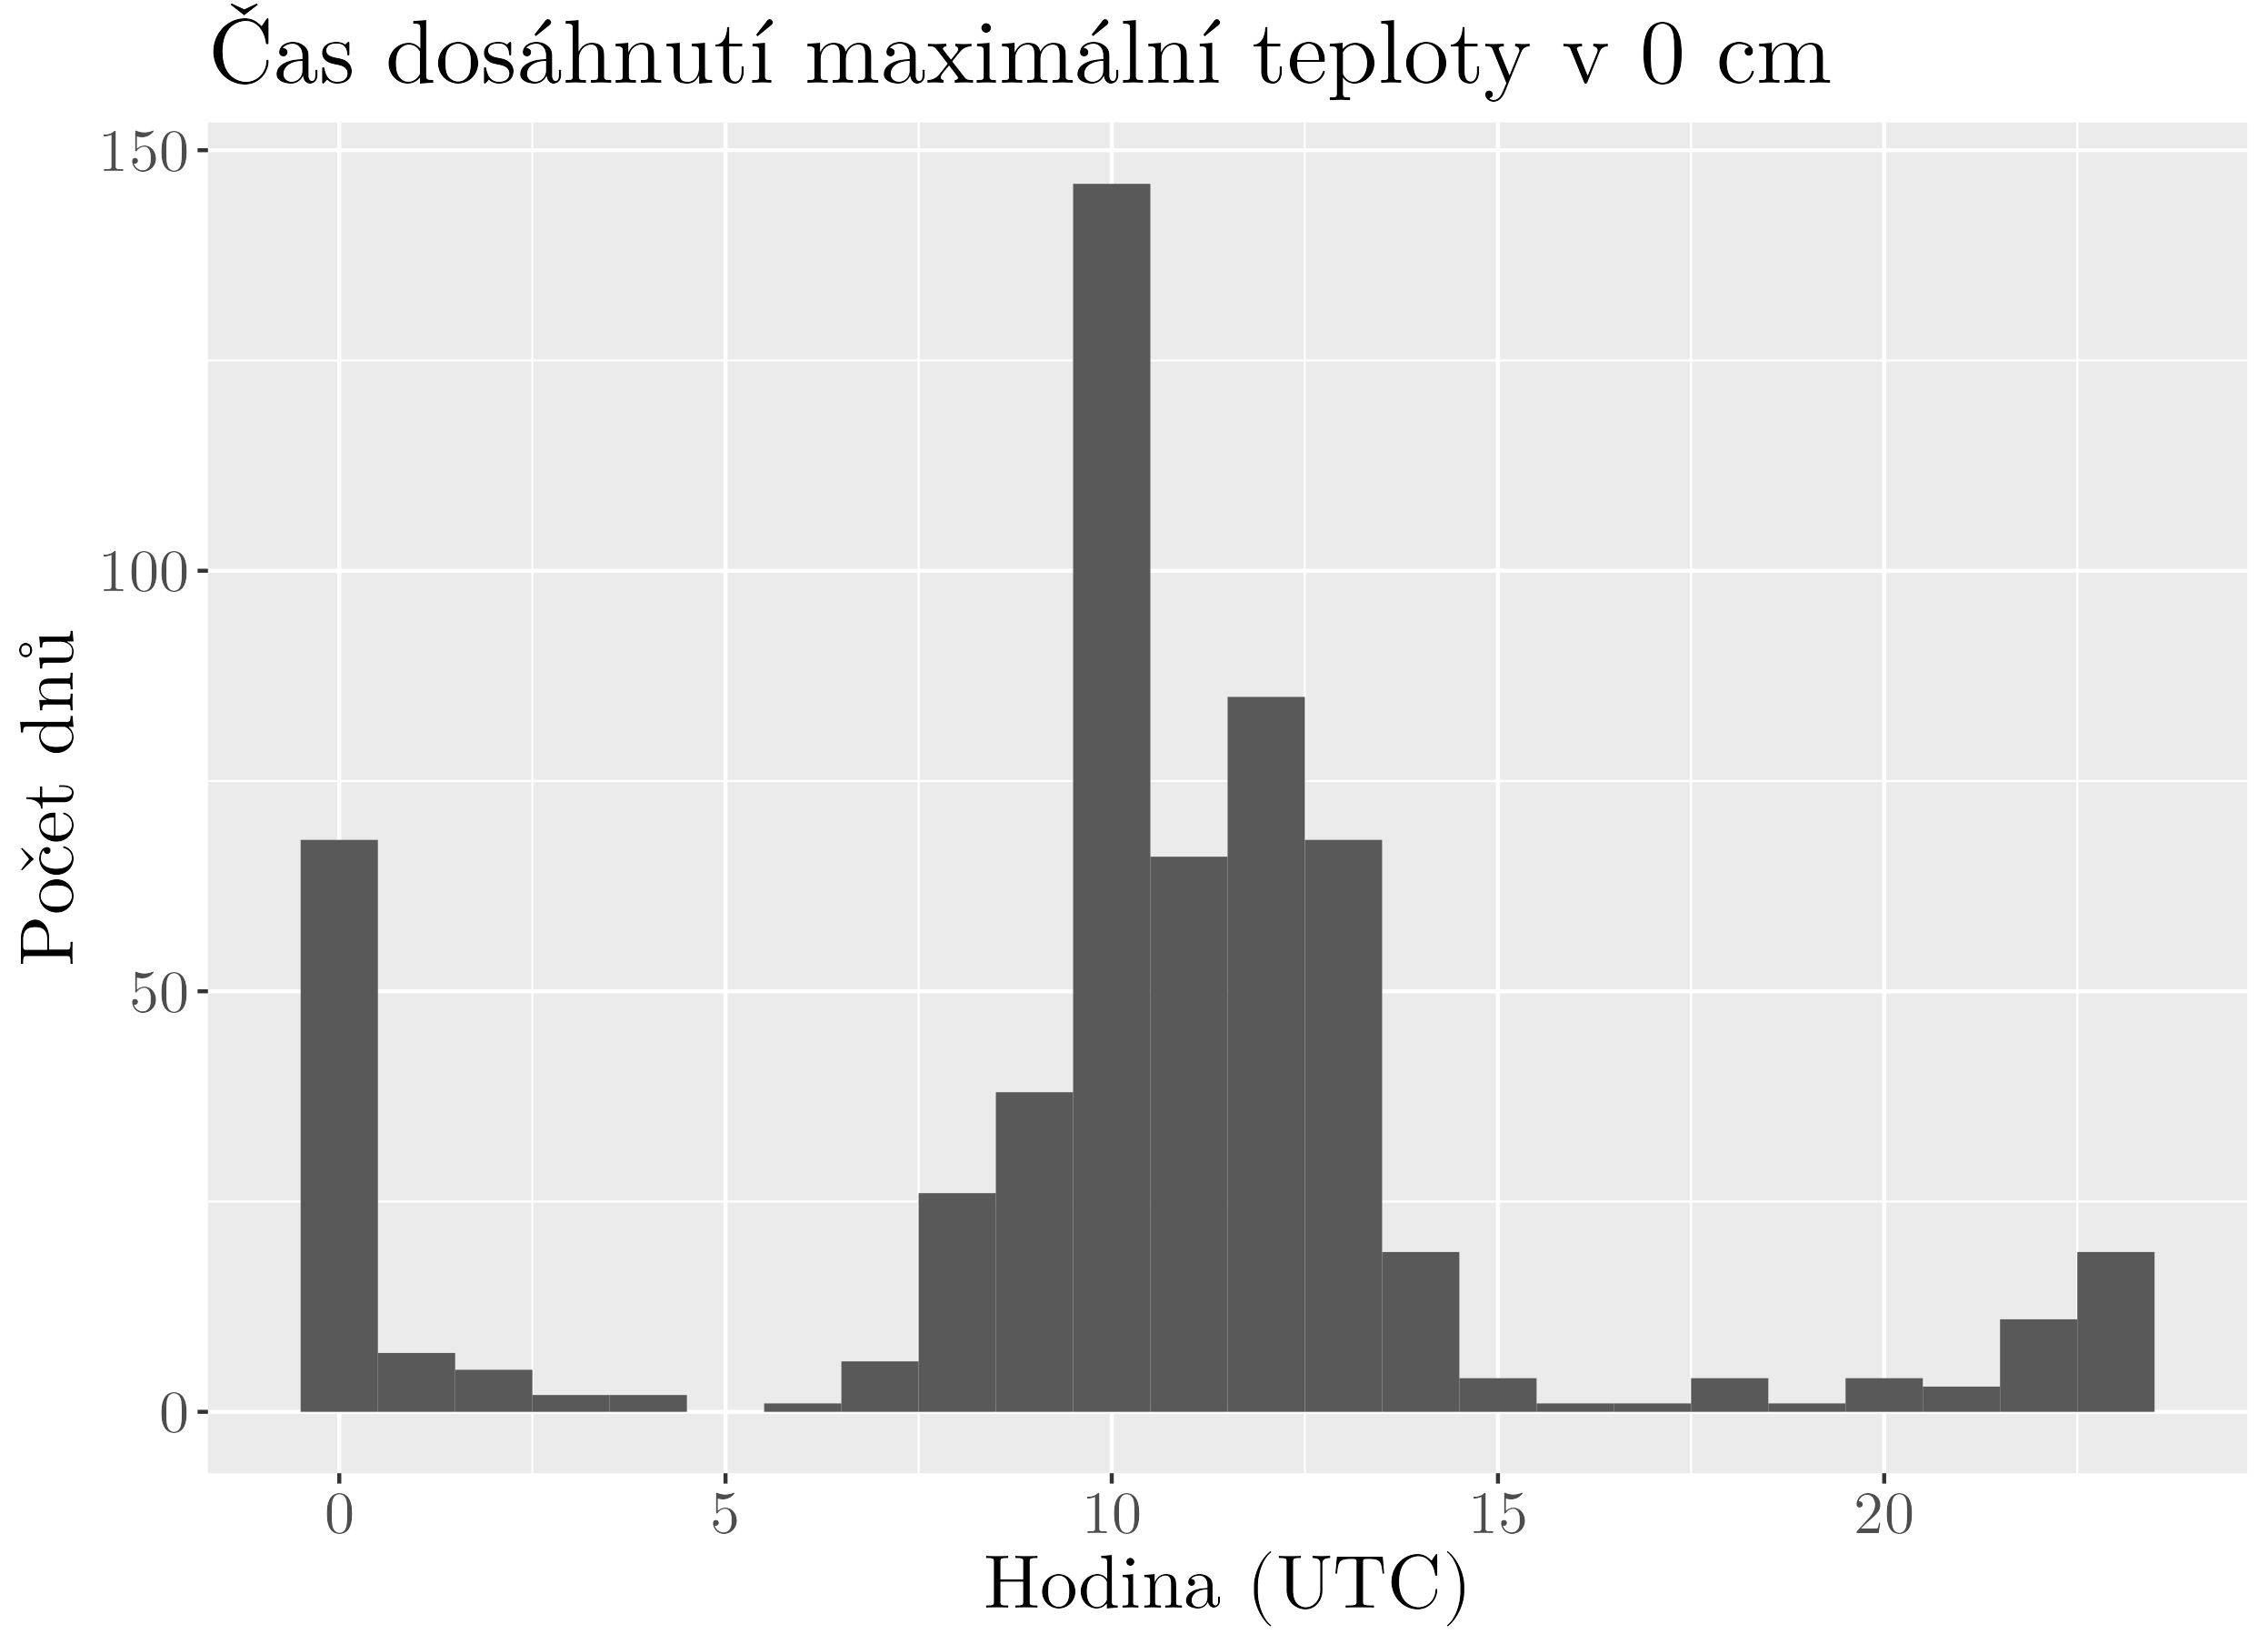
\includegraphics[width=\textwidth]{img/hist_hourmax0cm.png}
		\caption{}
		\label{fig:hourmax0cm}
	\end{subfigure}
	\hfill
	\begin{subfigure}{0.45\textwidth}
  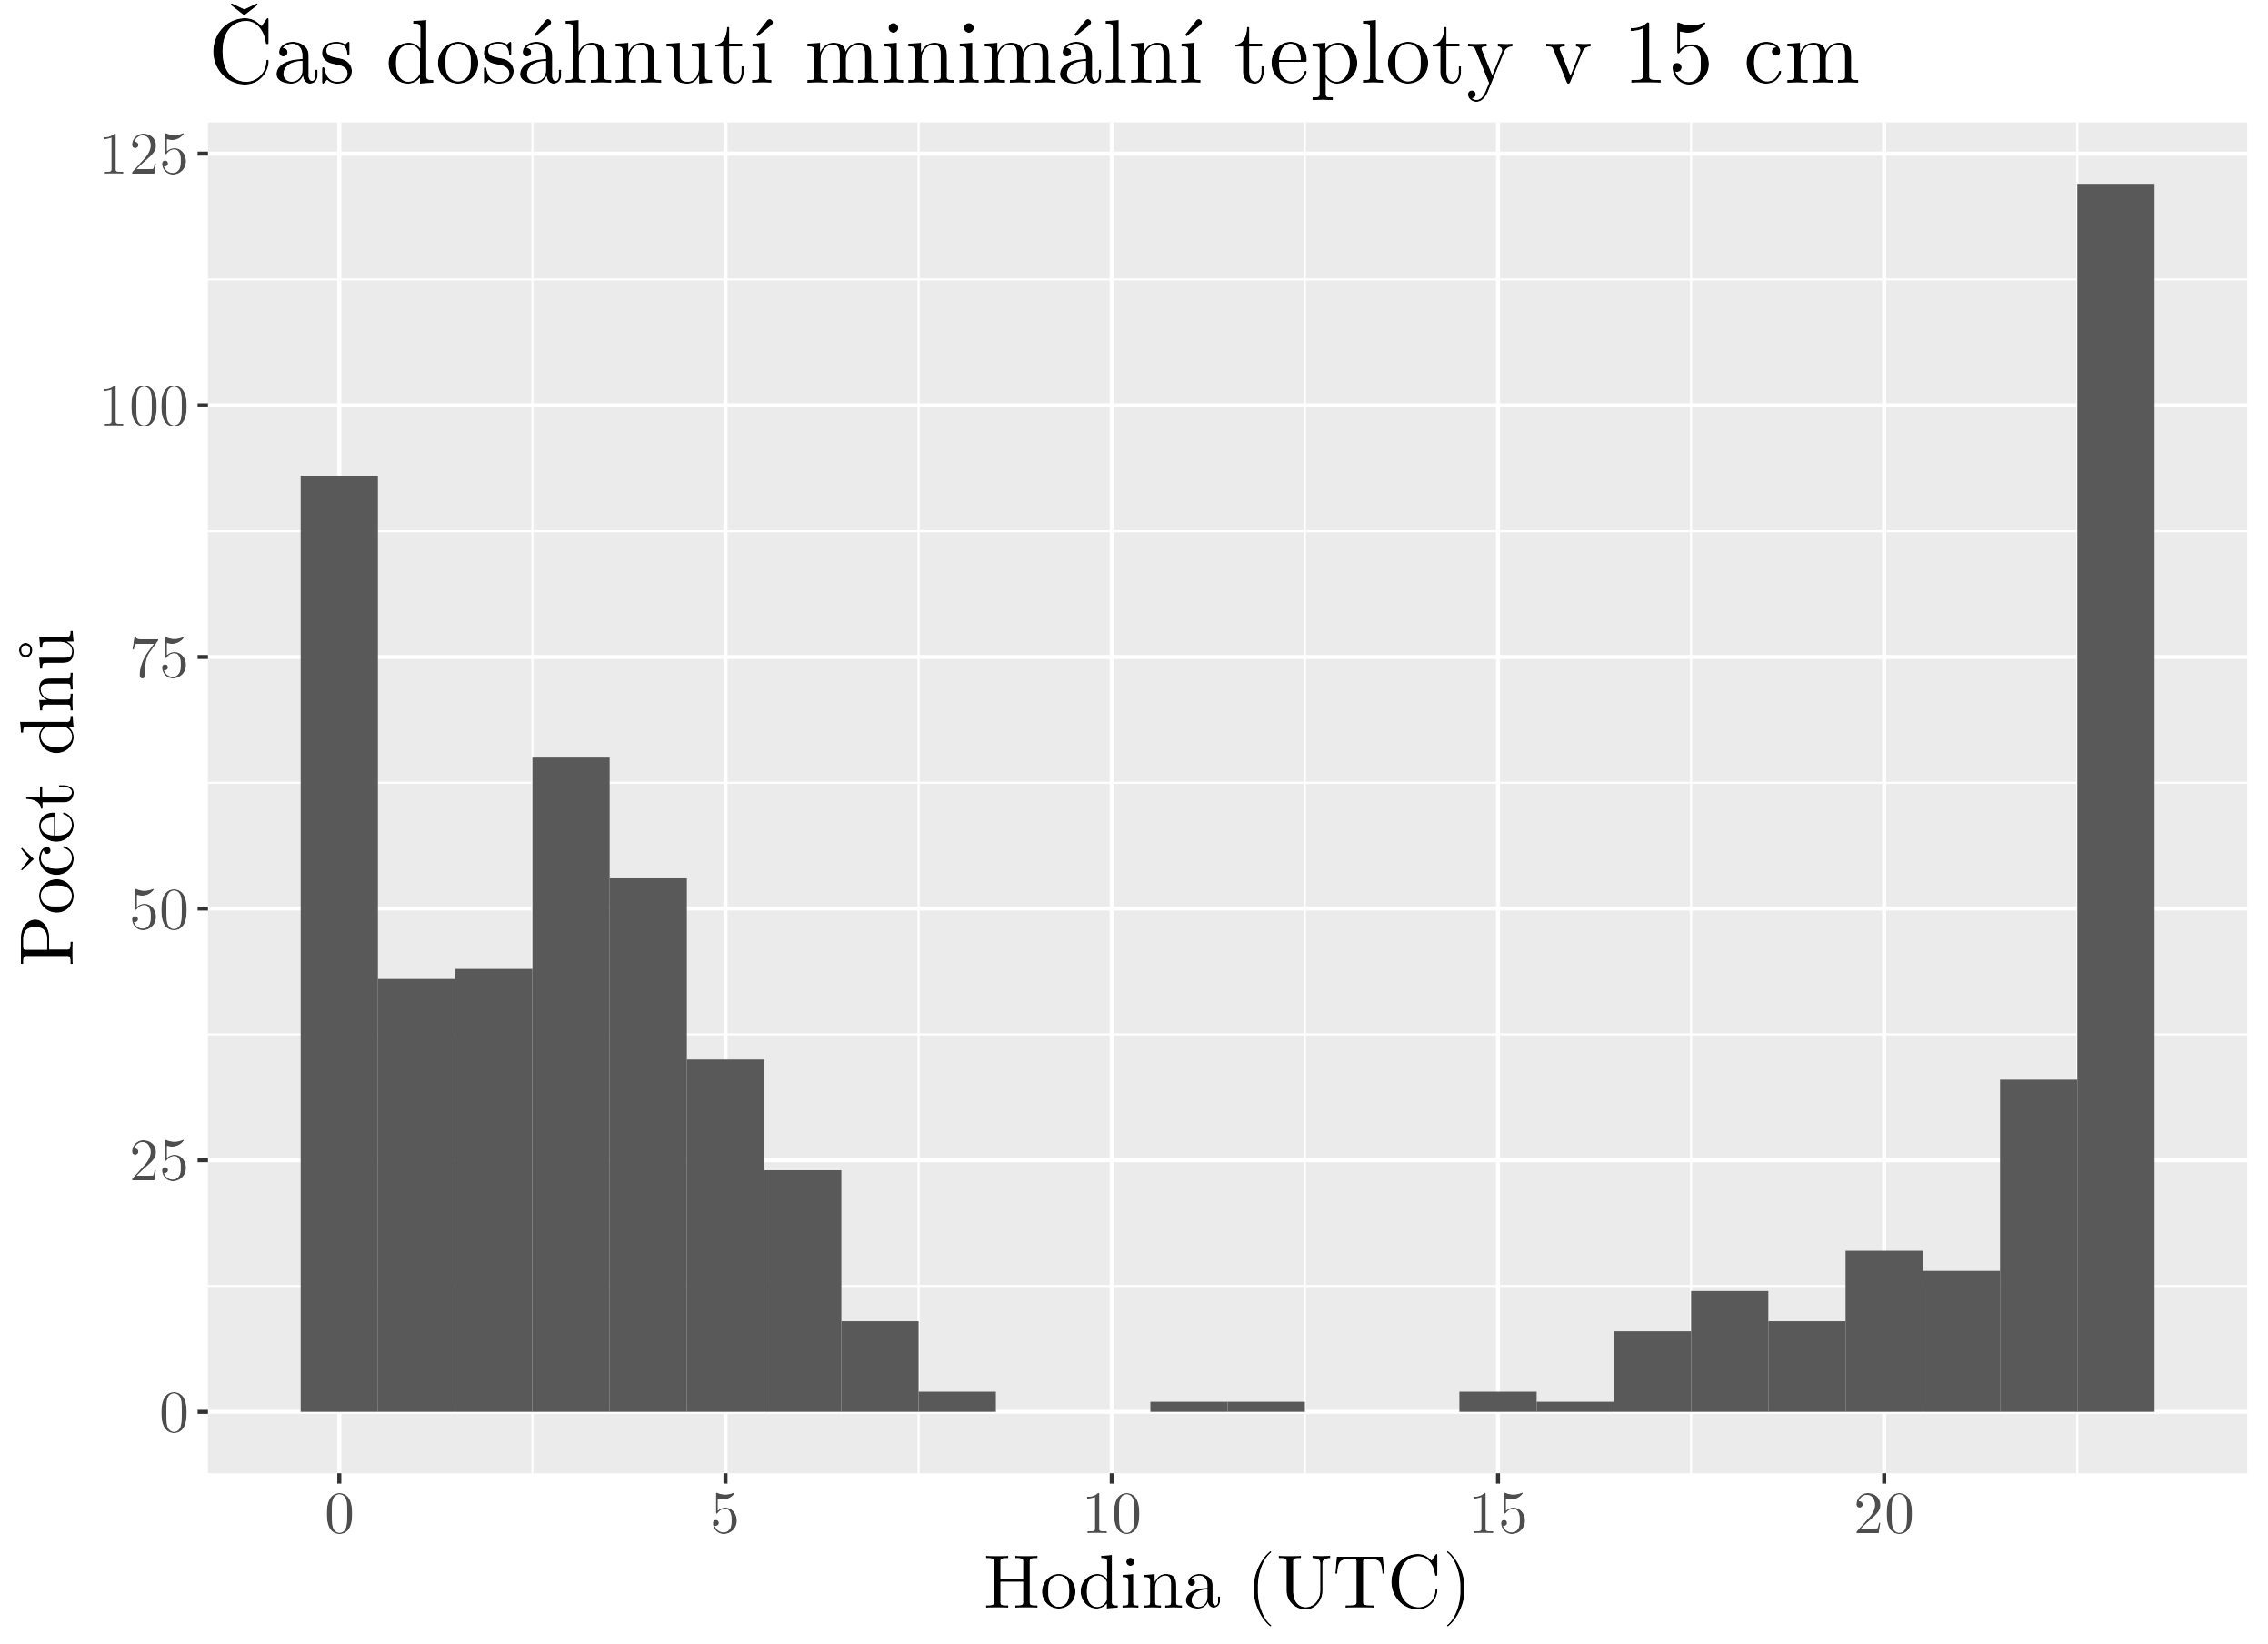
\includegraphics[width=\textwidth]{img/hist_hourmin15cm.png}
		\caption{}
		\label{fig:hourmin15cm}
	\end{subfigure}
	\hfill
	\begin{subfigure}{0.45\textwidth}
  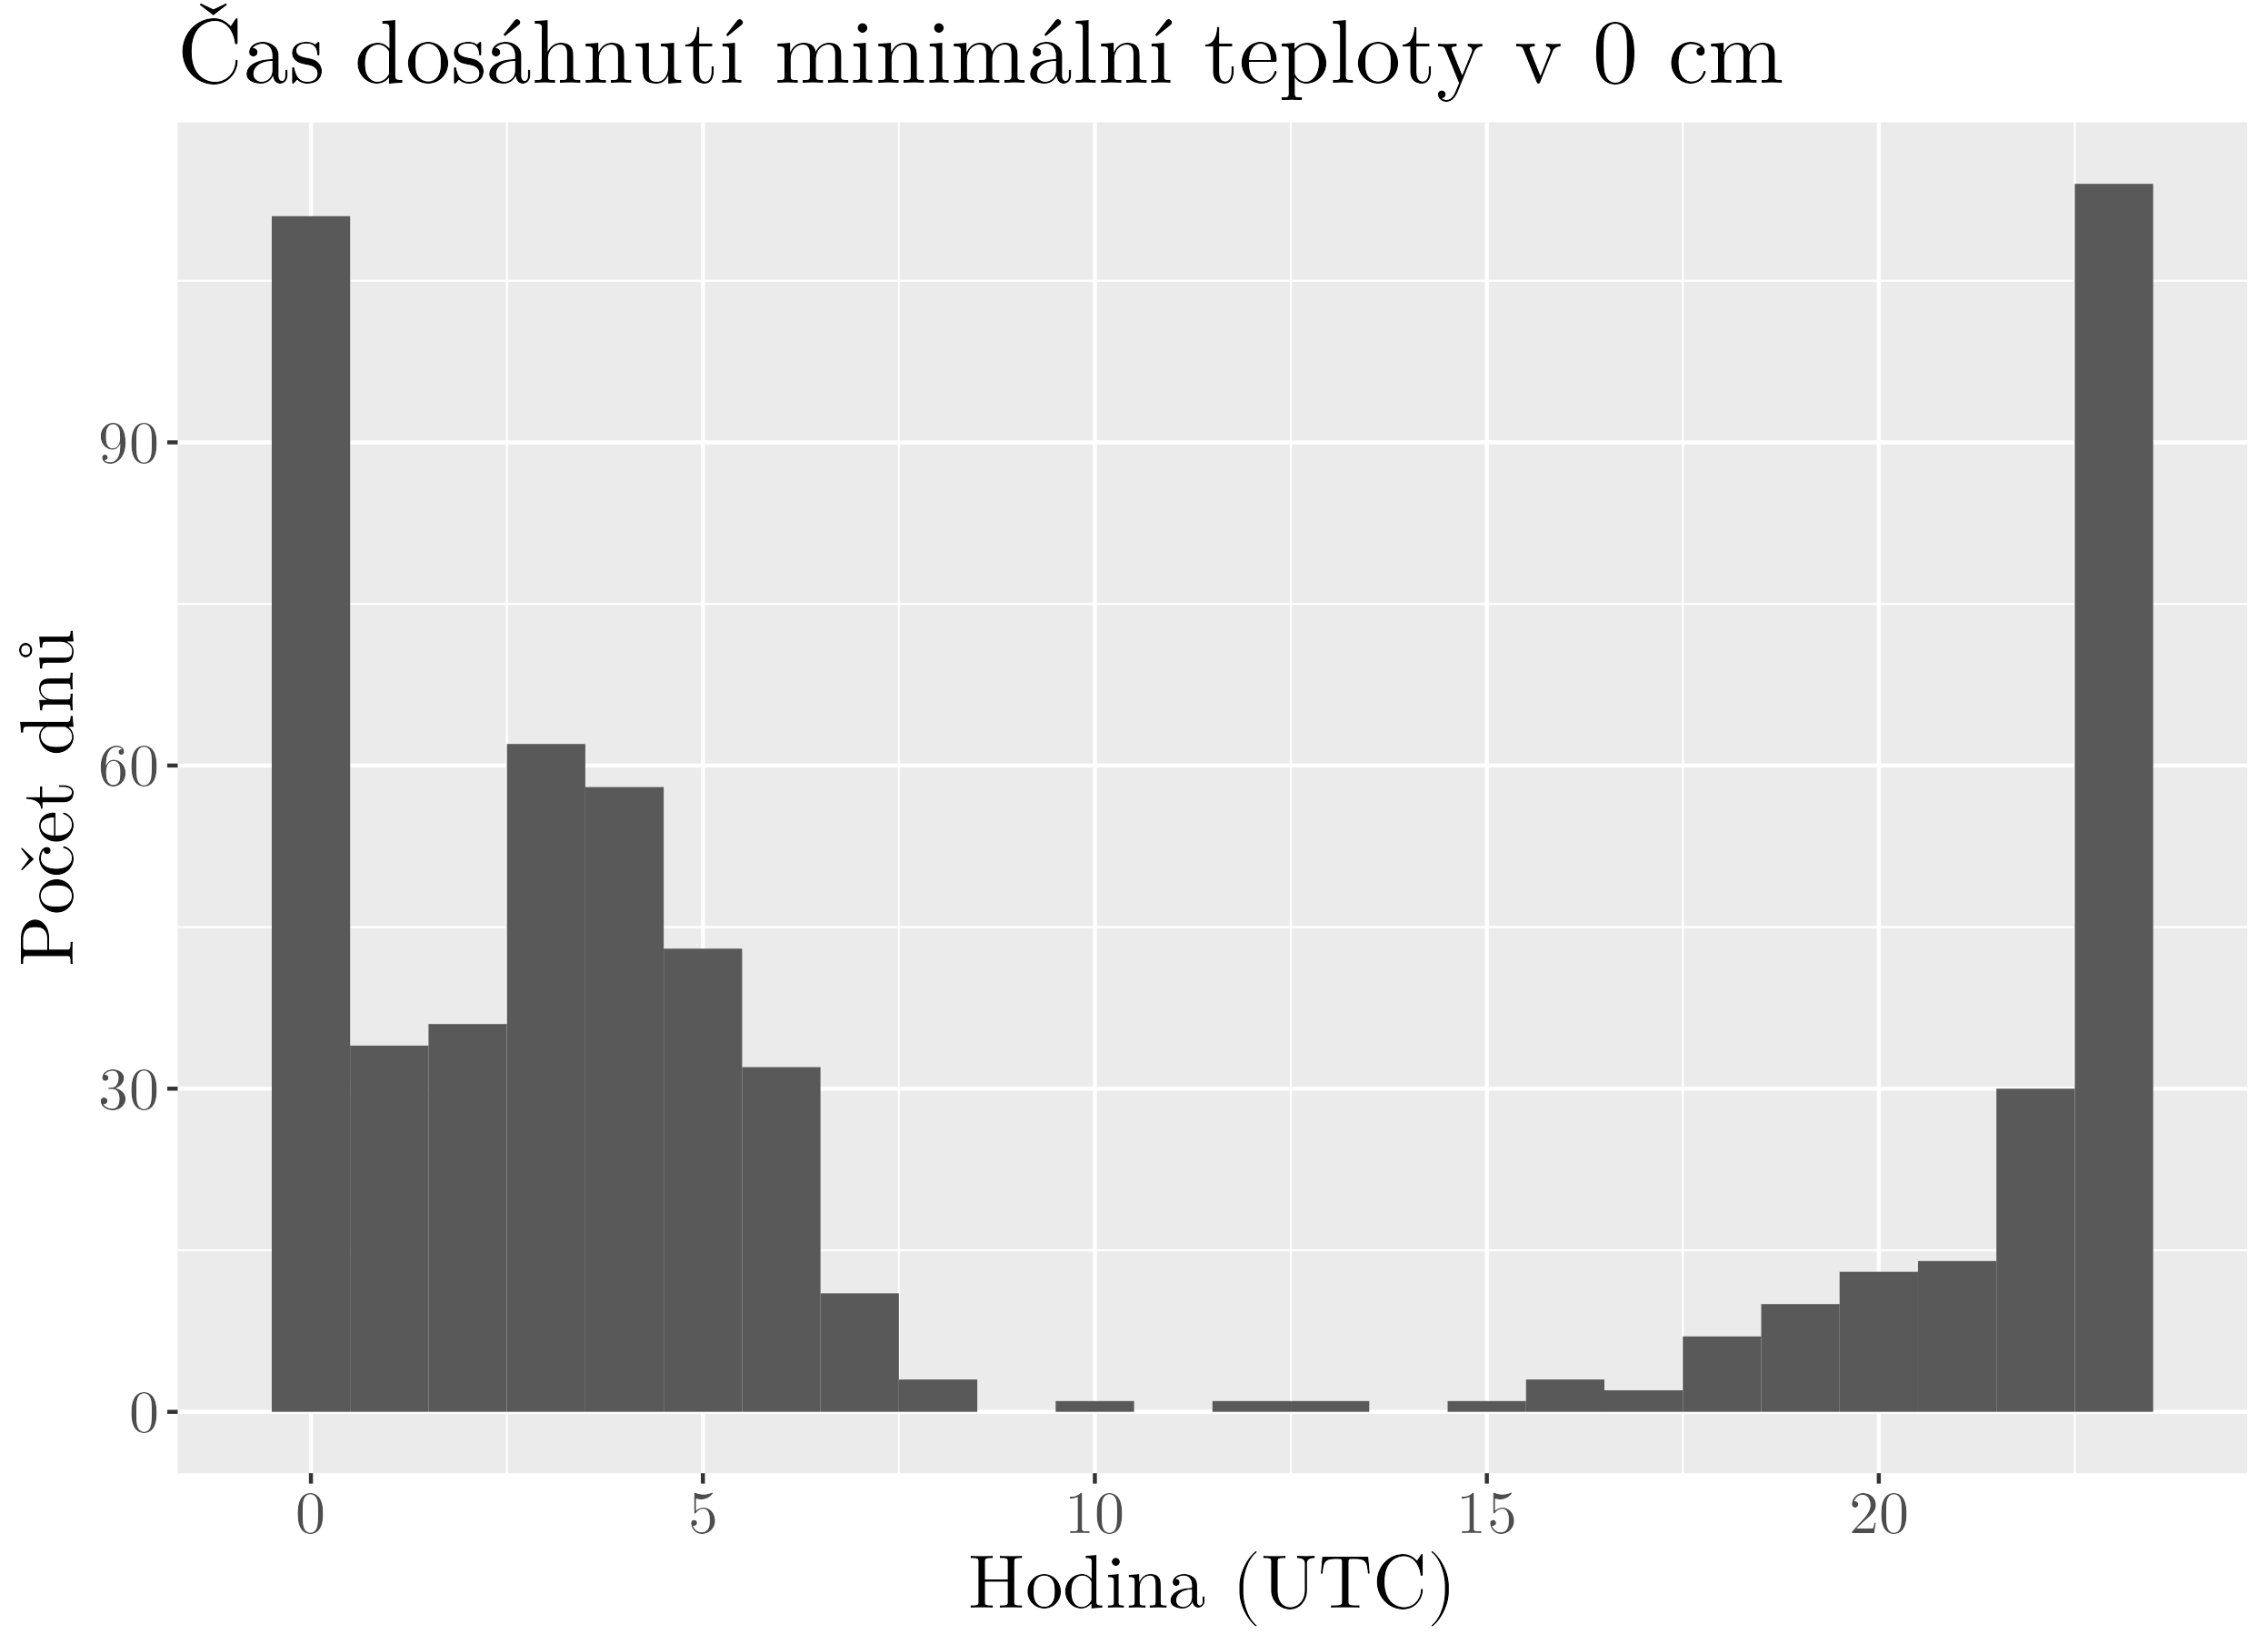
\includegraphics[width=\textwidth]{img/hist_hourmin0cm.png}
		\caption{}
		\label{fig:hourmin0cm}
	\end{subfigure}
	\caption{Denní doba (UTC) dosažení maximální resp. minimální teploty v $\SI{15}{cm}$ resp. v $\SI{0}{cm}$ nad zemí na čidle nejblíže stanici Churáňov}
	\label{fig:hours}
\end{figure}

Pro ilustraci se podívejme na konkrétní hodnoty teplot pozorované na nejbližším čidlu meteorologické stanice Churáňov. Na obrázcích \ref{fig:maxtemp} můžeme vidět průběh denních minim a maxim na jednom z čidel, celkově jde o období od 12.10.2019 do 20.5.2021 tedy 587 dnů. Na obrázcích \ref{fig:2mhours} můžeme vidět obrázkům \ref{fig:hourmax15cm} a \ref{fig:hourmin15cm} odpovídající hodnoty teplot naměřených ve výšce $\SI{2}{m}$ na čidle zavěšeném na stromě poblíž pozemním čidlům.

\begin{figure}
	\centering
	\begin{subfigure}{0.45\textwidth}
  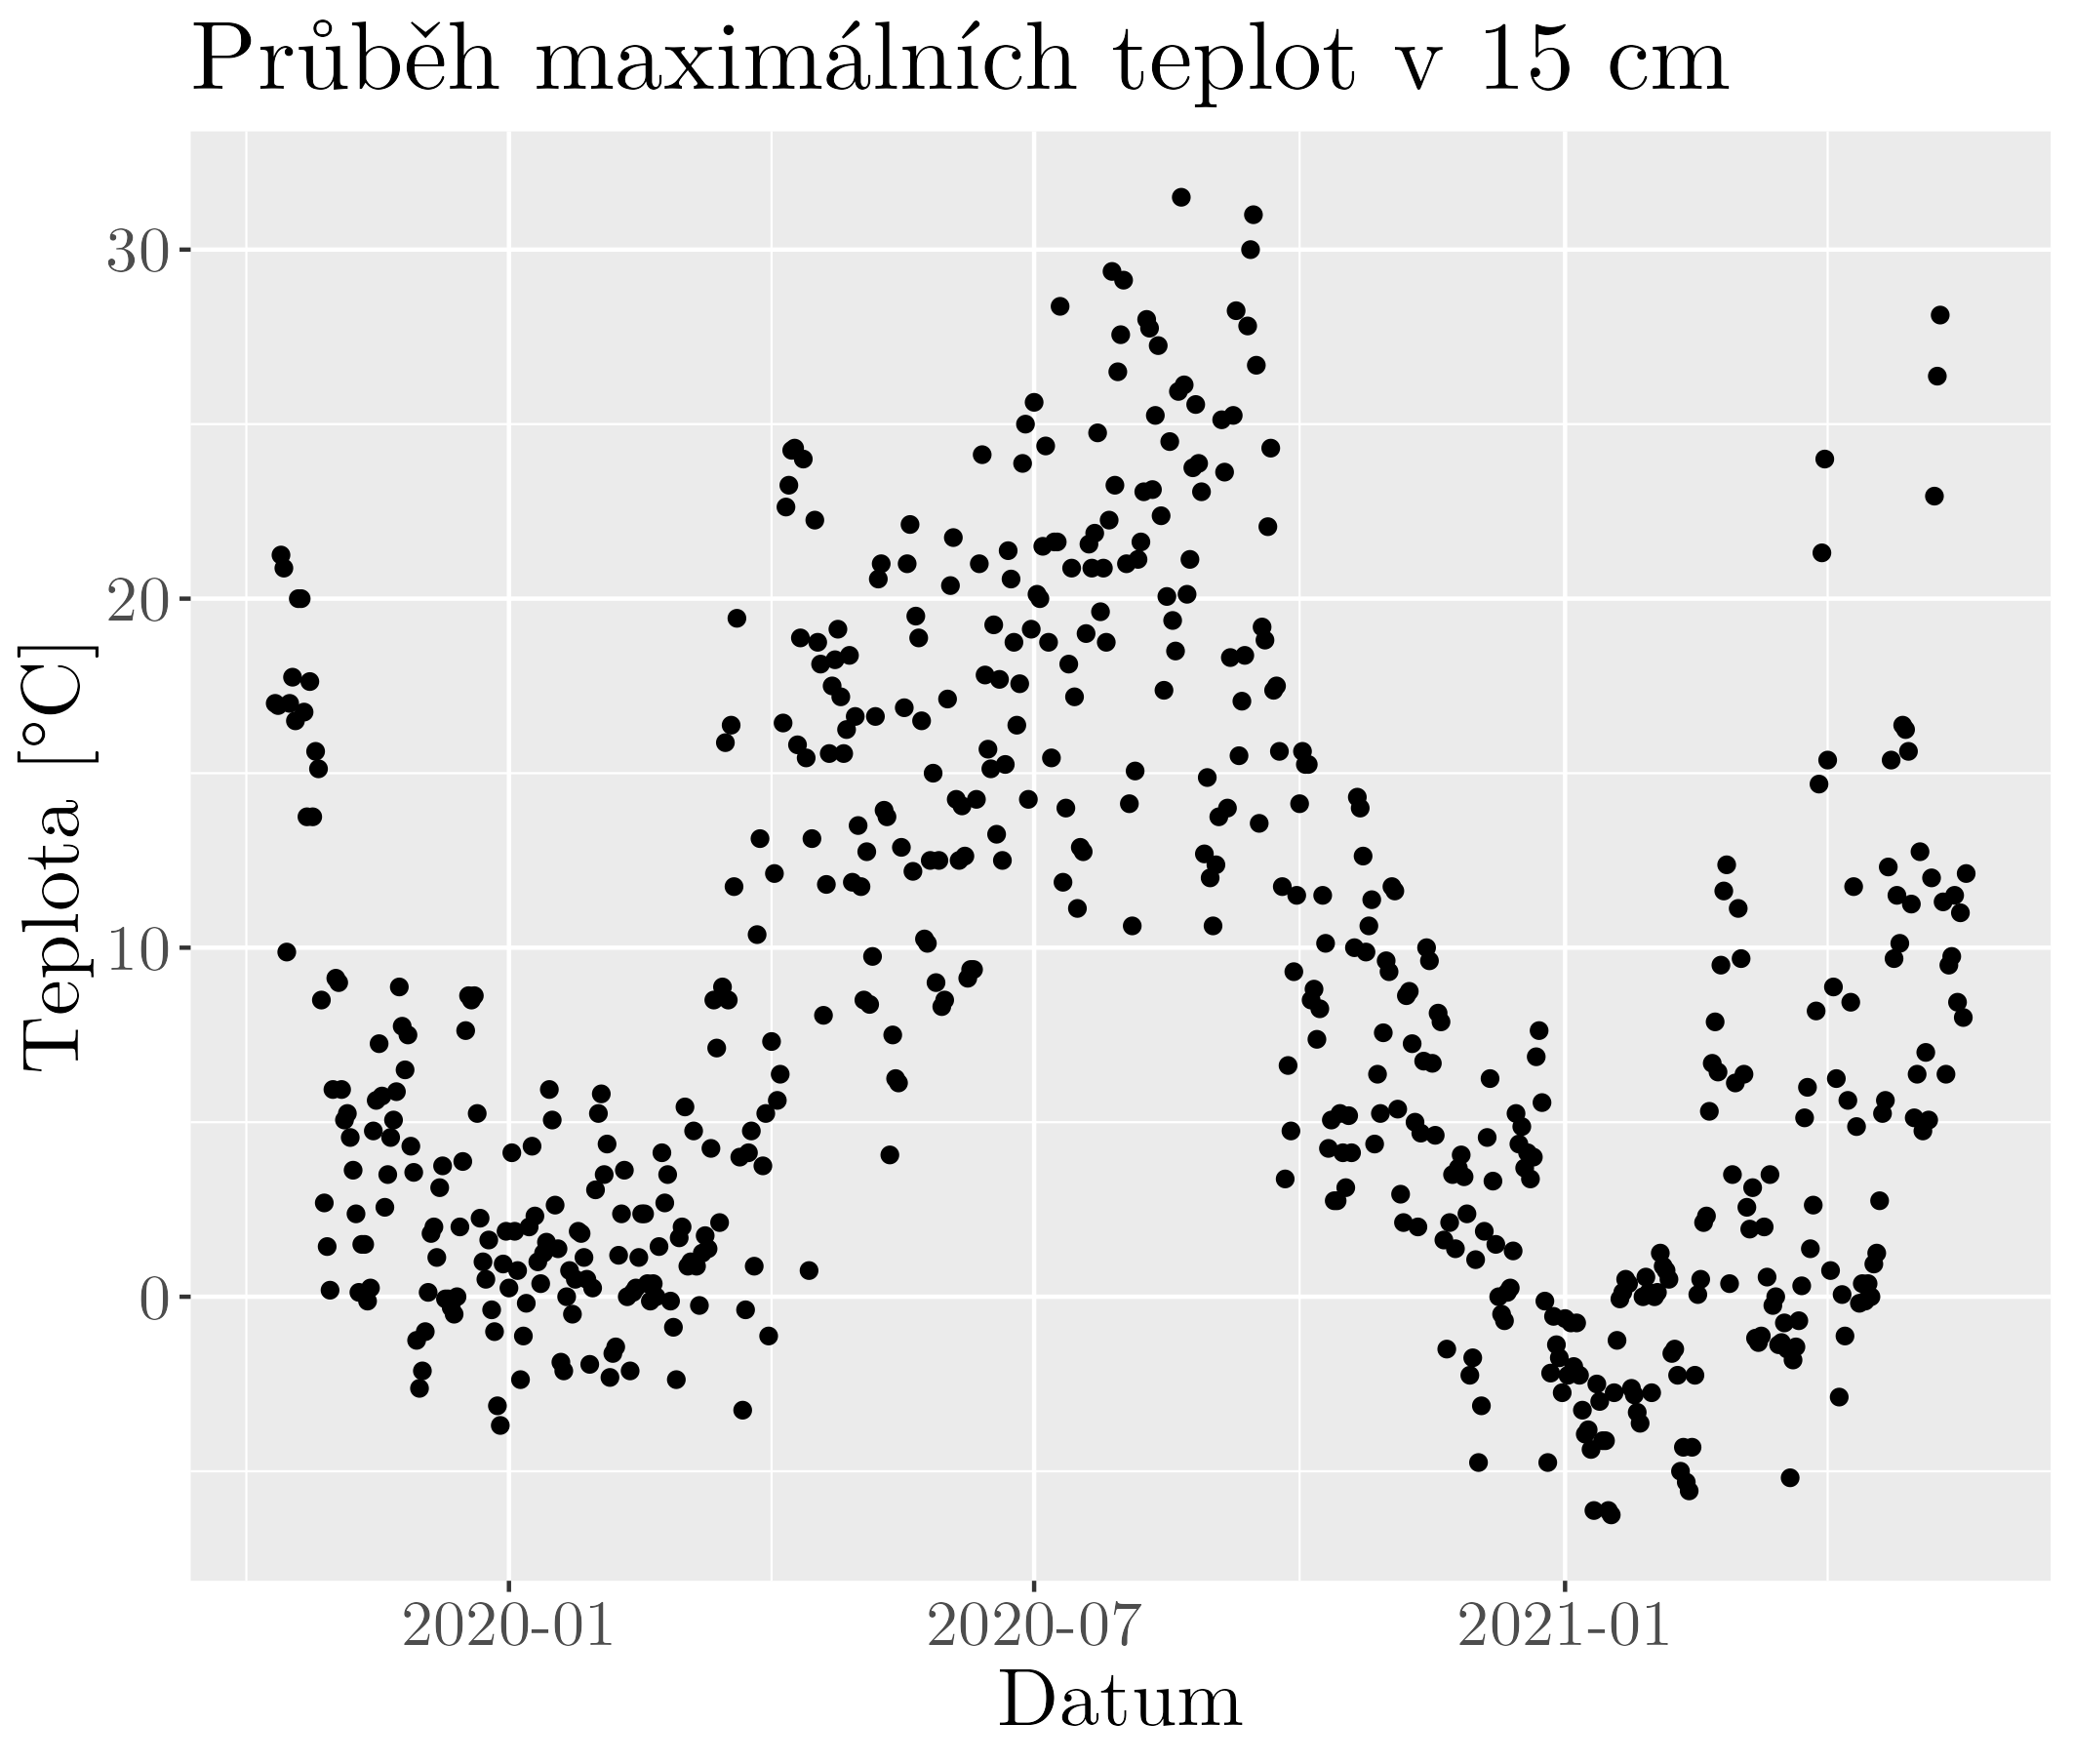
\includegraphics[width=\textwidth]{img/maxtempmax15cm.png}
		\caption{}
		\label{fig:maxtempmax15cm}
	\end{subfigure}
	\hfill
	\begin{subfigure}{0.45\textwidth}
  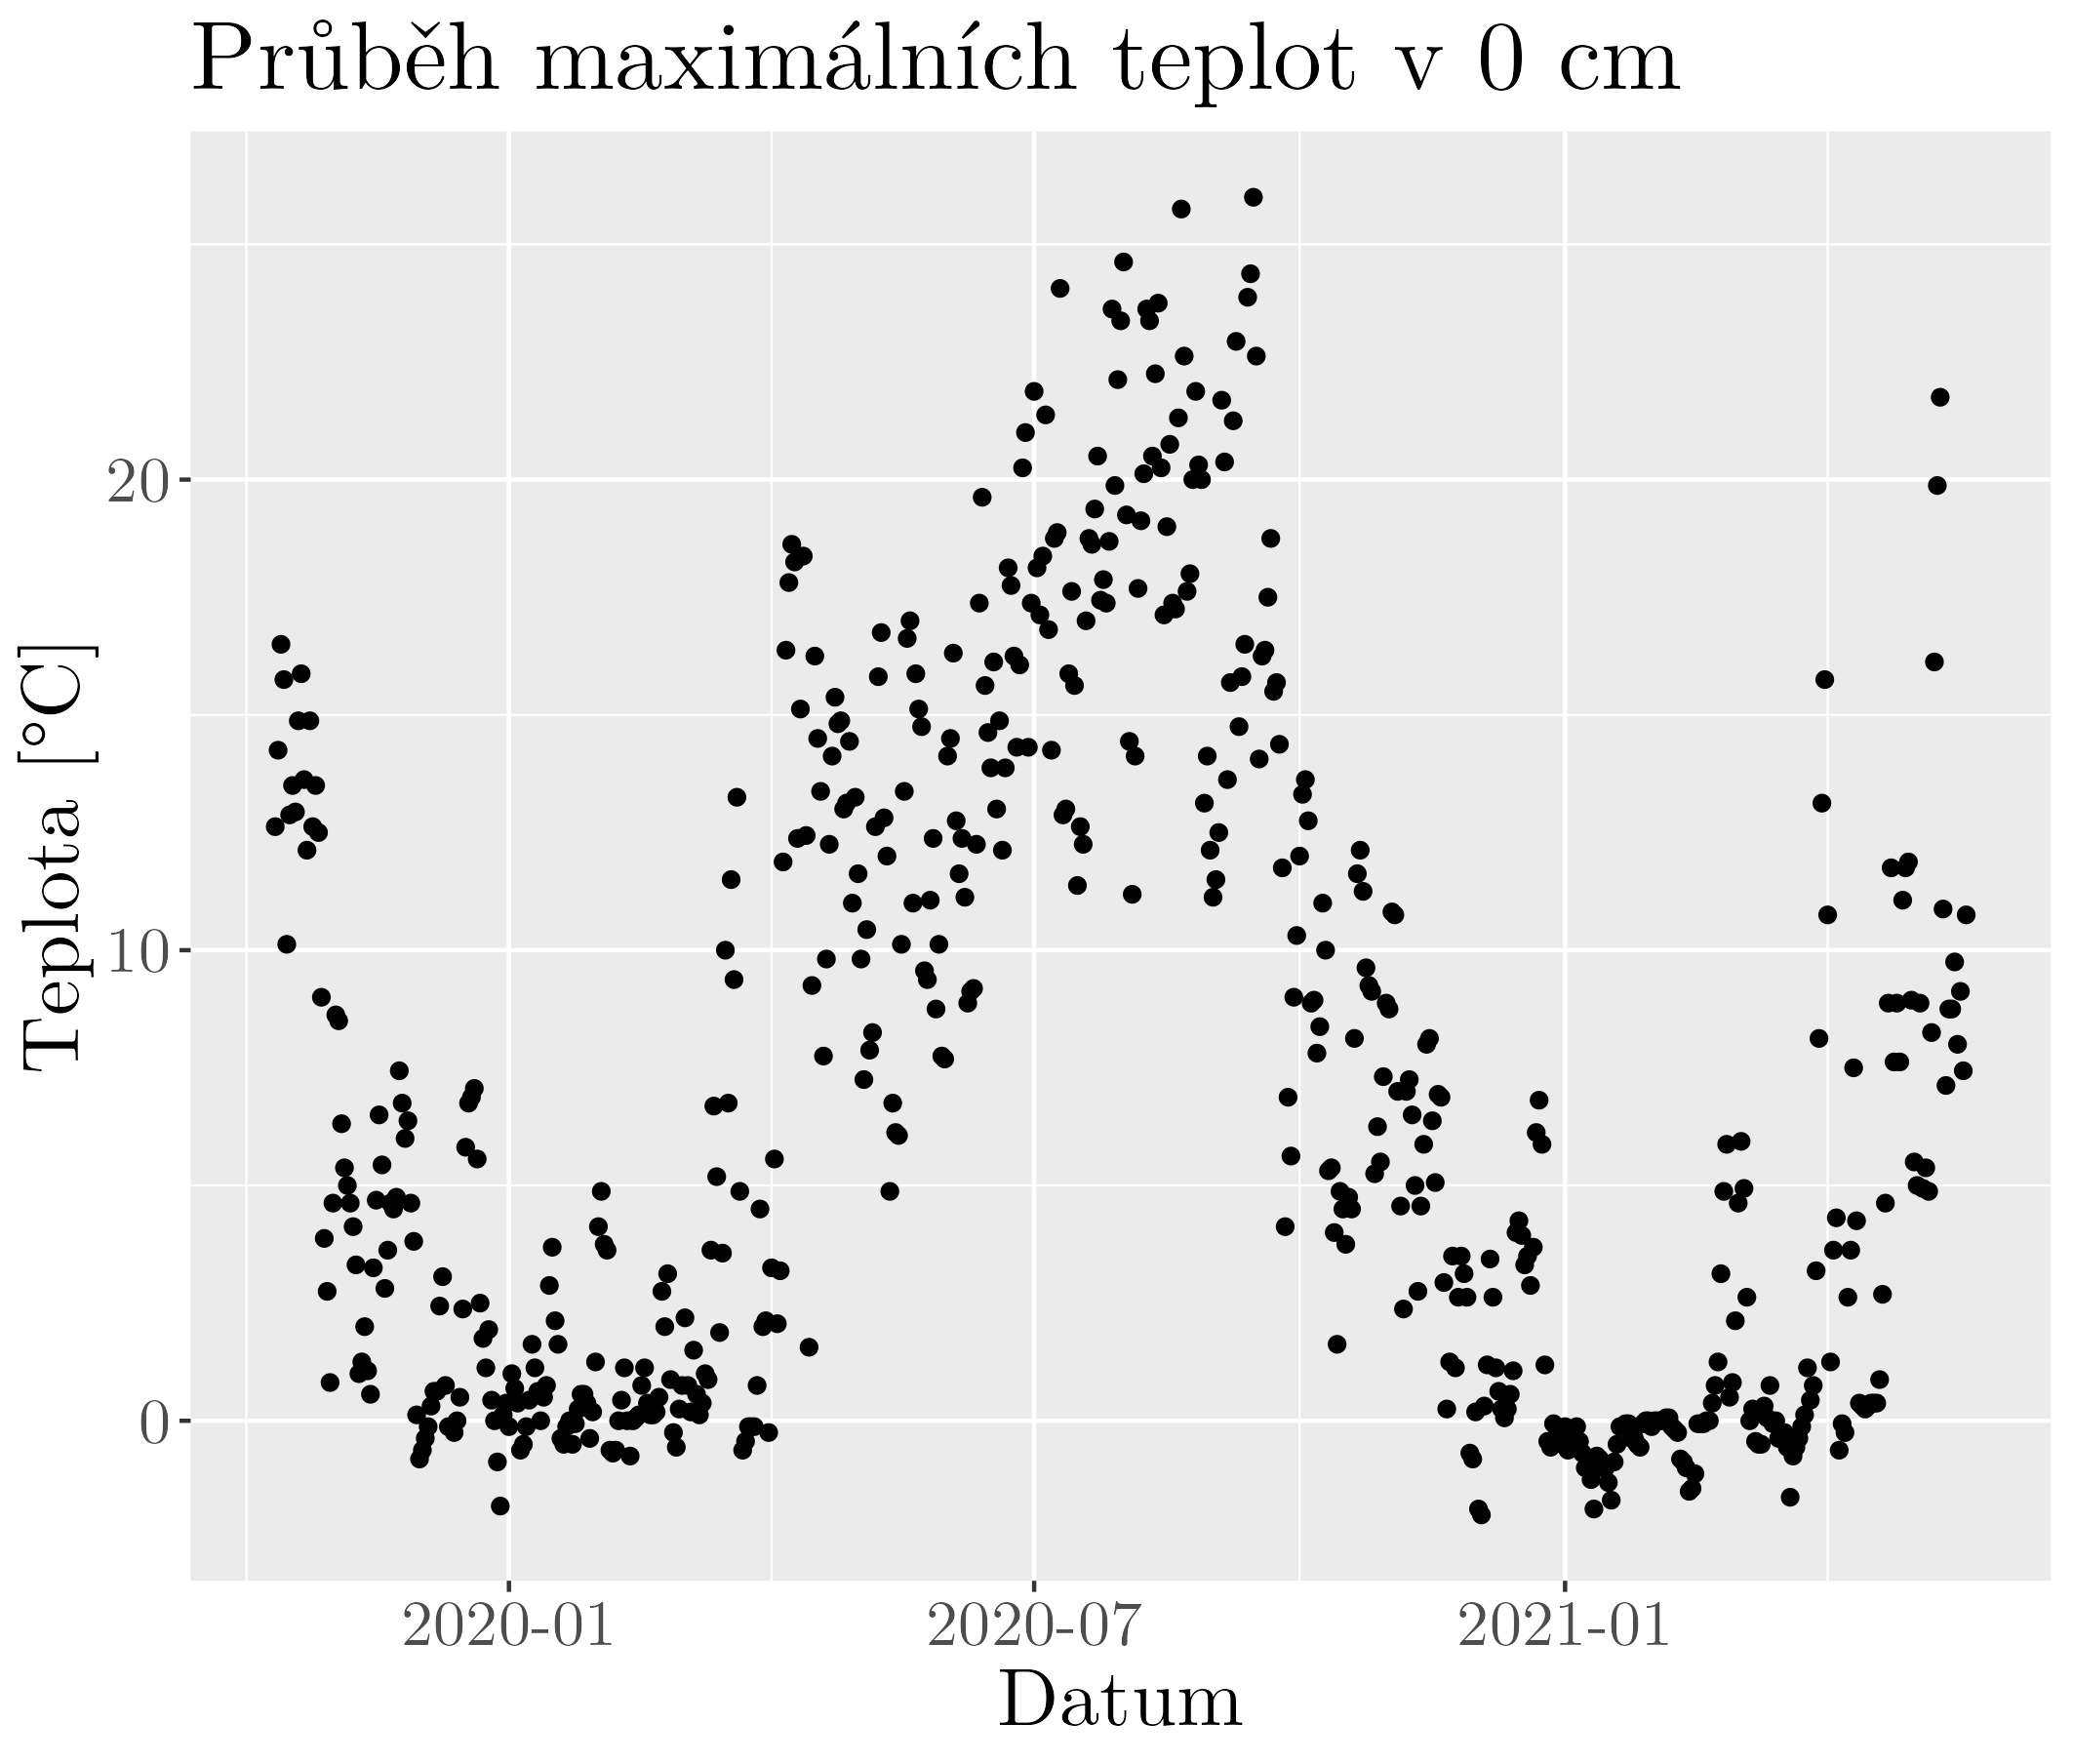
\includegraphics[width=\textwidth]{img/maxtempmax0cm.png}
		\caption{}
		\label{fig:maxtempmax0cm}
	\end{subfigure}
	\hfill
	\begin{subfigure}{0.45\textwidth}
  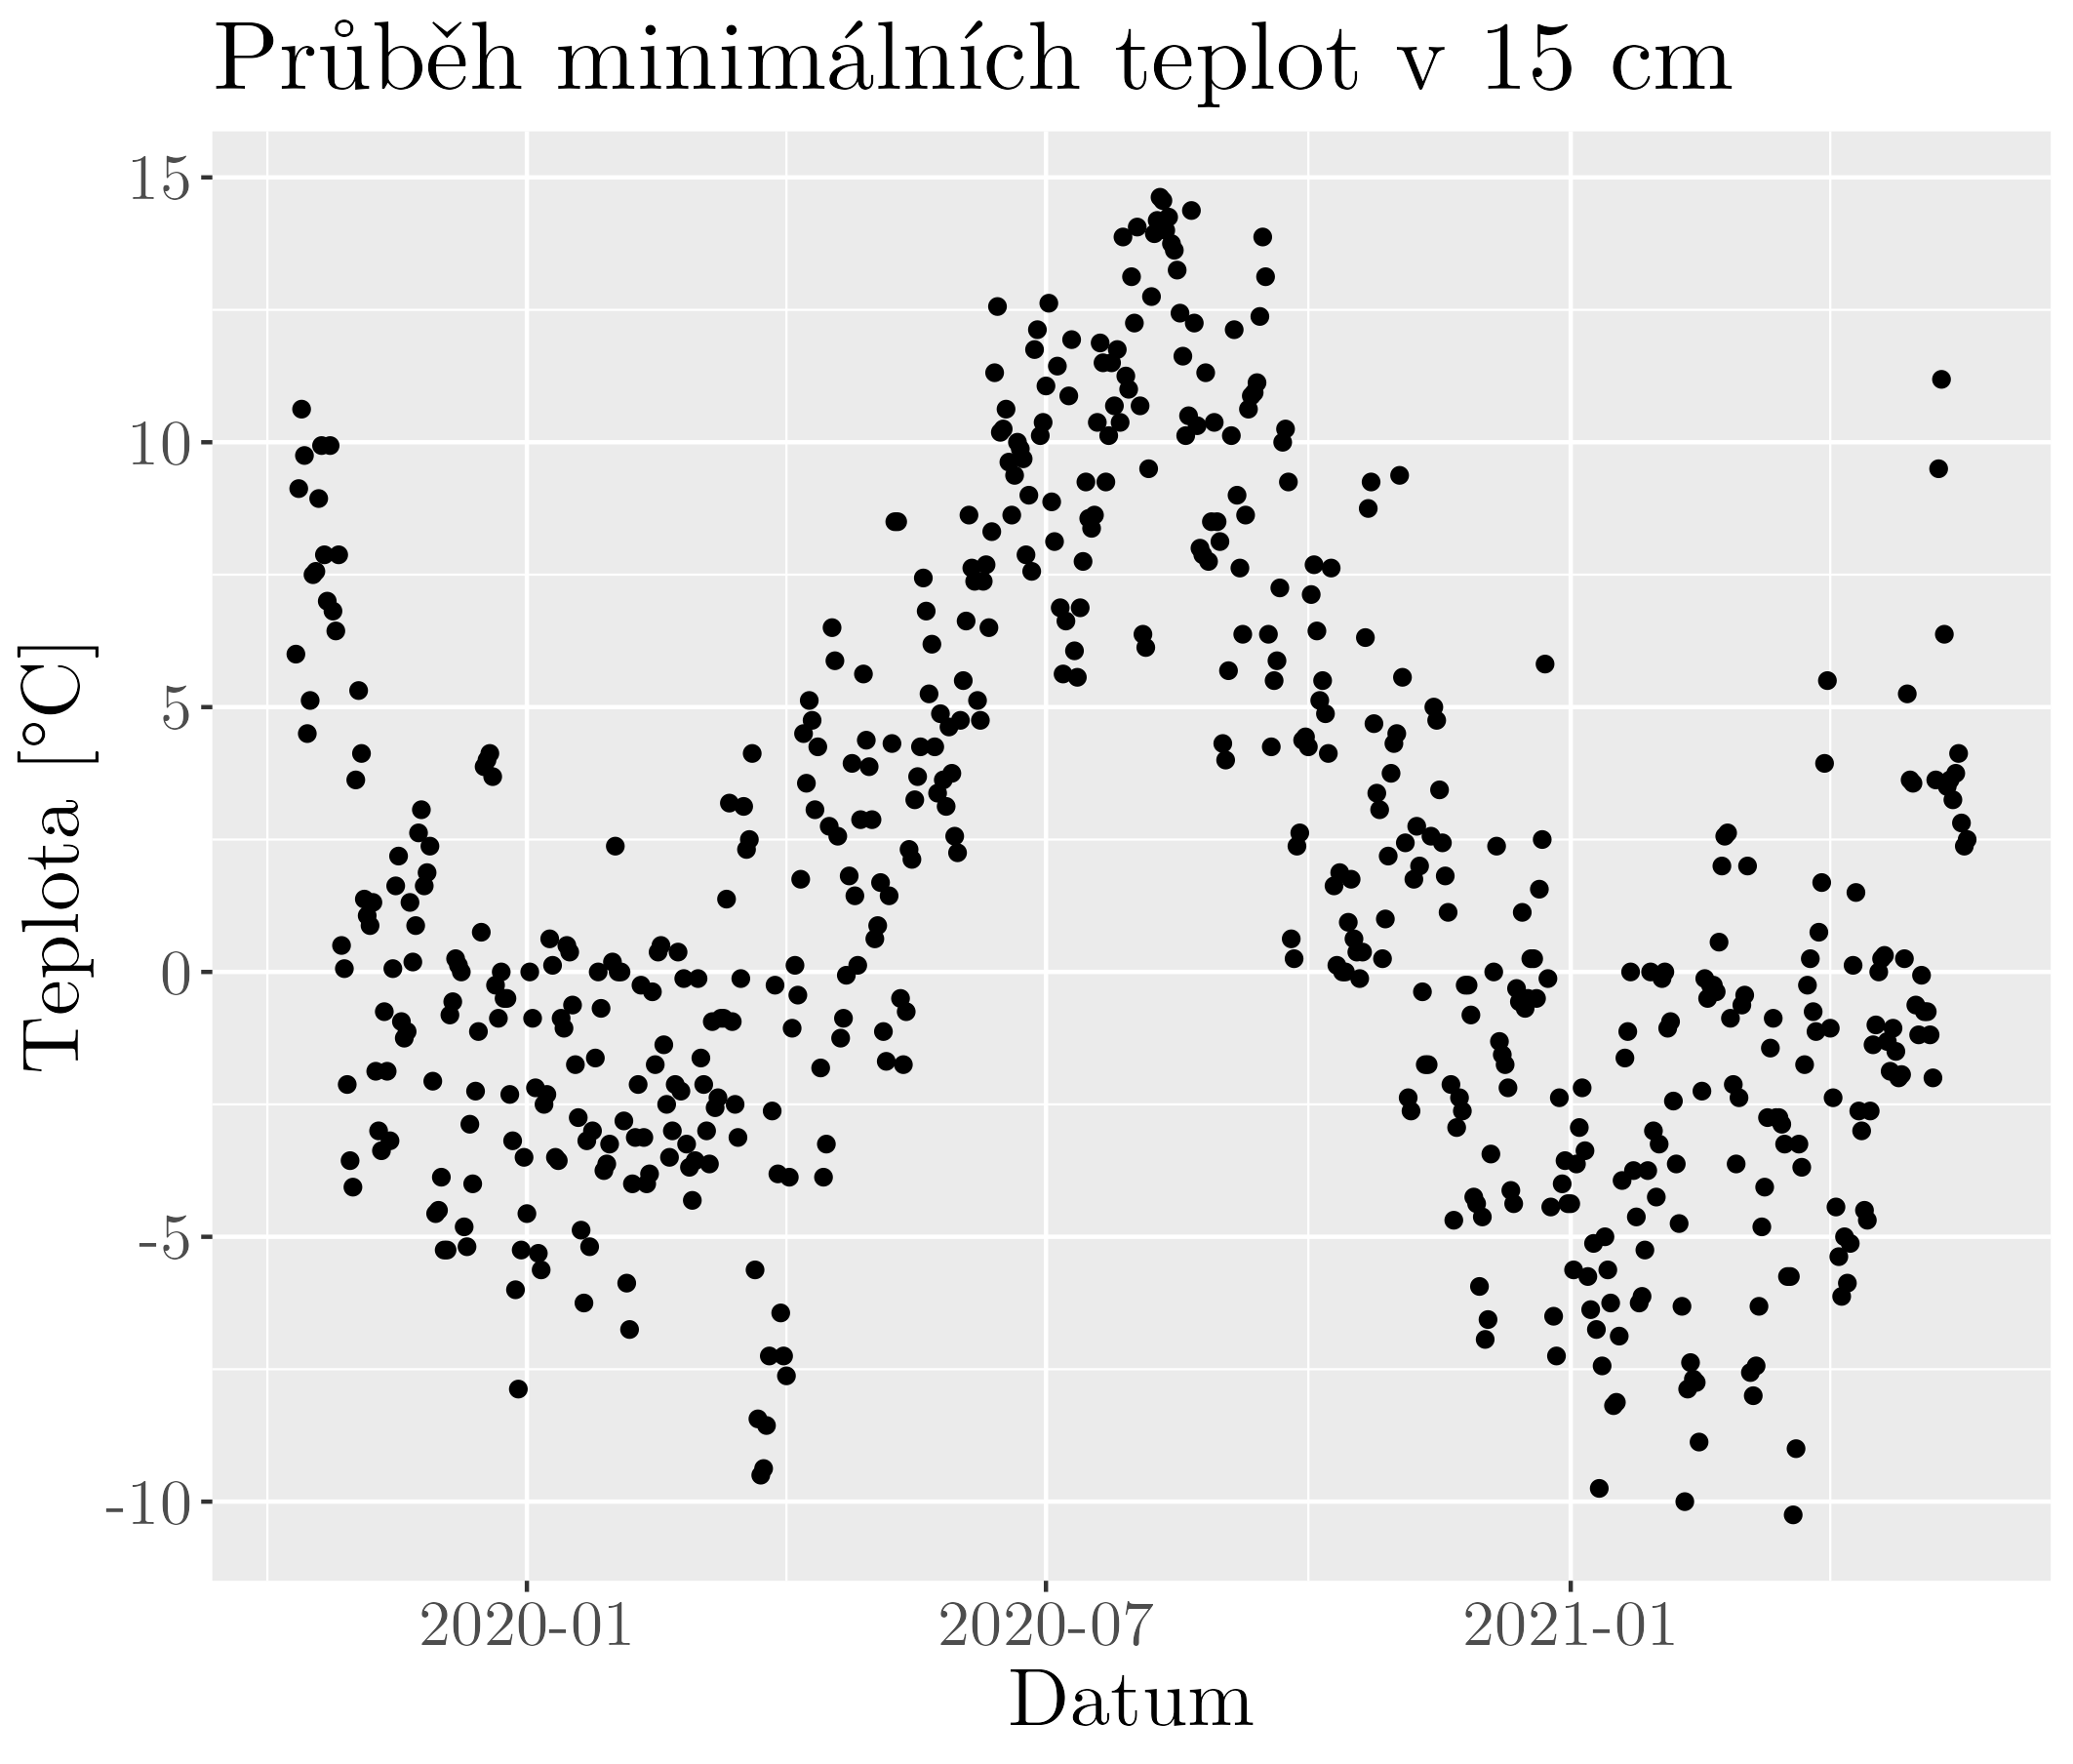
\includegraphics[width=\textwidth]{img/maxtempmin15cm.png}
		\caption{}
		\label{fig:maxtempmin15cm}
	\end{subfigure}
	\hfill
	\begin{subfigure}{0.45\textwidth}
  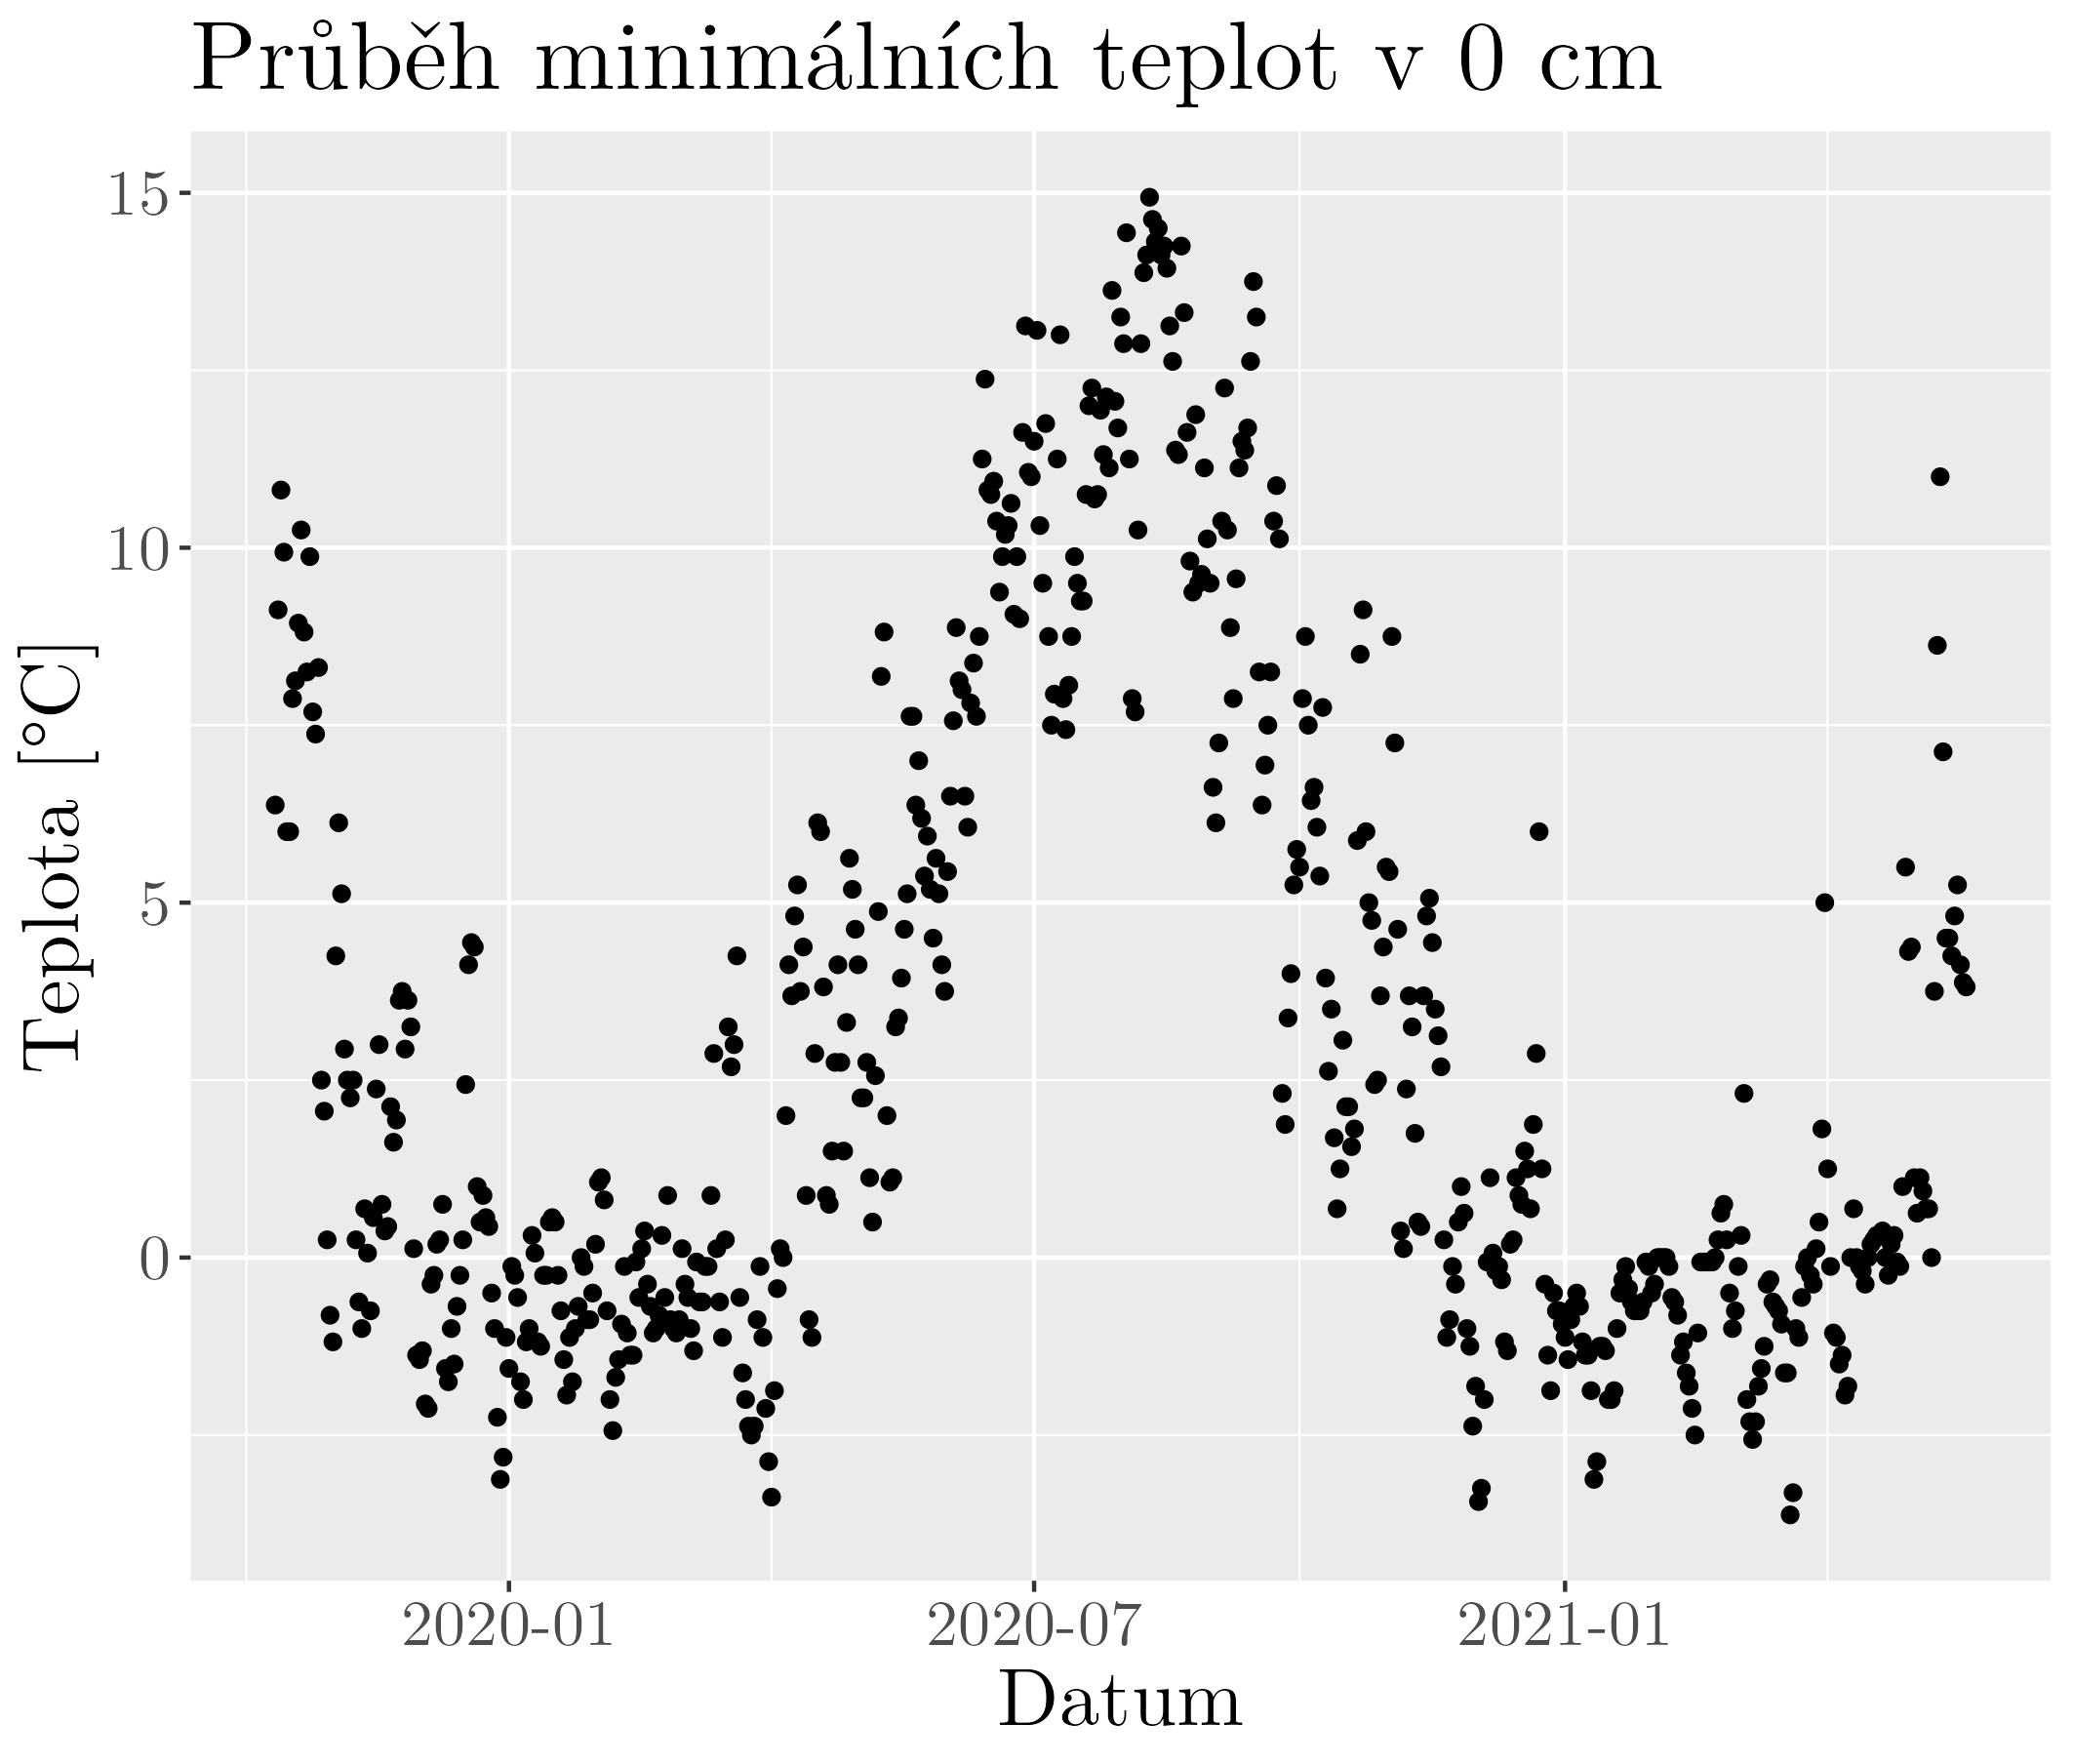
\includegraphics[width=\textwidth]{img/maxtempmin0cm.png}
		\caption{}
		\label{fig:maxtempmin0cm}
	\end{subfigure}
	\caption{Průběh denních maximální resp. minimálních teplot ve výšce $\SI{15}{cm}$ resp. $\SI{0}{cm}$ nad zemí na čidle nejblíže stanici Churáňov}
	\label{fig:maxtemp}
\end{figure}

\begin{figure}
	\centering
	\begin{subfigure}{0.45\textwidth}
  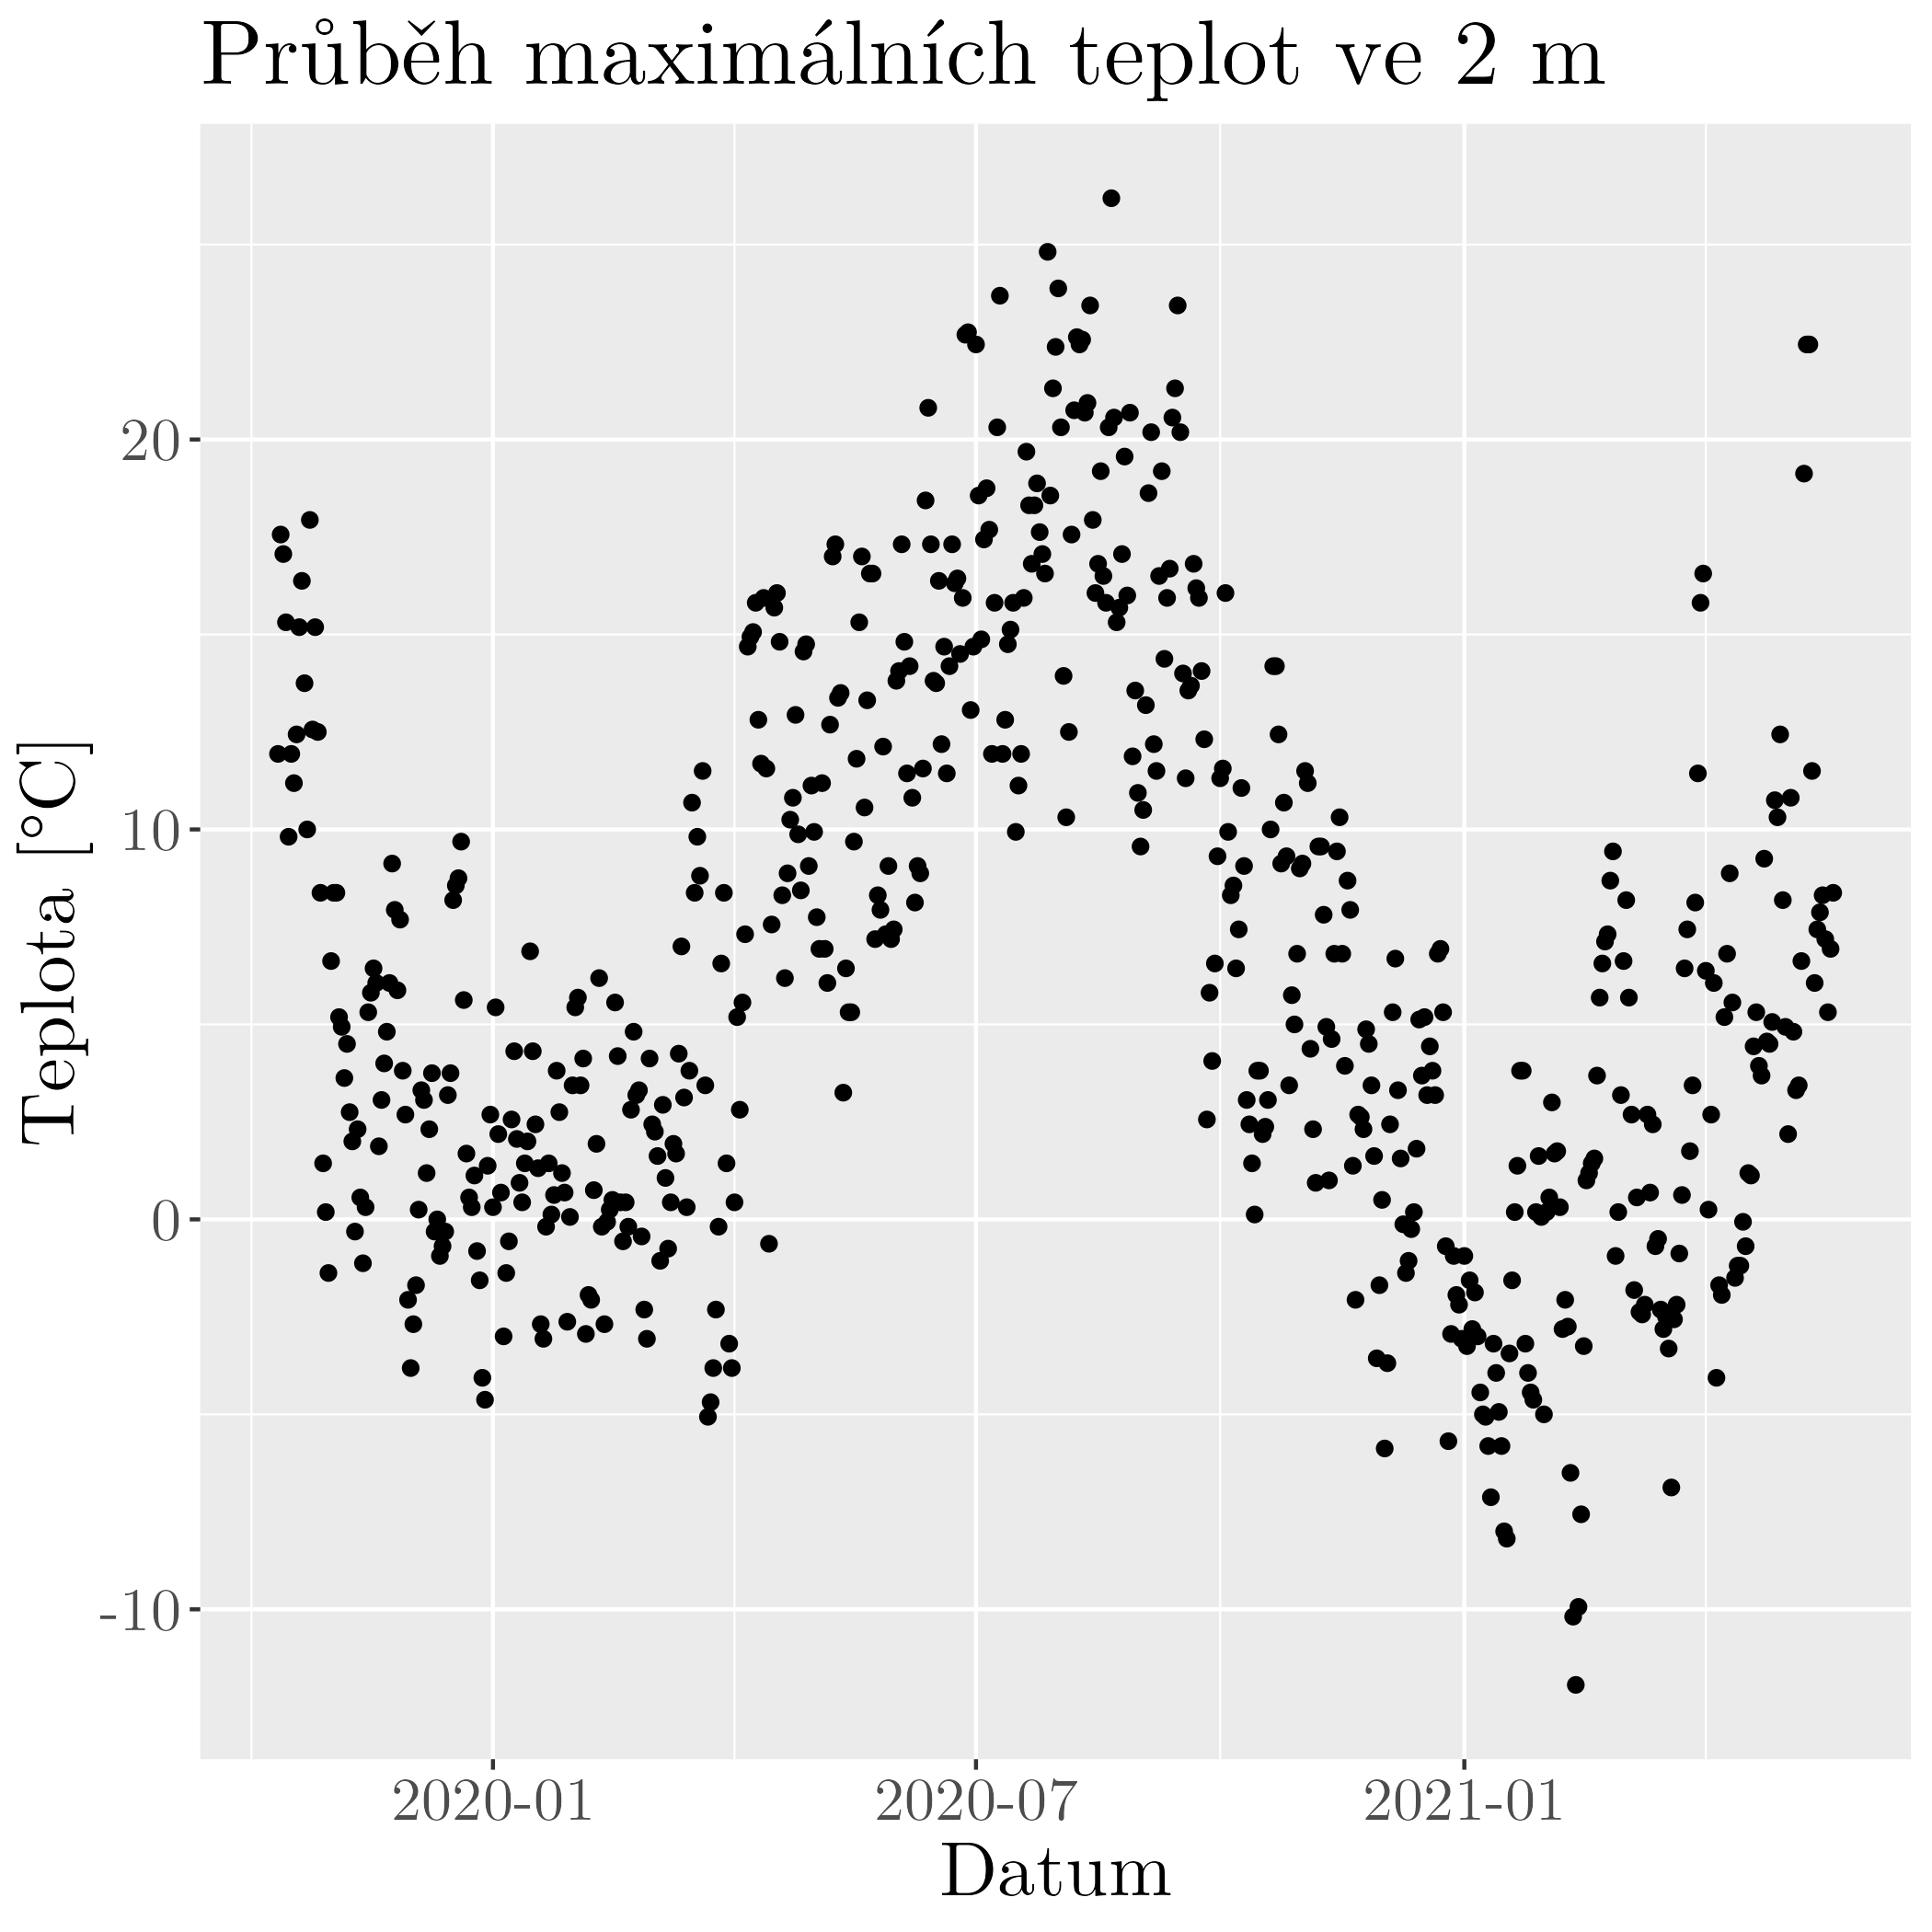
\includegraphics[width=\textwidth]{img/2mmaxtempmax15cm.png}
		\caption{Teploty naměřené ve stejnou dobu jako maximální teploty v $\SI{15}{cm}$}
		\label{fig:2mmaxtempmax15cm}
	\end{subfigure}
	\hfill
	\begin{subfigure}{0.45\textwidth}
  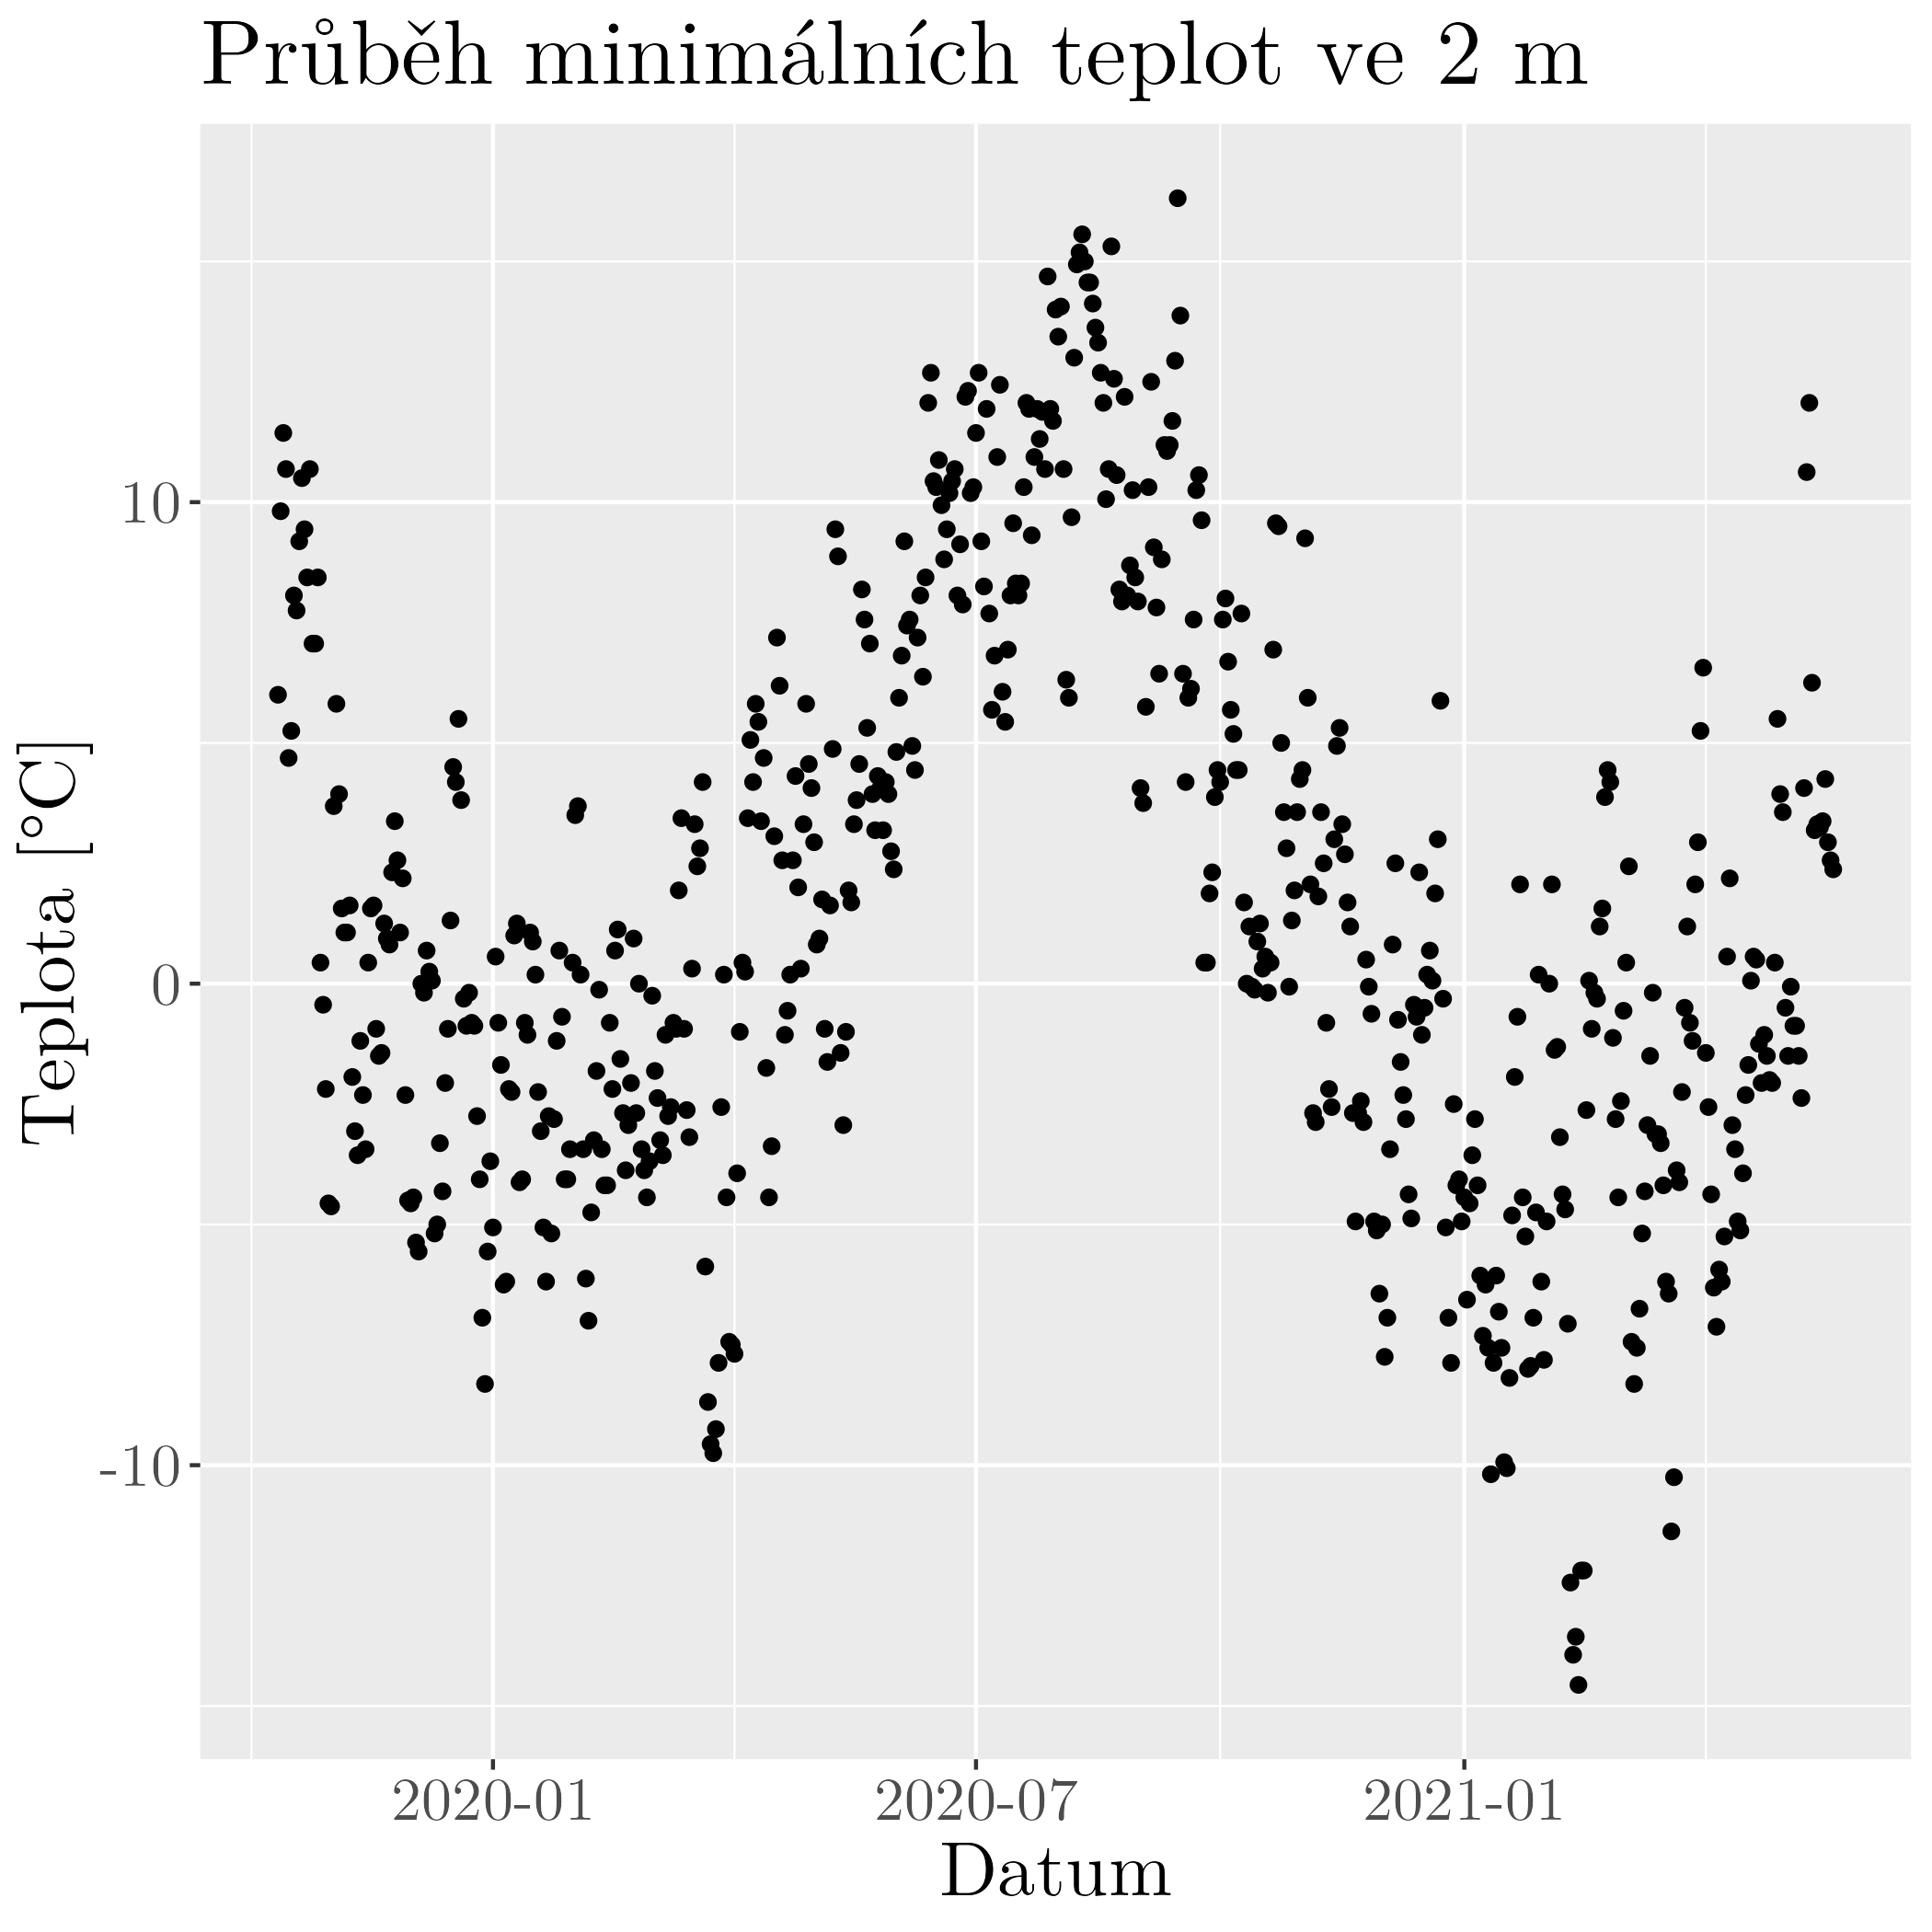
\includegraphics[width=\textwidth]{img/2mmaxtempmin15cm.png}
		\caption{Teploty naměřené ve stejnou dobu jako minimální teploty v $\SI{15}{cm}$}
		\label{fig:2mmaxtempmin15cm}
	\end{subfigure}
	\caption{Teploty ve výšce $\SI{2}{m}$ nad zemí na čidle nejblíže stanici Churáňov v době kdy nastalo maximum resp. minimum na čidle ve výšce $\SI{15}{cm}$}
	\label{fig:2mhours}
\end{figure}

Na obrázku \ref{fig:hist_diff} můžeme vidět histogramy rozdílů teplot pro jednotlivé výšky a pro maxima a minima.

\begin{figure}
	\centering
	\begin{subfigure}{0.45\textwidth}
  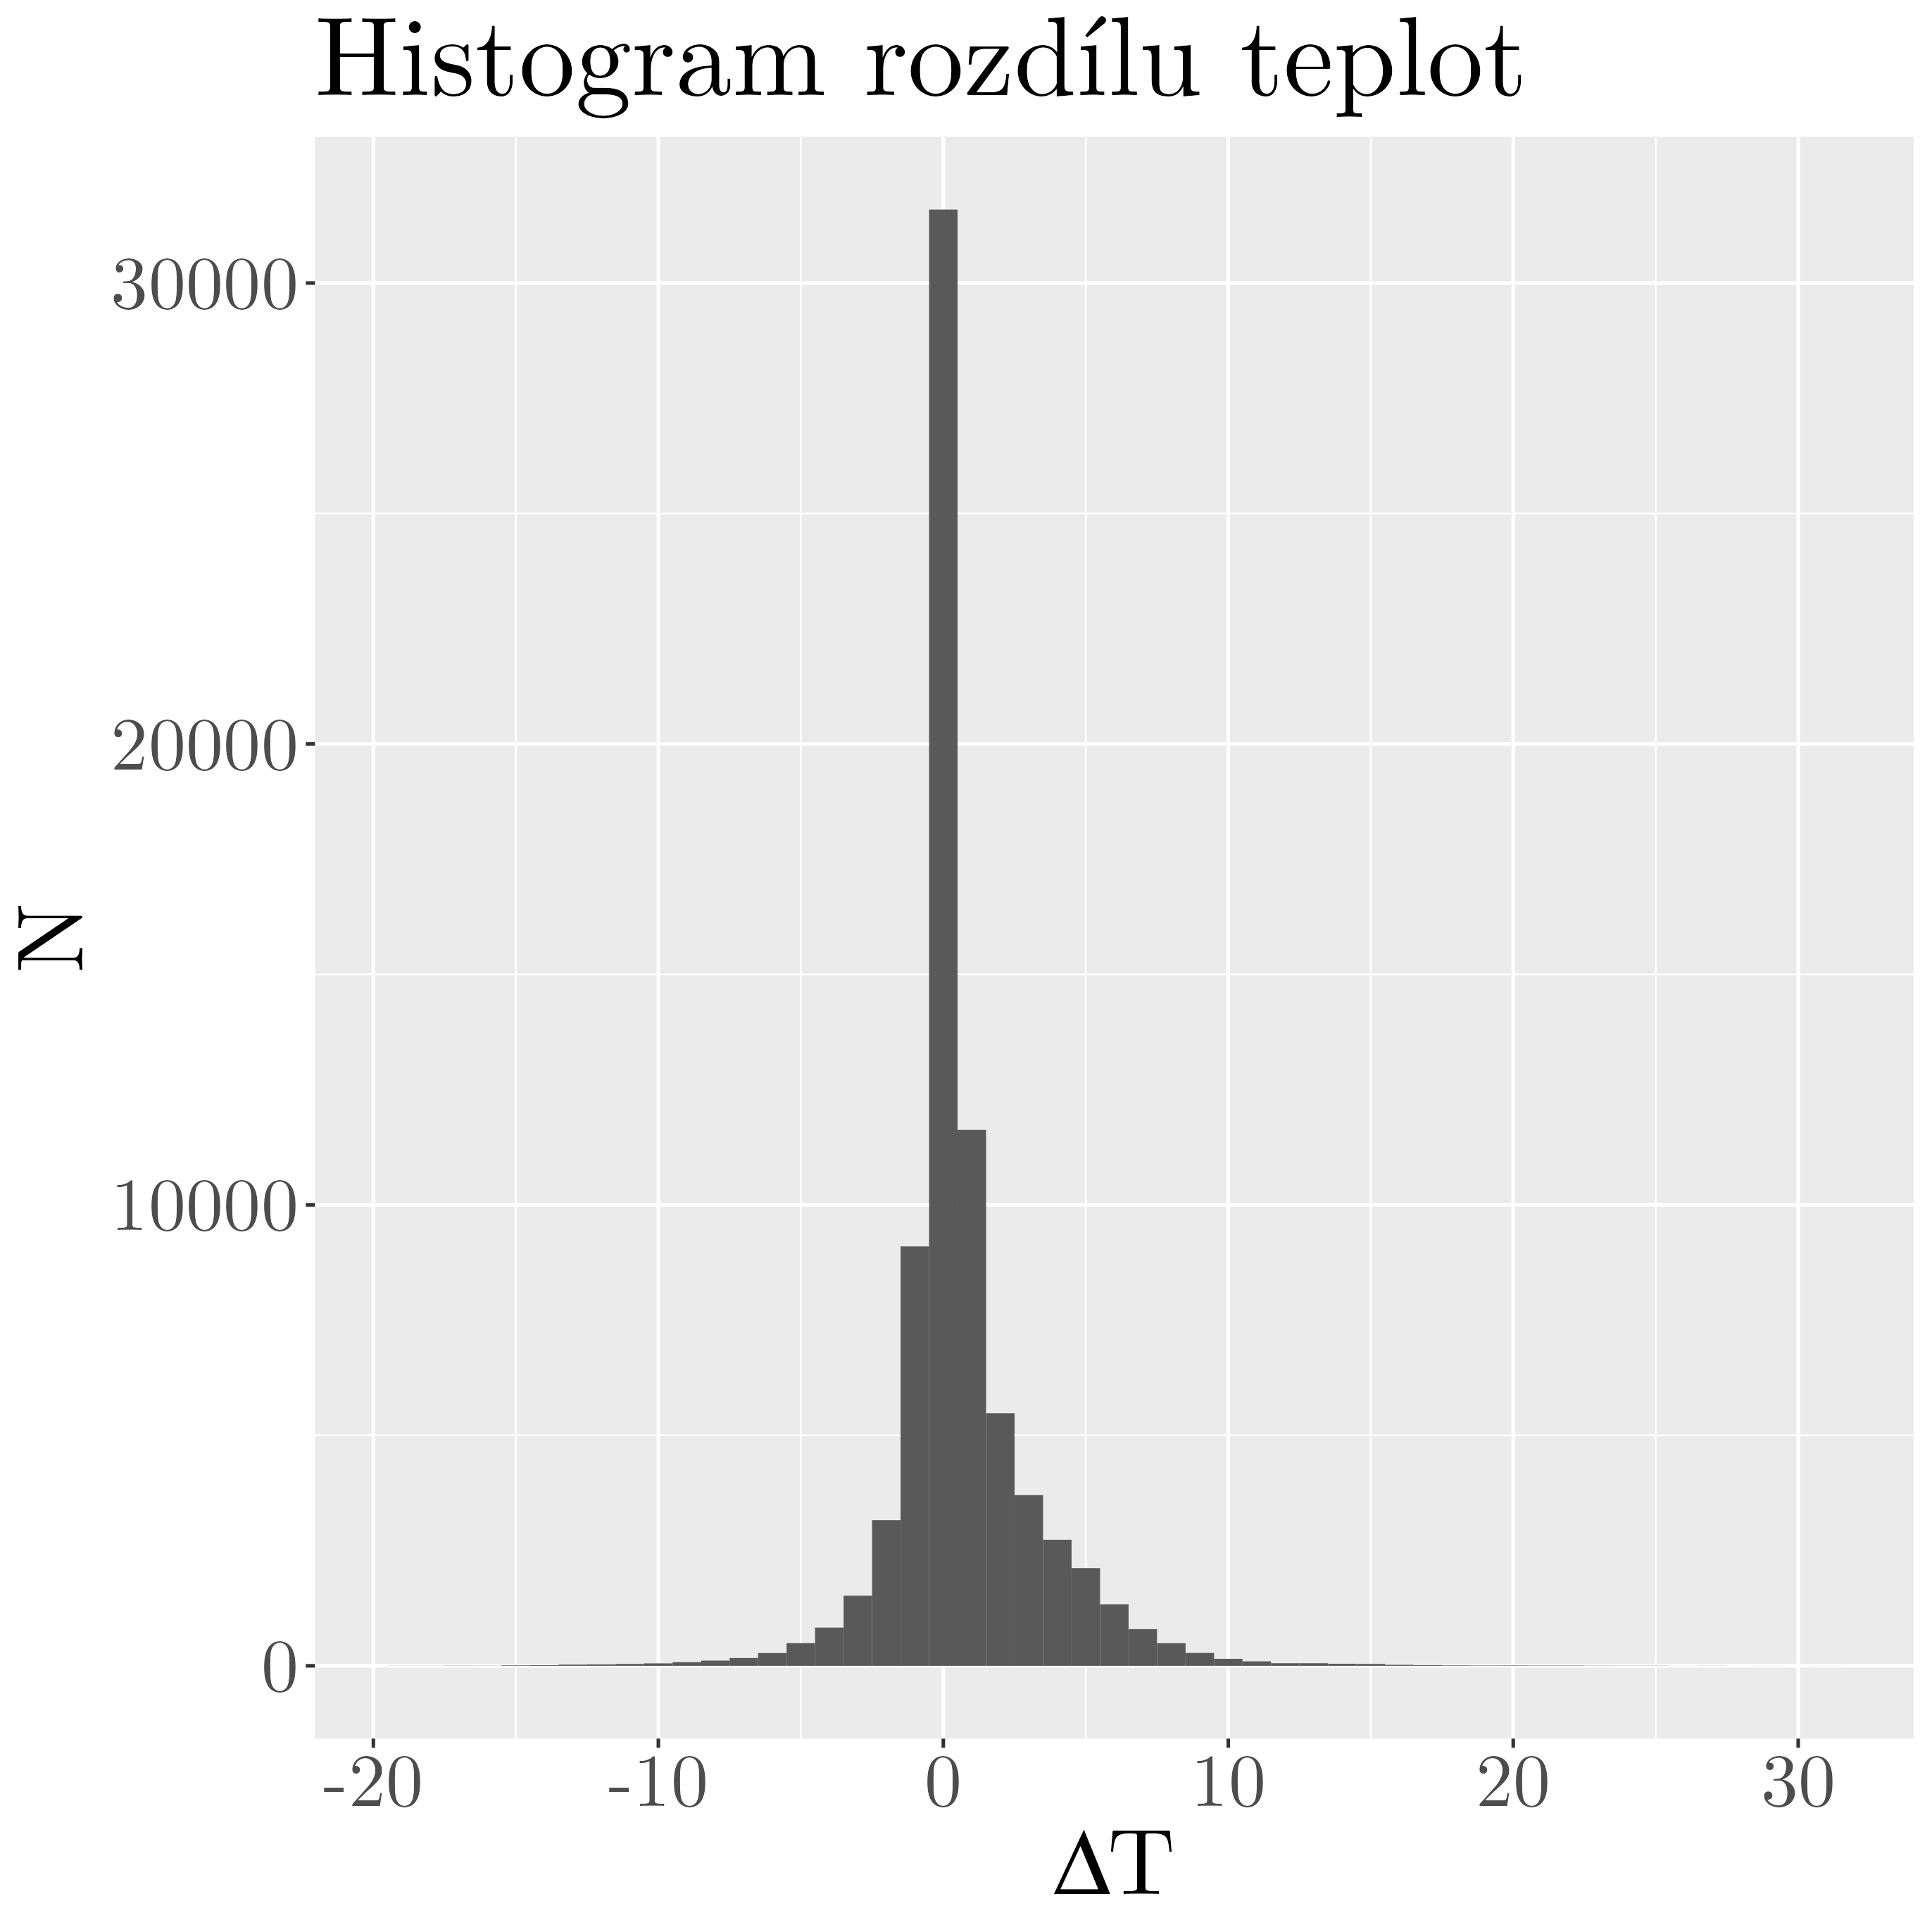
\includegraphics[width=\textwidth]{img/ch2/hist_diff_max15cm.png}
		\caption{Histogram rozdílu maximálních teplot v $\SI{15}{cm}$ a $\SI{2}{m}$. $\text{M} = 0.69$, $\text{MD} = 0.25$.}
		\label{fig:hist_diff_max15cm}
	\end{subfigure}
	\hfill
	\begin{subfigure}{0.45\textwidth}
  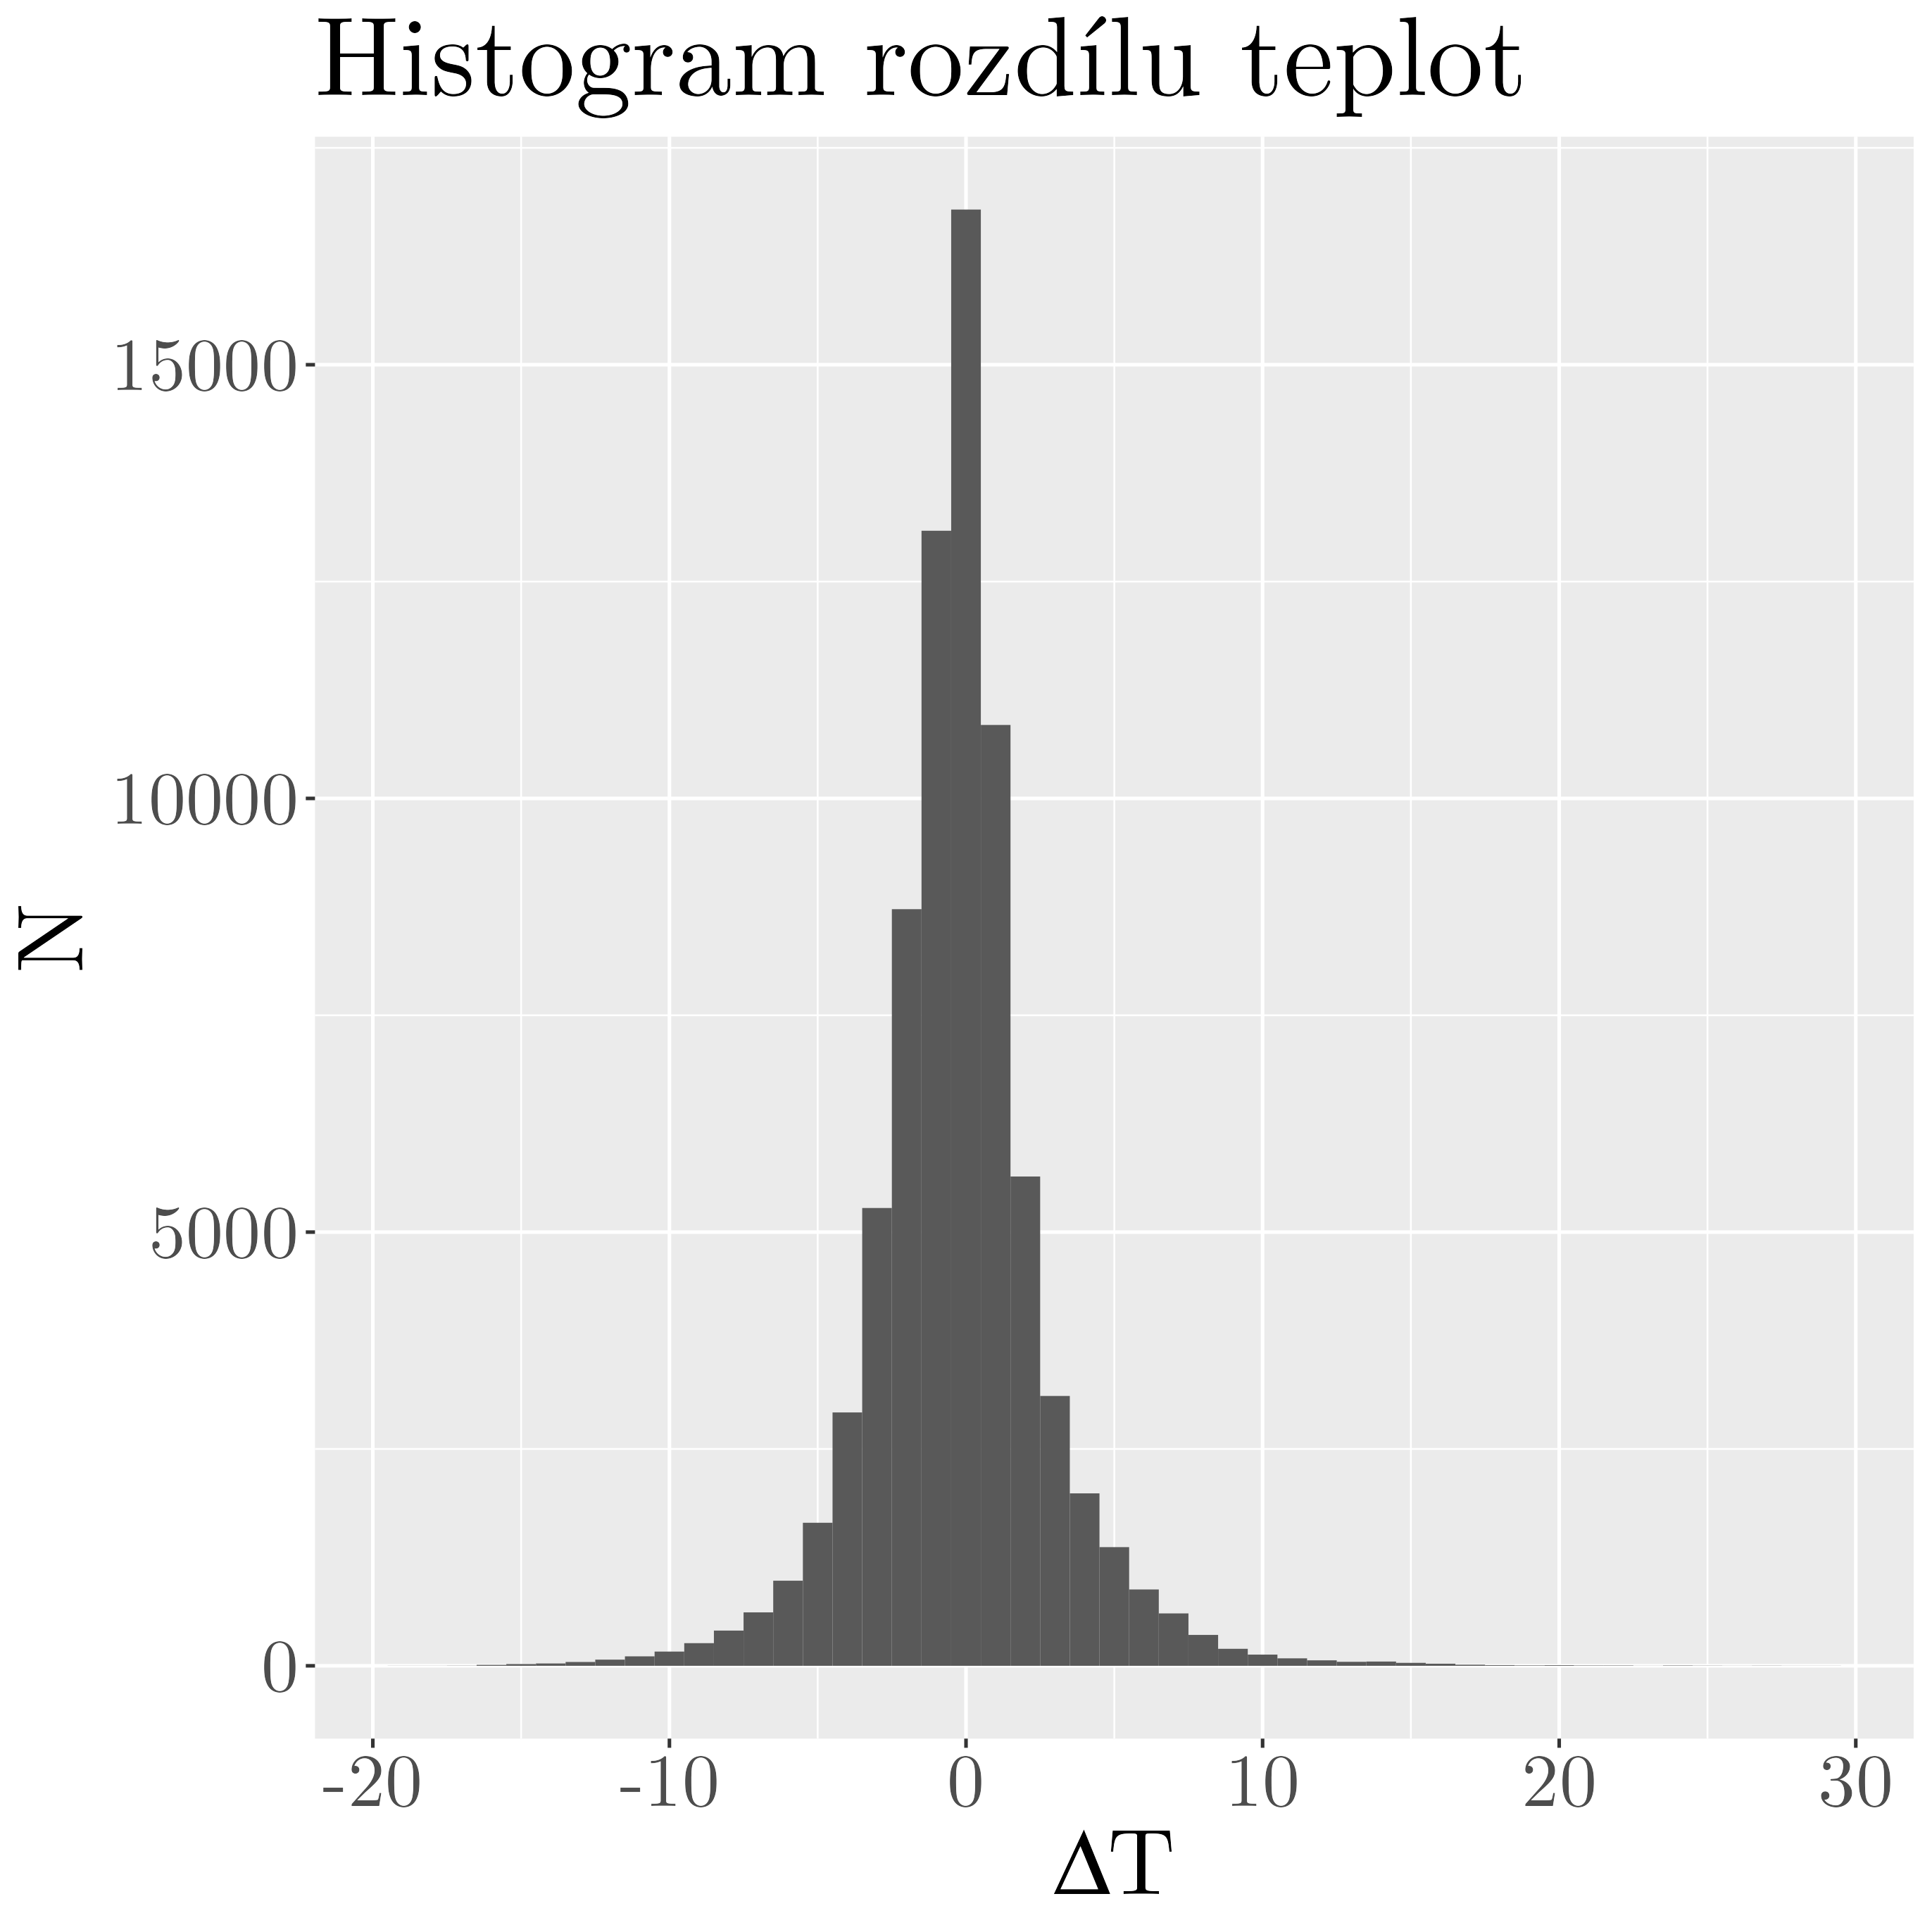
\includegraphics[width=\textwidth]{img/ch2/hist_diff_max0cm.png}
		\caption{Histogram rozdílu maximálních teplot v $\SI{0}{cm}$ a $\SI{2}{m}$. $\text{M} = -0.24$, $\text{MD} = -0.25$.}
		\label{fig:hist_diff_max0cm}
	\end{subfigure}
	\hfill
	\begin{subfigure}{0.45\textwidth}
  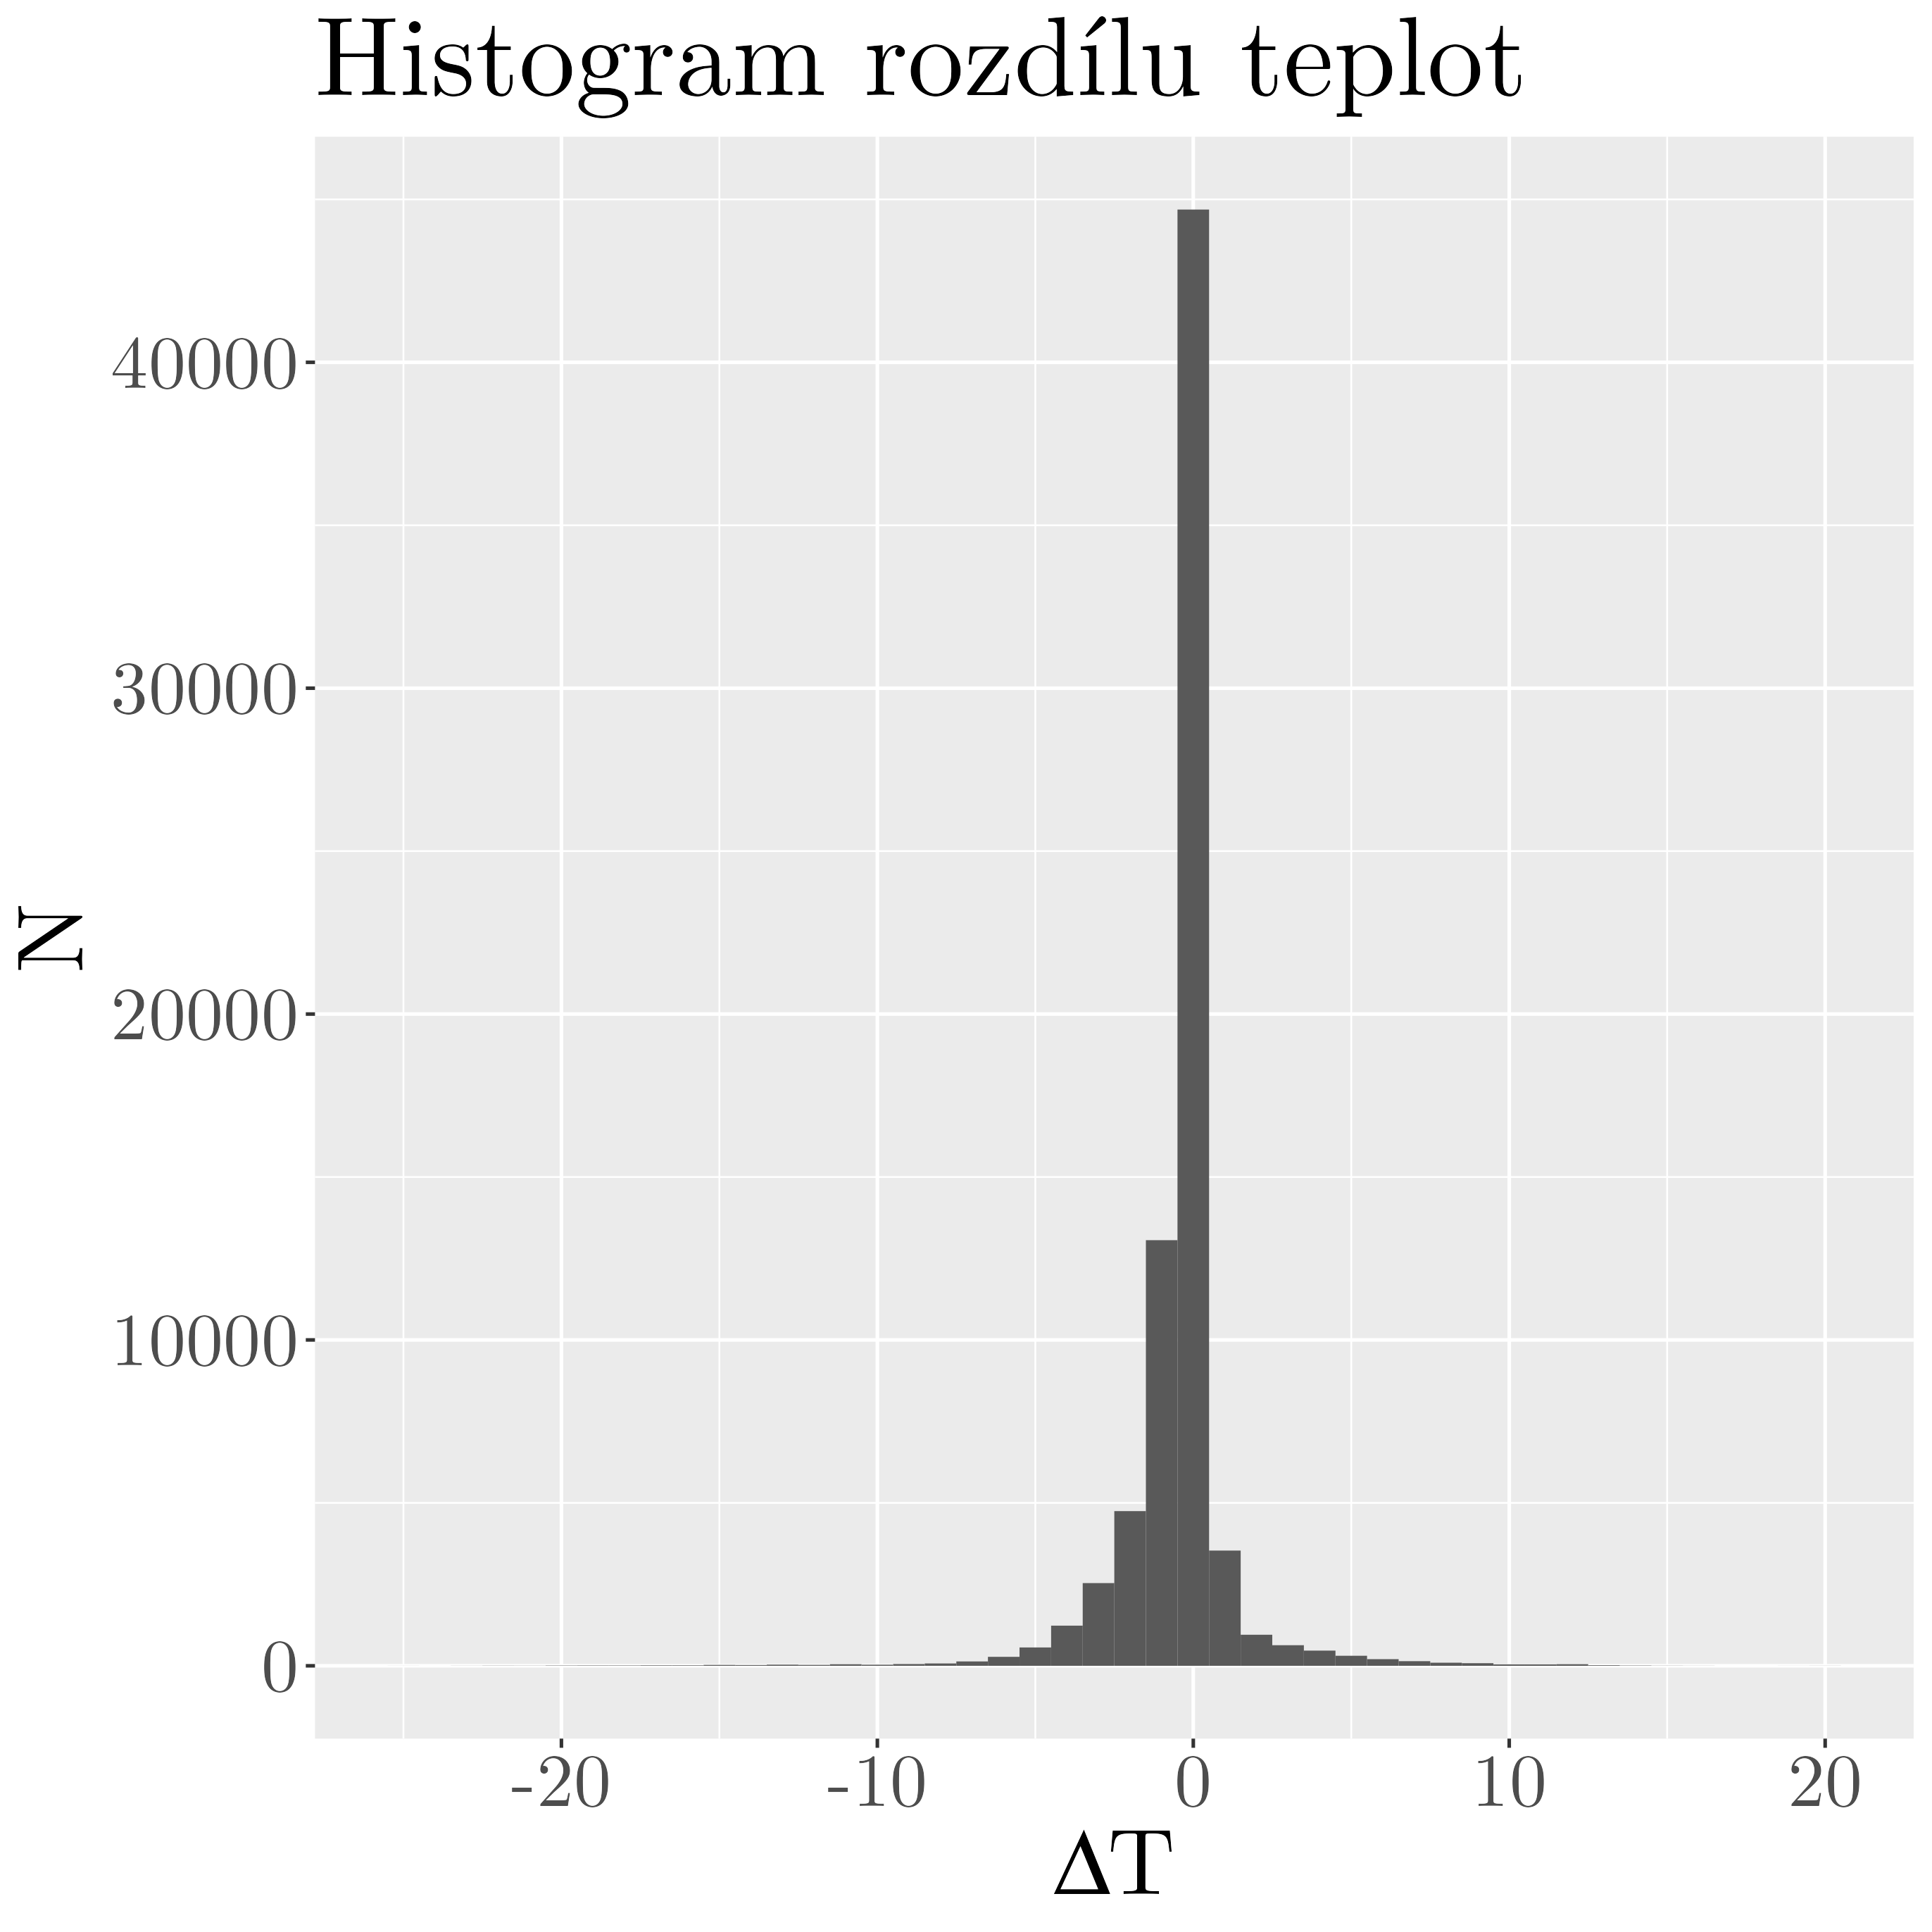
\includegraphics[width=\textwidth]{img/ch2/hist_diff_min15cm.png}
		\caption{Histogram rozdílu minimálních teplot v $\SI{15}{cm}$ a $\SI{2}{m}$. $\text{M} = -0.36$, $\text{MD} = -0.125$.}
		\label{fig:hist_diff_min15cm}
	\end{subfigure}
	\hfill
	\begin{subfigure}{0.45\textwidth}
  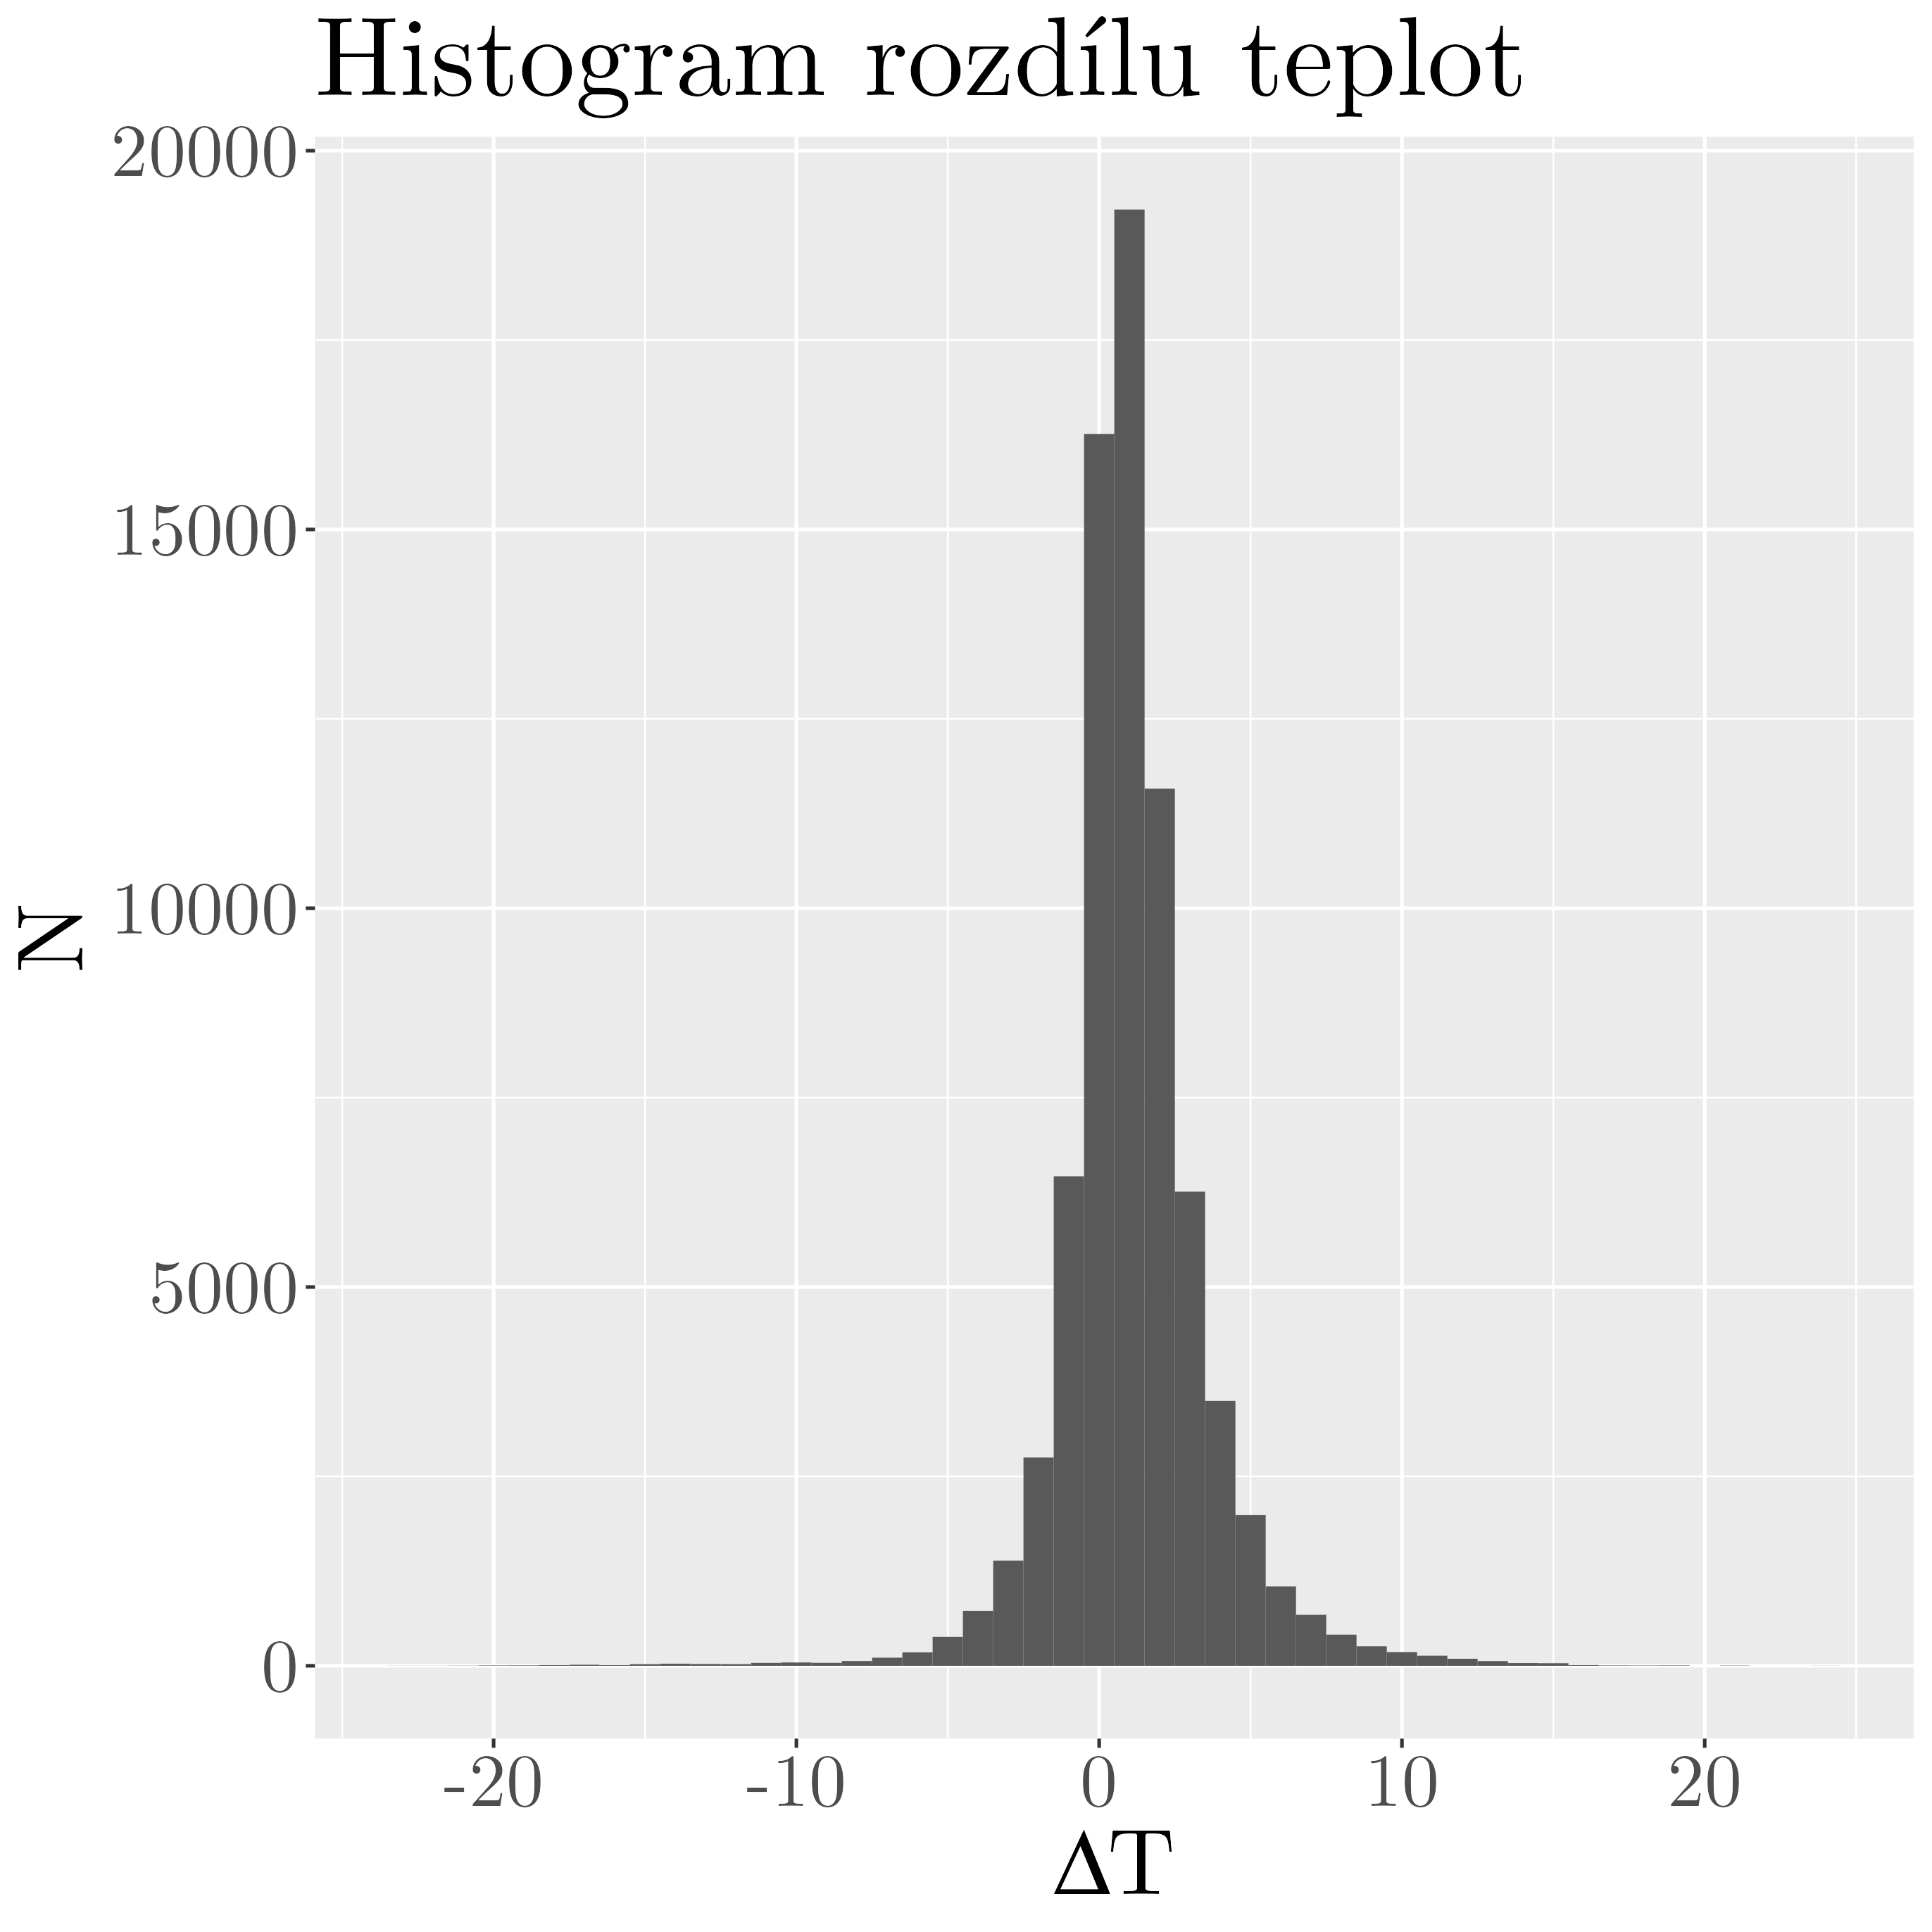
\includegraphics[width=\textwidth]{img/ch2/hist_diff_min0cm.png}
		\caption{Histogram rozdílu miniálních teplot v $\SI{0}{cm}$ a $\SI{2}{m}$. $\text{M} = 1.14$, $\text{MD} = 0.9375$.}
		\label{fig:hist_diff_min0cm}
	\end{subfigure}
	\caption{Histogramy rozdílů maximální resp. minimální teploty v $\SI{15}{cm}$ resp. v $\SI{0}{cm}$ a ve $\SI{2}{m}$. K tomu odpovídající hodnoty, průměru $\text{M}$ a mediánu $\text{MD}$.}
	\label{fig:hist_diff}
\end{figure}


\section{Metody analýzy dat}\label{chap:methods}
Cílem následující části je ukázat jakým způsobem byla data zpracována, proč byl vybrán daný model a ukázat ověření metody ověření předpokladů.

\subsection{Korelace dat}
Z povahy naměřených dat je zřejmé, že zde bude existovat autokorelace mezi naměřenými maximálními nebo minimálními teplotami. Autokorelace se pak projeví i u rozdílu teploty naměřené blízko země a ve $\SI{2}{m}$. Na obrázku \ref{fig:acf} vidíme autokorelační funkci pro jedno z čidel.

\begin{figure}
	\centering
	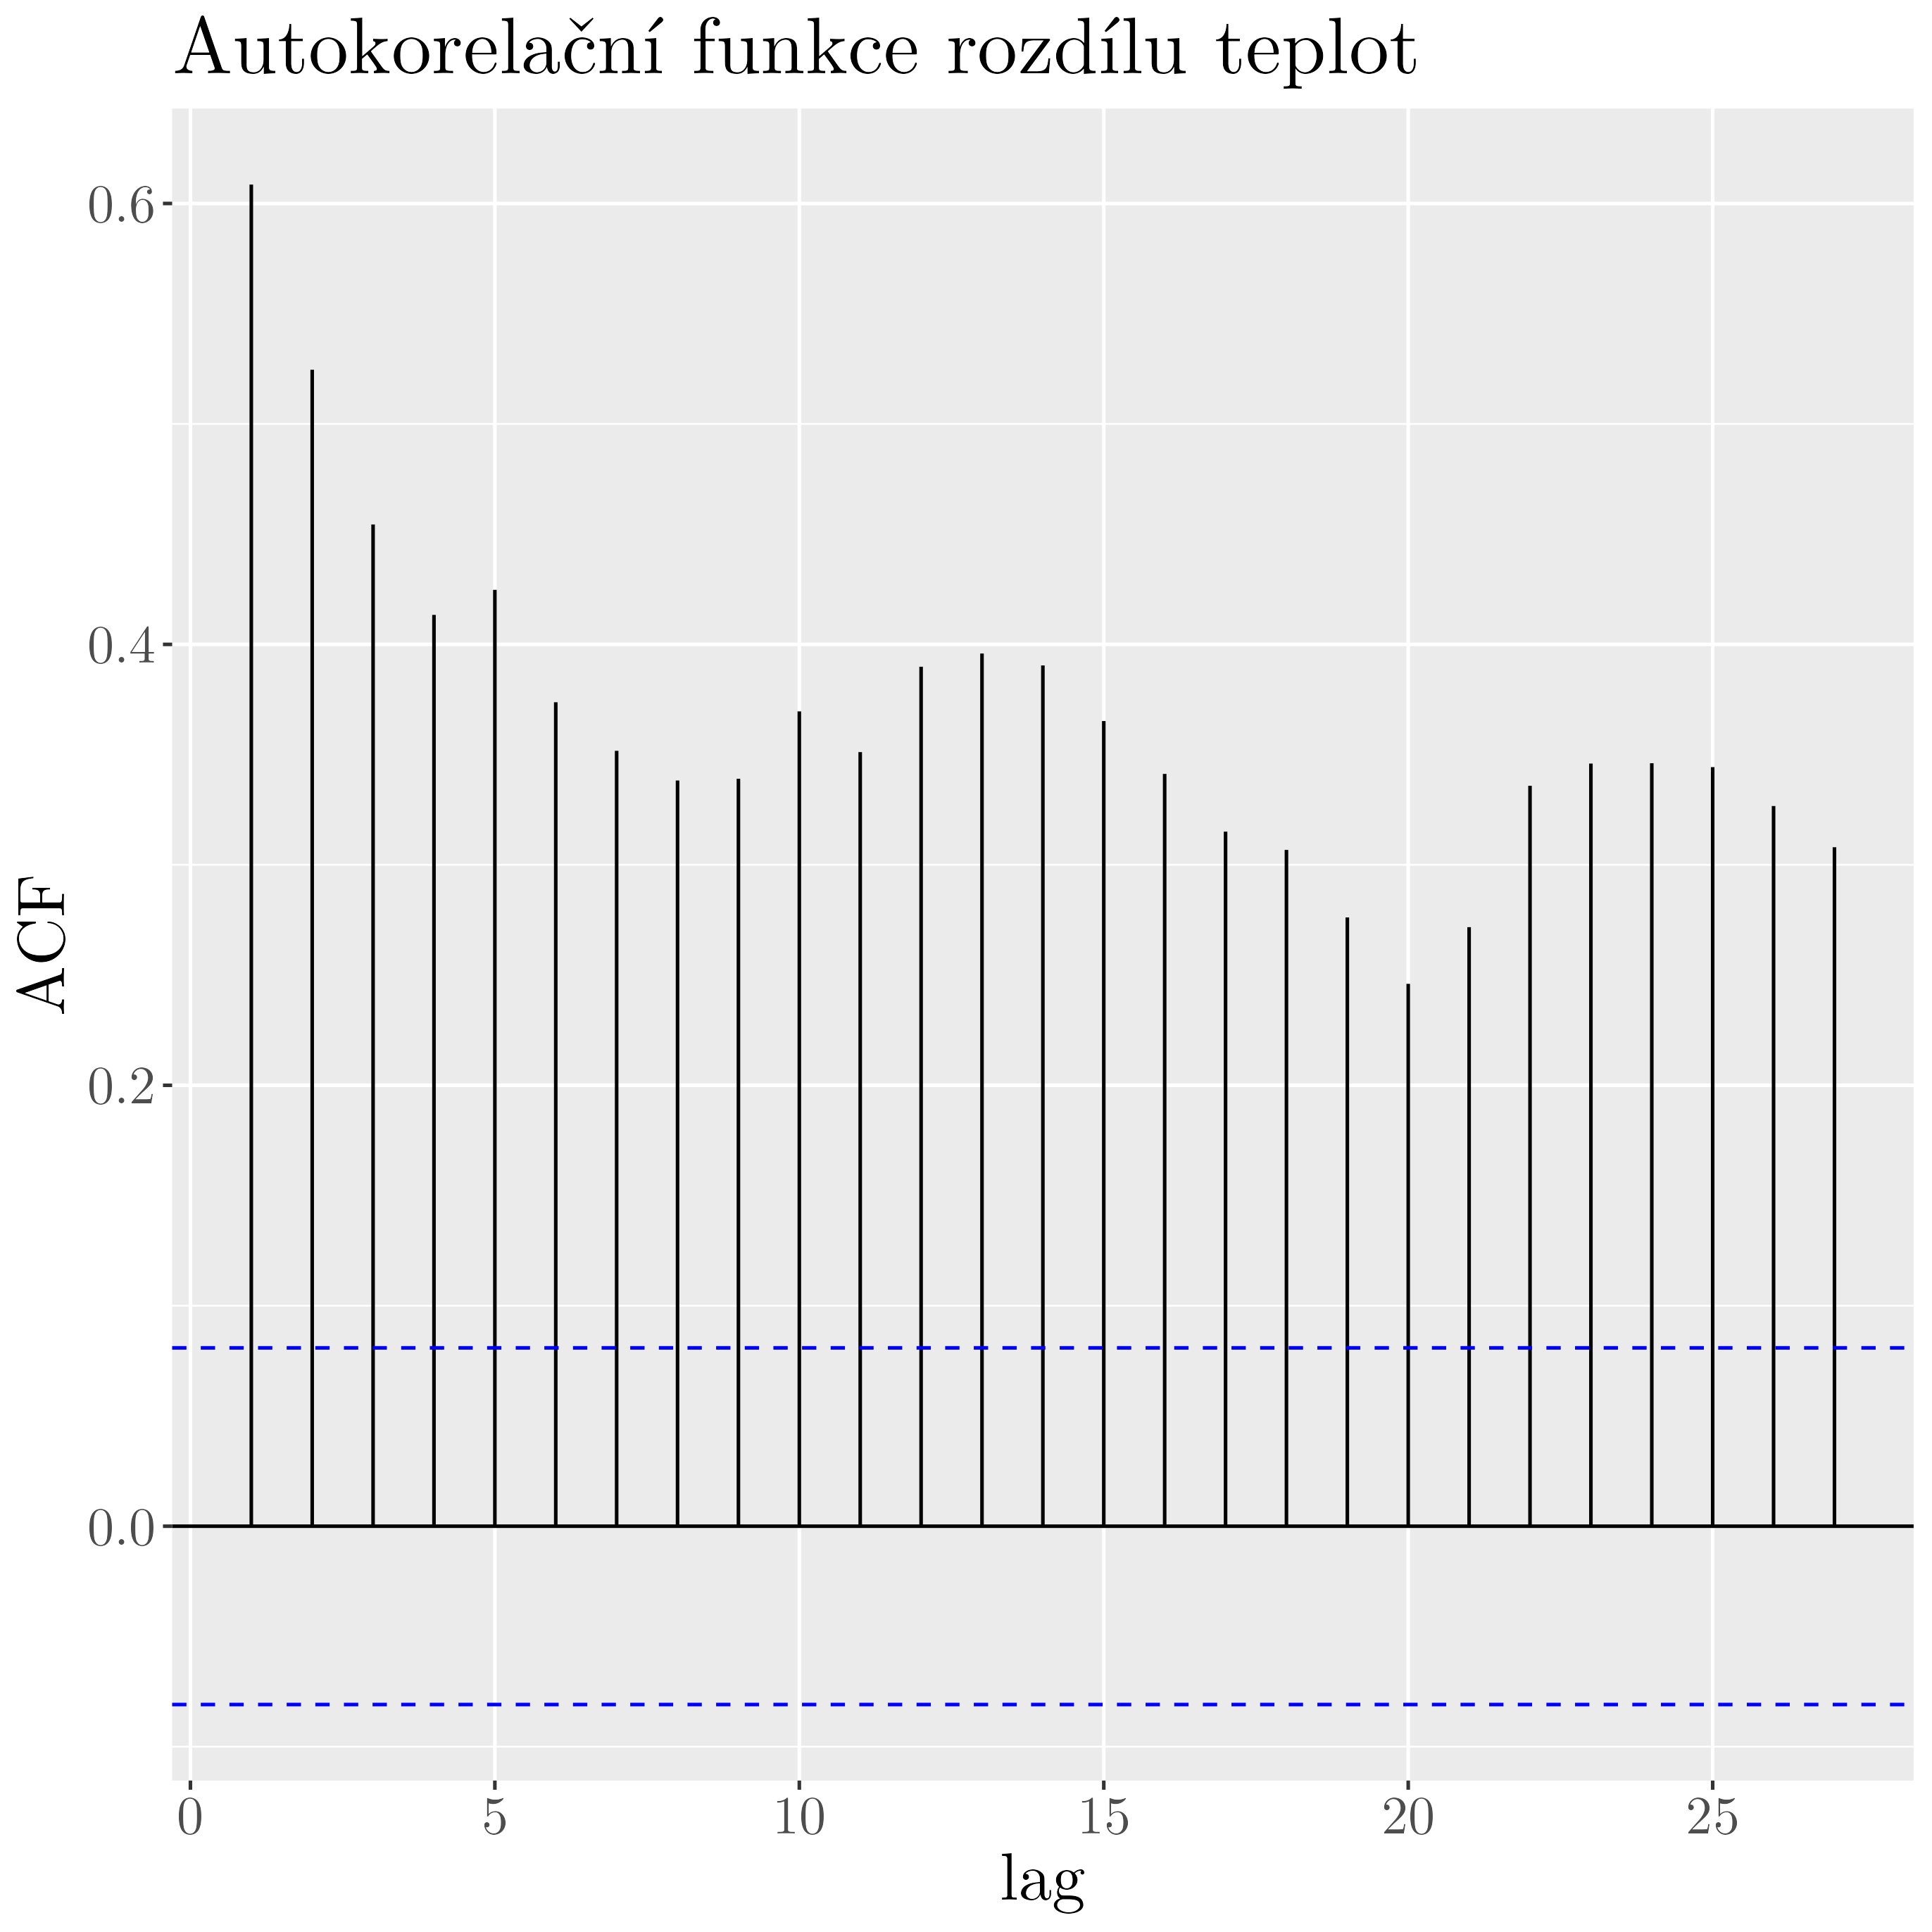
\includegraphics[width=0.55\textwidth]{img/ch2/acfNPS_4311_D_TMS.png}
	\caption{Autokorelační funkce pro rozdíl teplot mezi maximální teplotou v $\SI{15}{cm}$ a teplotou ve $\SI{2}{m}$ na páru čidel nejblíže meteorologické stanici Churáňov.}
	\label{fig:acf}
\end{figure}

Autokorelace není takto významná pro všechna čidla, ale i tak nám vylučuje možnost využít jednoduché mnohonásobné lineární regrese.

Vzhledem k tomu, že pracujeme s daty rozloženými v prostoru, otestujeme jestli mezi nimi existuje prostorová korelace. Využijeme teorii popsanou v odstavci \ref{chap:variogram}. Na obrázcích \ref{fig:variograms} vidíme dvanáct semivariogramů pro každý první den měsíce v roce 2020. Kvůli lišícím se hodnotám semivariance nemůžeme semivariogramy zakreslit do jednoho grafu. Ze semivariogramů můžeme usoudit, že v datech neexistuje významná prostorová korelace, kterou bychom museli v modelu zohlednit.

\begin{figure}
	\centering
	\begin{subfigure}{0.30\textwidth}
		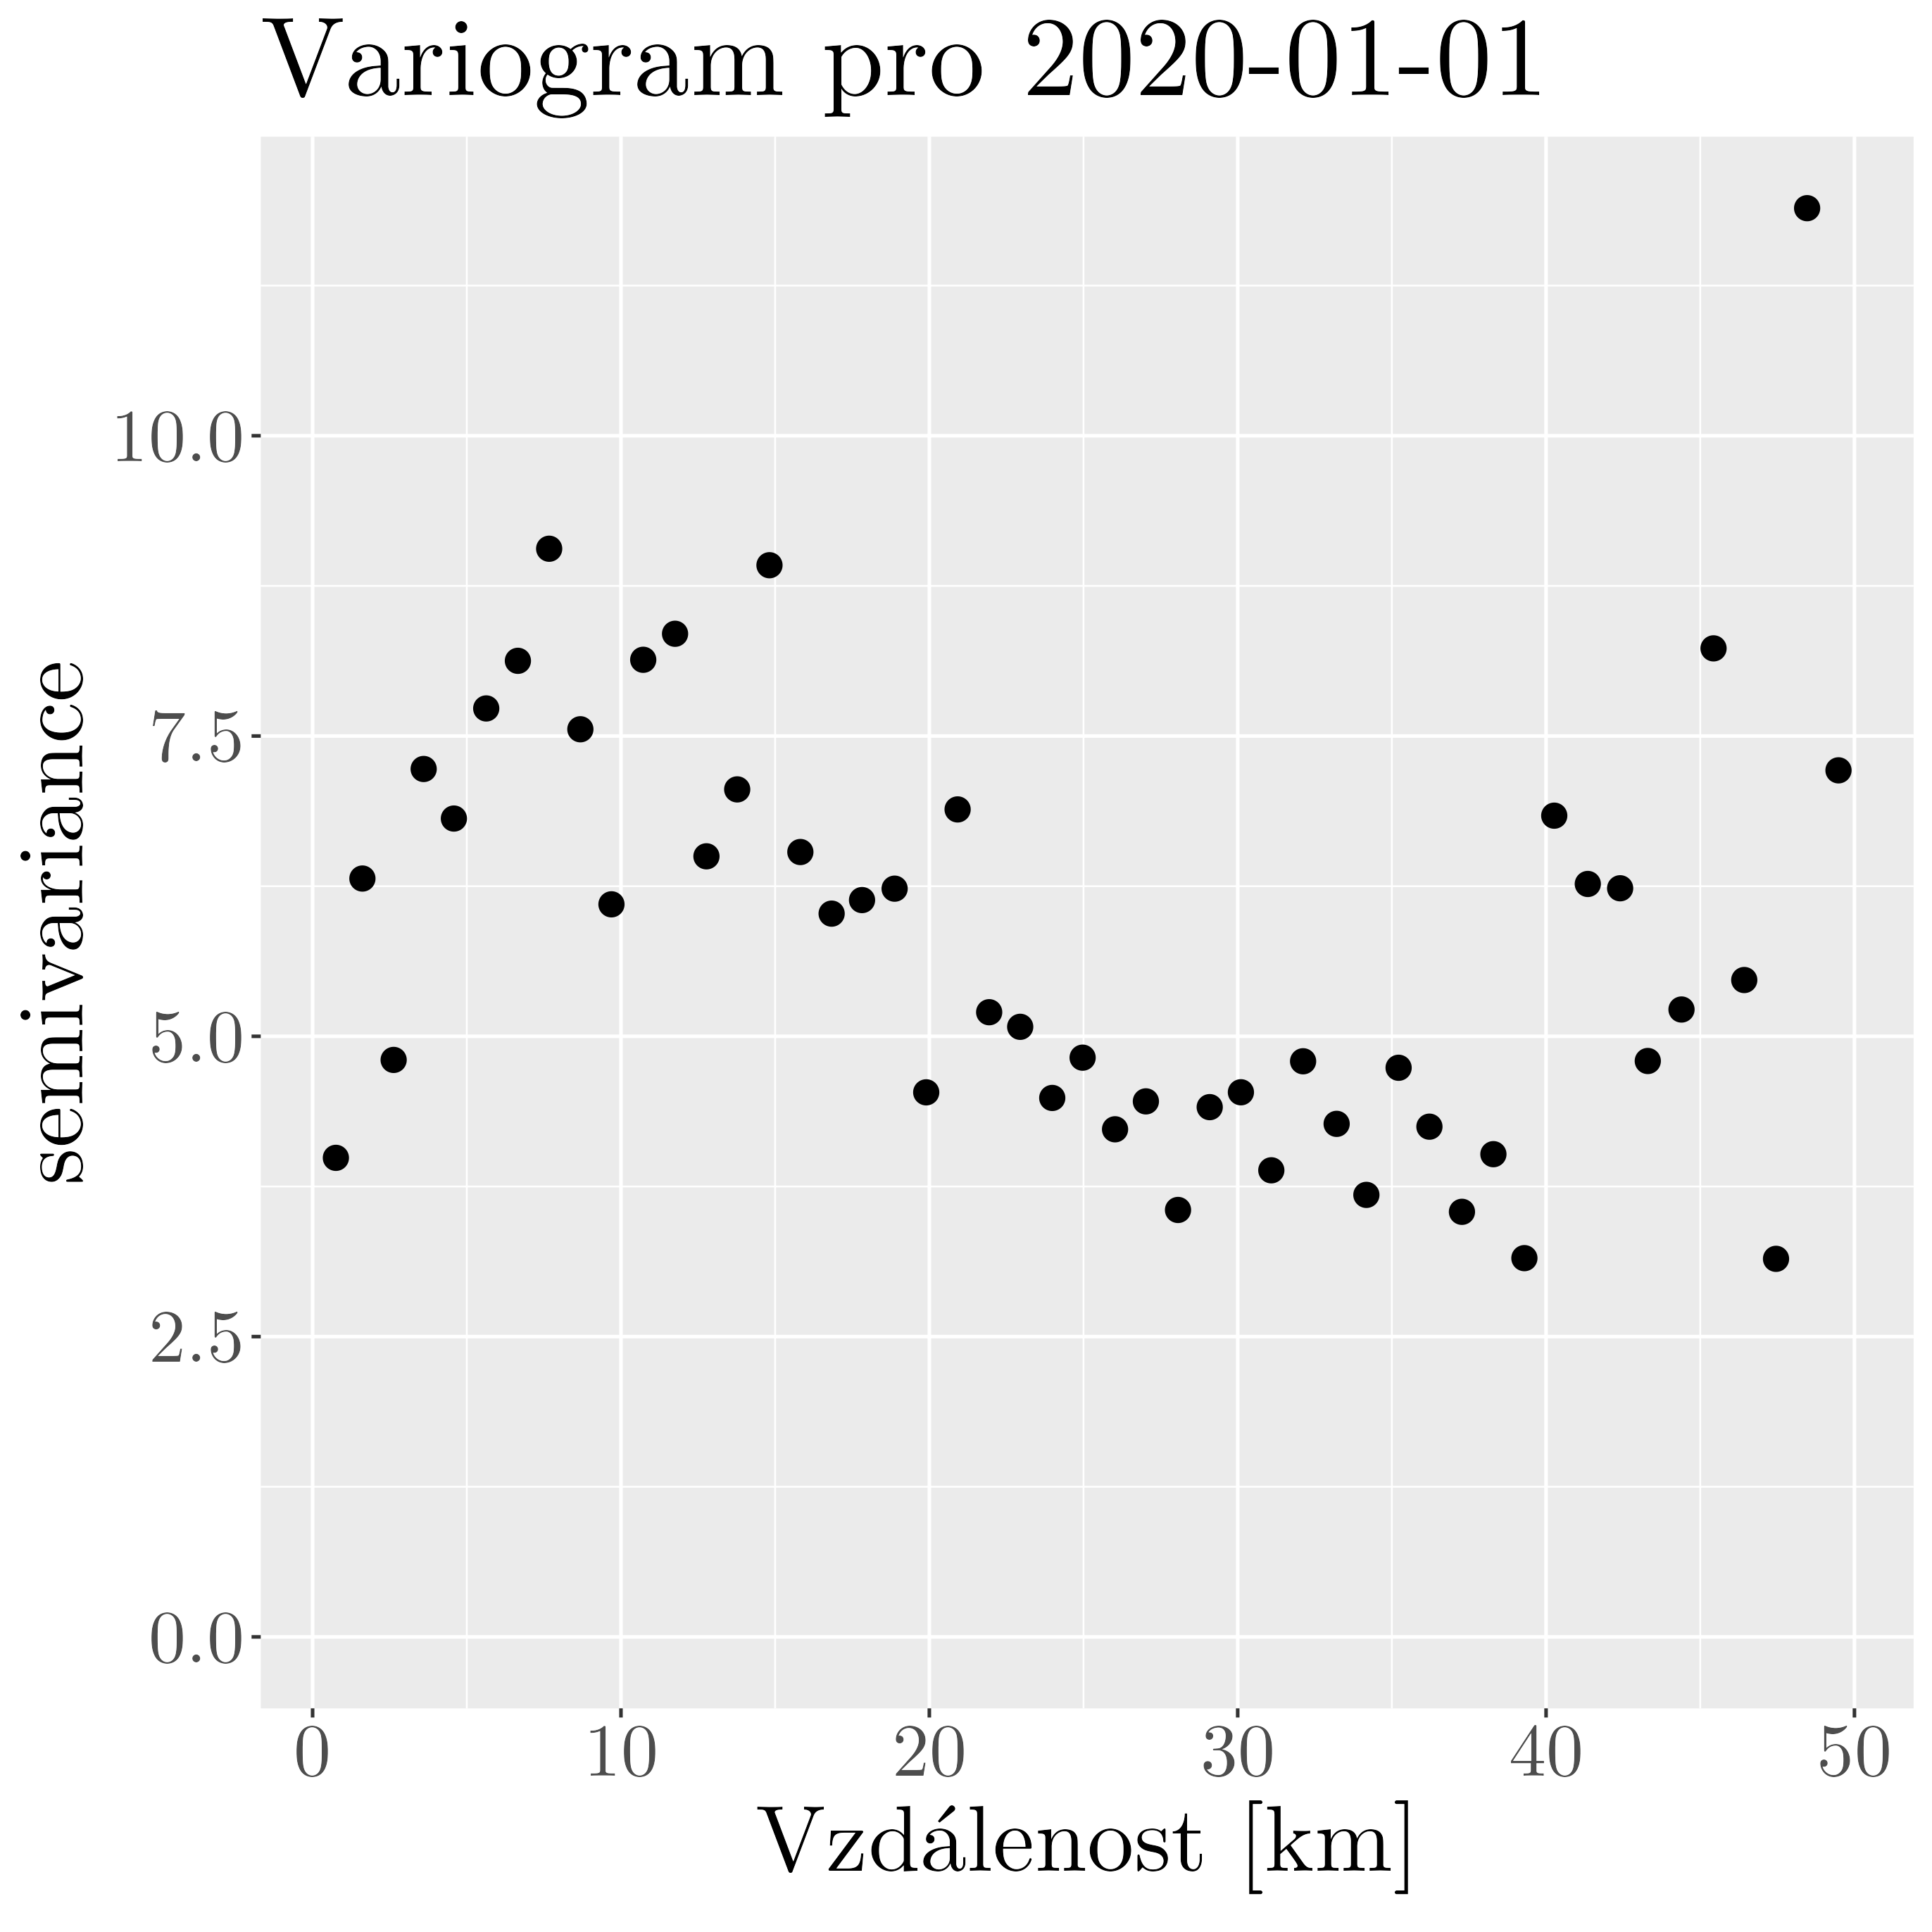
\includegraphics[width=\textwidth]{img/ch2/variograms/variogram_max15cm1.png}
		\caption{}
		\label{fig:variogram1}
	\end{subfigure}
	\hfill
	\begin{subfigure}{0.30\textwidth}
		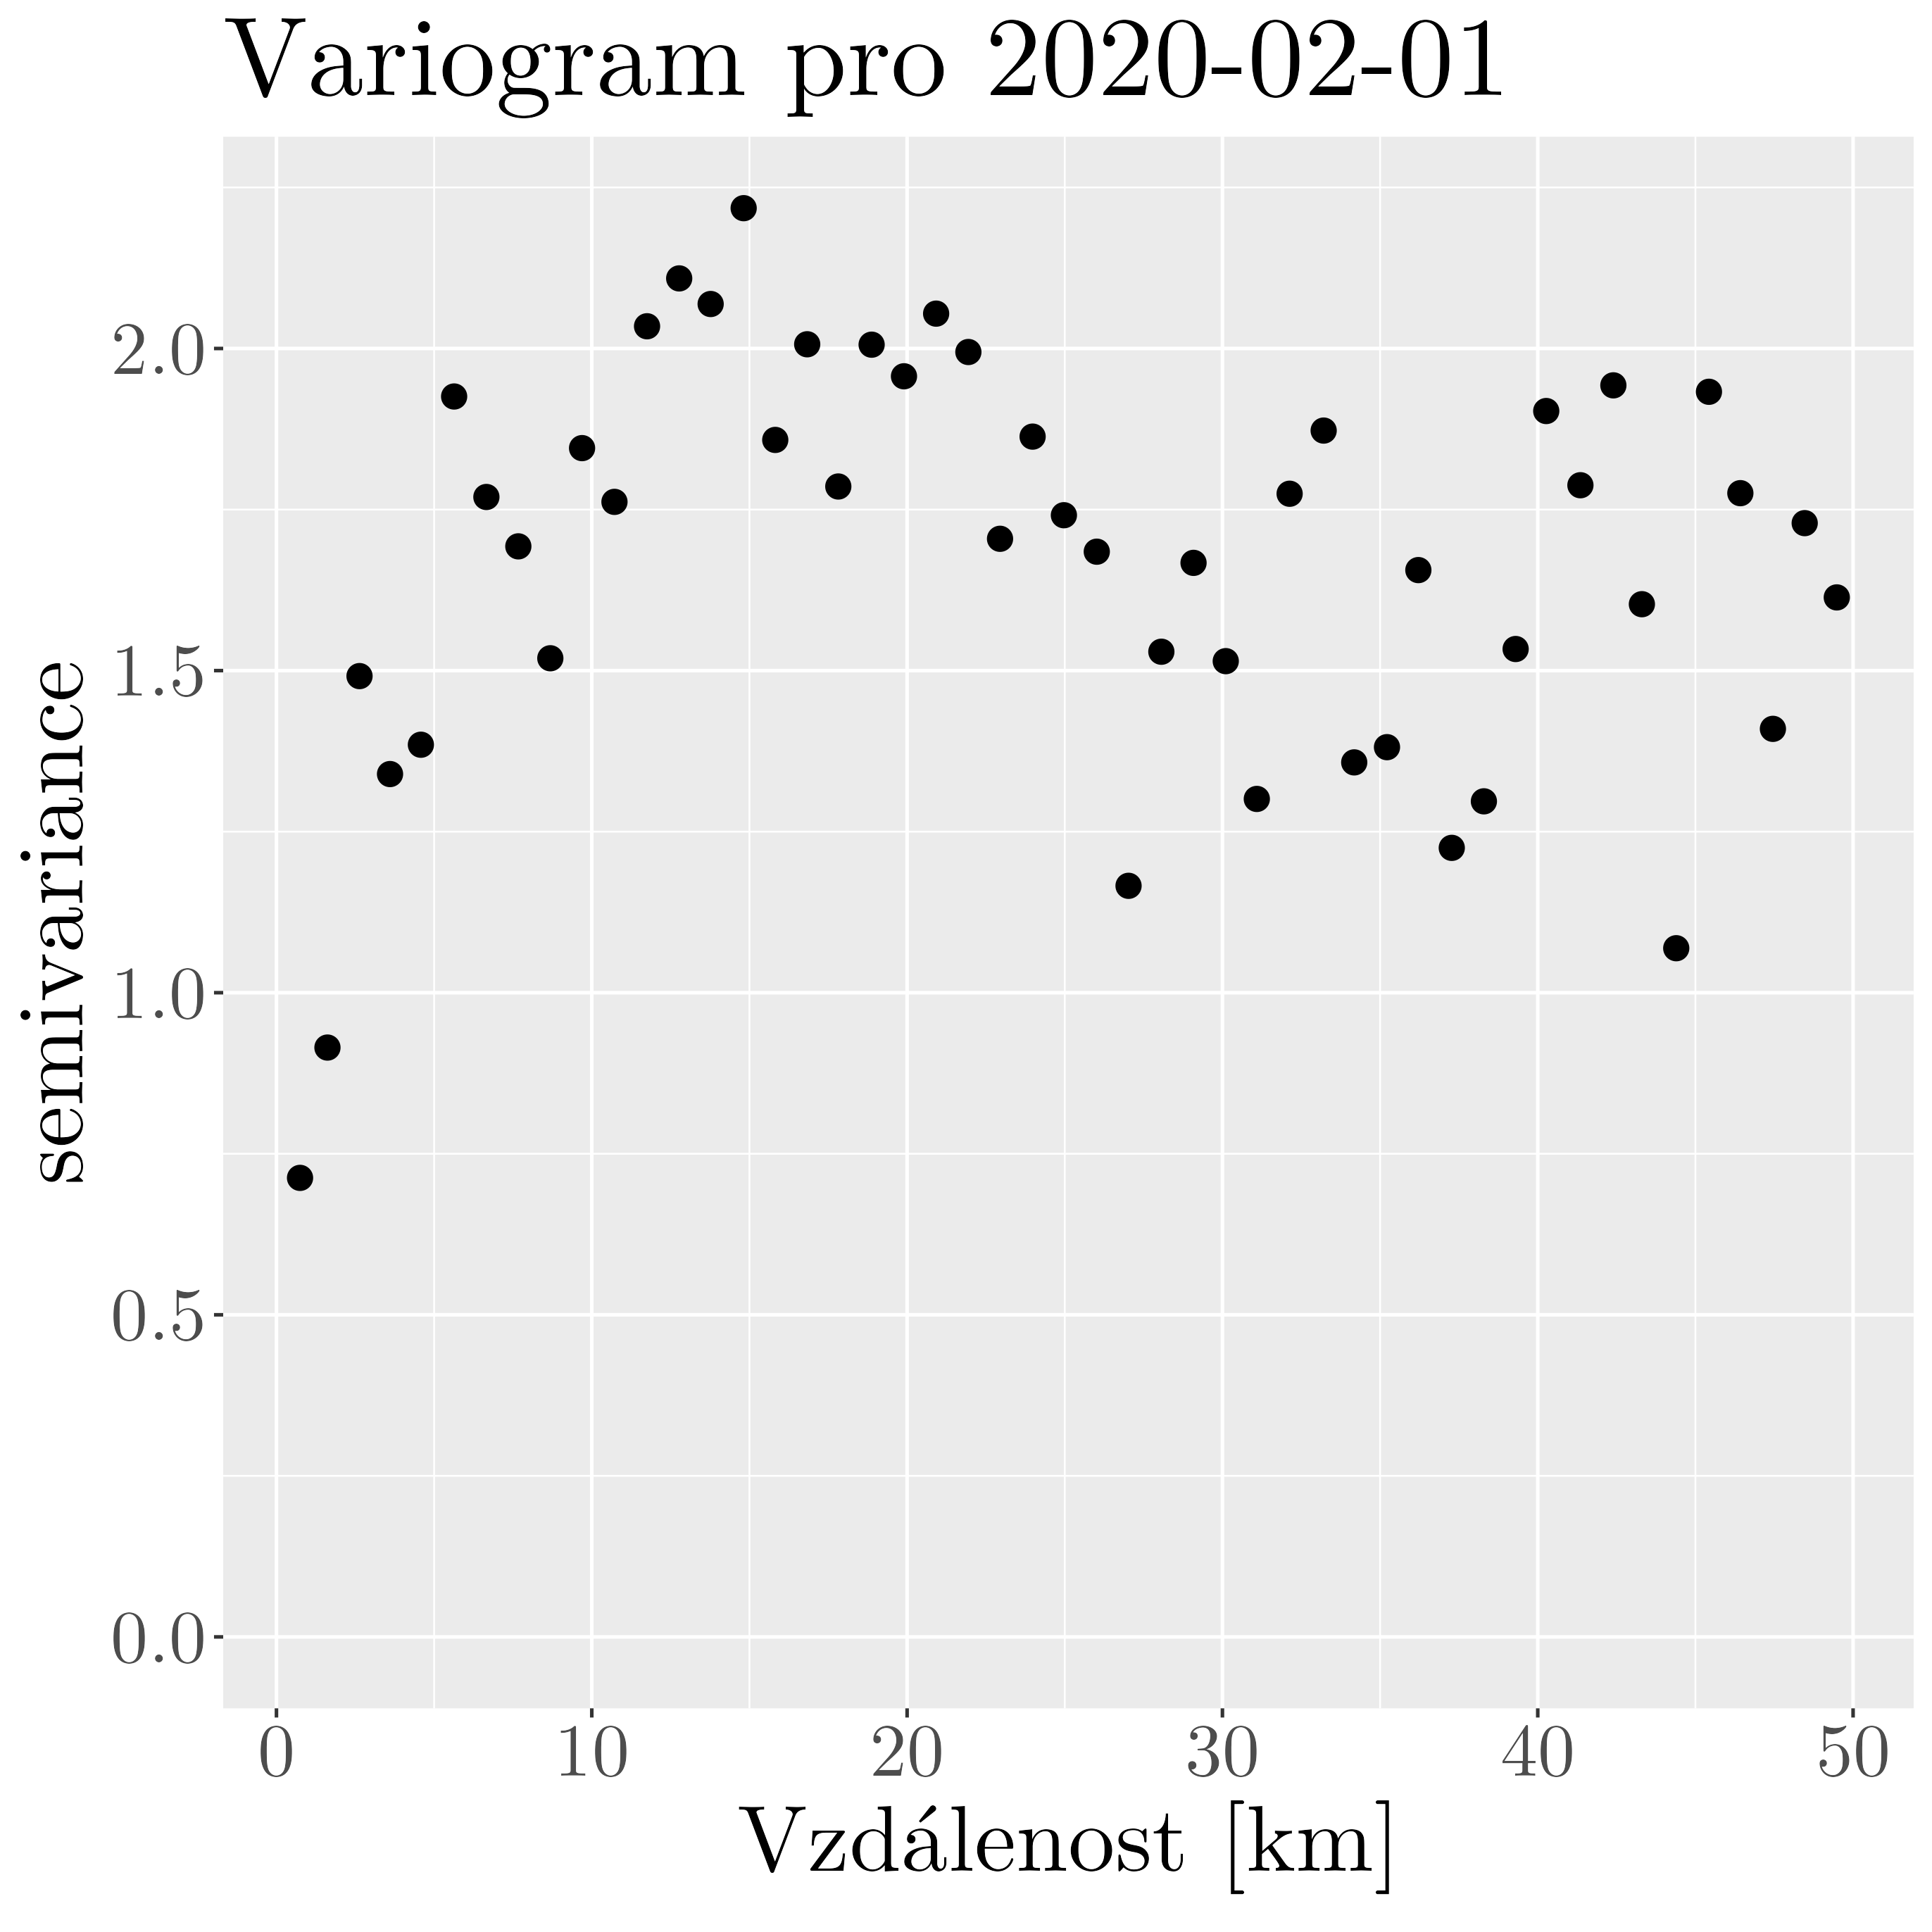
\includegraphics[width=\textwidth]{img/ch2/variograms/variogram_max15cm2.png}
		\caption{}
		\label{fig:variogram2}
	\end{subfigure}
	\hfill
	\begin{subfigure}{0.30\textwidth}
		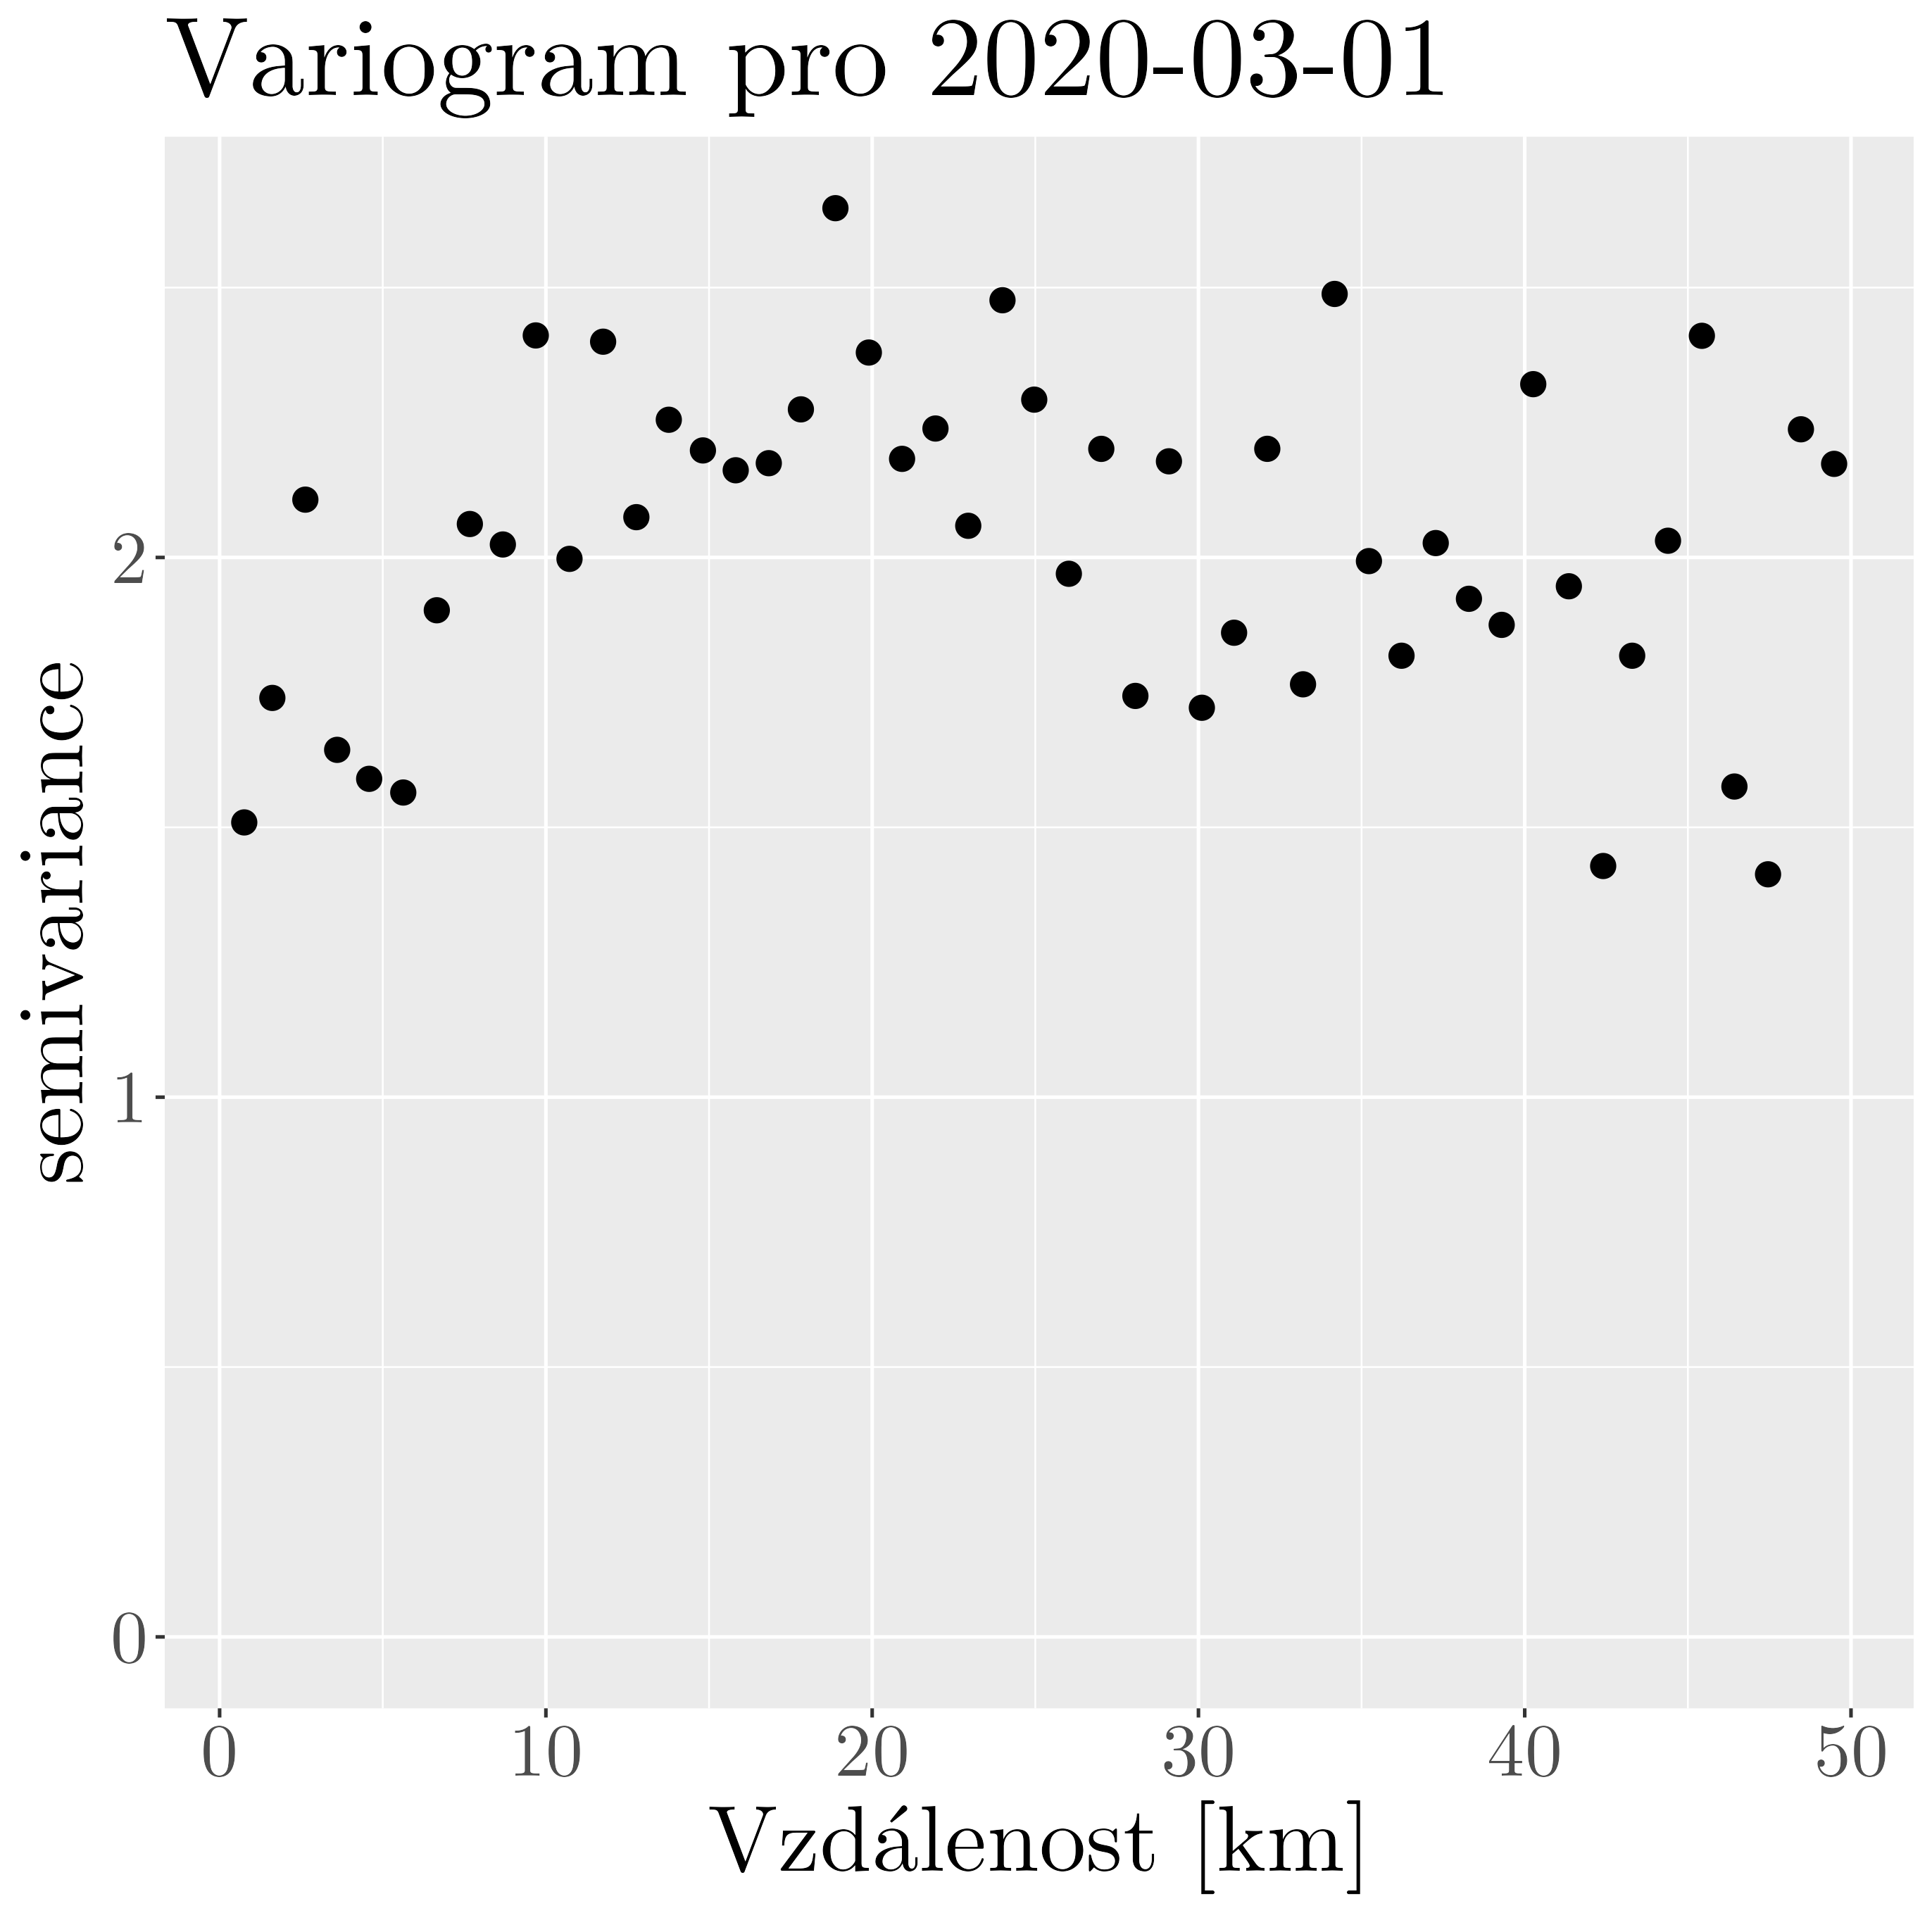
\includegraphics[width=\textwidth]{img/ch2/variograms/variogram_max15cm3.png}
		\caption{}
		\label{fig:variogram3}
	\end{subfigure}
	\hfill
	\begin{subfigure}{0.30\textwidth}
		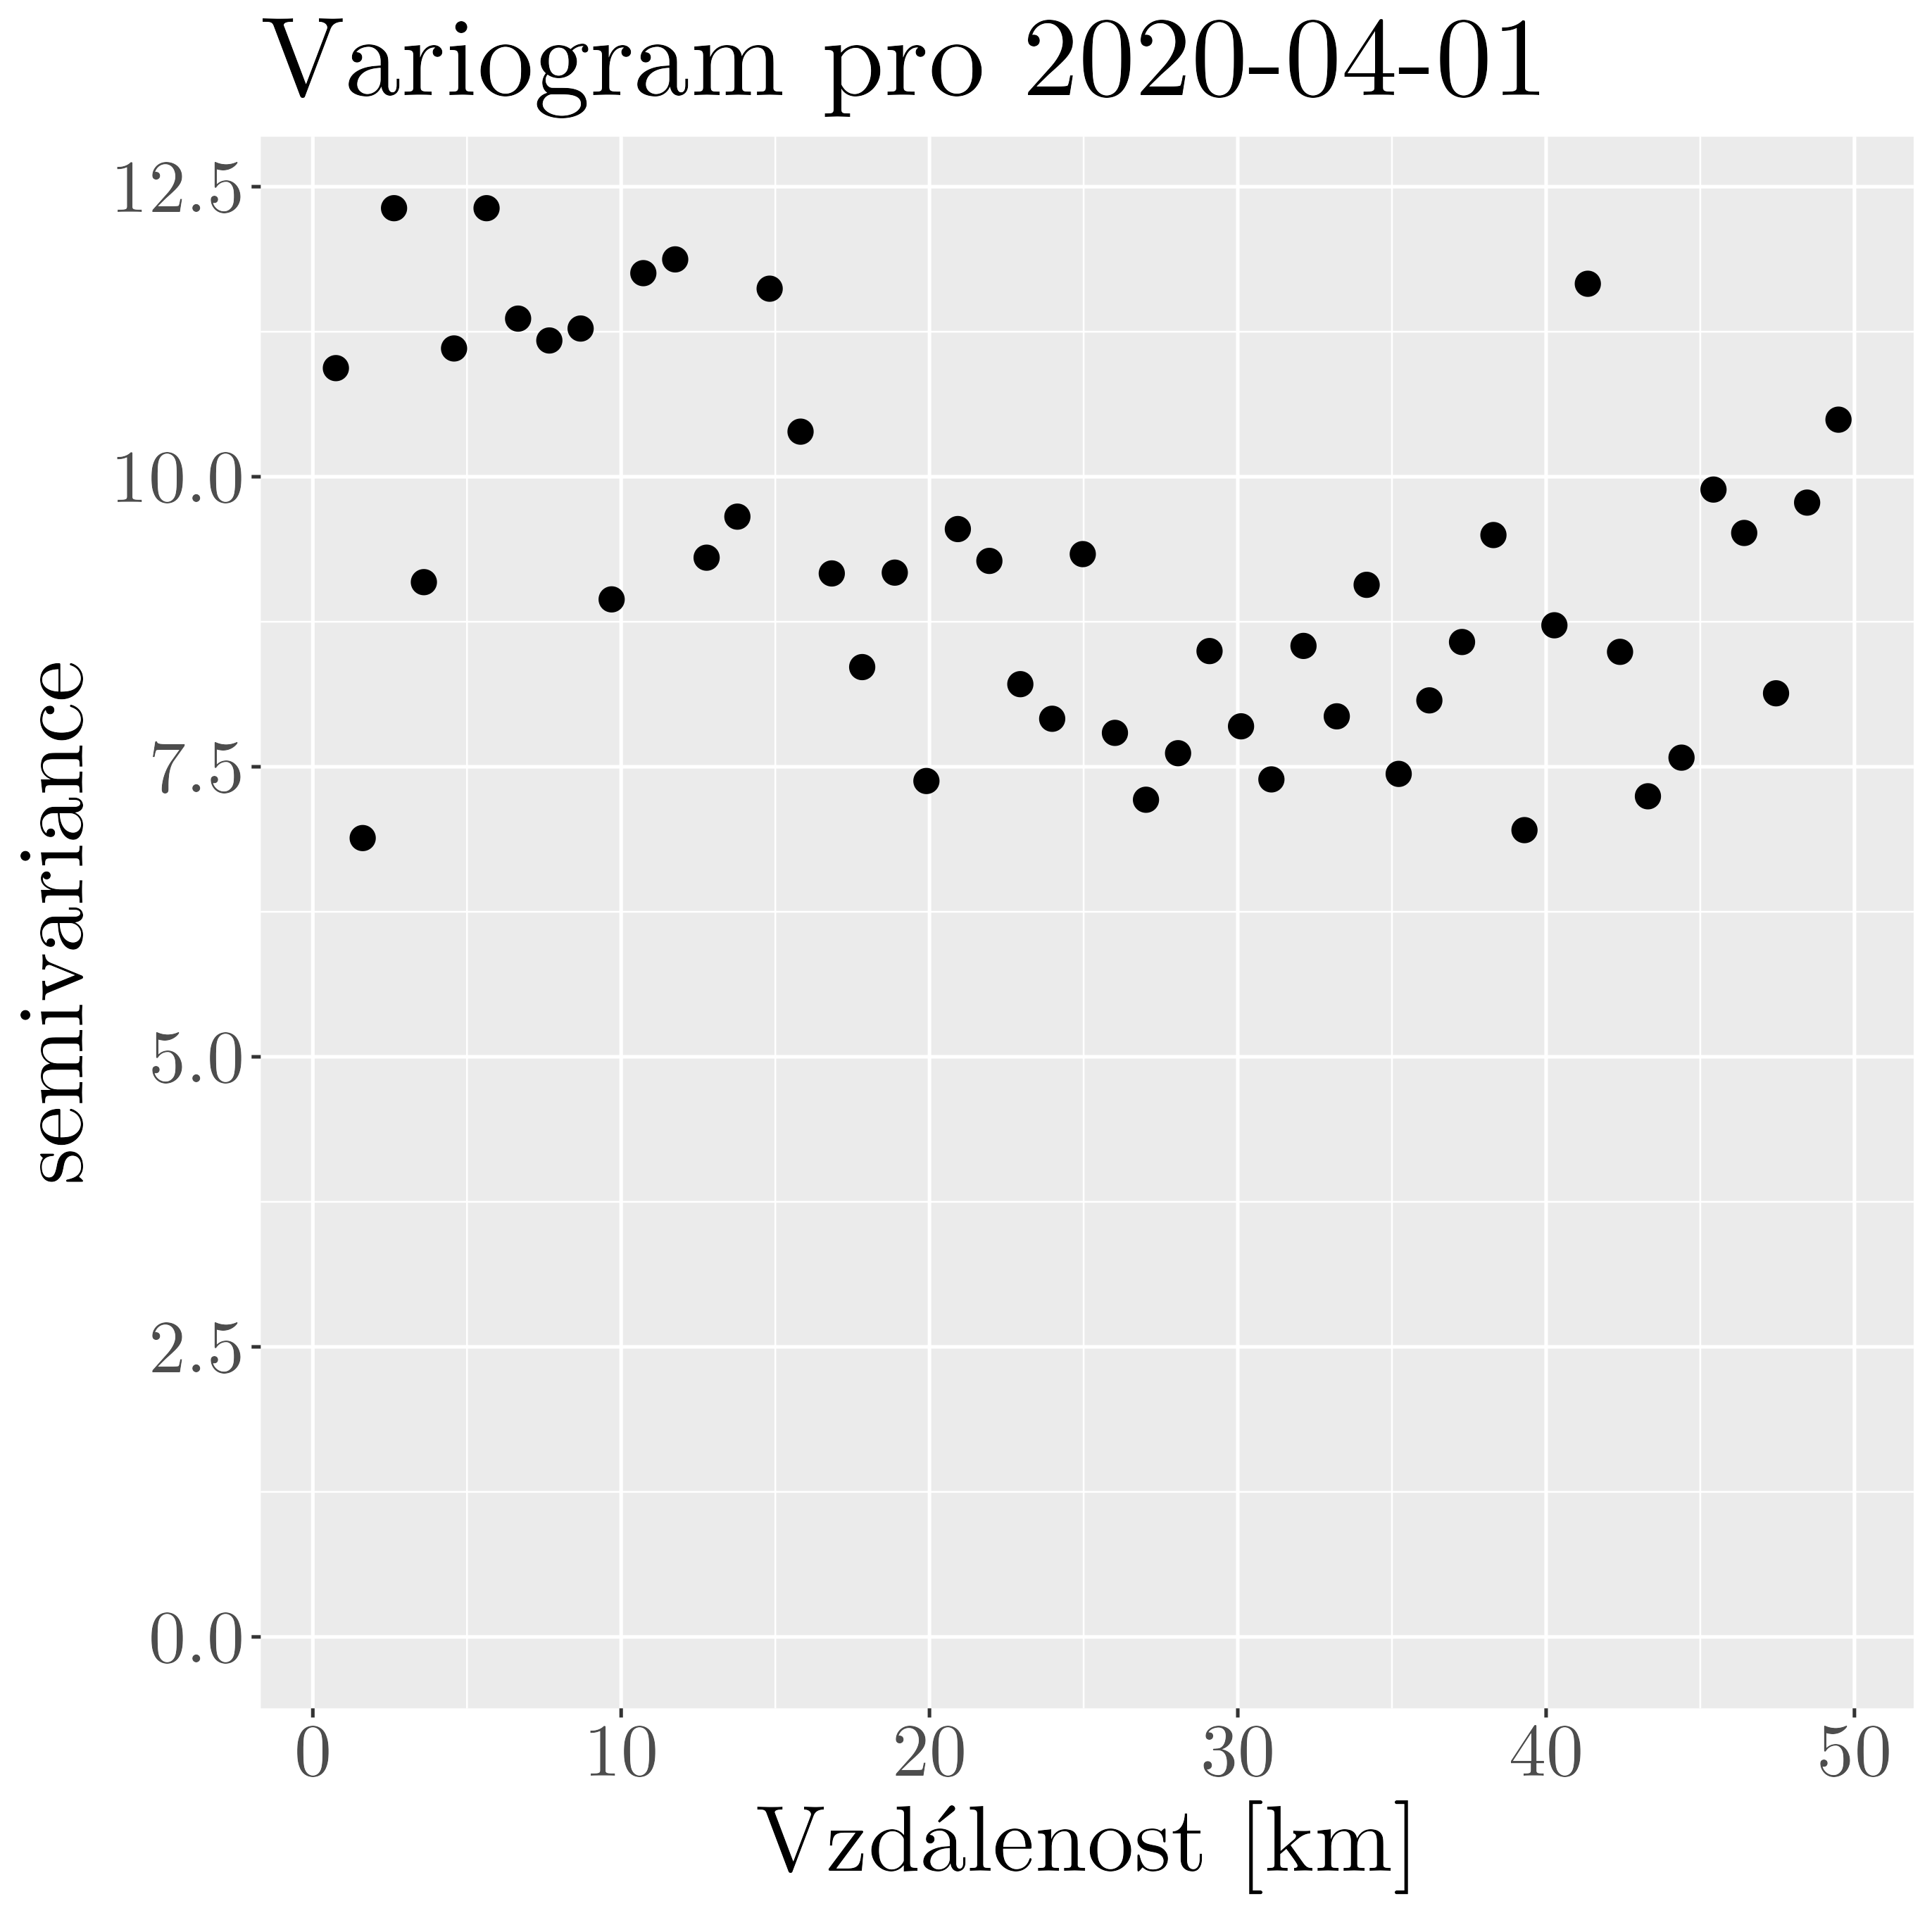
\includegraphics[width=\textwidth]{img/ch2/variograms/variogram_max15cm4.png}
		\caption{}
		\label{fig:variogram4}
	\end{subfigure}
	\hfill
	\begin{subfigure}{0.30\textwidth}
		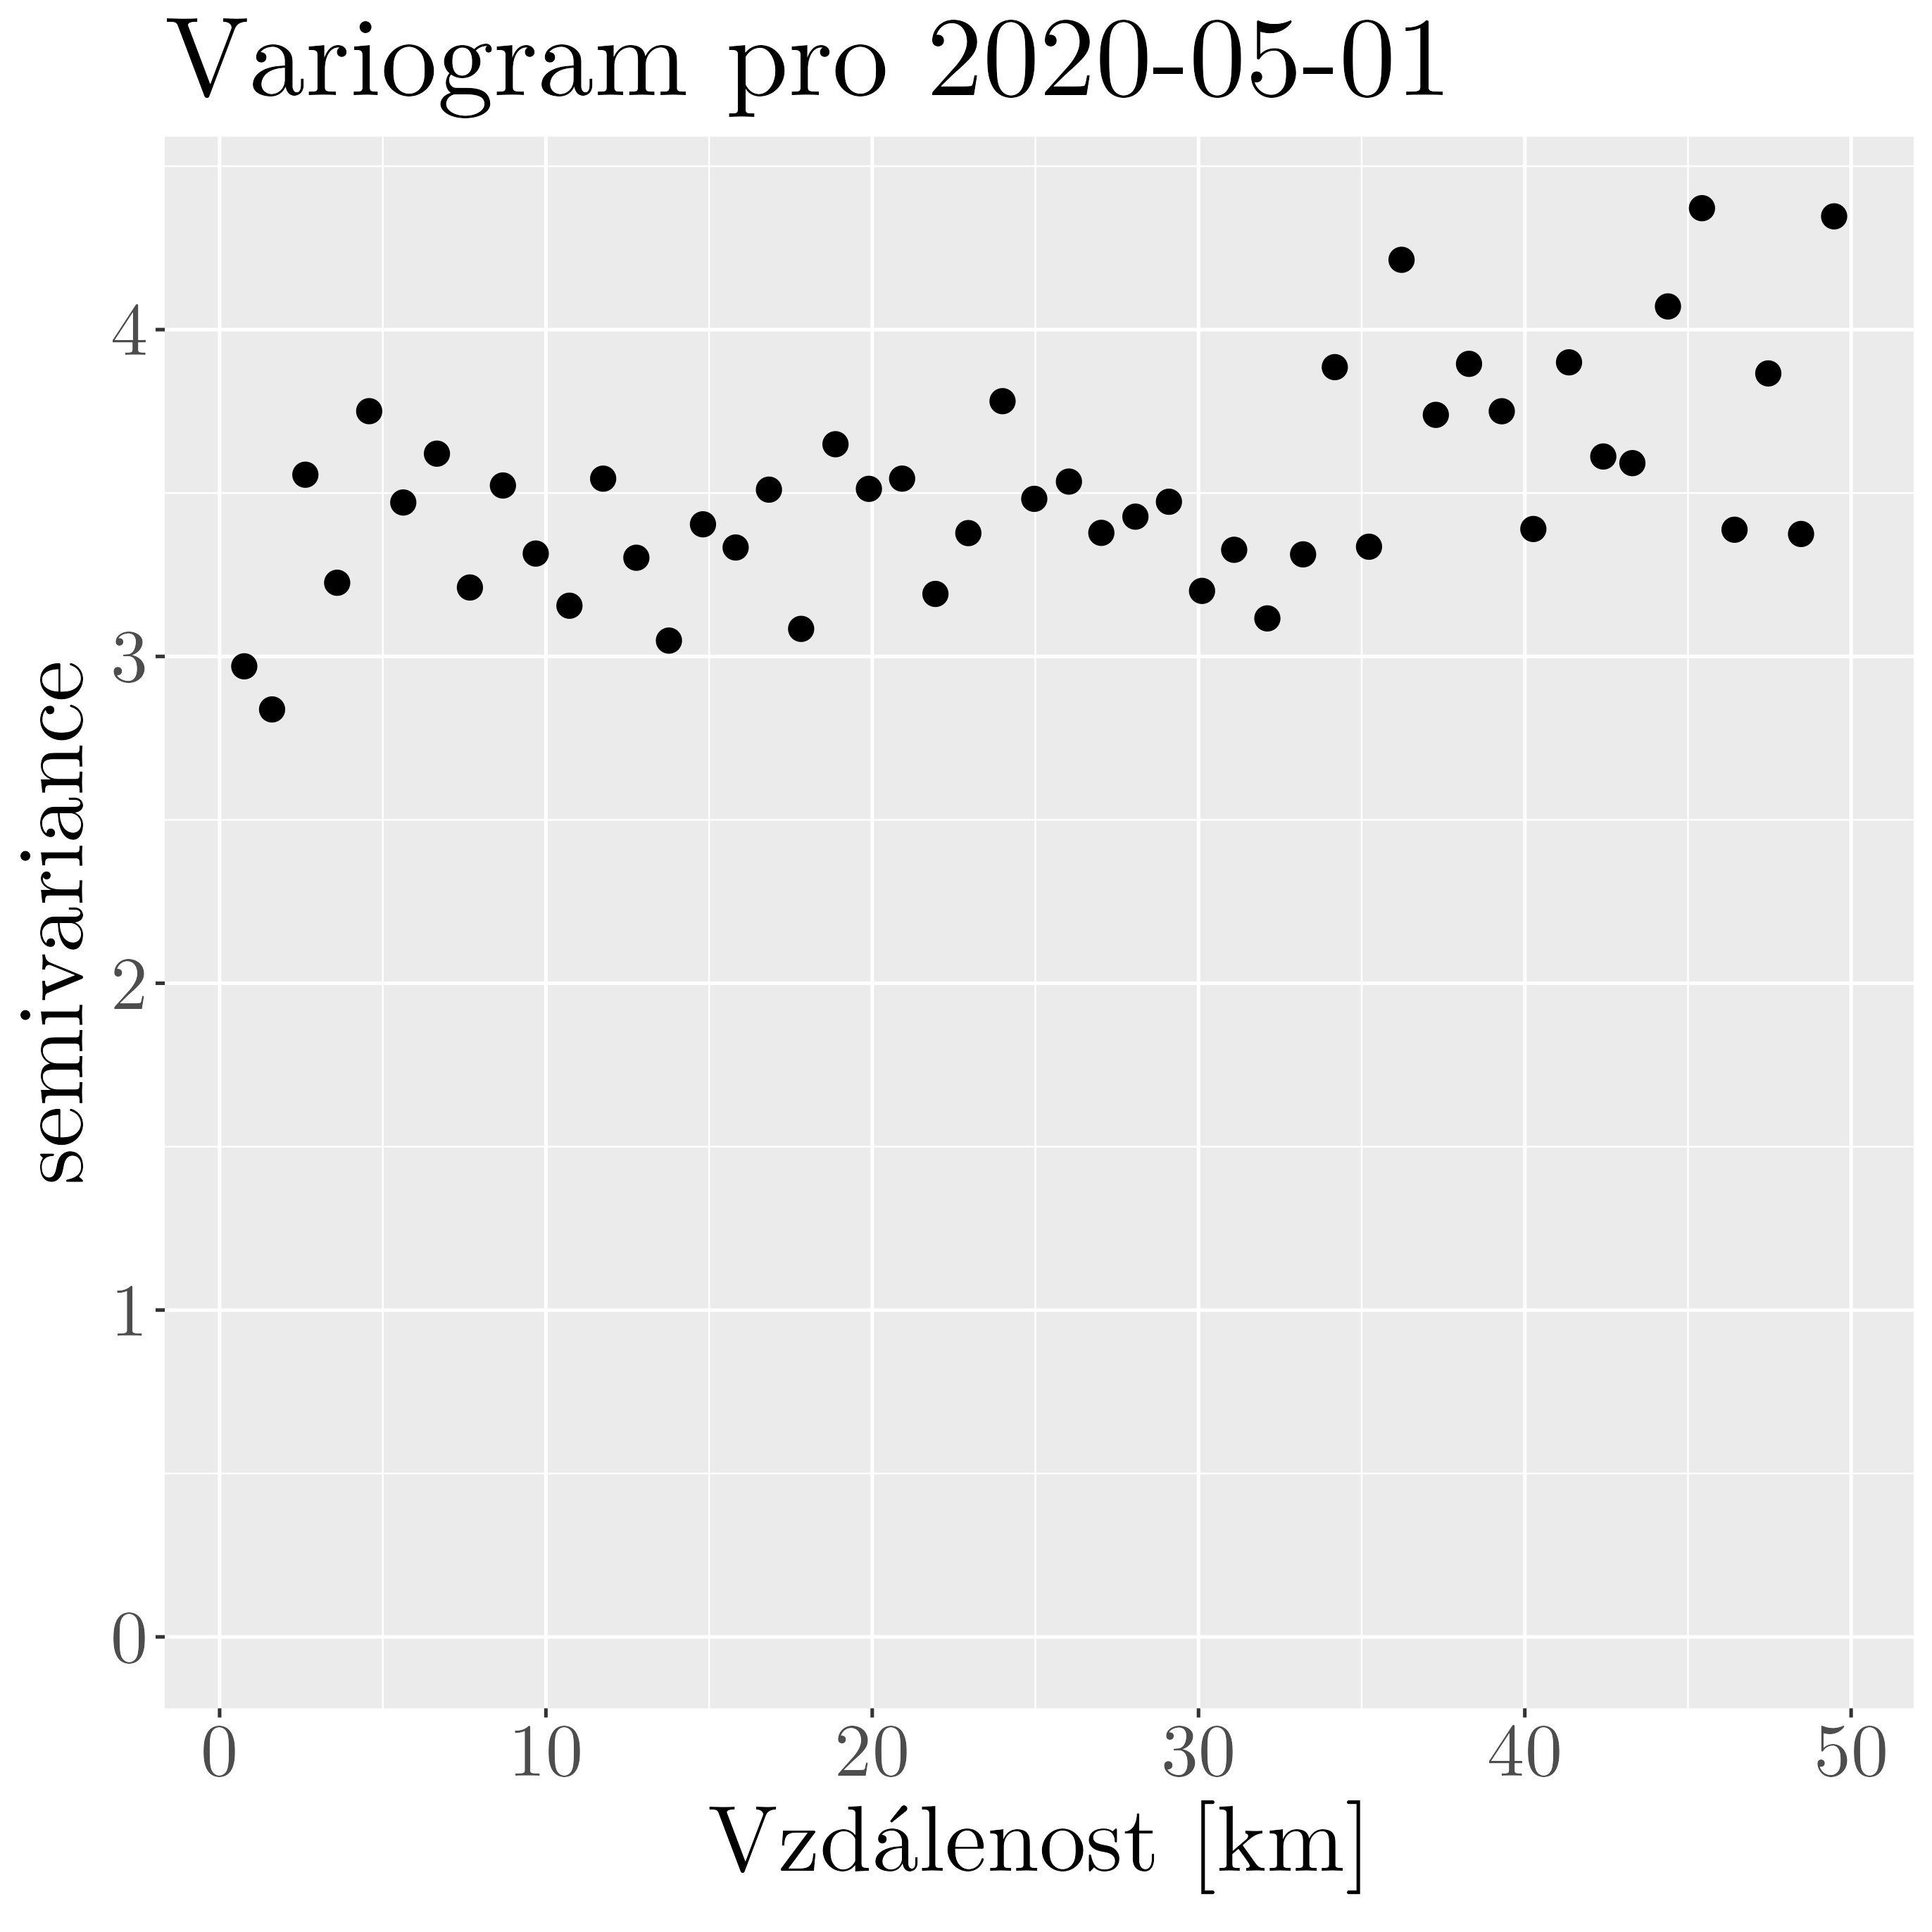
\includegraphics[width=\textwidth]{img/ch2/variograms/variogram_max15cm5.png}
		\caption{}
		\label{fig:variogram5}
	\end{subfigure}
	\hfill
	\begin{subfigure}{0.30\textwidth}
		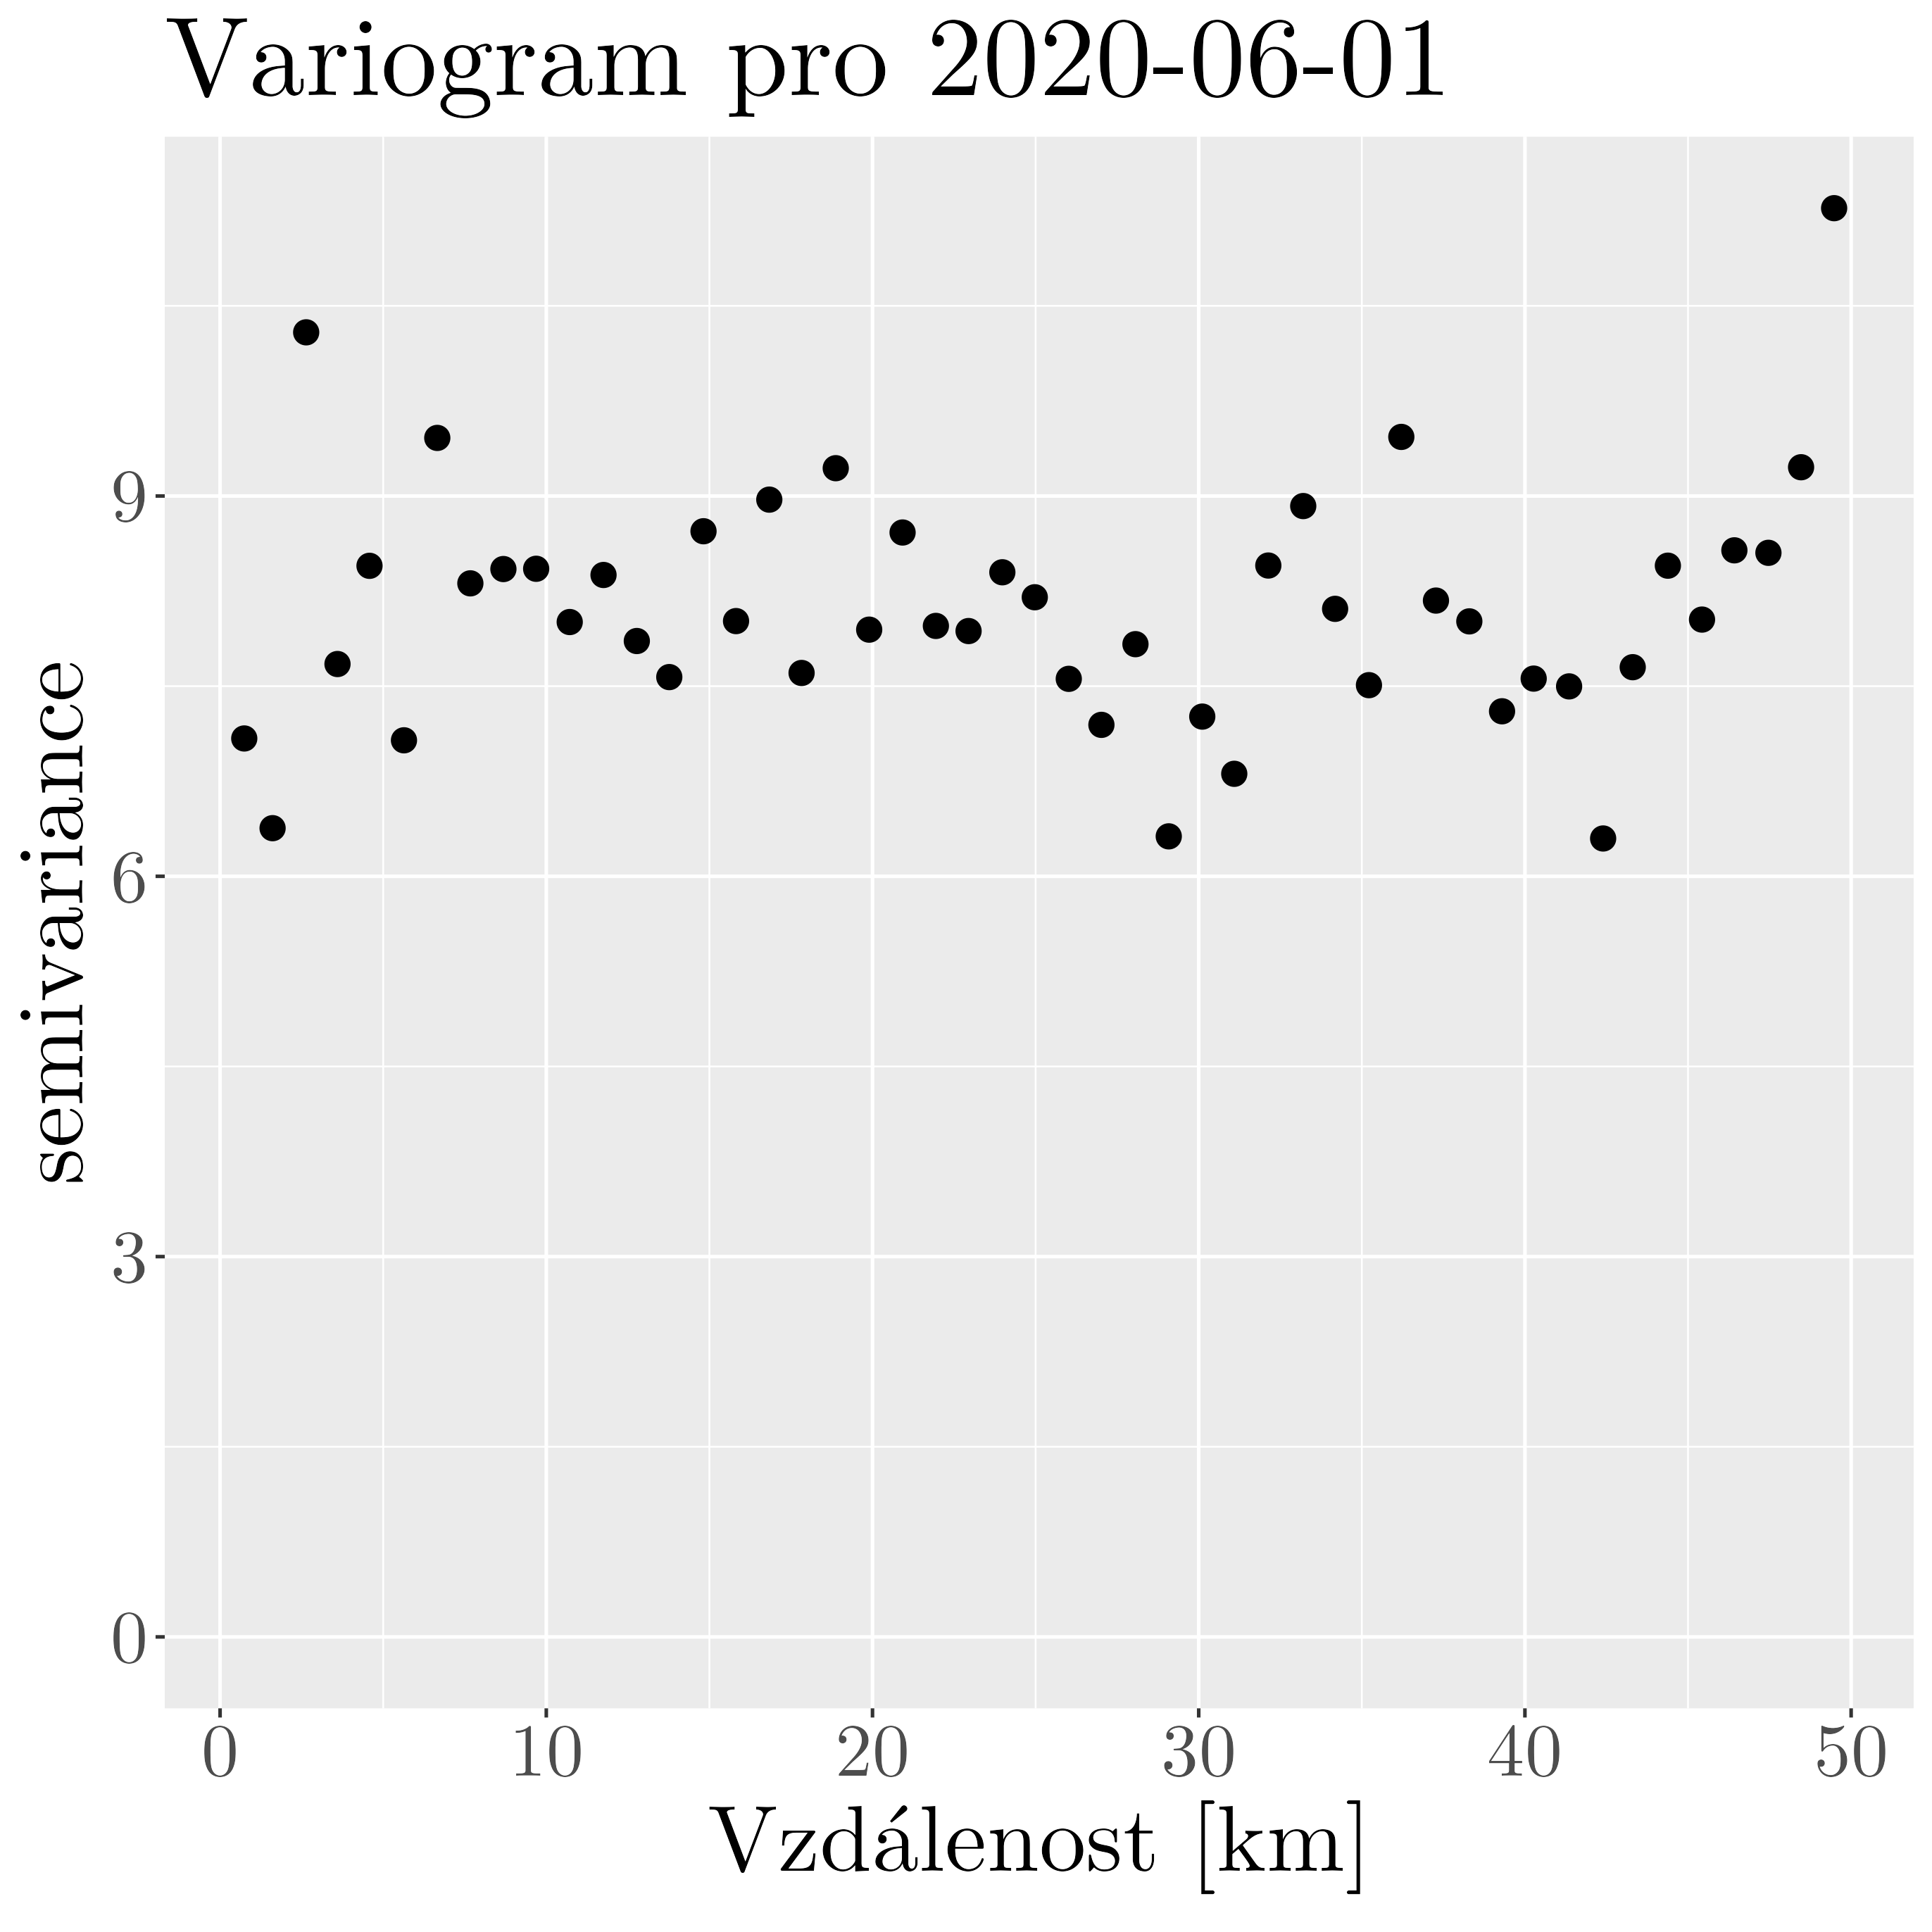
\includegraphics[width=\textwidth]{img/ch2/variograms/variogram_max15cm6.png}
		\caption{}
		\label{fig:variogram6}
	\end{subfigure}
\hfill
	\begin{subfigure}{0.30\textwidth}
		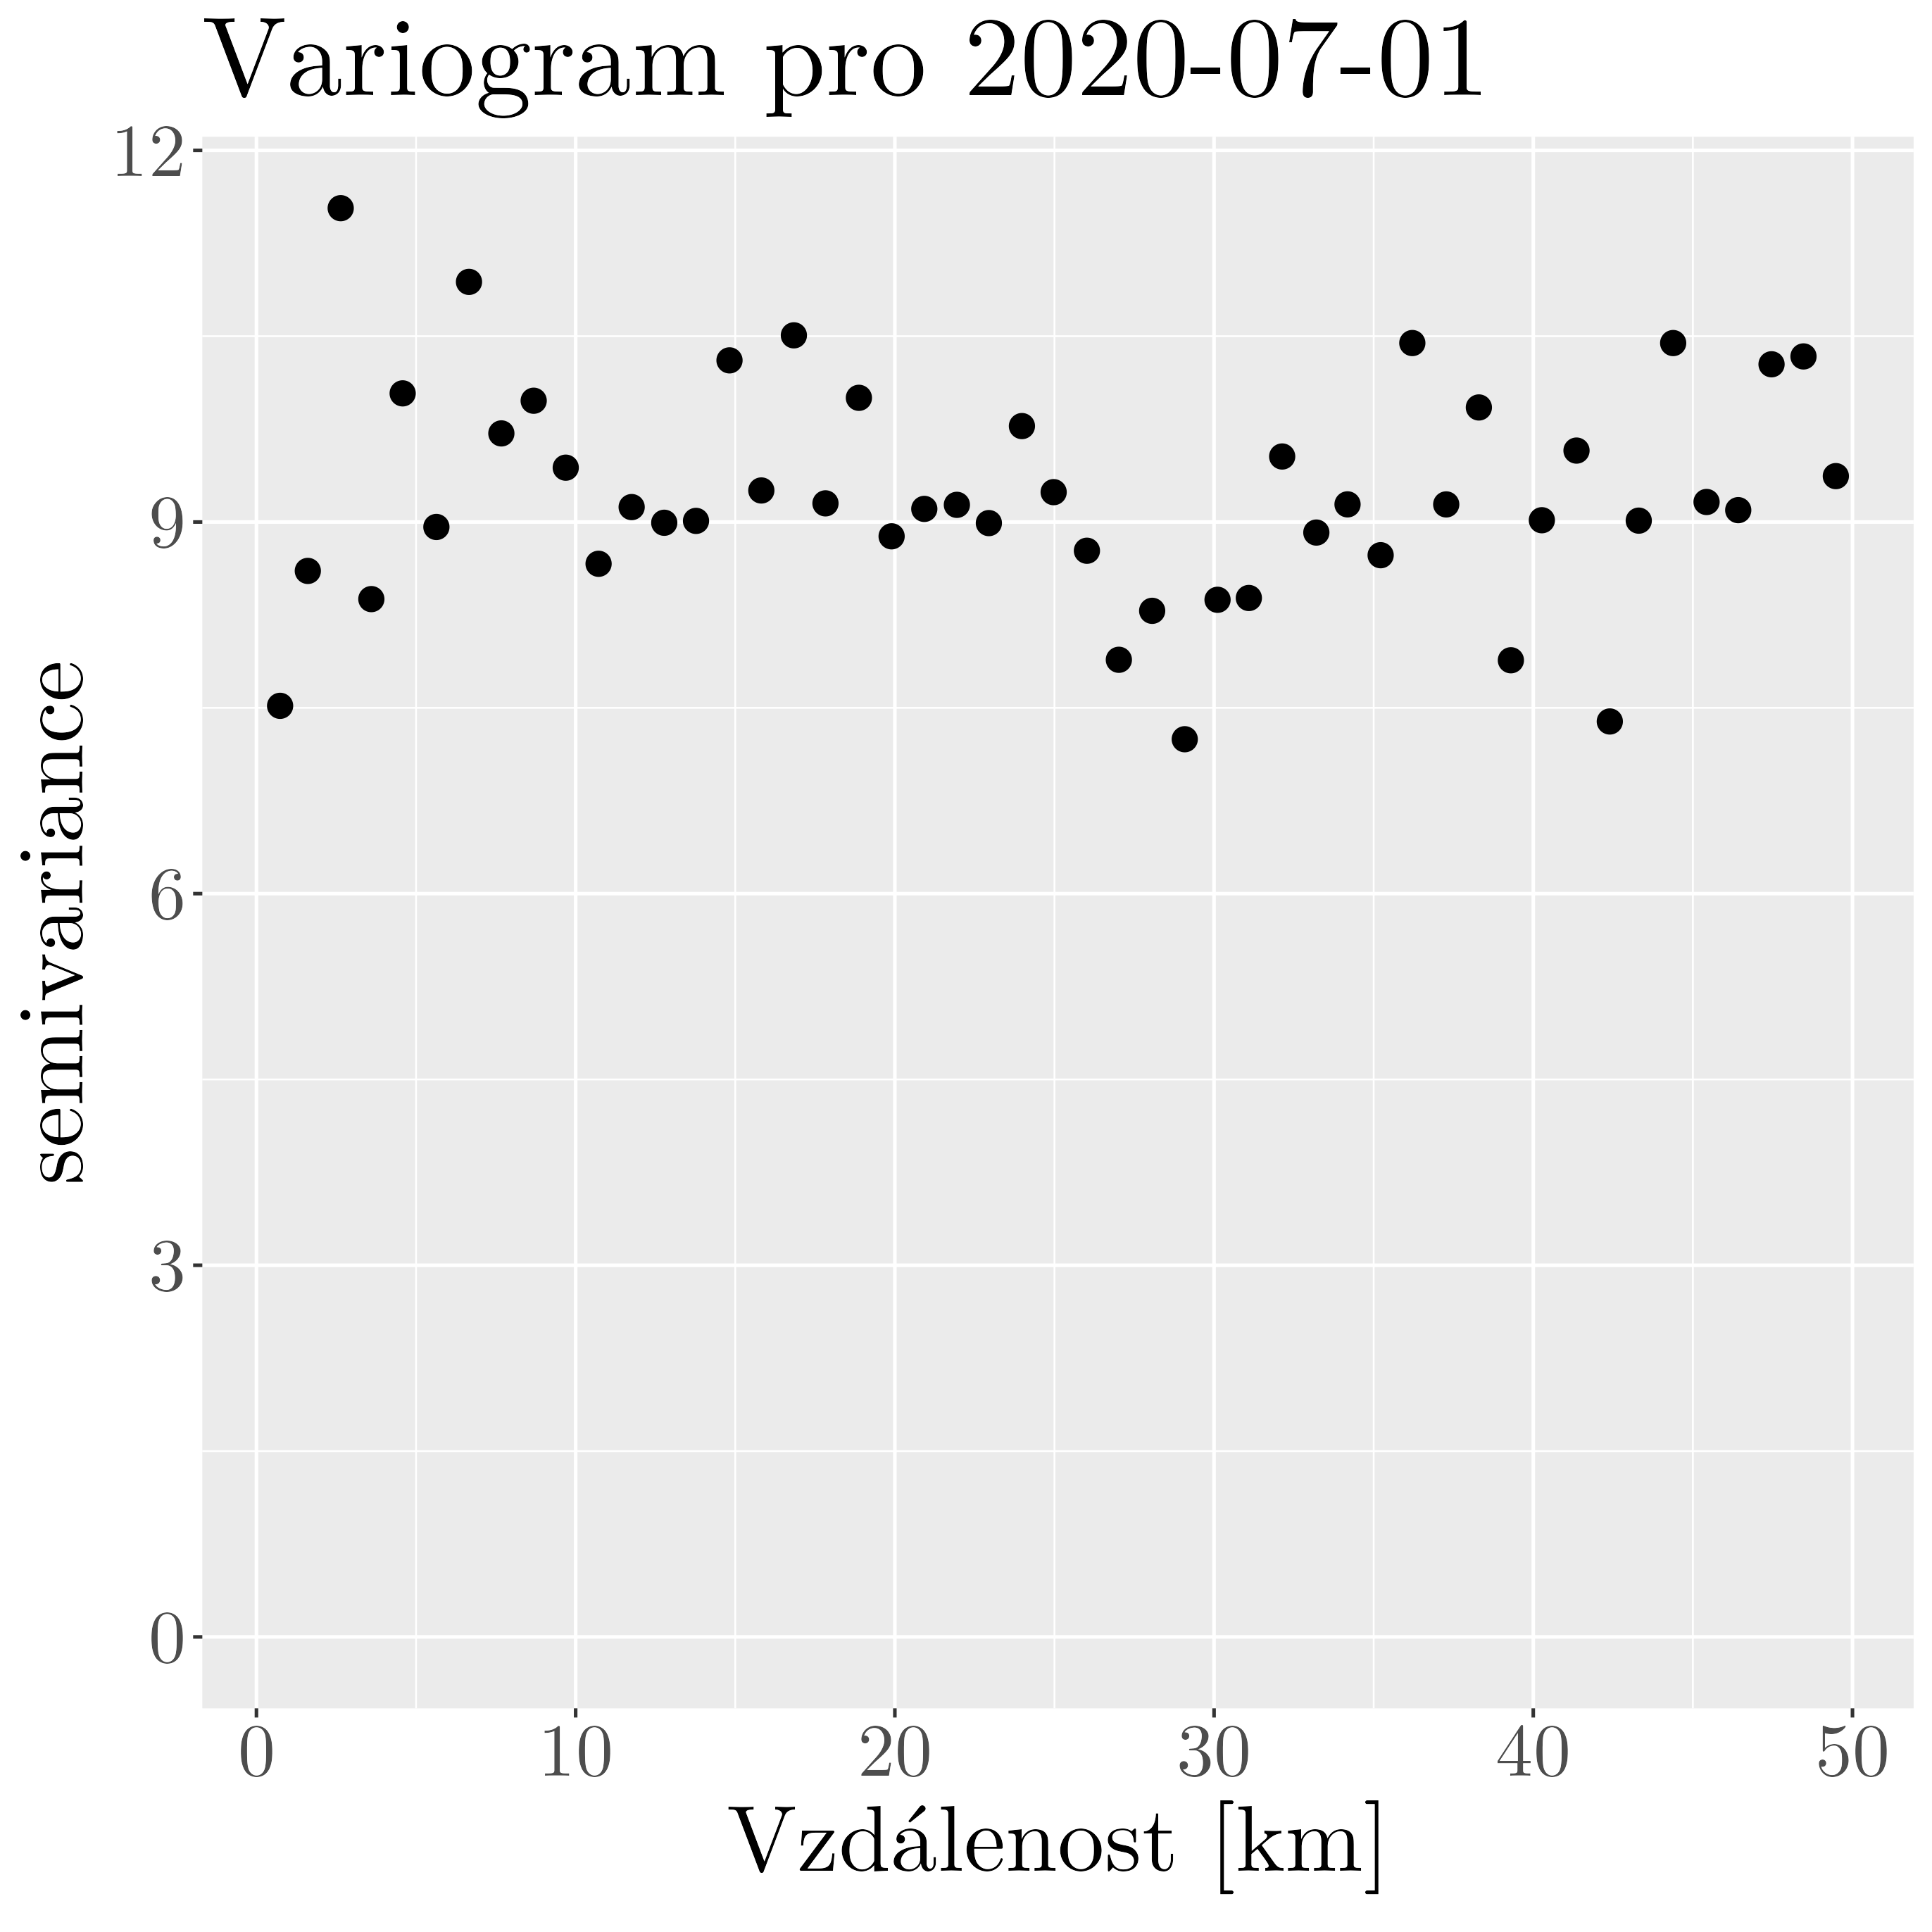
\includegraphics[width=\textwidth]{img/ch2/variograms/variogram_max15cm7.png}
		\caption{}
		\label{fig:variogram7}
	\end{subfigure}
\hfill
	\begin{subfigure}{0.30\textwidth}
		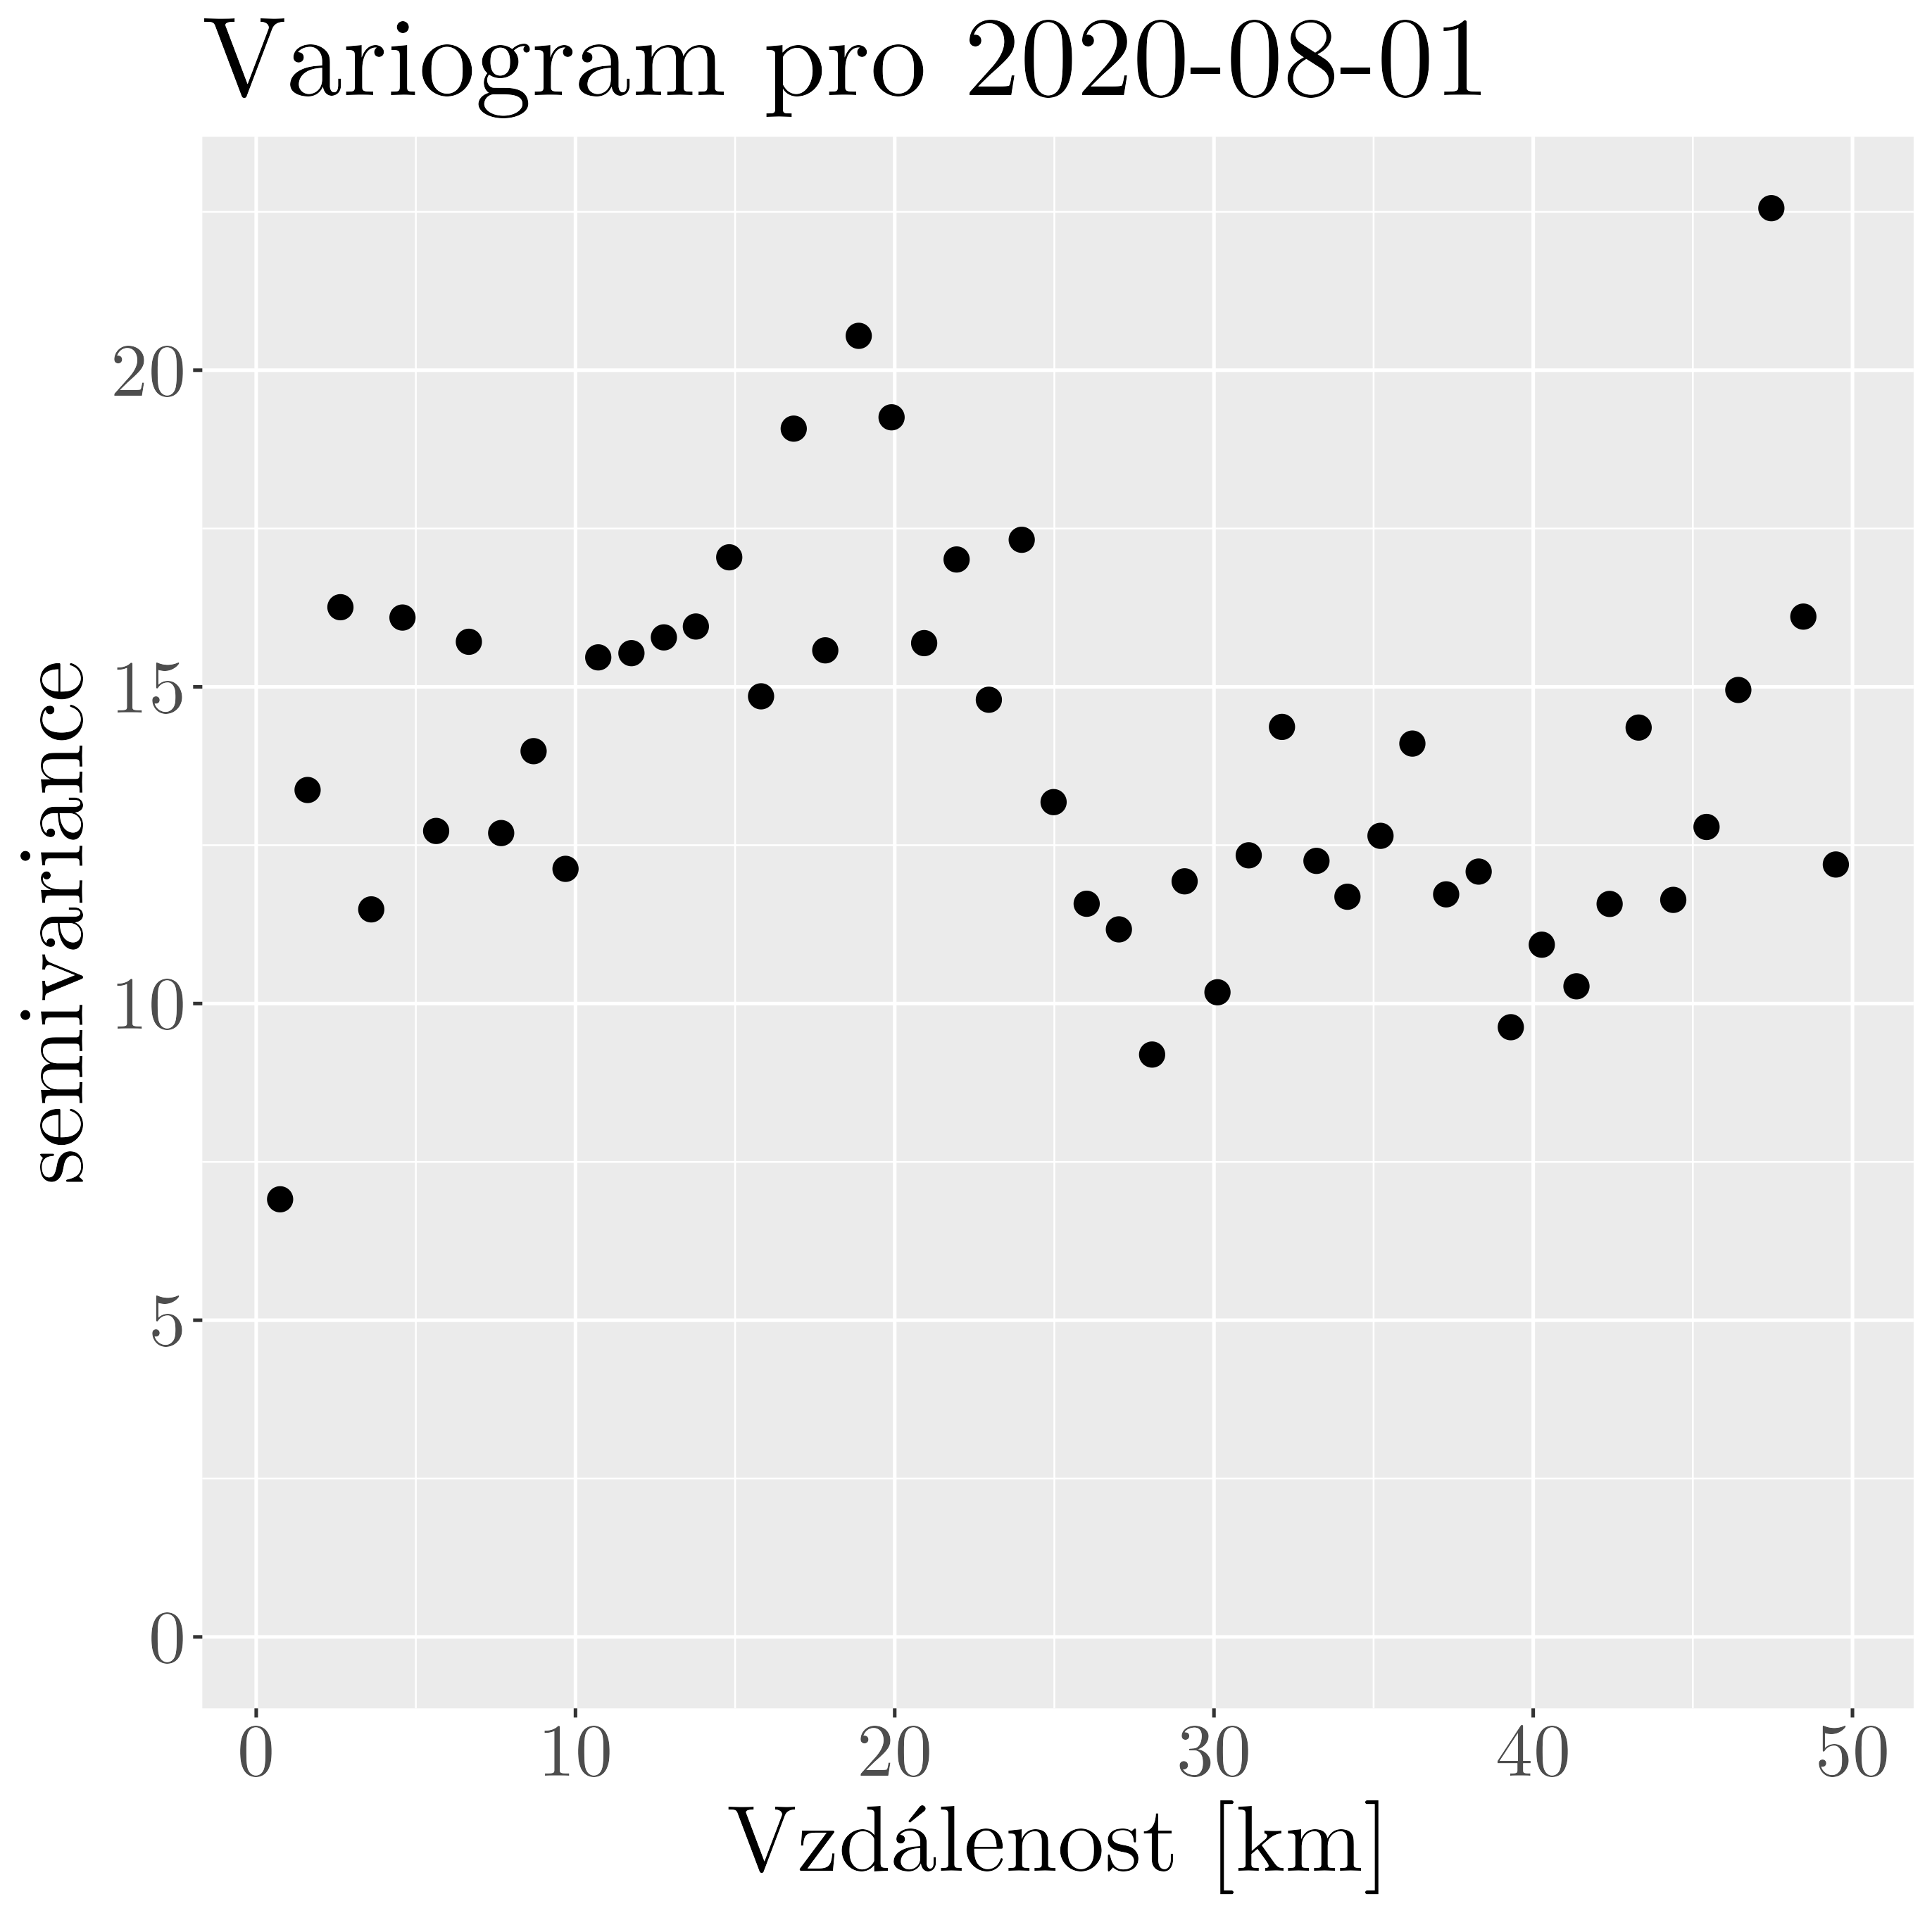
\includegraphics[width=\textwidth]{img/ch2/variograms/variogram_max15cm8.png}
		\caption{}
		\label{fig:variogram8}
	\end{subfigure}
\hfill
	\begin{subfigure}{0.30\textwidth}
		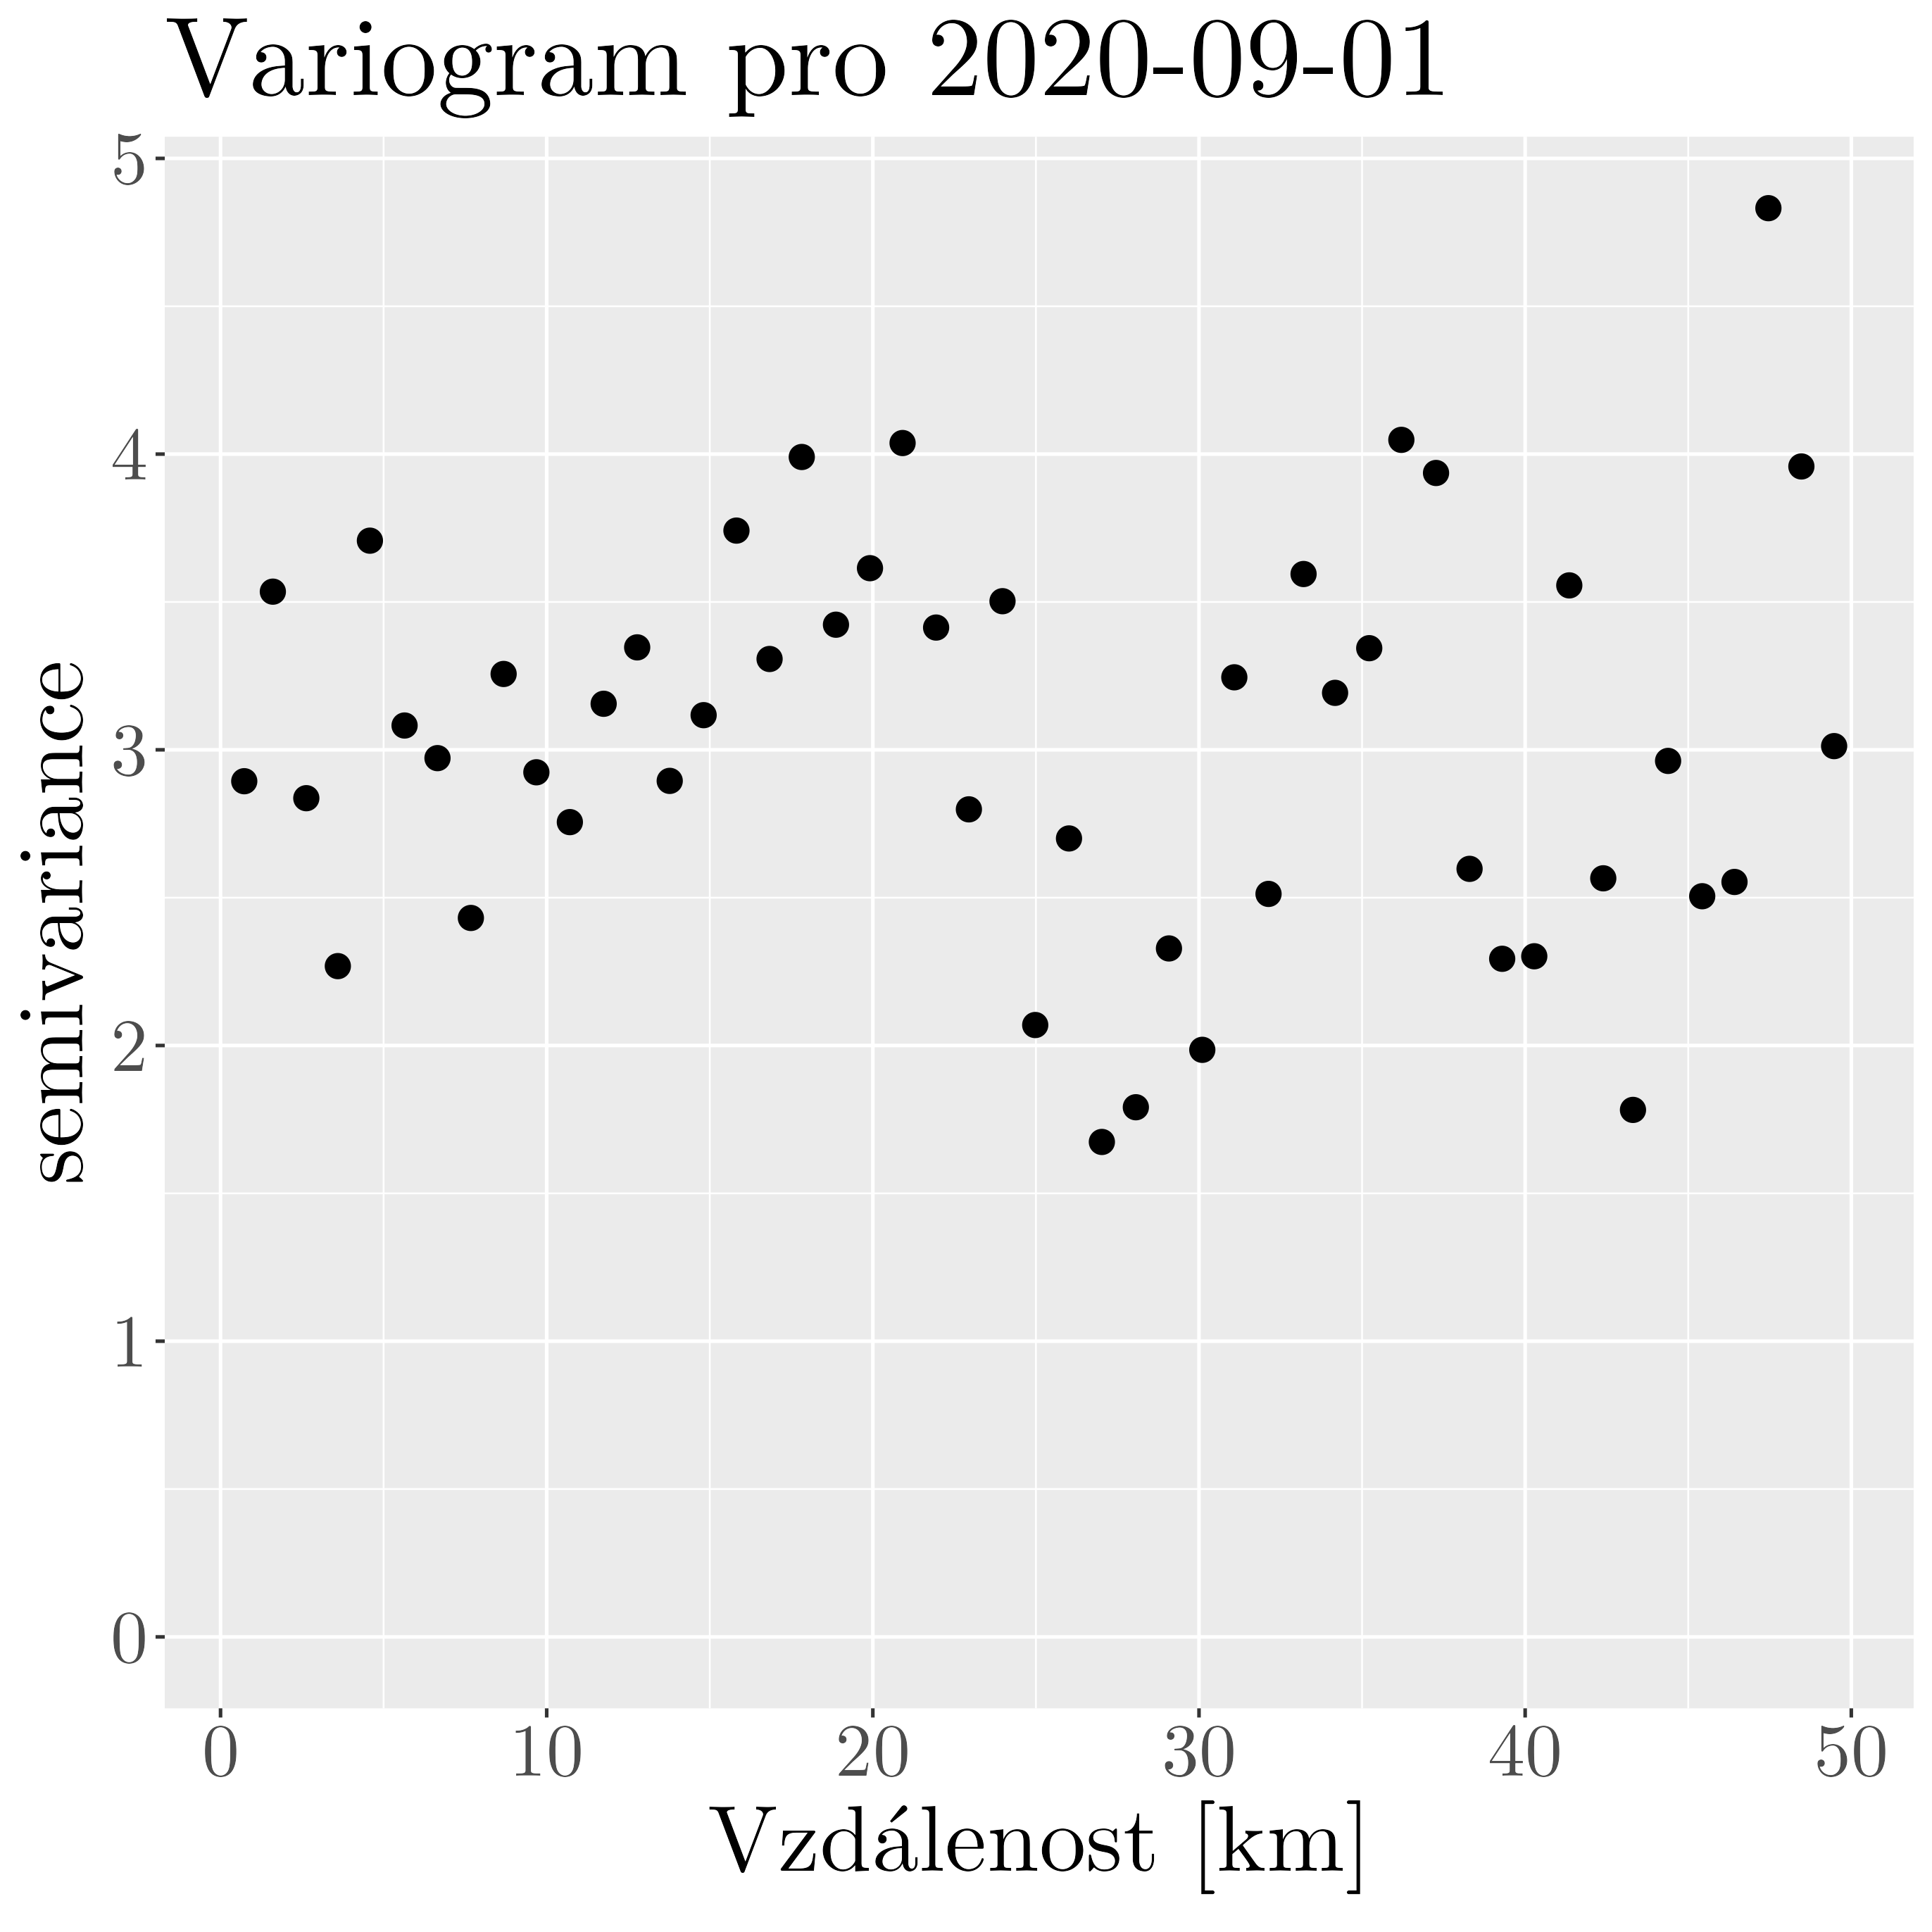
\includegraphics[width=\textwidth]{img/ch2/variograms/variogram_max15cm9.png}
		\caption{}
		\label{fig:variogram9}
	\end{subfigure}
\hfill
	\begin{subfigure}{0.30\textwidth}
		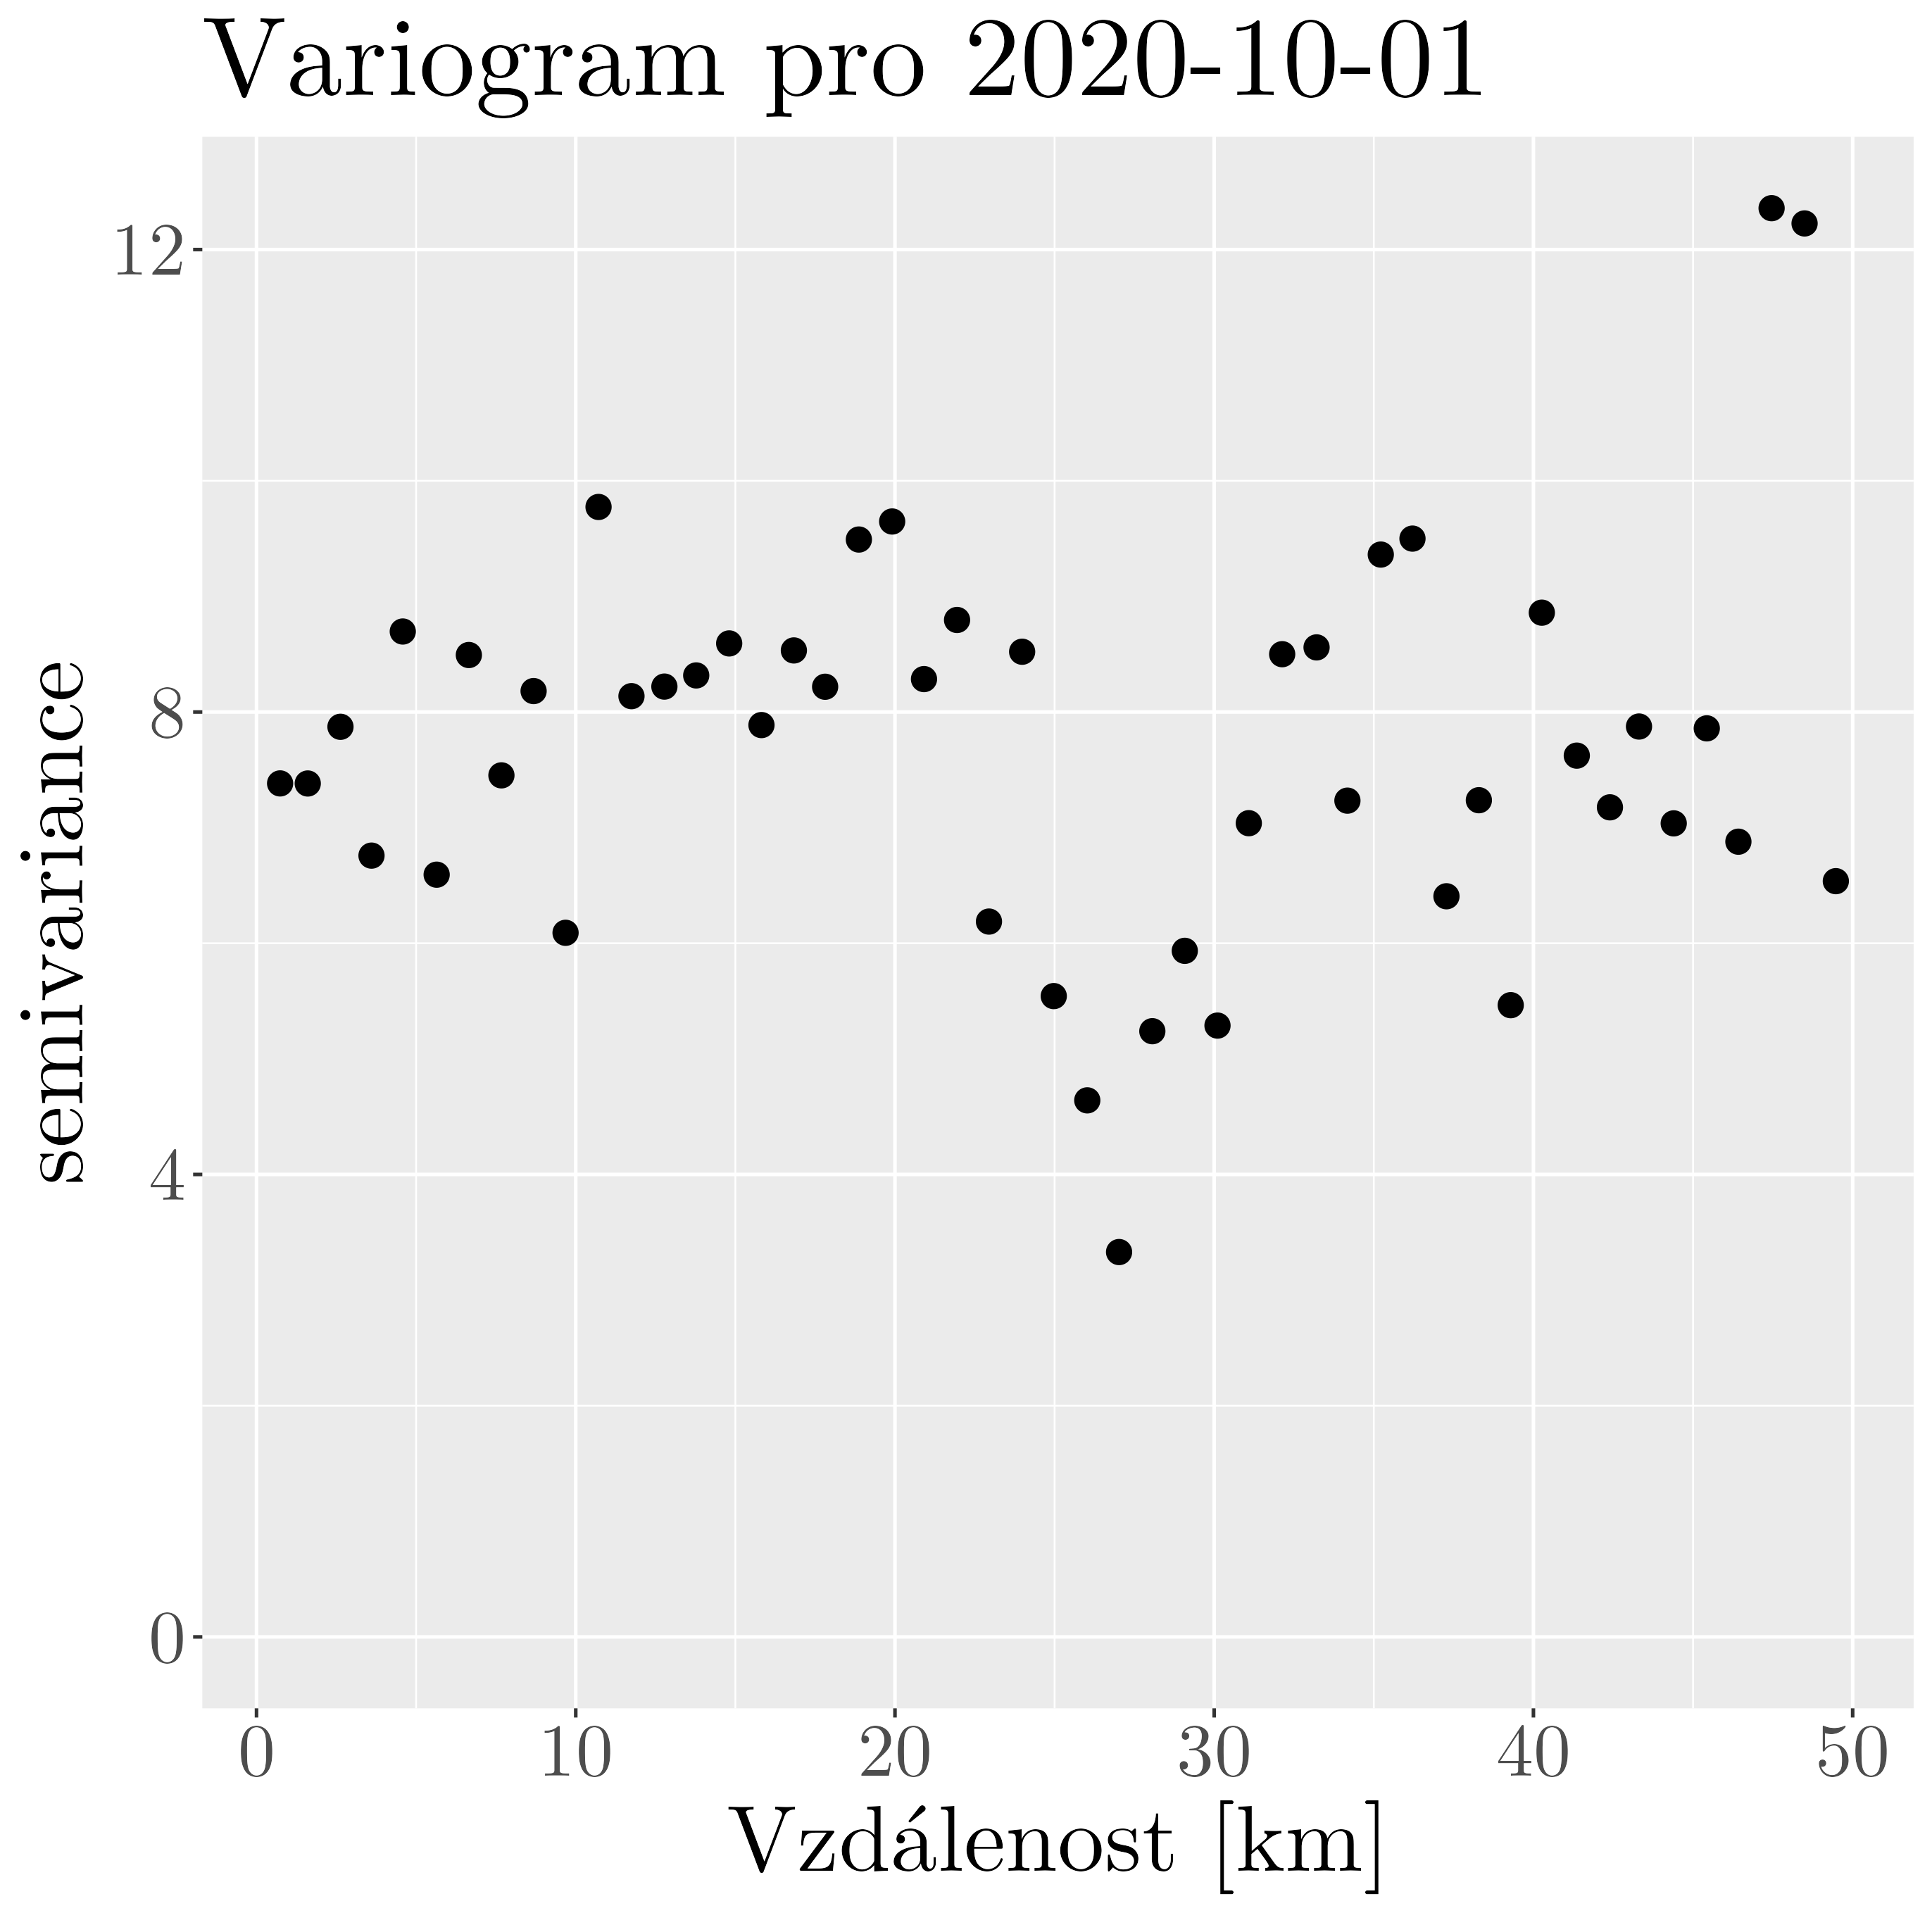
\includegraphics[width=\textwidth]{img/ch2/variograms/variogram_max15cm10.png}
		\caption{}
		\label{fig:variogram10}
	\end{subfigure}
\hfill
	\begin{subfigure}{0.30\textwidth}
		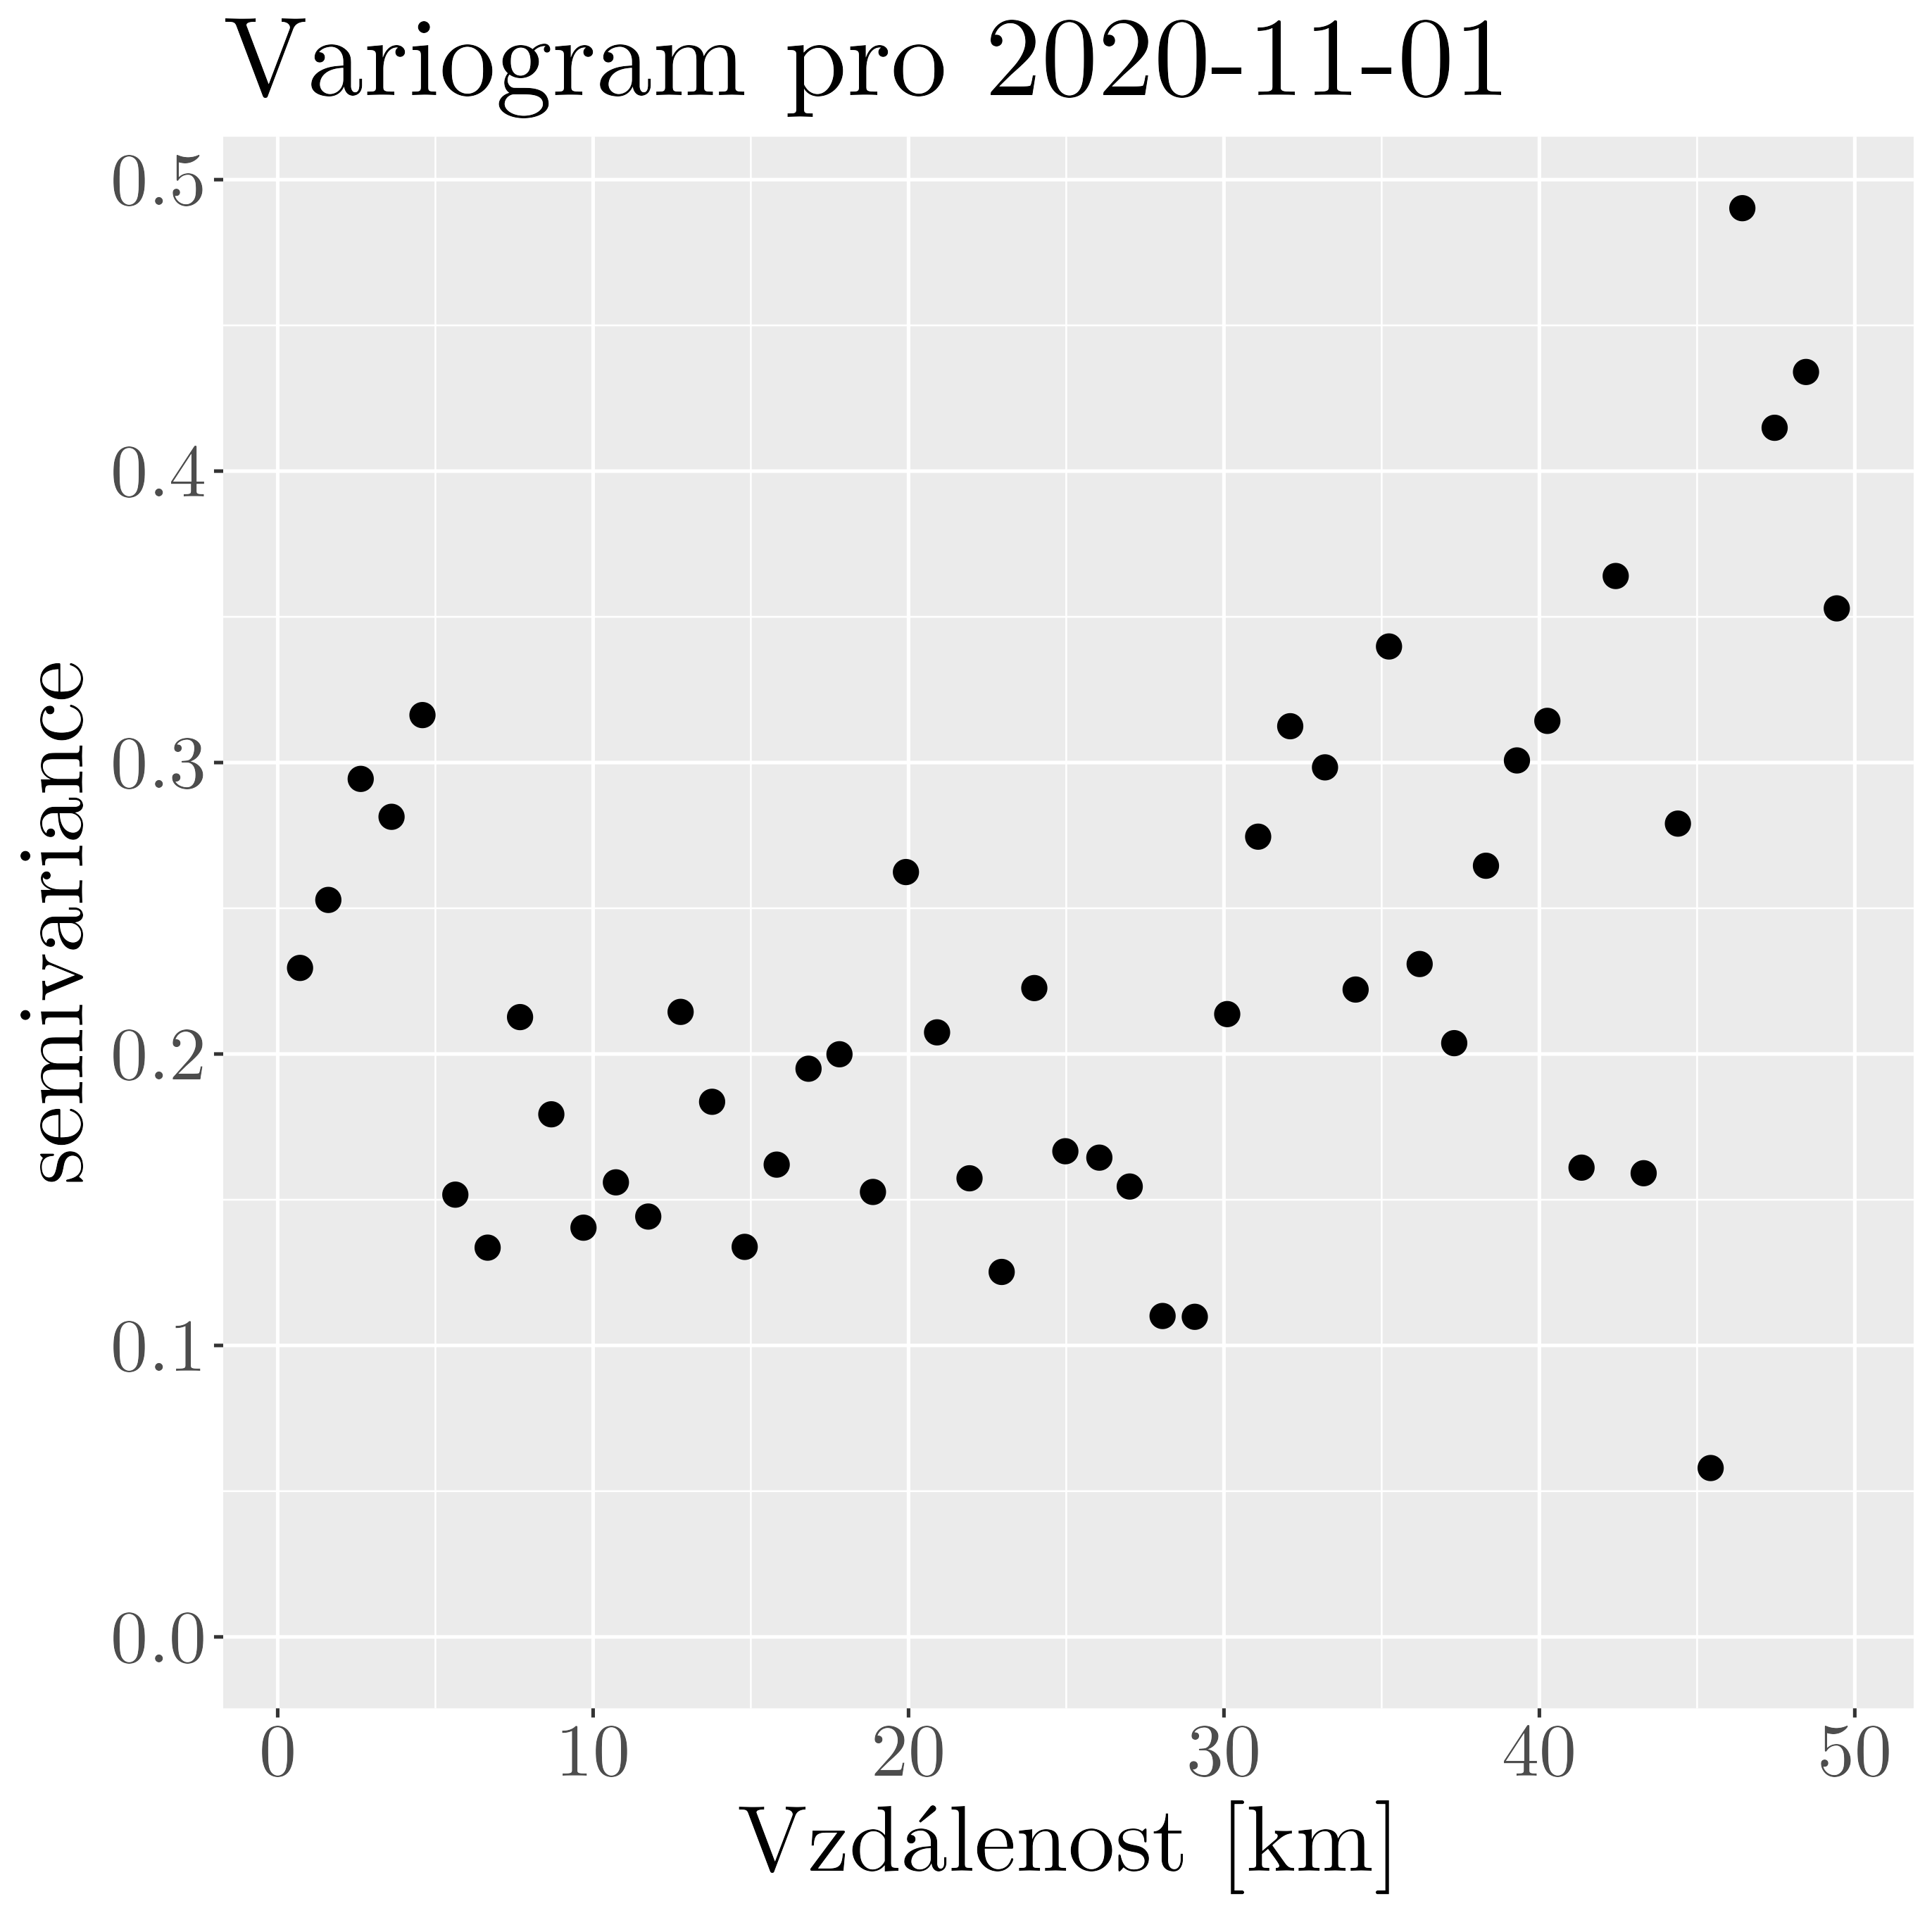
\includegraphics[width=\textwidth]{img/ch2/variograms/variogram_max15cm11.png}
		\caption{}
		\label{fig:variogram11}
	\end{subfigure}
\hfill
	\begin{subfigure}{0.30\textwidth}
		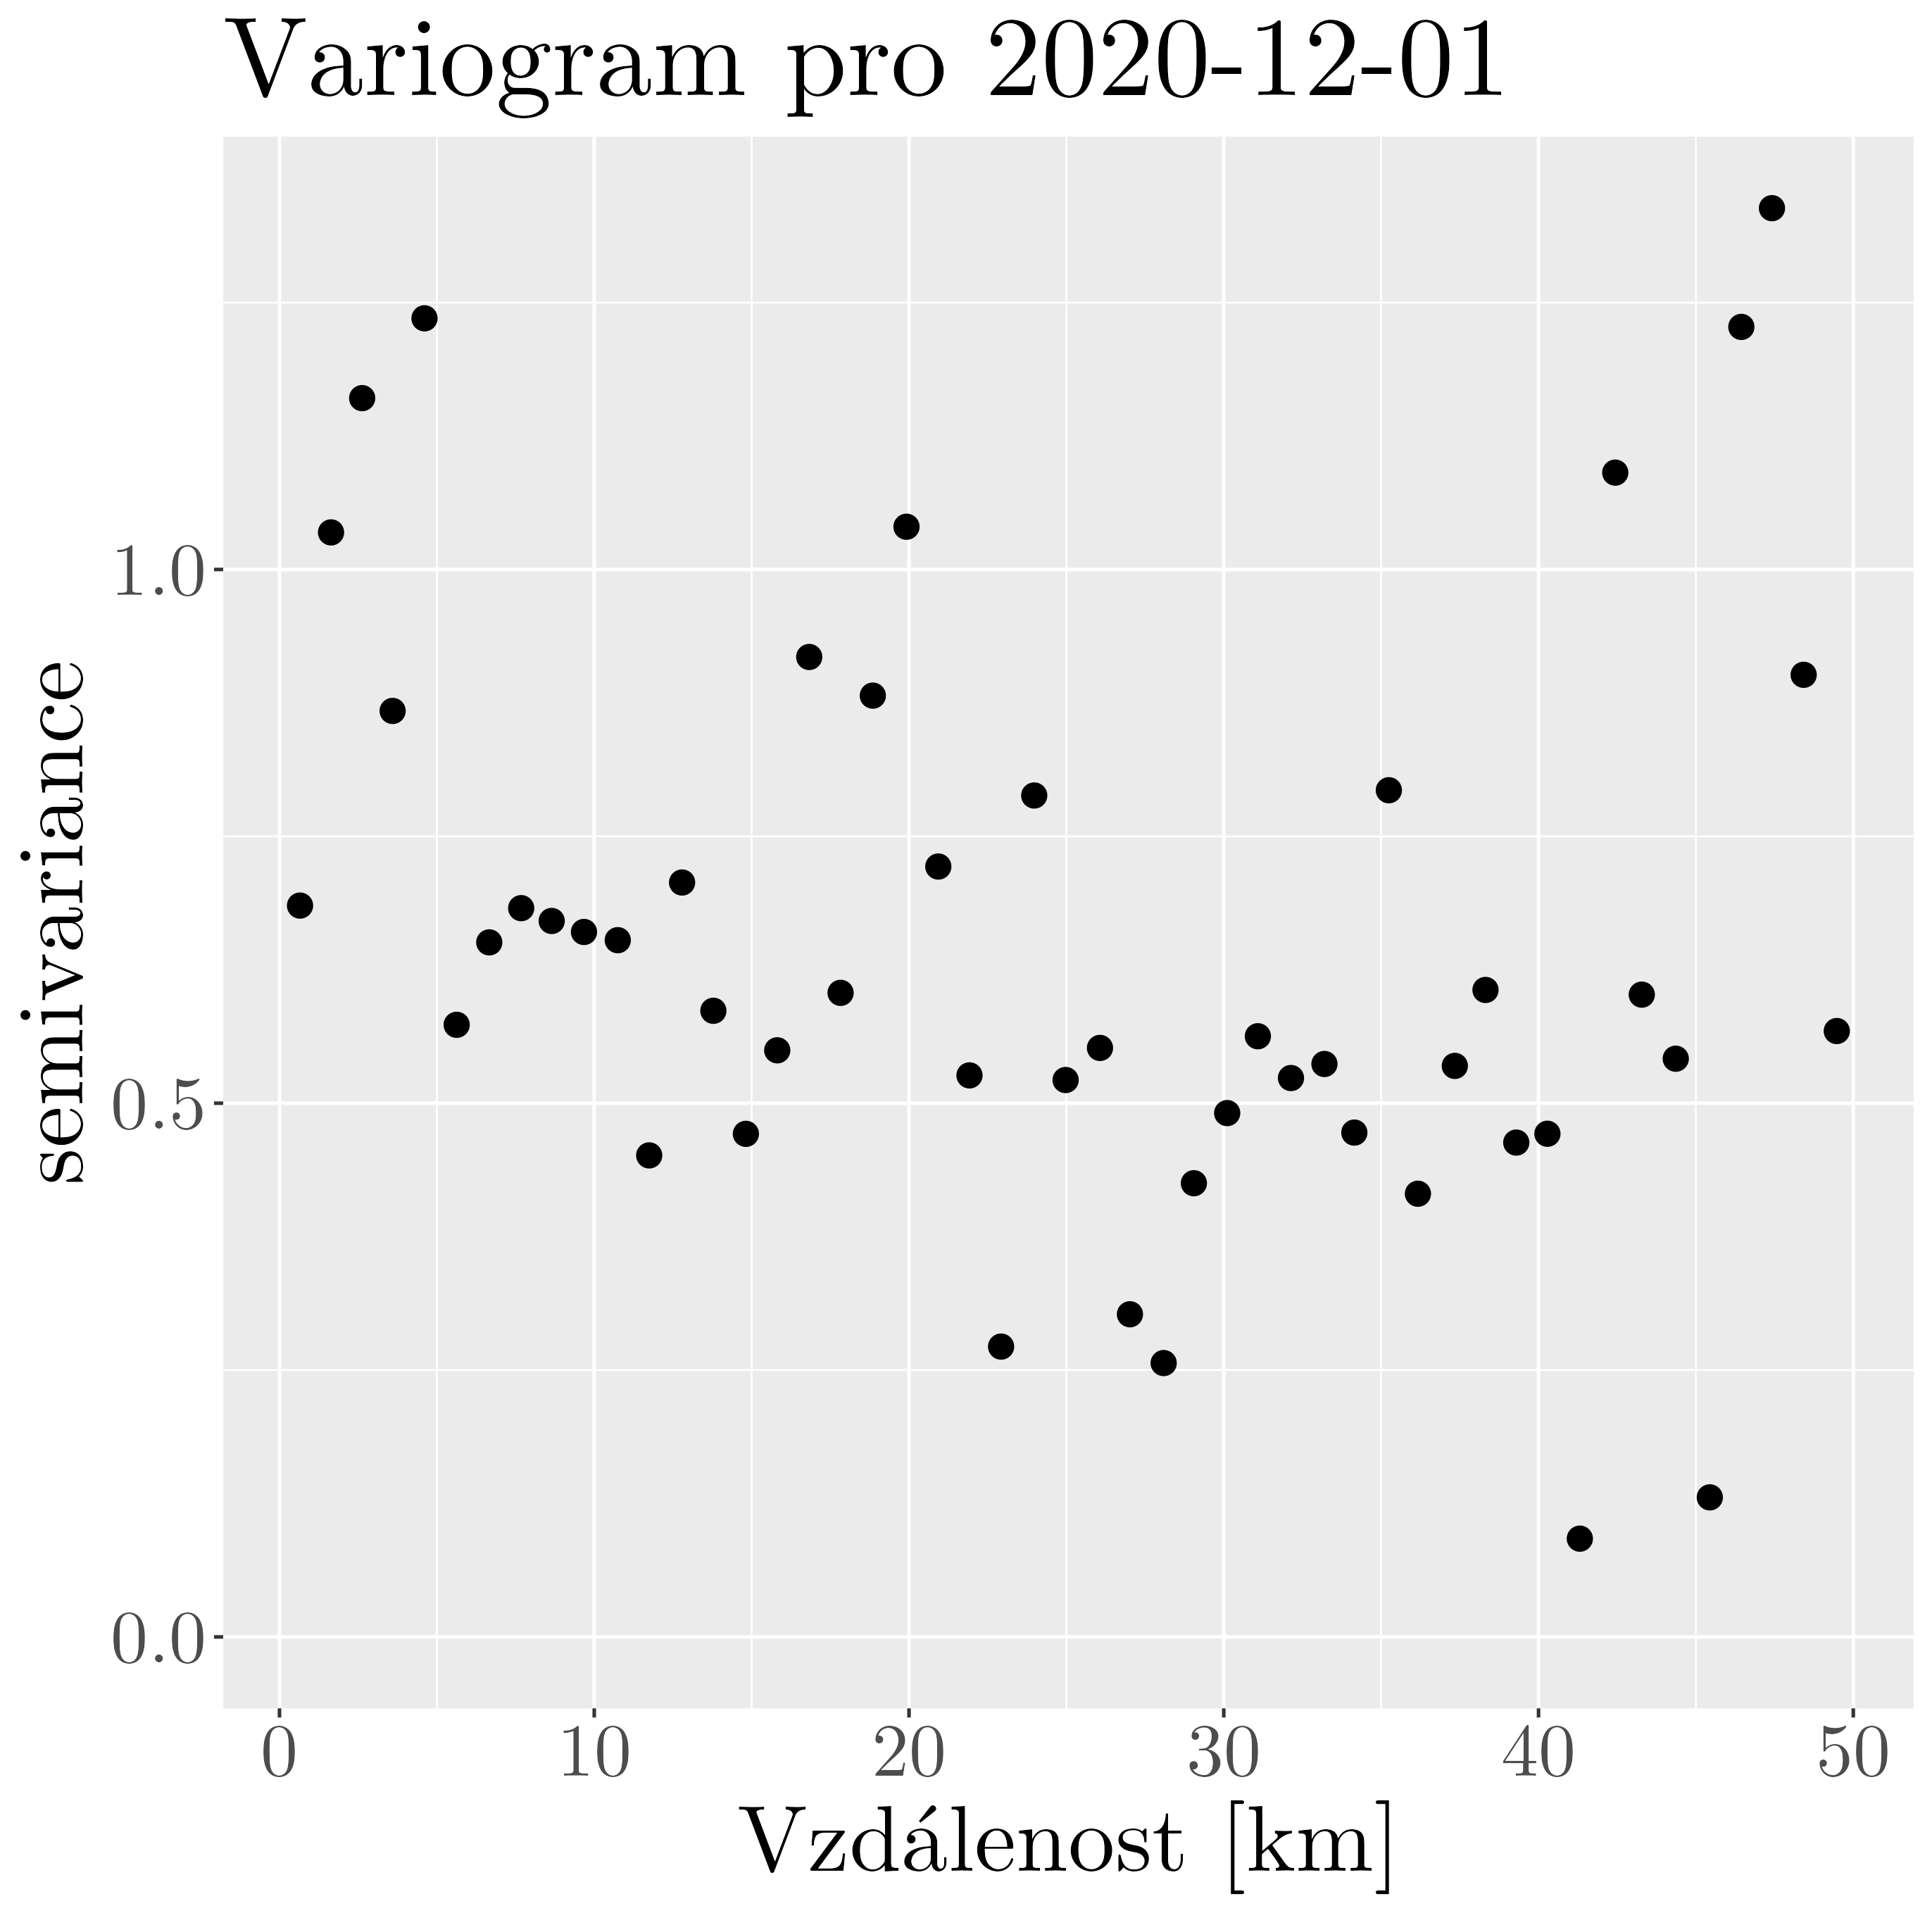
\includegraphics[width=\textwidth]{img/ch2/variograms/variogram_max15cm12.png}
		\caption{}
		\label{fig:variogram12}
	\end{subfigure}
	\caption{Semivariogramy pro jednotlivé první dny měsíců v roce 2020.}
	\label{fig:variograms}
\end{figure}

\subsection{Lineární model se smíšenými efekty}
Pro analýzu vlivu meteorologických proměnných je vhodný lineární model se smíšenými efekty popsaný v kapitole \ref{chap:lme}. Jako náhodný efekt, jehož reálná hodnota pro nás není důležitá, určíme název čidla. Pro všechna čidla a všechny dostupné dny máme kolem 78000 pozorování rozdílu maximální teploty při zemi a ve $\SI{2}{m}$ (konkrétní počet se může lišit, jestliže bereme teplotu v $\SI{0}{cm}$ nebo $\SI{15}{cm}$ nad zemí). Když vyřadíme měření pro která chybí některá data z meteorologický stanic (typicky oblačnost ze stanice Churáňov) a poslední čtyři dny měření, kdy máme data z menšího množství čidel, tak máme 63000 měření.

Zpracovávaná data mají šest prediktorů: insolace, srážky za poslední hodinu, celková sněhová pokrývka, oblačnost, rychlost větru a půdní vlhkost. Oblačnost nabývá fixní hodnot, je vyjádřena v osminách celkové oblačnosti, nahrazená data z ERA5 jsou vyjádřena v procentech, všechny hodnoty tedy převedeme do intervalu $0$ až $1$. Rychlost větru je měřená v celočíselných násobcích $\SI{3.6}{m/s}$. Ostatní prediktory, stejně jako rozdíl mezi teplotami při povrchu země který se snažíme vysvětlit, jsou spojité proměnné. 

Pro výpočet lineárního modelu se smíšenými efekty použijeme funkci \texttt{lme} z balíčku \texttt{nlme} programovacího jazyka \texttt{R}.

Pro každý model budeme ověřovat předpoklady, nyní krátce ilustrujeme problémy s kterými se budeme v kapitole \ref{chap:ch3} potýkat na jednom modelu. Pracujme tedy s maximální denní teplotou ve výšce $\SI{15}{cm}$ a jejím rozdílem od teploty naměřené ve $\SI{2}{m}$. Porovnáme mezi sebou transformace proměnné kterou se snažíme vysvětlit a to bez transformace, s logaritmem, odmocninou a třetí odmocninou. Zároveň data mají silnou autokorelaci a tudíž, jak bylo popsáno v kapitole \ref{chap:lme} použijeme pro autokorelační strukturu model ARMA s parametry $p=2$ a $q=2$ (tyto hodnoty byly vybrány vyzkoušením několika kombinací). Na obrázcích \ref{fig:qq} vidíme kvantil-kvantilový graf pro jednotlivé transformace. Hodnoty rozdílu teplot jsou ovšem i záporné tudíž místo jednoduchého logaritmu použijeme transformaci \eqref{eq:logtrans}. Podobně ošetříme záporné hodnoty i pro ostatní transformace, jako například 3. odmocninu \eqref{eq:curttrans}. V datech se objevují i hodnoty rozdílu teplot $\Delta t=0$ pro které nemůžeme spočítat logaritmus. Jde ovšem o hodnoty pouze blízké nule, způsobené konečnou přesností čidel, tudíž na tyto hodnoty aplikujeme funkci \texttt{jitter} a tím je odlišíme od nuly a následně provedeme transformaci.

\begin{gather*}
	T \mapsto \mathrm{sign}(T)\cdot \ln\left|T\right| \label{eq:logtrans}\\
	T \mapsto \mathrm{sign}(T)\cdot \sqrt[3]{\left|T\right|} \label{eq:curttrans}
\end{gather*}

\begin{figure}
	\centering
	\begin{subfigure}{0.45\textwidth}
  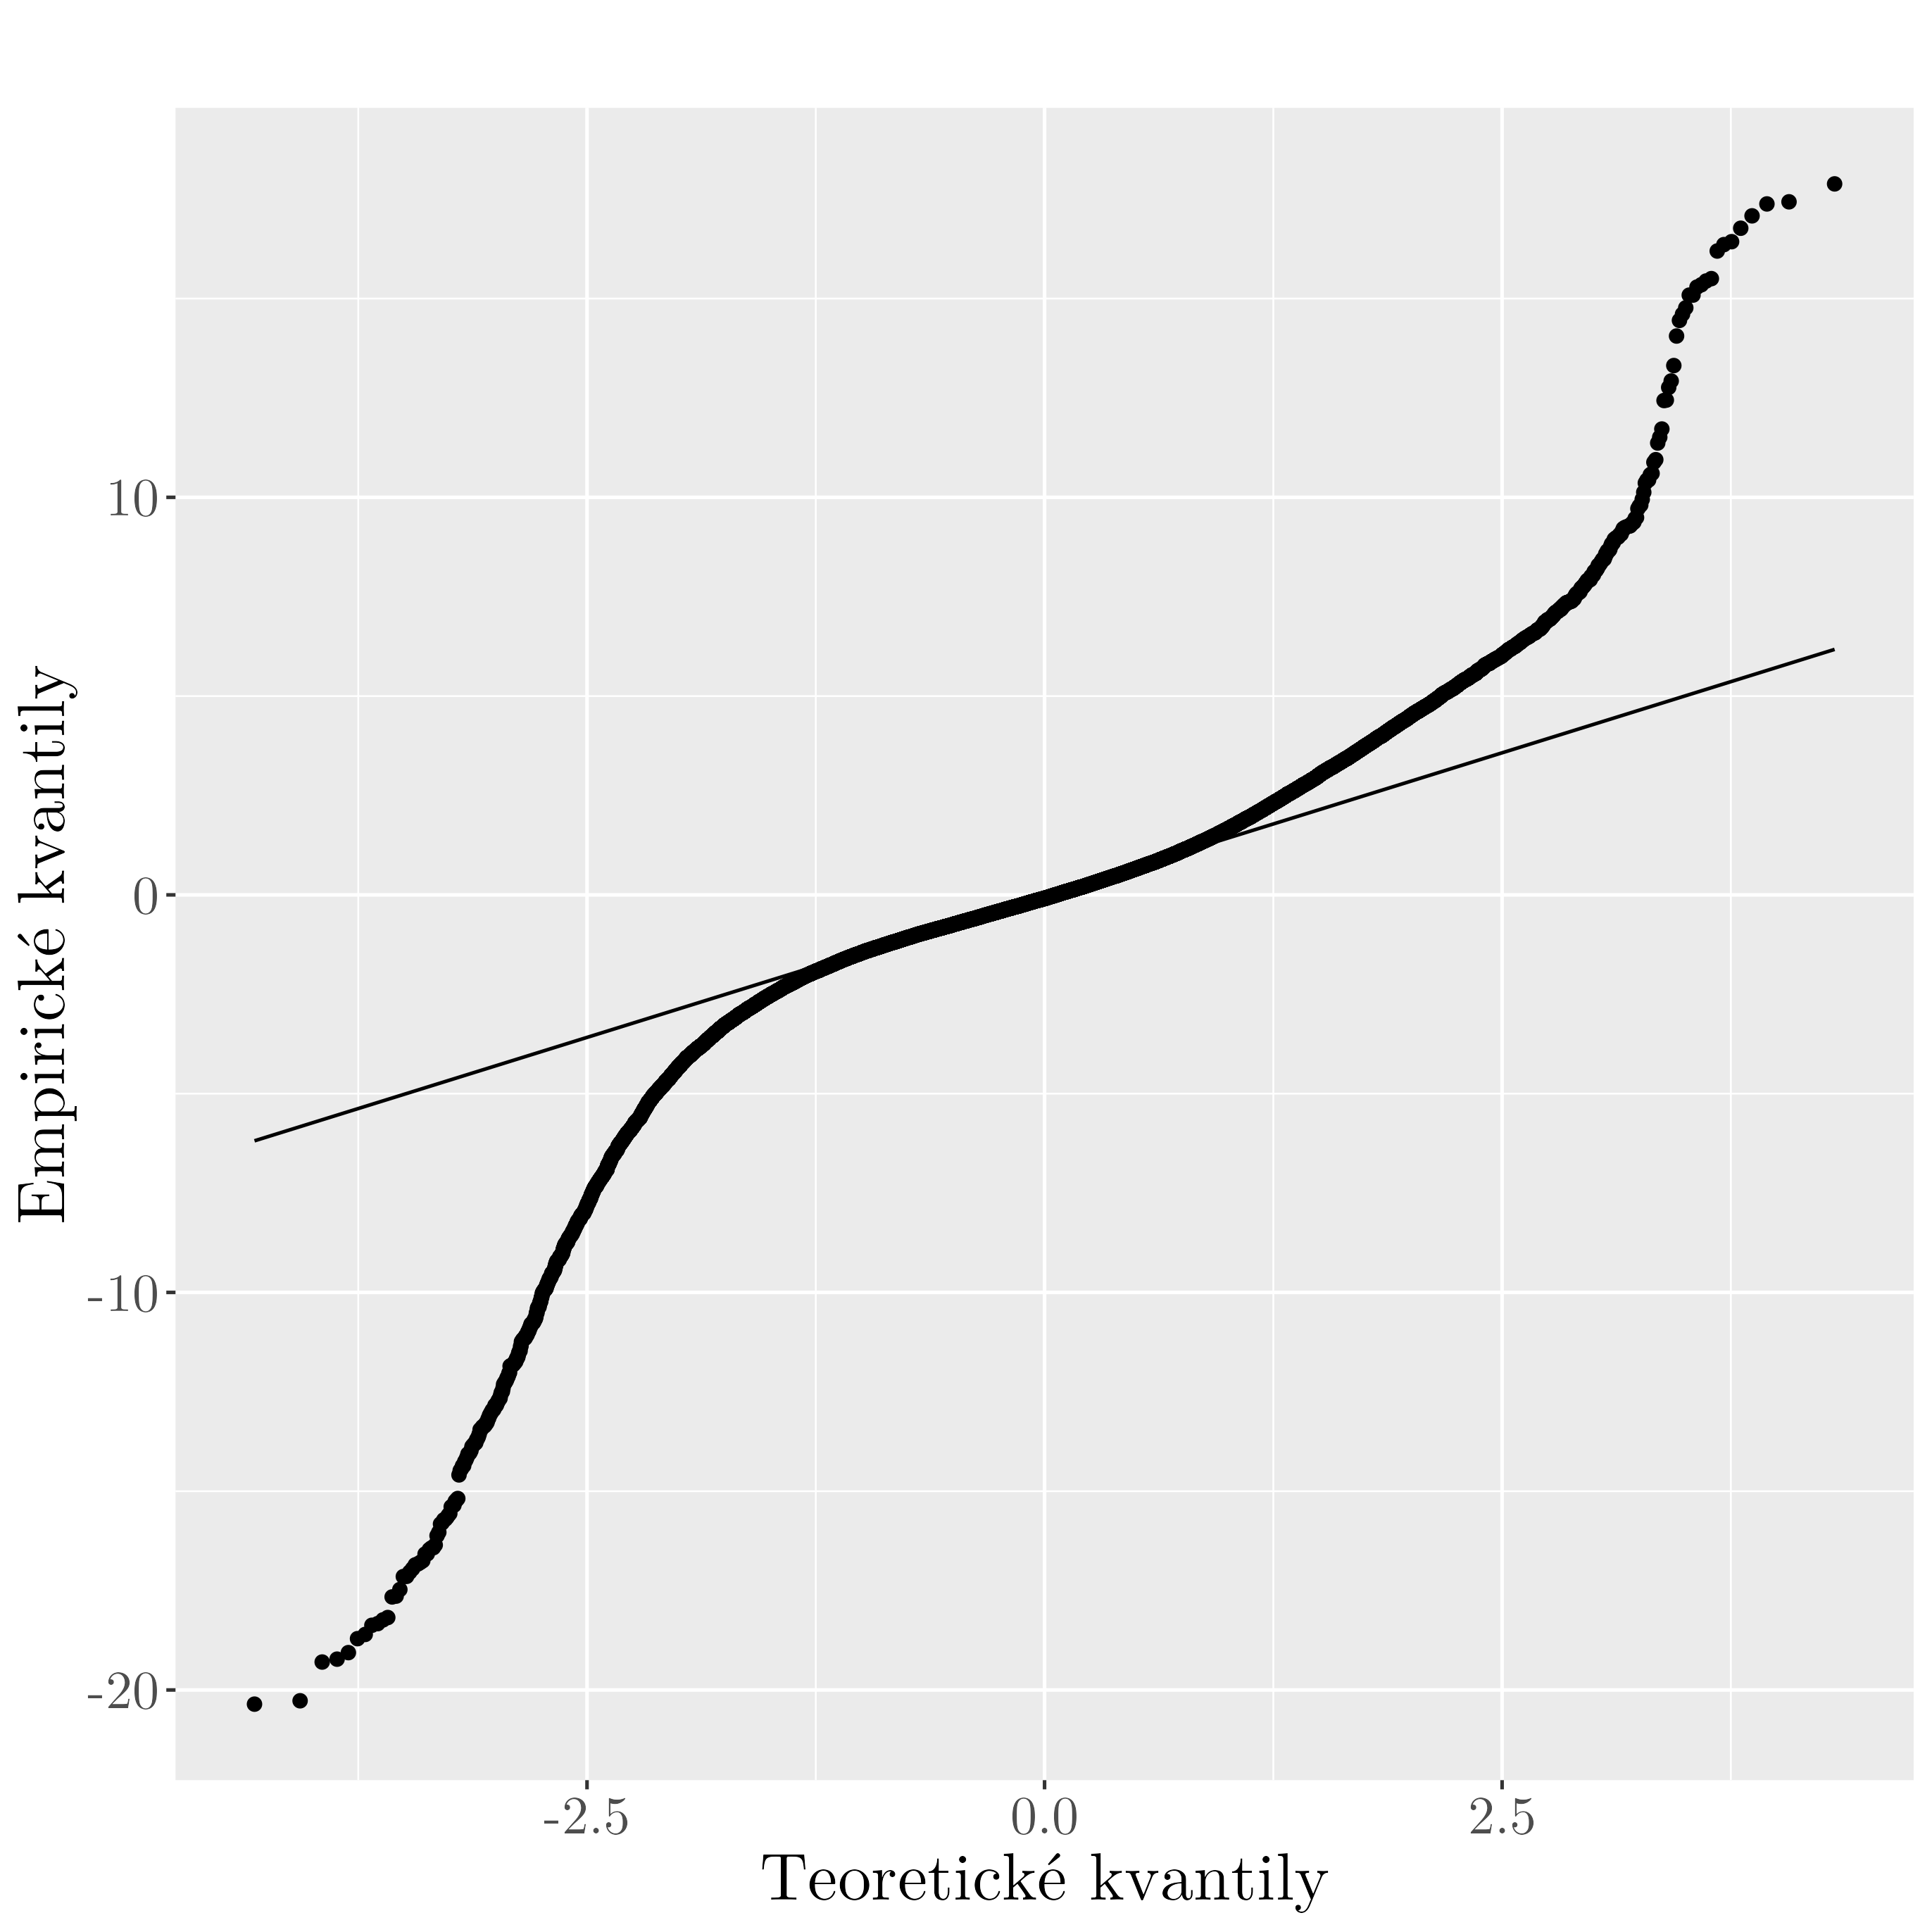
\includegraphics[width=\textwidth]{img/ch2/qq_modmax15cm_none.png}
		\caption{Bez transformace}
		\label{fig:qq_none}
	\end{subfigure}
	\hfill
	\begin{subfigure}{0.45\textwidth}
  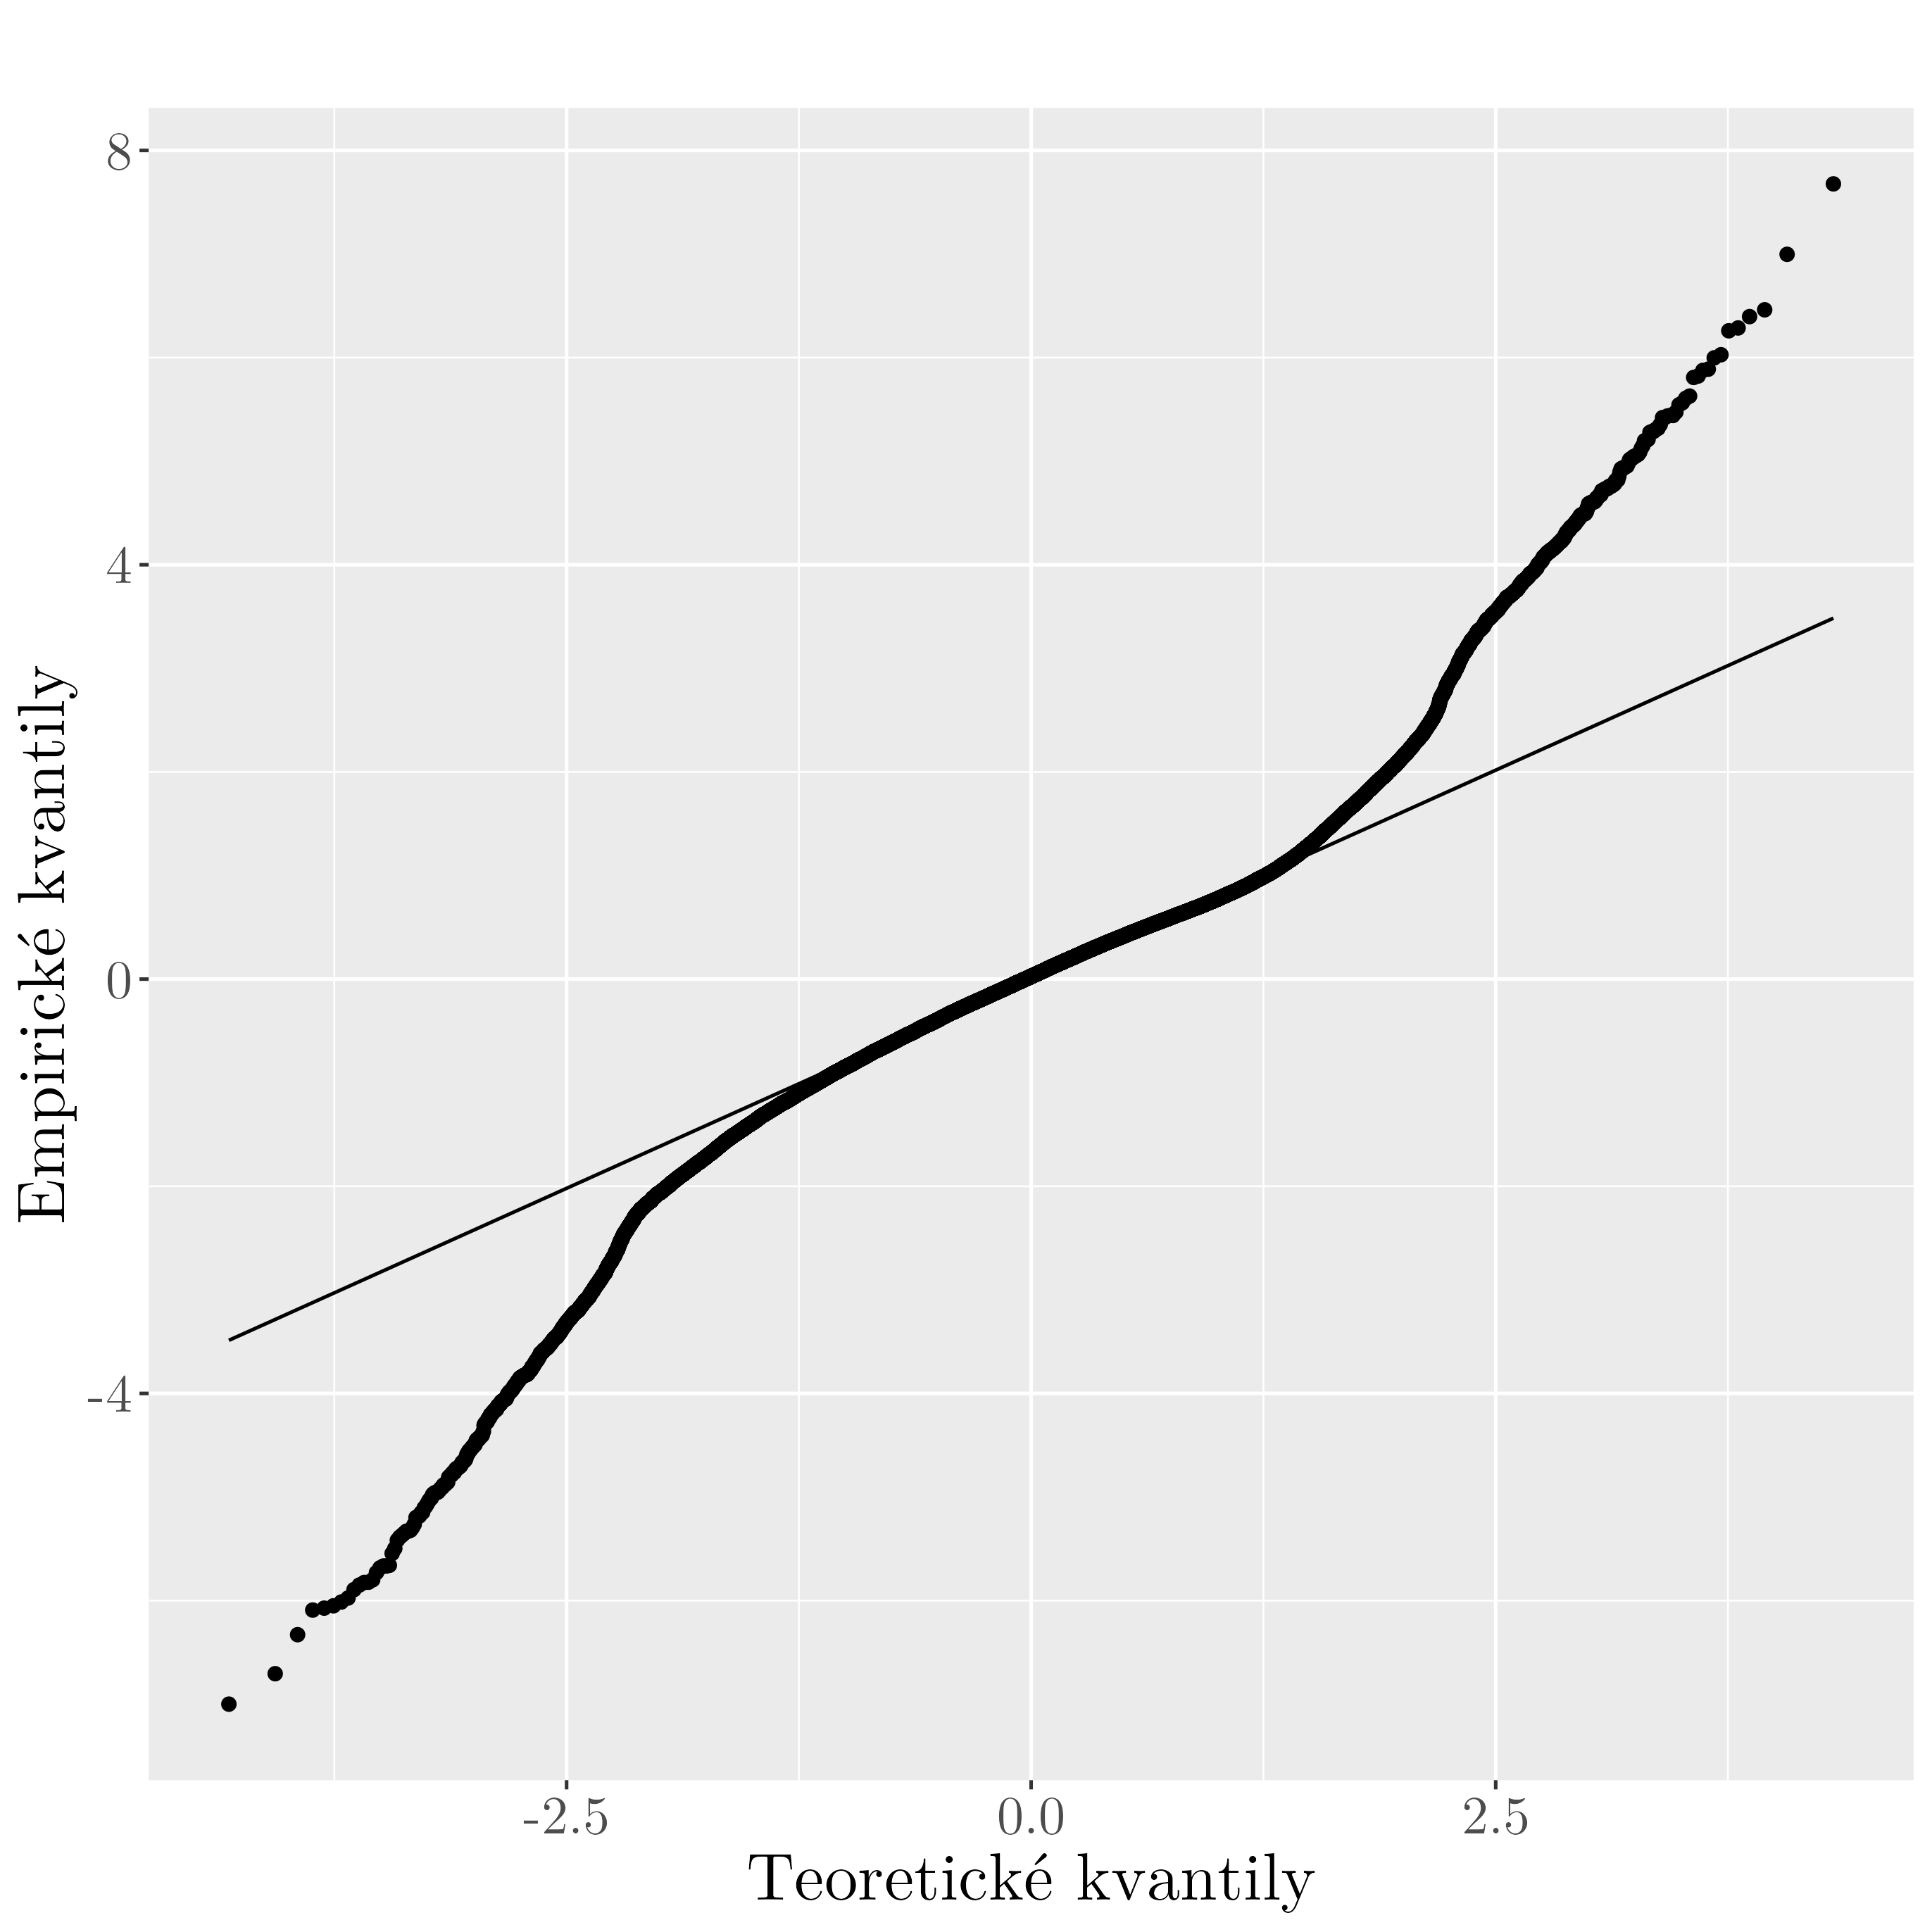
\includegraphics[width=\textwidth]{img/ch2/qq_modmax15cm_log.png}
		\caption{Přirozený logaritmus}
		\label{fig:qq_log}
	\end{subfigure}
	\hfill
	\begin{subfigure}{0.45\textwidth}
  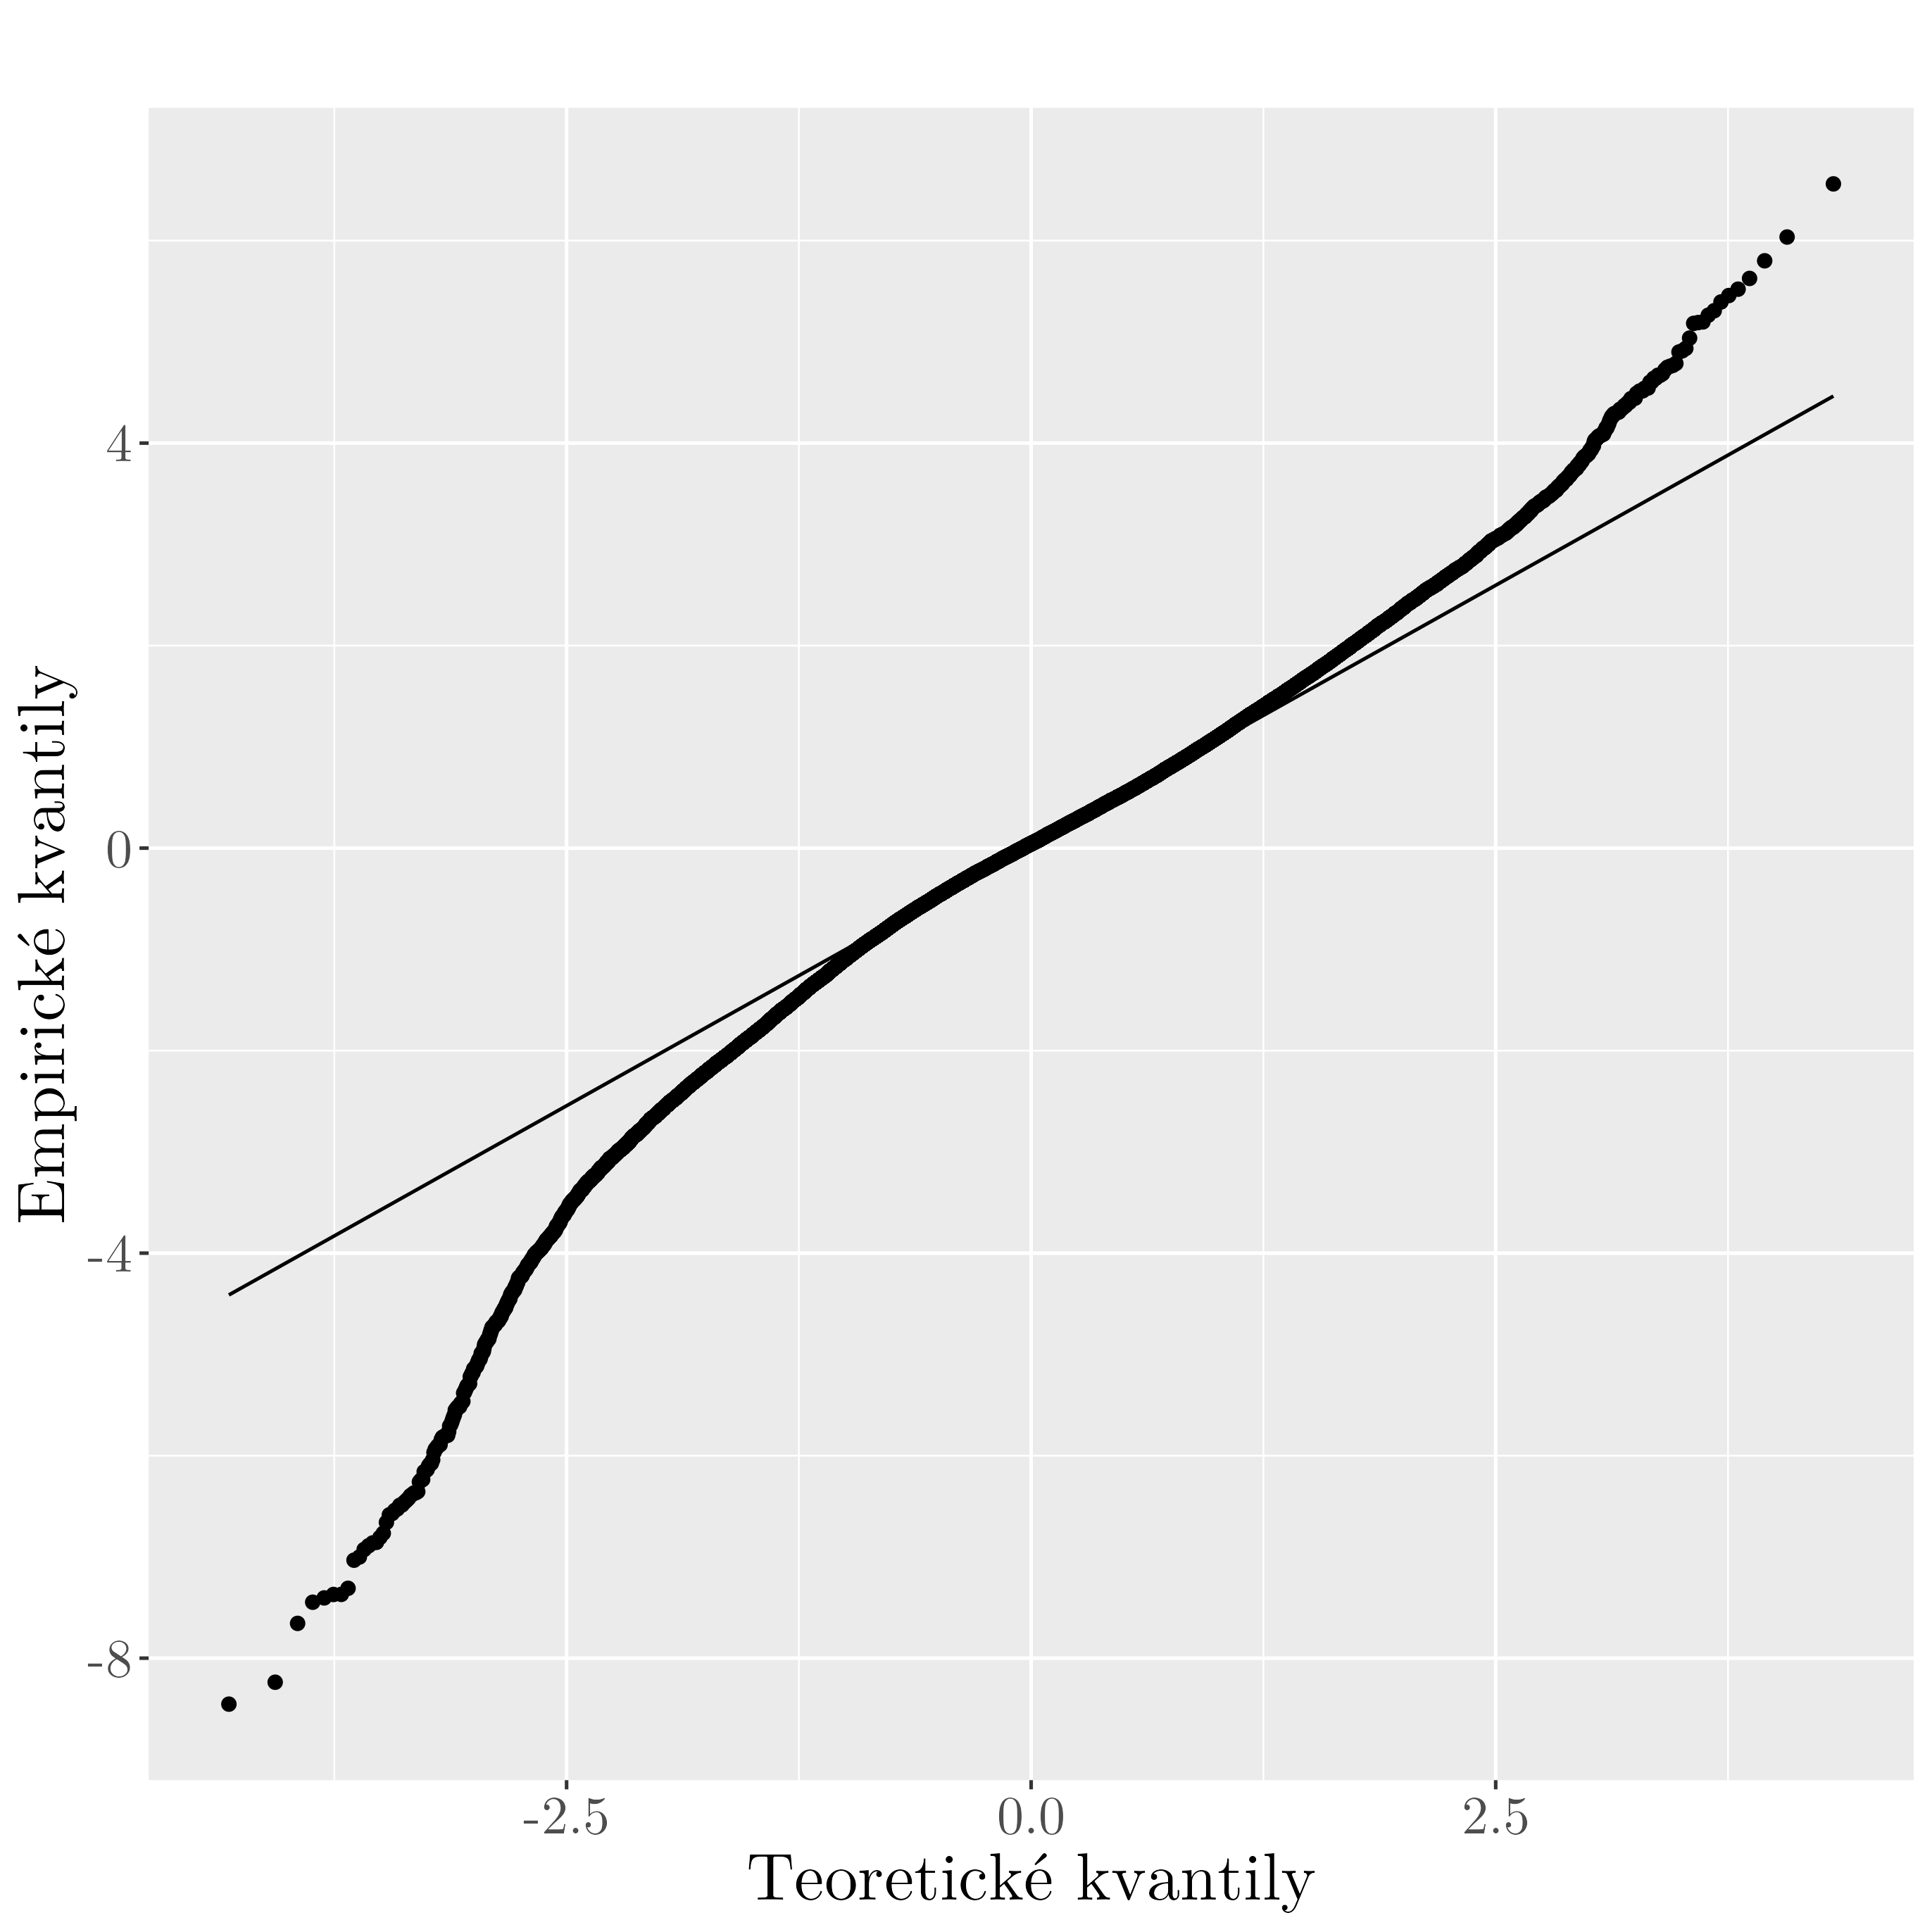
\includegraphics[width=\textwidth]{img/ch2/qq_modmax15cm_sqrt.png}
		\caption{Druhá odmocnina}
		\label{fig:qq_sqrt}
	\end{subfigure}
	\hfill
	\begin{subfigure}{0.45\textwidth}
  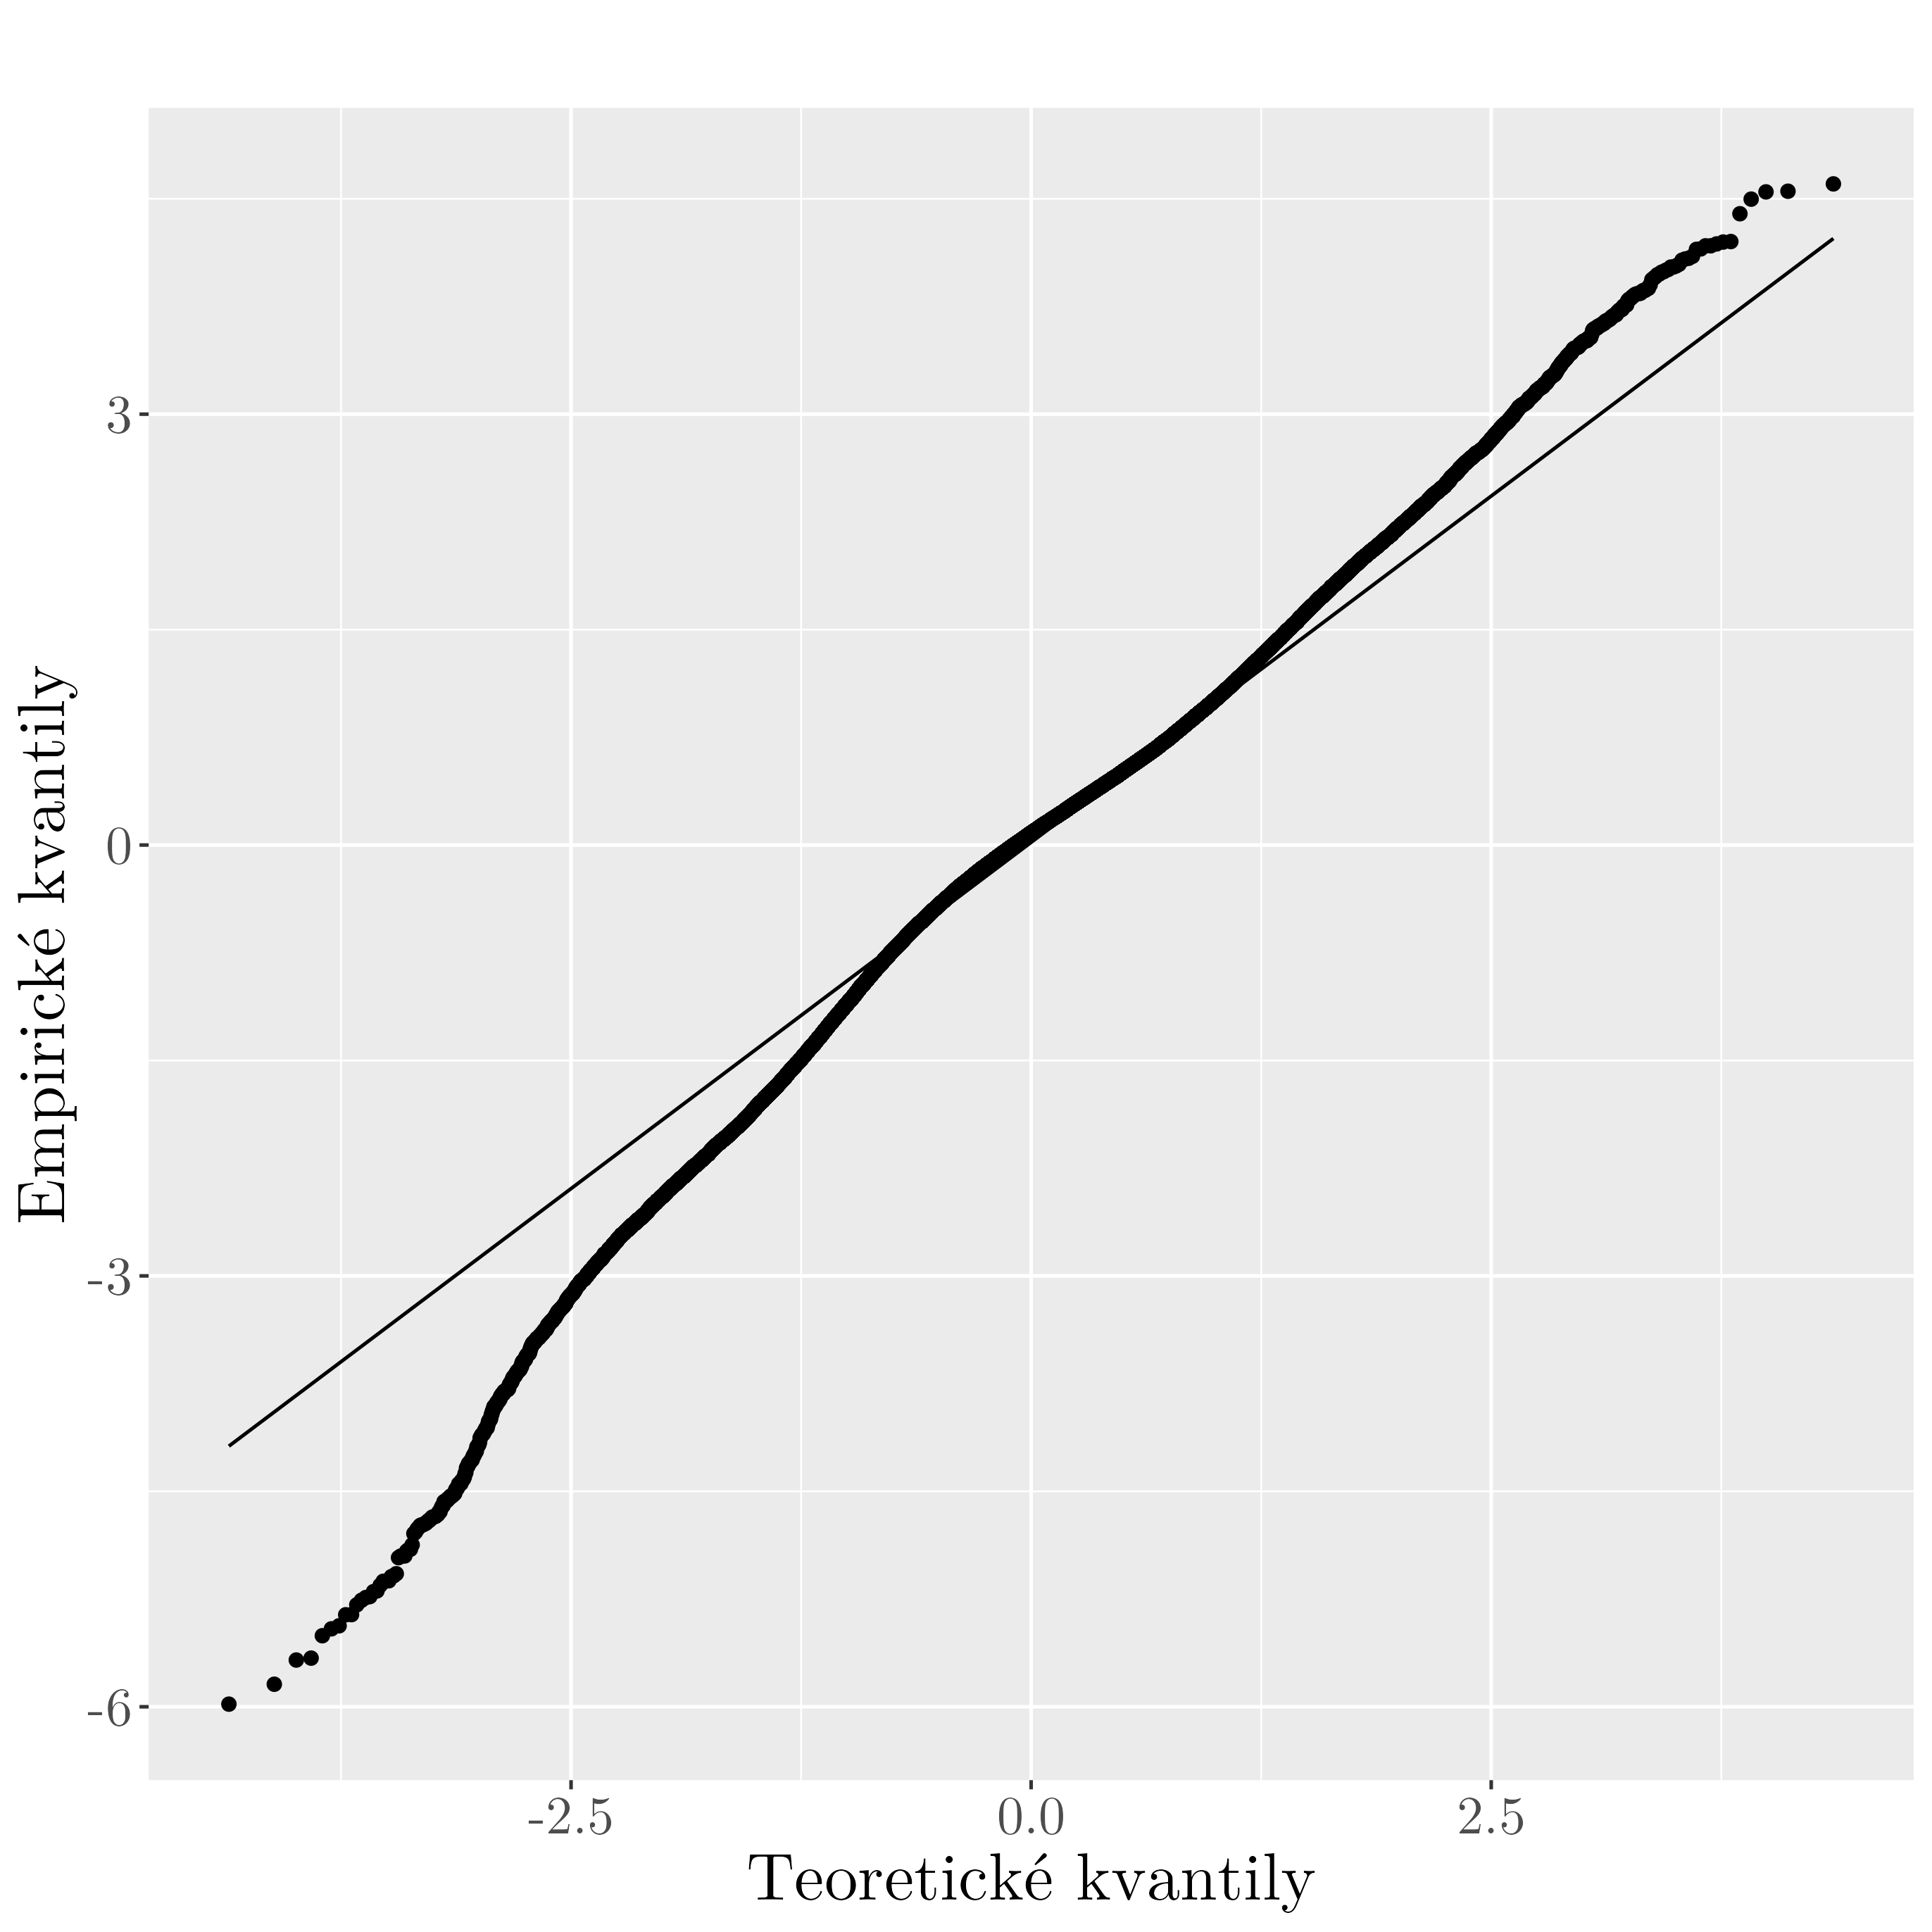
\includegraphics[width=\textwidth]{img/ch2/qq_modmax15cm_curt.png}
		\caption{Třetí odmocnina}
		\label{fig:qq_curt}
	\end{subfigure}
	\caption{Kvantil-kvantilový graf pro jednotlivé transformace vysvětlované proměnné.}
	\label{fig:qq}
\end{figure}

Vidíme, že nejlépe normálnímu rozdělení odpovídá transformace třetí odmocniny a proto s ní budeme nadále pracovat. Transformace ovšem není dokonalá, stále jsme se úplně nezbavili šikmosti (skewness). Na obrázku \ref{fig:resvsfit_curt} můžeme vidět srovnání residuálů modelu s fitovanými hodnotami. Na obrázku můžeme vidět, že v takto transformovaných datech není výrazná heteroskedasticita.

Homoskedasticitu budeme ověřovat graficky, pomocí srovnání fitovaných hodnot a residuálů modelu. Pokud nebyl porušen předpoklad homoskedasticity tak nesmíme pozorovat závislost mezi fitovanými hodnotami a residuály, jak bylo popsáno v kapitole \ref{chap:lme}. Na obrázku \ref{fig:resvsfit_curt} vidíme srovnání residuálů modelu s fitovanými hodnotami a není zde žádná výrazná heteroskedasticita.

\begin{figure}
	\centering
  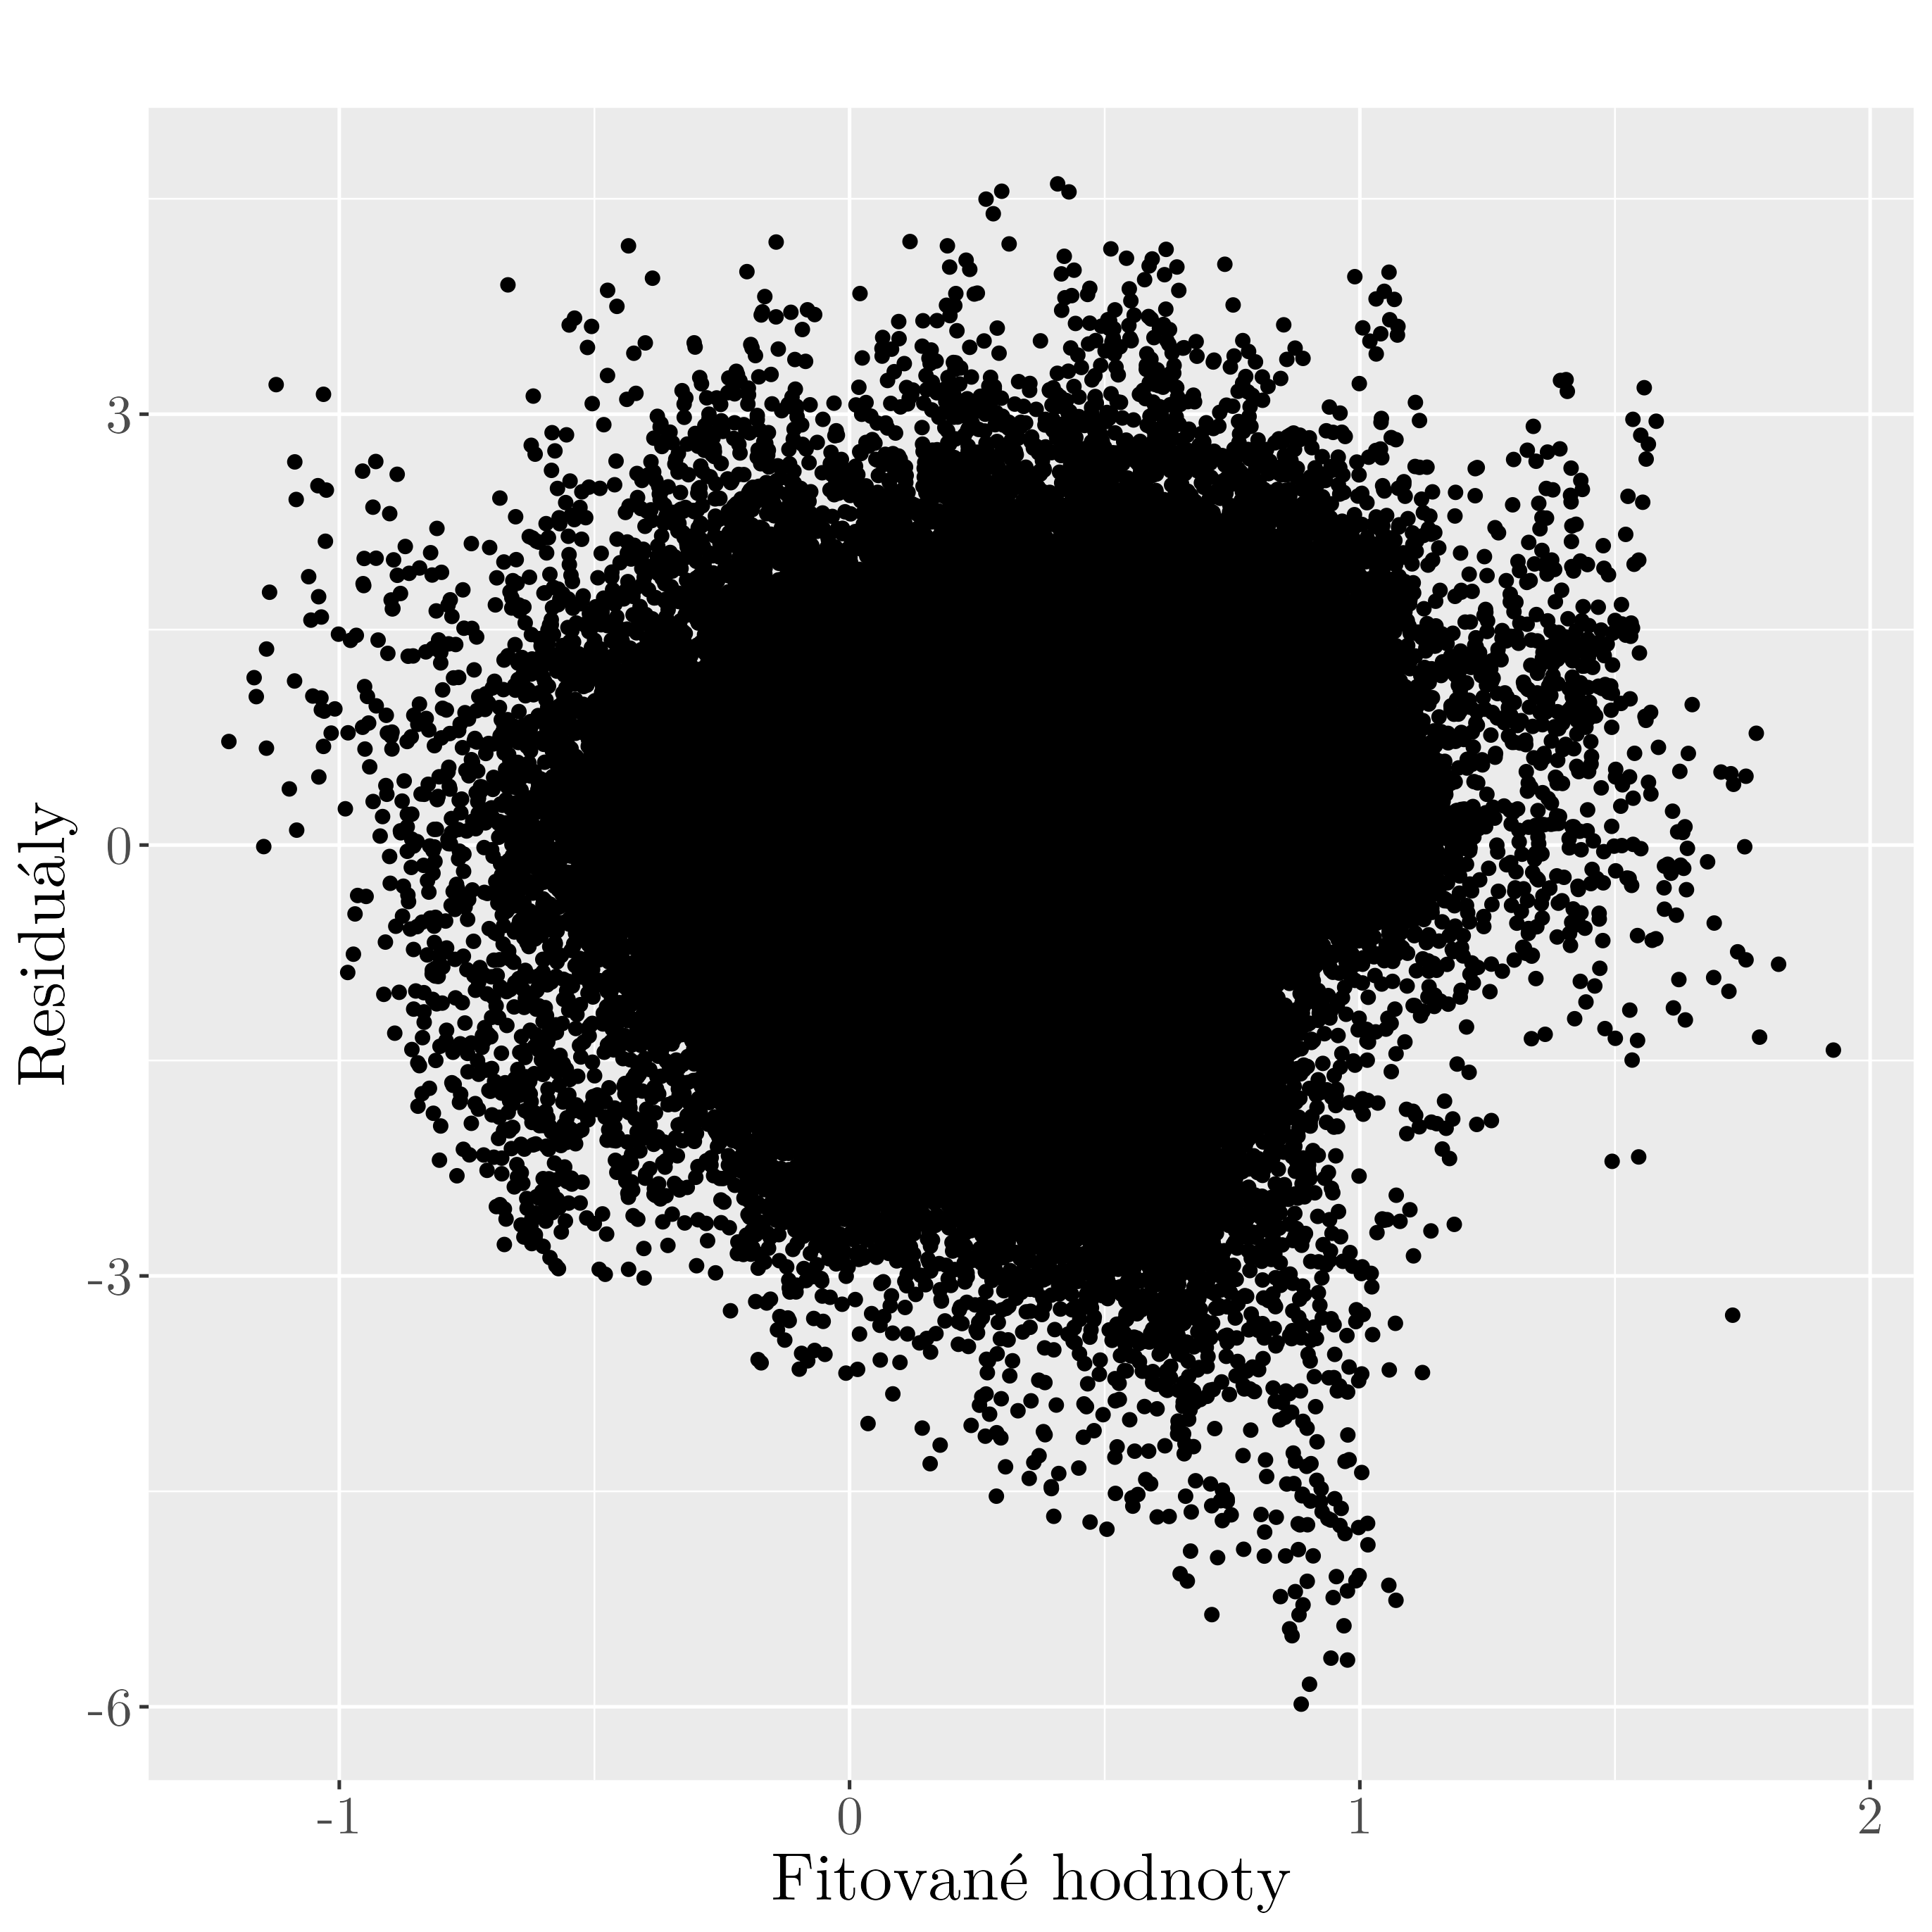
\includegraphics[width=0.55\textwidth]{img/ch2/modmax15cm_curt.png}
	\caption{Srovnání residuálů modelu s fitovanými hodnotami pro transformaci pomocí třetí odmocniny.}
	\label{fig:resvsfit_curt}
\end{figure}

Pro ilustraci důležitosti ARMA modelu na obrázku \ref{fig:acf_curtnoARMA} autokorelační funkci bez modelu ARMA a na \ref{fig:acf_curtARMA22} s modelem ARMA. Hodnota $\text{ACF}$ pro $\text{lag}=0$ je vyřazená pro větší přehlednost grafu, vždy nabývá hodnoty $1$.

Vidíme, že přidání ARMA s hodnotami se výrazně zlepší autokorelační funkce a korelační strukturu jsme téměř odfiltrovali. Testovali jsme i jiné hodnoty $p$ a $q$, ale pro tyto nám vyšla autokorelační funkce nejlepší. S rostoucím $p$ a $q$ také roste výpočetní náročnost, pro $p=3$ a $q=3$ se ACF téměř nezmění, ale výpočet trvá až 4-krát déle (na počítači, který byl používán ke spracování šlo o více než 2 hodiny výpočetního času).

\begin{figure}
	\centering
	\begin{subfigure}{0.45\textwidth}
  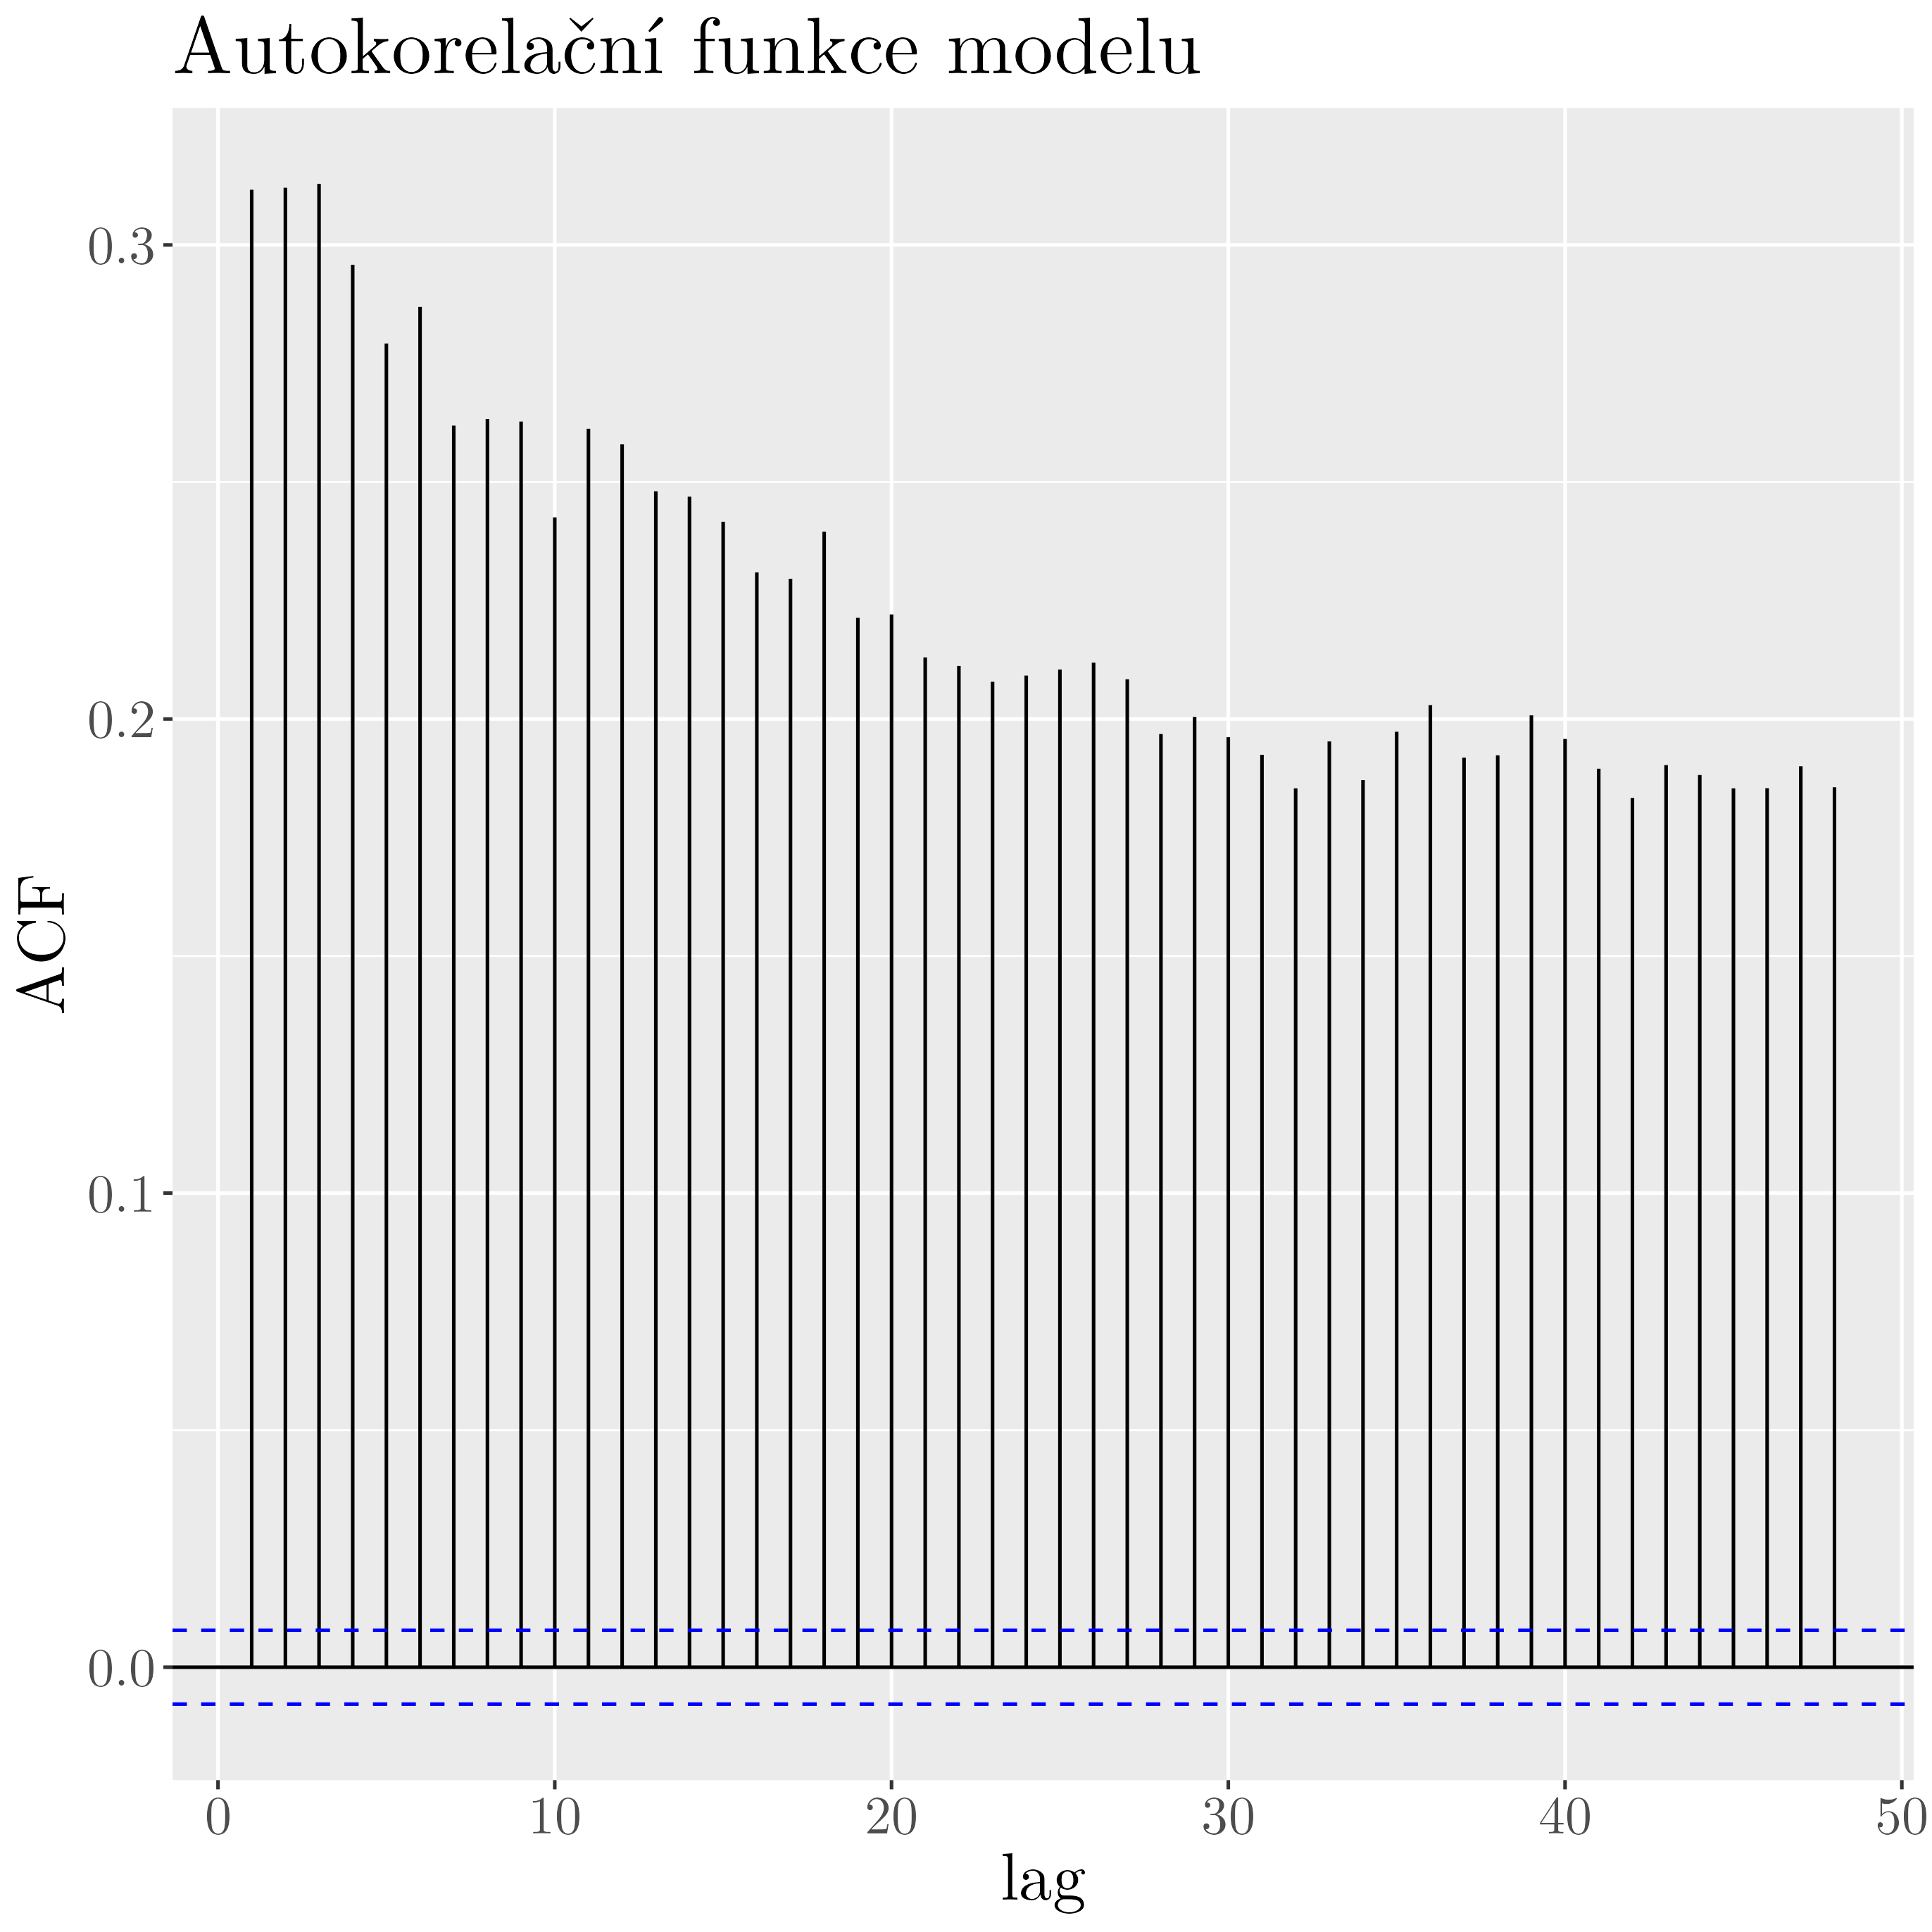
\includegraphics[width=\textwidth]{img/ch2/acf_curt.png}
		\caption{Autokorelační funkce pro model s transformací $\sqrt[3]{}$, ale bez modelování autokorelační struktury.}
		\label{fig:acf_curtnoARMA}
	\end{subfigure}
	\hfill
	\begin{subfigure}{0.45\textwidth}
  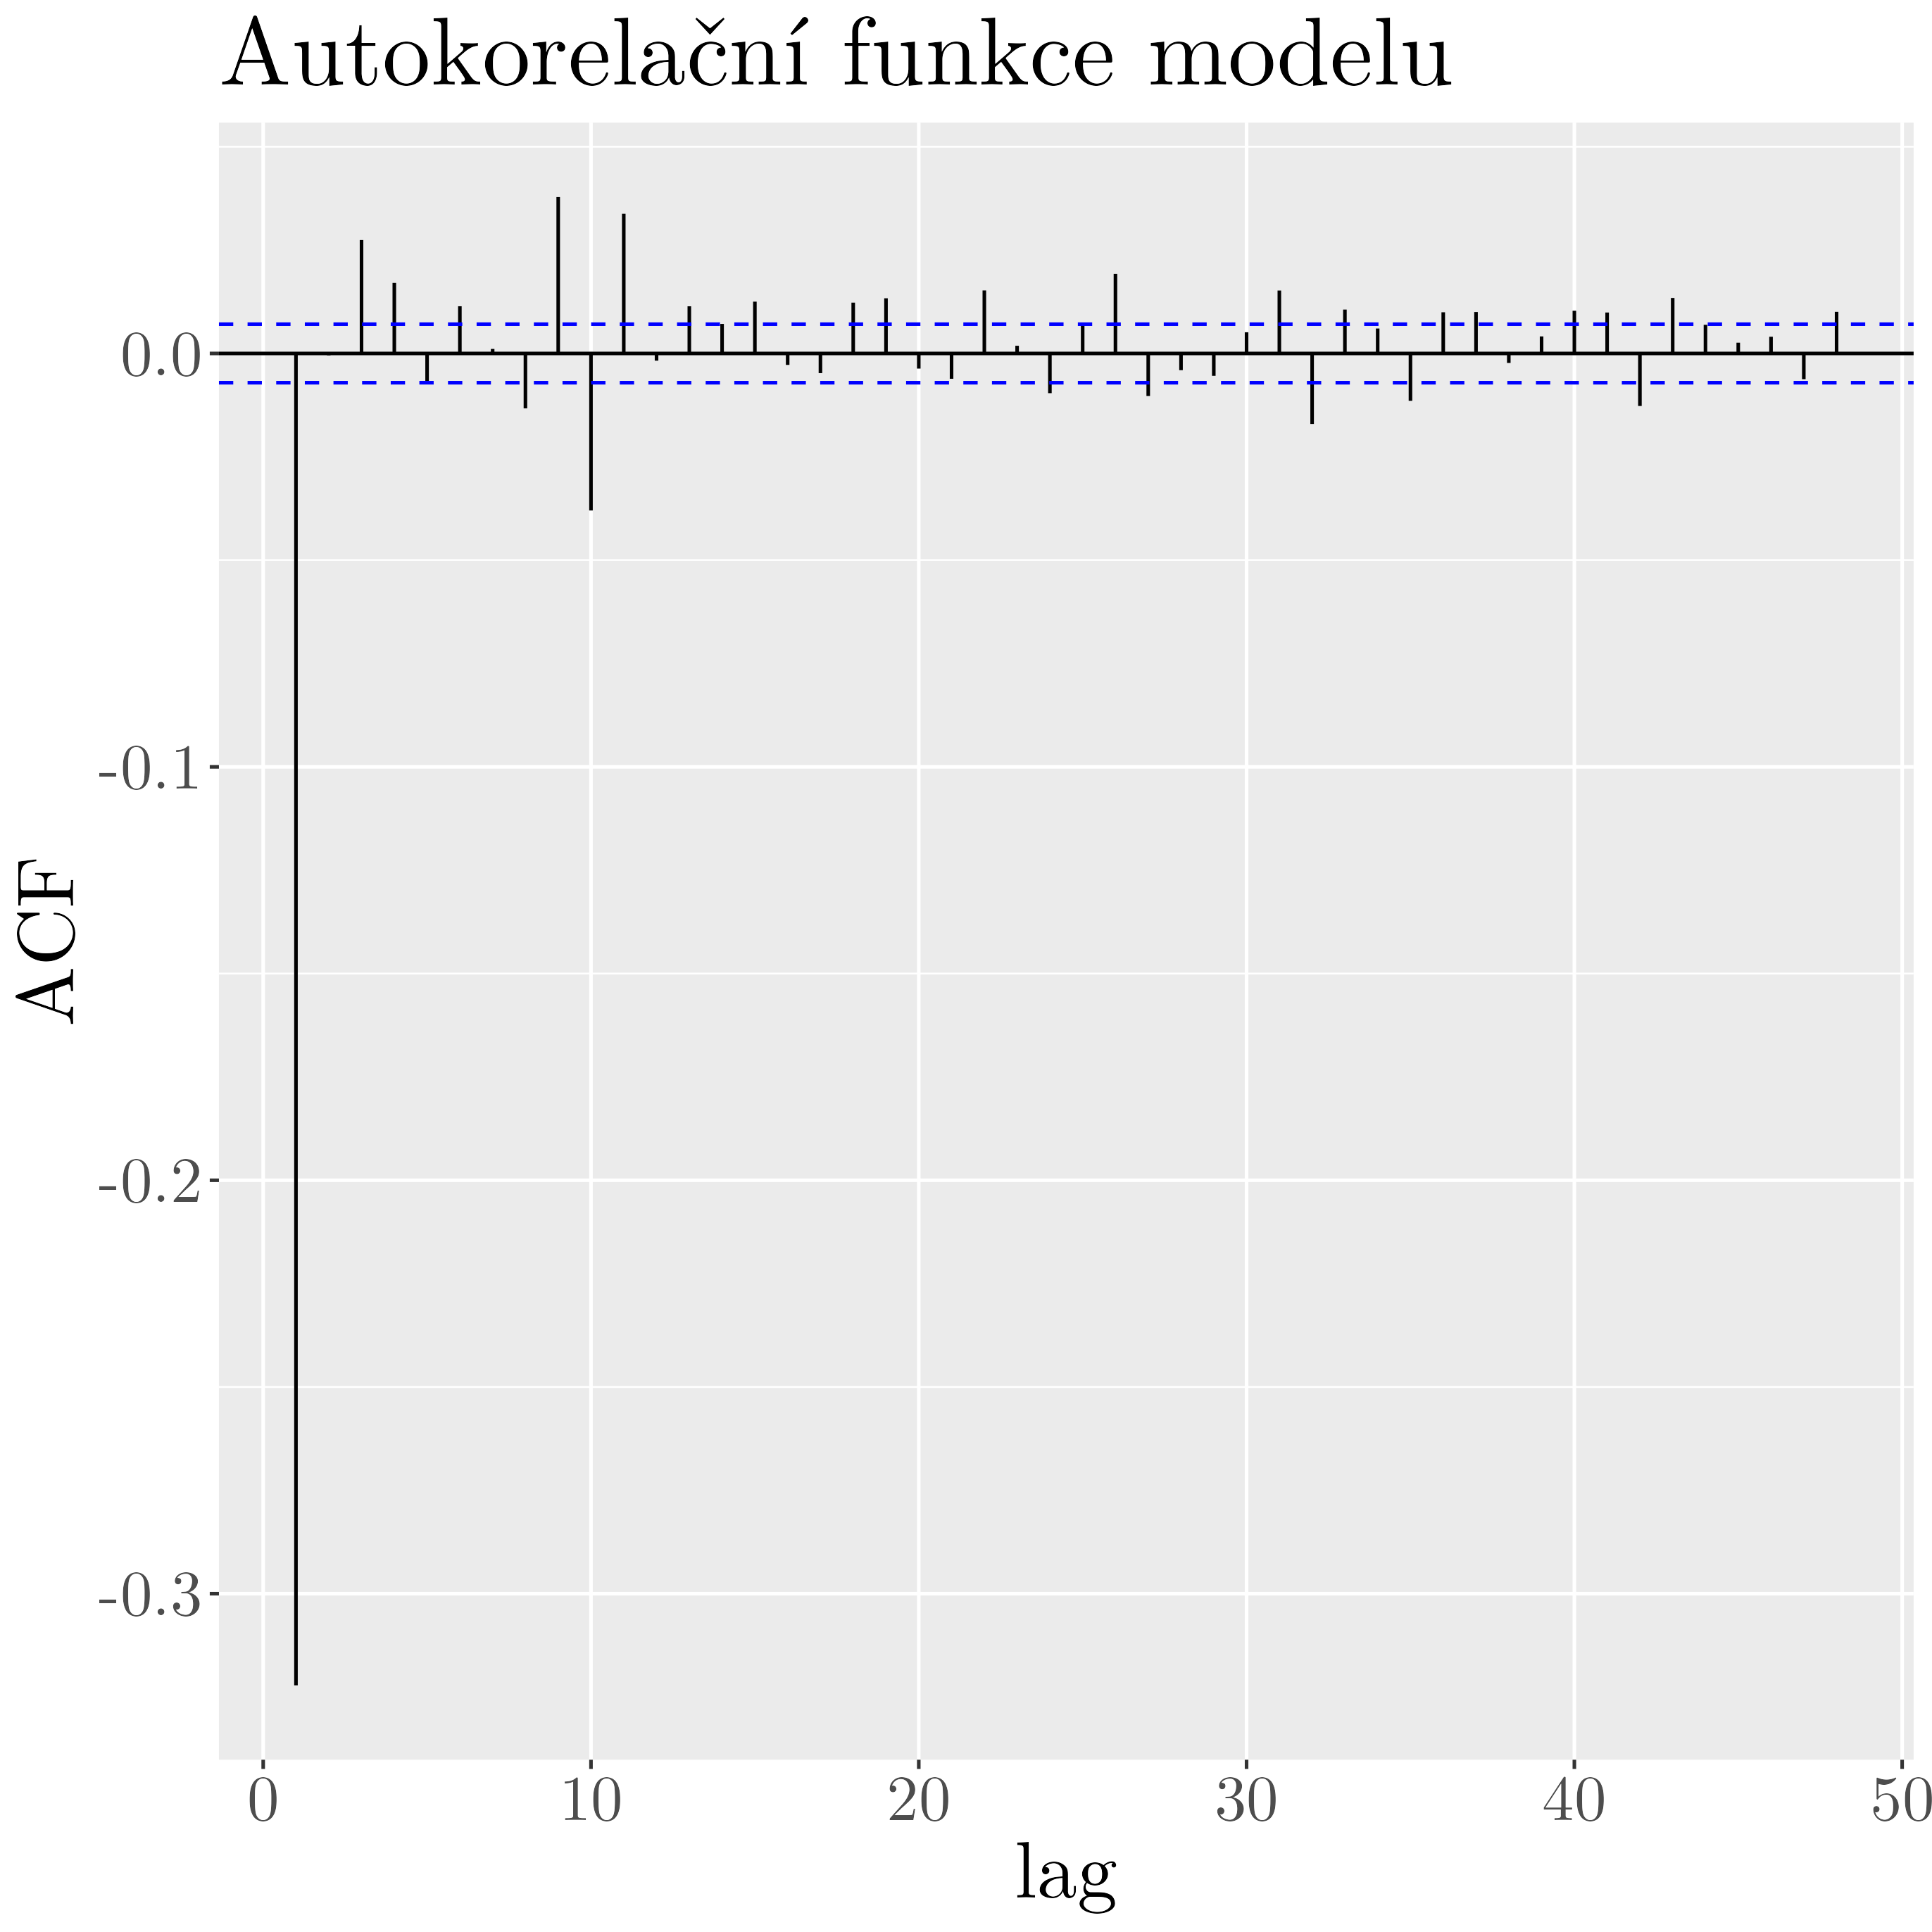
\includegraphics[width=\textwidth]{img/ch2/acf_curtARMA22.png}
		\caption{Autokorelační funkce pro model s transformací $\sqrt[3]{}$, s modelování autokorelační struktury, kde $p=2,\ q=2$.}
		\label{fig:acf_curtARMA22}
	\end{subfigure}
	\caption{Srovnání autokorelační funkce modelu s a bez ARMA}
	\label{fig:acf_curt}
\end{figure}
